\documentclass[11pt, openany]{book}
\usepackage[text={4.65in,7.45in}, centering, includefoot]{geometry}
\usepackage[table, x11names]{xcolor}
\usepackage{setspace}
\usepackage{multicol}
\usepackage{ragged2e}
\usepackage{multirow}
\usepackage{wrapfig}
\usepackage{fontspec,realscripts}
\usepackage{polyglossia}

\setdefaultlanguage{sanskrit}
\setotherlanguage{english}
\defaultfontfeatures[Scale=MatchUppercase]{Ligatures=TeX}

\newfontfamily\sanskritfont[Script=Devanagari]{Shobhika}
\newfontfamily\englishfont[Language=English, Script=Latin]{Linux Libertine O}
\newfontfamily\q[Script=Devanagari, Scale=0.95, Color=violet]{Shobhika-Regular}
\newfontfamily\ab[Script=Devanagari, Scale=1.05, Color=purple]{Shobhika-Bold}
\newfontfamily\eg[Script=Devanagari, Scale=1.05, Color=red]{Shobhika-Bold}
\newfontfamily\qt[Script=Devanagari, Scale=0.9, Color=violet]{Shobhika-Regular}
\newfontfamily\bqt[Script=Devanagari, Scale=1, Color=black]{Shobhika-Regular}
\newfontfamily\s[Script=Devanagari, Scale=0.9]{Shobhika-Regular}
\newcommand{\devanagarinumeral}[1]{%
 \devanagaridigits{\number\csname c@#1\endcsname}}
\usepackage{fancyhdr}
\pagestyle{fancy}
\renewcommand{\headrulewidth}{0pt}
\usepackage{enumerate}
%\pagestyle{plain}
\usepackage{afterpage}
\usepackage{amsmath}
\usepackage{amssymb}
\usepackage{graphicx}
\usepackage{longtable}
\usepackage{footnote}
\usepackage{dblfnote}
\usepackage{xspace}
%\newcommand\nd{\textsuperscript{nd}\xspace}
\usepackage{array}
\usepackage{emptypage}
\usepackage{hyperref}   % Package for hyperlinks
\hypersetup{
colorlinks,
citecolor=black,
filecolor=black,
linkcolor=blue,
urlcolor=black
}

\XeTeXgenerateactualtext=1 % for searchable pdf

\begin{document}
\s\onehalfspacing
 \fancyhead[CE] {बीजगणिते}
\fancyhead[CO]{वर्गप्रकृतिः}
\fancyhead[LE,RO]{\thepage}
\cfoot{}
\renewcommand{\thepage}{\devanagarinumeral{page}}
\setcounter{page}{114}

 एवं भावनाभ्यामिष्टक्षेपजपदसिद्धौ तेभ्य एव क्षेपान्तरजपदानयनमथ च यत्र 
कुत्रापि क्षेपपदसिद्धौ स चेदिष्टवर्गेण गुणितो भक्तो वोद्दिष्टक्षेपो
भवेत्तदा तेभ्य एवोद्दिष्टक्षेपजपदा-नयनमनुष्टुभाह\textendash

\phantomsection \label{72}
\begin{quote}
    \ab 
     इष्टवर्गहृतः क्षेपः क्षेपः स्यादिष्टभाजिते~। \\
 मूले ते स्तोऽथवा क्षेपः क्षुण्णः क्षुण्णे तदा पदे~॥~७२~॥
\end{quote}

यस्मिन्क्षेपे कनिष्ठज्येष्ठपदे सिद्धे स क्षेप इष्टस्य वर्गेण भक्तः
सन्यदि क्षेपो भवति तदा ते पदे इष्टभक्ते सती पदे स्तः~। यदि त्विष्टवर्गेण गुणितः 
सन्क्षेपो भवति तदा ते पदे इष्टगुणिते स्तः~। यस्येष्टस्य वर्गेण क्षेपो
गुणितस्तेन पदे गुणनीये इत्यर्थः~। अत्रोपपत्तिः~। वर्गराशिर्वर्गेण गुणितो भक्तो वा
वर्गत्वं न जहातीति सुप्रसिद्धम्~। प्रकृते कनिष्ठवर्गः कव १~। कनिष्ठवर्गः प्रकृतिगुणः
क्षेपयुतो ज्येष्ठवर्गो 
भवतीति जातो ज्येष्ठवर्गः कव ० प्र १ क्षे १~। अथोभयोरपीष्टवर्गेण
गुणितयोर्न्यासः~। 
\vspace{-1mm}

\begin{center}
    इव ० कव १ इव ० कव ० प्र १ इव ० क्षे १~। 
\end{center} 
\vspace{-1mm}

 अत्र कनिष्ठज्येष्ठवर्गयोरिष्टवर्गगुणनात्तत्पदयोरिष्टमेव गुणकः स्यात्
यतो यैवेष्टवर्गकनिष्ठवर्गहतिः स एवेष्टकनिष्ठाहतिवर्गः~। एवं ज्येष्ठवर्गेऽपि~। इष्टकनिष्ठाहतिवर्गस्य पदं त्विष्टकनिष्ठाहतिरेव स्यात्~। एवं ज्येष्ठवर्गस्यापि~।
अथात्र क्षेपविचारः~। 
प्रकृतिगुणस्य कनिष्ठवर्गस्य केवलस्य ज्येष्ठवर्गस्य च यदन्तरालं स हि
क्षेपः~। प्रकृते च तदन्तरालमिष्टवर्गहतः पूर्वक्षेपः~। एवमेवेष्टवर्गेण
कनिष्ठज्येष्ठवर्गयोर्हरणेऽपि~। तदेवमुपपन्नम् \hyperref[72]{\textbf{इष्टवर्गहृतः क्षेपः}} इत्यादि~॥~७२~॥~\\

\vspace{-2mm}
 अथ यत्र कुत्राप्युद्दिष्टक्षेपरूपक्षेपजपदाभ्यां भावनया पदानेकत्वं
भवतीति रूपक्षेपजपदसाधनं प्रकारान्तरेण सार्धानुष्टुभाह\textendash

\phantomsection \label{73}
\begin{quote}
    \ab 
      इष्टवर्गप्रकृत्योर्यद्विवरं तेन वा भजेत्~। \\
 द्विघ्नमिष्टं कनिष्ठं तत्पदं स्यादेकसंयुतौ~। \\
 ततो ज्येष्ठमिहानन्त्यं भावनातस्तथेष्टतः~॥~७३~॥

\end{quote}
\newpage
%%%%%%%%%%%%%%%%%%%%%%%%%%%%%%%%%%%%%%%%%%
इष्टवर्गप्रकृत्योर्यद्विवरं तेन द्विघ्नमिष्टं भजेत्~। तदेकसंयुतौ
रूपक्षेपे कनिष्ठं स्यात्ततः कनिष्ठाज्ज्येष्ठं स्यात् \hyperref[70]{\textbf{इष्टं ह्रस्वं तस्य वर्गः प्रकृत्या क्षुण्णः}} इत्यादिना~। 
इह कनिष्ठज्येष्ठयोर्भावनावशात्तथेष्टवशादानन्त्यमस्ति~। \\

\vspace{-4mm}
 अत्रोपपत्तिः~। इष्टं ह्रस्वमित्यत्रैवेष्टं कनिष्ठमित्युक्तम्~।
तच्चेद्द्विघ्नं तदा 
कनिष्ठवर्गश्चतुर्गुणः स्यात्~। असौ चतुर्गुणः
कनिष्ठवर्गप्रकृत्योश्चतुर्गुणो घातः~। 
अयं केन युतो मूलप्रदो भवतीति विचार्यते~। \hyperref[131]{\textbf{चतुर्गुणस्य घातस्य युतिवर्गस्य चान्तरम्~। राश्यन्तरकृतेस्तुल्यम्}} इति राश्यन्तरवर्गेण युतश्चतुर्गुणितो घातो
युतिवर्गो भवति~। तस्य चावश्यं मूललाभः~। अत्र तु कनिष्ठवर्गप्रकृत्योश्चतुर्गुणो घातोऽस्ति~। कनिष्ठं 
त्विष्टमेव~। अत इष्टवर्गप्रकृत्योश्चतुर्गणो घातोऽयम्~। असाविष्टवर्गेण
योजितश्चेदवश्यं मूलदः स्यात्~। तथा च द्विघ्नमिष्टं कनिष्ठम्~।
तस्मादिष्टवर्गप्रकृत्योरन्तरवर्गतुल्ये 
क्षेपे ज्येष्ठं पदमपि सिध्यति~। अपेक्षितं च रूपक्षेपे~। तत्र युक्तिः~।
\hyperref[72]{\textbf{इष्टवर्गहृतः क्षेपः क्षेपः स्यादिष्टभाजिते~। मूले ते स्तः}} इत्यनेन~।
अत्रेष्टवर्गप्रकृत्योर्विवरतुल्यमिष्टं कल्पितम्~। तद्वर्गेण क्षेपे भक्ते रूपमेव स्यात्~। कनिष्ठं
त्विष्टवर्गप्रकृत्योर्विवरेणैव भाज्यम्~। प्रकृते कनिष्ठं तु द्विघ्नमिष्टम्~। अत उपपन्नम्
\hyperref[73]{\textbf{इष्टवर्गप्रकृत्योर्यद्विववरं तेन वा भजेत्~। द्विघ्नमिष्टम्}} इति~॥~७३~॥~\\

\vspace{-2mm}
 अथ वर्गप्रकृतावुदाहरणद्वयमनुष्टुभाह\textendash
\begin{quote}
    \eg
    को वर्गोऽष्टहतः सैकः कृतिः स्याद्गणकोच्यताम्~। \\
 एकादशगुणः को वा वर्गः सैकः कृतिः सखे~॥~७४~॥~
\end{quote}

 स्पष्टोऽर्थः~। प्रथमे न्यासः प्र ८ क्षे १~। अत्रैकमिष्टं ह्रस्वं
प्रकल्प्य जाते मूले~। 
क १ ज्ये ३ क्षे १~। एतेषां भावनार्थं न्यासः\textendash \,$\begin{matrix}
\vspace{-1mm}
\mbox{{प्र ८ क १ ज्ये ३ क्षे १}}\\
\vspace{-1mm}
\mbox{{~~~ \,क १ ज्ये ३ क्षे १}}
\vspace{1mm}
\end{matrix}$ अत्र
सूत्रम् {\qt 'वज्राभ्यासौ ज्येष्ठलघ्वोः'} इत्यादि~। प्रथमकनिष्ठ\textendash \,१\textendash \,द्वितीयज्येष्ठमूल\textendash \,३\textendash \,अभ्यासः ३~। द्वितीयकनिष्ठप्रथमज्येष्ठयोः १~। ३ अभ्यासः ३~। अनयोरैक्यं कनिष्ठपदं स्यात्~। कनिष्ठयोः १~। १ आहतिः १ प्रकृति\textendash \,७\textendash \,गुणा ८ ज्येष्ठयोः ३~। ३ अभ्यासेनानेन ९ युता १९ ज्येष्ठपदं स्यात्~। क्षेपयोः १~। १
आहतिः क्षेपः १ स्यात्~। प्राङ्मूलक्षेपाणामेभिः सह भावनार्थं न्यासः\textendash \,$\begin{matrix}
\vspace{-1mm}
\mbox{{प्र ८ क १ ज्ये ३ क्षे १}}\\
\vspace{-1mm}
\mbox{{~~ क ६ ज्ये १७ क्षे १}}
\vspace{1mm}
\end{matrix}$~।

\newpage%%%%%%%%%%%%%%%%%%%%%%%%%%%%%%%%%%

\noindent अत्र वज्राभ्यासौ १७~। १८ अनयोरैक्यं ह्रस्वं ३५~। लघ्वोराहतिः ६ प्रकृत्या ८ क्षुण्णा  ४८ ज्येष्ठाभ्यासेन ५१ युक् ९९ ज्येष्ठमूलम्~। क्षेपयोरभ्यासः क्षेपः १~। क ३५ ज्ये ९९ क्षे १~। एवं भावनावशादानन्त्यम्~। अथ द्वितोयोदाहरणे न्यासः प्र ११ क्षे १~। रूपमिष्टं कनिष्ठं प्रकल्प्य तद्वर्गात्प्रकृतिगुणाद्रूपद्वयमपास्य मूलं ज्येष्ठं ३ भावनार्थं न्यासः~। $\begin{matrix}
\vspace{-1mm}
\mbox{{प्र ११ क १ ज्ये ३ क्षे २ं}}\\
\vspace{-1mm}
\mbox{{~~~~ क १ ज्ये ३ क्षे २ं}}
\vspace{1mm}
\end{matrix}$ ज्येष्ठलघ्वोर्वज्राभ्यासौ ३~। ३ 
अनयोरैक्यं ६ ह्रस्वम्~। लघ्वोः आहतिः १ प्रकृत्या क्षुण्णा ११
ज्येष्ठाभ्यासेन ९ युक् २० ज्येष्ठमूलम्~। क्षेपयोः २~। २ अभ्यासः ४ क्षेपः~। क ६ ज्ये २० क्षे ४ \hyperref[72]{\textbf{इष्टवर्गहृतः क्षेप}} इत्यादिना रूपद्वयमिष्टं प्रकल्प्य जाते
रूपक्षेपमूले क ३ ज्ये १० क्षे १~। समासभावनार्थं न्यासः $\begin{matrix}
\vspace{-1mm}
\mbox{{क ३ ज्ये १० क्षे १}}\\
\vspace{-1mm}
\mbox{{क ३ ज्ये १० क्षे १}}
\vspace{1mm}
\end{matrix}$ जाते मूले क ६० ज्ये १९९ क्षे १~। एवमत्र भावनावशादानन्त्यम्~। अथवा
रूपमिष्टं कनिष्ठं प्रकल्प्य जाते पञ्चक्षेपपदे क १ ज्ये ४ क्षे ५~।
अनयोस्तुल्यभावनया 
मूले क ८ ज्ये २७ क्षे २५ \hyperref[72]{\textbf{इष्टवर्गहृतः क्षेपः}} इति पञ्चकमिष्टं प्रकल्प्य जाते 
रूपक्षेपमूले क ज्ये क्षे १~। अनयोः पूर्वमूलाभ्यां सह भावनार्थं न्यासः~। $\begin{matrix}
\vspace{1mm}
\mbox{{प्र ११ क $\dfrac{\mbox{८}}{\mbox{५}}$ ज्ये $\dfrac{\mbox{२७}}{\mbox{५}}$ क्षे १}}\\
\vspace{-1mm}
\mbox{{~~~~ क ३ ~ज्ये १० क्षे १}}
\vspace{1mm}
\end{matrix}$ भावनया लब्धे मूले क $\dfrac{\mbox{१६१}}{\mbox{५}}$ ज्ये $\dfrac{\mbox{५३४}}{\mbox{५}}$ क्षे १~। अथवा \hyperref[71]{\textbf{ह्रस्वं वज्राभ्यासयोरन्तरम्}} इत्यादिना कृतयान्तरभावनया जाते मूले क $\dfrac{\mbox{१}}{\mbox{५}}$  ज्ये $\dfrac{\mbox{६}}{\mbox{५}}$ क्षे १~। एवमनेकधा~। 
\hyperref[73]{\textbf{इष्टवर्गप्रकृत्योर्यद्विवरं तेन भजेत्}} इत्यादिना पक्षान्तरेण पदे रूपक्षेपे प्रतिपाद्येते~। 
प्रथमोदाहरणे रूपत्रयमिष्टं प्रकल्प्य यथोक्तकरणे कनिष्ठं ६ अस्य वर्गः
३६ प्रकृति\textendash \,८\textendash \,गुणः २८८ सैको २८६ अस्य मूलं १७ ज्येष्ठपदम्~। एवं द्वितीयोदाहरणेऽपि 
रूपत्रयमिष्टं प्रकल्प्य जाते कनिष्ठज्येष्ठे क ३ ज्ये १० क्षे १~।
एवम् इष्टवशात् समः सान्तरभावनाभ्यां च पदानाम् आनन्त्यम्~॥~७४~॥~\\

\vspace{-2mm}
 अथ कनिष्ठज्येष्ठयोरभिन्नतार्थं चक्रवालाख्यां वर्गप्रकृतिमनुष्टुभ
उत्तरार्धेनानुष्टुप्त्रितयेनानुष्टुप्पूर्वार्धेन चाह\textendash\
\newpage
%%%%%%%%%%%%%%%%%%%%%%%%%%%%%%%%%%%%%%%%%%%%%

\phantomsection \label{75}
\begin{quote}
    \ab 
      ह्रस्वज्येष्ठपदक्षेपान्भाज्यप्रक्षेपभाजकान्~। \\
 कृत्वा कल्प्यो गुणस्तत्र तथा प्रकृतितश्च्युते~। \\
 गुणवर्गे प्रकृत्योनेऽथवाल्पं शेषकं यथा~। \\
 तत्तु क्षेपहृतं क्षेपो व्यस्तः प्रकृतितश्च्युते~। \\
 गुणलब्धिः पदं ह्रस्वं ततो ज्येष्ठमतोऽसकृत्~। \\
 त्यक्त्वा पूर्वपदक्षेपांश्चक्रवालमिदं जगुः~। \\
 चतुर्द्व्येकयुतावेवमभिन्ने भवतः पदे~। \\
 चतुर्द्विक्षेपमूलाभ्यां रूपक्षेपार्थभावना~॥~७५~॥~
\end{quote}

 प्रथमतः \hyperref[70]{\textbf{इष्टं ह्रस्वं तस्य वर्गः}} इत्यादिना
ह्रस्वज्येष्ठक्षेपान्कृत्वा पश्चात्तान् ह्रस्वज्येष्ठक्षेपान्क्रमेण भाज्यक्षेपभाजकान्कृत्वा कुट्टकेन तथा गुणः साध्यो यथा  गुणस्य वर्गे प्रकृतितश्च्युते प्रकृत्योने वा शेषकमल्पं स्यात्~। तत्तु
शेषं पूर्वक्षेपहृतं सत्क्षेपः स्यात्~। गुणवर्गे प्रकृतितश्च्युते सत्ययं
क्षेपो व्यस्तः स्यात्~। 
धनं चेदृणमृणं चेद्धनं भवेदित्यर्थः~। यस्य गुणस्य वर्गेण प्रकृत्या
सहान्तरं कृतं तस्य गुणस्य या लब्धिस्तत्कनिष्ठं पदं स्यात्~। ततः
कनिष्ठाज्ज्येष्ठं 
पूर्ववत्स्यात्~। अथ प्रथमकनिष्ठज्येष्ठक्षेपांस्त्यक्त्वाधुना
साधितेभ्यः पुनः कुट्टकेन 
गुणाप्ती आनीयोक्तात्कनिष्ठज्येष्ठपदक्षेपाः साध्याः~। एवमसकृत्~। आचार्या
एतद्गणितं चक्रवालमिति जगुः~। एवं चक्रवालेन चतुर्द्व्येकयुतौ चतुःक्षेपे
द्विक्षेपे एकक्षेपे च भिन्ने पदे भवतः~। इदमुपलक्षणम्~। यत्र कुत्रापि क्षेपेऽभिन्ने
पदे भवतः~। युतावित्युपलक्षणम्~। तेन शुद्धावपीति ज्ञेयम्~। अथ
रूपक्षेपपदानयने प्रकारान्तरमप्यस्तीत्याह\textendash \,\hyperref[75]{\textbf{चतुर्द्विक्षेपमूलाभ्याम्}} इति~।
चतुःक्षेपमूलाभ्यां द्विक्षेपमूलाभ्यां 
च रूपक्षेपार्थं भावना रूपक्षेपार्थभावना~। कार्येति शेषः~।
चतुःक्षेपे \hyperref[72]{\textbf{इष्टवर्गहृतः क्षेपः}} इत्यादिना द्विक्षेपे तु तुल्यभावनया चतुःक्षेपपदे प्रसाध्य
पश्चात् \hyperref[72]{\textbf{इष्टवर्गहृतः क्षेपः}} इत्यादिना रूपक्षेपजे पदे वा भवत इत्यर्थः~। एवं
नवत्र्यादिक्षेपमूलाभ्यामपि 
रूपक्षेपार्थभावना द्रष्टव्या~। अस्मिन् रूप-क्षेपपदानयने
तयोर्नाभिन्नत्वनियमः~। 
चतुर्द्विक्षेपमूलाभ्यां तु रूपक्षेपार्थभावनायां कनिष्ठयोर्द्वयं हर इति
प्रायो रुपक्षेपपदयोरभिन्नत्वं सिध्यतीति चतुर्द्विक्षेपमूलाभ्यामित्युक्तम्~।
यदा तु भावनया
 \newpage
 %%%%%%%%%%%%%%%%%%%%%%%%%%%%%%%%%%

\noindent भिन्नत्वं न सिध्येत्तदा पुनश्चक्रवालेनैव पदे साध्ये इति परमपि
सुधीभिरूह्यम्~।
अत्रोप-पत्तिः~। \hyperref[72]{\textbf{इष्टवर्गहृतः क्षेपः}} इत्यादियुक्त्या कनिष्ठमिष्टगुणितं चेदिष्टवर्गेण क्षेपोऽपि गुणनीयः~। तथा सति जातौ कनिष्ठक्षेपौ इ ० क १~। इव ० क्षे १~।
अत्र क्षेपतुल्यमिष्टं प्रकल्प्य \hyperref[72]{\textbf{इष्टवर्गहृतः क्षेपः}} इत्यादिना जातौ कनिष्ठक्षेपौ $\begin{matrix}
\vspace{-1mm}
\mbox{{इ ० क १~।}}\\
\vspace{-1mm}
\mbox{{~~~ क्षे १~।}}
\vspace{1mm}
\end{matrix}$ $\begin{matrix}
\vspace{-1mm}
\mbox{{इव ० क्षे १~।}}\\
\vspace{-1mm}
\mbox{{~~~ क्षेव १~।}}
\vspace{1mm}
\end{matrix}$ एवम् अत्र प्रथमकनिष्ठमिष्टगुणं क्षेपभक्तं कनिष्ठं
स्यात्~। कनिष्ठवज्ज्येष्ठमपि प्रथमक्षेपस्त्विष्टवर्गगुणितः क्षेपवर्गभक्तः
सन् अत्र क्षेपः स्यात्~। अत्र क्षेपे हारभाज्ययोः पूर्वक्षेपेणापवर्ते जातः क्षेपः $\begin{matrix}
\vspace{-1mm}
\mbox{{इव १}}\\
\vspace{-1mm}
\mbox{{क्षे १}}
\vspace{1mm}
\end{matrix}$ प्रथमक्षेपभक्त इष्टवर्गः~। 
तस्मात् इष्टगुणं कनिष्ठं क्षेपभक्तं सद्यदि कनिष्ठं कल्प्यते तर्हि
इष्टवर्गः क्षेपभक्तः सन् क्षेपो भवति~। अत्रेष्टं तादृशं कल्पनीयं येन गुणितं कनिष्ठं
क्षेपभक्तं शुध्येत्~। अन्यथा कनिष्ठमभिन्नं कथं स्यात्~। तदर्थं कनिष्ठं केन गुणितं
क्षेपभक्तं निःशेषं स्यादिति कनिष्ठं भाज्यं प्रकल्प्य क्षेपं हारं च
प्रकल्प्य क्षेपाभावे गुणाप्ती साध्ये~। अत्र या लब्धिस्तत् कनिष्ठपदम्~। योऽत्र
गुणस्तदेवेष्टमिति गुणकवर्गः पूर्वक्षेपभक्तः क्षेपः स्यात्~। ज्येष्ठमपि
गुणगुणितं क्षेपभक्तं ज्येष्ठं स्यात्~। अत्र क्षेपो महान् भवतीत्याचार्येणान्यथा यतितम्~।
कनिष्ठं भाज्यम्~। ज्येष्ठपदं क्षेपम्~। क्षेपं हरं च प्रकल्प्य गुणाप्ती साधिते~।
पूर्वं तु गुणगुणितं कनिष्ठं क्षेपभक्तं सत्कनिष्ठं भवतीति स्थितम्~।
इदानीं तु गुणगुणितं कनिष्ठं ज्येष्ठयुतं क्षेपभक्तं सत्कनिष्ठं स्यात्~।
तस्माज्ज्येष्ठं क्षेपभक्तं सत्कनिष्ठेऽधिकं जातम्~। एवं सति प्रकृतिगुणे कनिष्ठवर्गे
किमधिकं भवतीति विचार्यते~। तत्र पूर्वकनिष्ठं $\begin{matrix}
\vspace{-1mm}
\mbox{{इ ० क १}}\\
\vspace{-1mm}
\mbox{{~~ क्षे १}}
\vspace{1mm}
\end{matrix}$~। अस्य वर्गः $\begin{matrix}
\vspace{-1mm}
\mbox{{इव ० कव १}}\\
\vspace{-1mm}
\mbox{{~~~~~ क्षेप १}}
\end{matrix}$~। प्रकृतिगुणः $\begin{matrix}
\vspace{-1mm}
\mbox{{इव ० कव ० प्र १}}\\
\vspace{-1mm}
\mbox{{\hspace{1.3cm} क्षेव १}}
\end{matrix}$~। ज्येष्ठसाधनार्थं क्षेपश्चायं $\begin{matrix}
\vspace{-1mm}
\mbox{{इव १}}\\
\vspace{-1mm}
\mbox{{क्षे १}}
\end{matrix}$~। अयं क्षेपभक्तज्येष्ठाधिकं कनिष्ठं $\begin{matrix}
\vspace{-1mm}
\mbox{{इ ० क १ ज्ये १}}\\
\vspace{-1mm}
\mbox{{\hspace{1.5cm} क्षे १~}}
\vspace{1mm}
\end{matrix}$~। अस्य वर्गः $\begin{matrix}
\vspace{-1mm}
\mbox{{इव ० कव १ इ ० क ० ज्ये २ ज्येव १}}\\
\vspace{-1mm}
\mbox{{\hspace{4cm} क्षेव १}}
\vspace{1mm}
\end{matrix}$~। प्रकृतिगुणः $\begin{matrix}
\vspace{-1mm}
\mbox{{प्र ० इव ० कव १ प्र ० इ ० क ० ज्ये २ प्र ० ज्येव १}}\\
\vspace{-1mm}
\mbox{{\hspace{6.3cm} क्षेव १}}
\vspace{1mm}
\end{matrix}$~। अत्रान्त्यखण्डमन्यथा साध्यते~। कनिष्ठवर्गः प्रकतिगुणः क्षेपयुतो
ज्येष्ठवर्गो भवतीति जातः 
कव ० प्र १ क्षे १~। अयं प्रकृतिगुणः कव ० प्रव १ प्र ० क्षे १~। एवं जातं
\newpage
%%%%%%%%%%%%%%%%%%%%%%%%%%%%%%%%%%%%%%%%%%%%%%%

\begin{center}
$\begin{matrix}
\vspace{-1mm}
\mbox{{प्र ० इव ० कव १ प्र ० इ ० क ० ज्ये २ कव ० प्रव १ प्र ० क्षे १}}\\
\vspace{-1mm}
\mbox{{\hspace{8cm} क्षेव १}}
\vspace{1mm}
\end{matrix}$~। 
\end{center}
\vspace{-4mm}

\noindent तस्मात् अत्राधिकं $\begin{matrix}
\vspace{-1mm}
\mbox{{प्र ० इ ० क ० ज्ये २ कव ० प्रव १ प्र ० क्षे १}}\\
\vspace{-1mm}
\mbox{{\hspace{5.4cm} क्षेव १}}
\vspace{1mm}
\end{matrix}$~। अतः
प्रकृतिगुणे कनिष्ठवर्ग \,एतावत् \,क्षिप्तं \,स्यात्~। ज्येष्ठार्थं \,तु \,पूर्वं \,युक्त्या \,गुणवर्गः \,क्षेपभक्तः \,क्षेपणीयो भवति~। तदर्थम् अधिकस्य खण्डद्वयं कृतं $\begin{matrix}
\vspace{-1mm}
\mbox{{प्र ० इ ० क ० ज्ये २ कव ० प्र १}}\\
\vspace{-1mm}
\mbox{{\hspace{3.7cm} क्षेव १}}
\vspace{1mm}
\end{matrix}$ इदम् एकम्~। अन्यदिदं $\begin{matrix}
\vspace{-1mm}
\mbox{{क्षे ० प्र १}}\\
\vspace{-1mm}
\mbox{{~~ क्षेव १}}
\vspace{1mm}
\end{matrix}$~। अस्मिन् भाज्यभाजकयोः क्षेपेणापवर्ते
जातं $\begin{matrix}
\vspace{-1mm}
\mbox{{प्र १}}\\
\vspace{-1mm}
\mbox{{क्षे १}}
\vspace{1mm}
\end{matrix}$~। अनेनाधिकेन क्षेपभक्ता प्रकृतिः क्षिप्ता स्यात्~। क्षेपणीयस्तु
क्षेपभक्ता गुणवर्गः तदत्र 
गुणवर्गप्रकृत्योरन्तरालमपि क्षेपभक्तं क्षेप्यम्~। तथा सति क्षेपभक्तो
गुणवर्ग एव क्षिप्तो भवेत्~। अत उक्तम्\textendash \,\hyperref[75]{\textbf{तथा प्रकृतितश्च्युते~। गुणवर्गे प्रकृत्योनेऽथवाल्पं शेषकं यथा~। तत्तु क्षेपहृतं क्षेपः}} तथा~। तत्र प्रकृतितश्चेद्गुणवर्गोऽधिको
भवति तदैव क्षेपभक्तं गुणवर्गप्रकृत्यन्तरं योज्यम्~। क्षिप्तस्य न्यूनत्वात्~। यदा
तु गुणवर्गो न्यूनस्तदा 
क्षेपभक्तं गुणवर्गप्रकृत्यन्तरं शोध्यम्~। क्षिप्तस्याधिकत्वात्~। अत
उक्तम् \hyperref[75]{\textbf{व्यस्तः प्रकृतितश्च्युते}} इति~। यत्तु गुणवर्गप्रकृत्योरन्तरमल्पं यथा स्यात्तथा गुणः कल्प्य इत्युक्तं तत्क्षेपस्य लघुत्वार्थम्~। ननु तथापि ज्येष्ठवर्गेऽधिकम् इदमस्त्येव $\begin{matrix}
\vspace{-1mm}
\mbox{{प्र ० क ० इ ० ज्ये ० कव ० प्रव १}}\\
\vspace{-1mm}
\mbox{{\hspace{3.8cm} क्षेव १}}
\vspace{1mm}
\end{matrix}$~। यस्य ज्येष्ठस्य वर्गे इदमधिकं तज्ज्येष्ठं तु $\begin{matrix}
\vspace{-1mm}
\mbox{{इ ० ज्ये १}}\\
\vspace{-1mm}
\mbox{{~~~ क्षे १}}
\vspace{1mm}
\end{matrix}$~। अस्य वर्गेऽस्मिन् $\begin{matrix}
\vspace{-1mm}
\mbox{{इव ० ज्येव १}}\\
\vspace{-1mm}
\mbox{{~~~~ क्षेव १}}
\vspace{1mm}
\end{matrix}$~। अधिके क्षिप्ते सति जातं $\begin{matrix}
\vspace{-1mm}
\mbox{{इव ० ज्येव १ प्र ० क ० इ ० ज्ये २ कव ० प्रव १}}\\
\vspace{-1mm}
\mbox{{\hspace{5.8cm} क्षेव १}}
\vspace{1mm}
\end{matrix}$ \,अत्राधिके जातेऽपि \hyperref[31]{\textbf{कृतिभ्य आदाय पदानि}} इत्यादिना पदमायाति $\begin{matrix}
\vspace{-1mm}
\mbox{{इ ० ज्ये १ क ० प्र १}}\\
\vspace{-1mm}
\mbox{{\hspace{2cm} क्षे १}}
\vspace{1mm}
\end{matrix}$~। तस्मादयमपि ज्येष्ठवर्गो भवति~। एतावांस्तु विशेषः~। इष्टगुणं कनिष्ठं क्षेपभक्तं सद्यदि कनिष्ठं कल्प्यते तर्हीष्टवर्गः क्षेपभक्तः सन्क्षेपो भवति~।
इष्टगुणं ज्येष्ठं क्षेपभक्तं सत्तत्र ज्येष्ठं भवति~। यदा त्विष्टगुणं कनिष्ठं ज्येष्ठयुतं
क्षेपभक्तं सत्कनिष्ठं कल्प्यते तदा गुणवर्गप्रकृत्योरन्तरं क्षेपभक्तं सत्क्षेपो भवति~। इष्टगुणं
ज्येष्ठं प्रकृतिगुणक-
\newpage%%%%%%%%%%%%%%%%%%%%%%%%%%%%%%%%%%

\noindent निष्ठेन युक्तं क्षेपभक्तं सत्तत्र ज्येष्ठं भवतीति~। अत्र यद्यपीष्टवशादेव
पदसिद्धिरस्तीति कुट्टकस्य नापेक्षा तथाप्यभिन्नत्वार्थं कुट्टकः कृतः~। अत उपपन्नं
ह्रस्वज्येष्ठपदक्षेपानित्यादि~। अत्र तु ततः कनिष्ठाज्ज्येष्ठमिति पूर्ववत् ज्येष्ठमुक्तम्~।
अन्यथापि ज्येष्ठापेक्षा चेत्तदा गुणगुणितं ज्येष्ठं प्रकृतिगुणेन कनिष्ठेन युतं
क्षेपभक्तं ज्येष्ठं भवतीत्यस्मदुक्तमार्गेण ज्येष्ठं कुर्यात्~॥~७५~॥~\\

\vspace{-2mm}
 अत्रोदाहरणं वसन्ततिलकयाह\textendash 
\begin{quote}
    \eg
    का सप्तषष्टिगुणिता कृतिरेकयुक्ता \\
    का चैकषष्टिनिहता च सखे सरूपा~। \\
 स्यान्मूलदा यदि कृतिप्रकृतिर्नितान्तं \\
 त्वच्चेतसि प्रवद तात ततालतावत्~॥~७६~॥
\end{quote}
 
 स्पष्टोऽर्थः~। प्रथमोदाहरणे रूपं कनिष्ठरूपत्रयमृणक्षेपं च प्रकल्प्य
न्यासः प्र ६७ ह्र १ ज्ये ८ क्षे ३ं~। अत्र ह्रस्वं भाज्यं क्षेपं च प्रकल्प्य
कुट्टकार्थं न्यासः $\begin{matrix}
\vspace{-1mm}
\mbox{{भा १ क्षे ८}}\\
\vspace{-1mm}
\mbox{{~~~~ ह ३}}
\vspace{1mm}
\end{matrix}$~। अत्र \hyperref[56]{\textbf{हरतष्टे धनक्षेप}} इति कृते जाता वल्ली $\begin{matrix}
\vspace{-1mm}
\mbox{{०}}\\
\vspace{-1mm}
\mbox{{२}}\\
\vspace{-1mm}
\mbox{{०}}
\vspace{1mm}
\end{matrix}$ लब्धिगुणौ $\begin{matrix}
\vspace{-1mm}
\mbox{{०}}\\
\vspace{-1mm}
\mbox{{२}}
\vspace{1mm}
\end{matrix}$ लब्धिवैषम्यात्स्वतक्षणशुद्धौ $\begin{matrix}
\vspace{-1mm}
\mbox{{१}}\\
\vspace{-1mm}
\mbox{{१}}
\vspace{1mm}
\end{matrix}$ क्षेपतक्षणलाभाढ्या २ लब्धिरिति लब्धिगुणौ $\begin{matrix}
\vspace{-1mm}
\mbox{{३}}\\
\vspace{-1mm}
\mbox{{१}}
\vspace{1mm}
\end{matrix}$~। हरस्यर्णत्वाल्लब्धे ऋणत्वे कृते जातौ सक्षेपौ $\begin{matrix}
\vspace{-1mm}
\mbox{{क्षे १ ल ३ं}}\\
\vspace{-1mm}
\mbox{{क्षे ३ं गु १}}
\vspace{1mm}
\end{matrix}$ अस्य गुणस्य १ वर्गे प्रकृतेः ६७ विशोधिते शेषं ६६ अल्पं न स्यात्~। अतो
रूपद्वयमृणमिष्टं २ं प्रकल्प्येष्टाहतस्वहरेणेत्यादिना वा जातौ लब्धिगुणौ
५ं~। ७~। अस्य गुणस्य 
७ वर्गे ४९ प्रकृतेः ६७ शोधिते शेषं १८ पूर्वक्षेपेणानेन ३ं हृते
लब्धं ६ं अयं 
क्षेपः~। गुणवर्गे प्रकृतेः ७ विशोधिते व्यस्तः स्यादिति धनं क्षेपः
लब्धिस्तु ५ं कनिष्ठं 
पदम्~। अस्यर्णत्वे धनत्वे चेष्टं ह्रस्वं तस्य वर्गे इत्यादावुत्तरकर्मणि
न विशेषोऽस्तीति 
जातं कनिष्ठं ५~। अस्य वर्गे प्रकृतिगुणे षड्युते जातं मूलं ज्येष्ठं ४१~।
अथवा मदुक्तप्रकारेण ज्येष्ठं ८ गुणकं ७ गुणितं ५६ कनिष्ठेन १ प्रकृति\textendash \,६७\textendash \,गुणेन
६७ युतं १२३
\newpage
%%%%%%%%%%%%%%%%%%%%%%%%%%%%%%%%%%%%%%%%%%%%%%%%
\noindent क्षेपेण ३ं भक्तं ४ं१ जातं ज्येष्ठम्~। अस्यापि कनिष्ठम् एव धनत्वमिति जातं तदेव ज्येष्ठं ४१~। एवं जाता ह्रस्वज्येष्ठक्षेपाः ह्र ५ ज्ये ६१ क्षे ६०~। पुनरेषां कुट्टकार्थं न्यासः $\begin{matrix}
\vspace{-1mm}
\mbox{{भा ५ क्षे ४१}}\\
\vspace{-1mm}
\mbox{{~~~~ ह ~६}}
\vspace{1mm}
\end{matrix}$~। अत्र पूर्ववल्लब्धिगुणौ सक्षेपौ $\begin{matrix}
\vspace{-1mm}
\mbox{{क्षे ५ ल ११}}\\
\vspace{-1mm}
\mbox{{क्षे ६ गु ५}}
\vspace{1mm}
\end{matrix}$~। अस्यैव गुणस्य ५ वर्गे २५ प्रकृतेः शोधितेऽल्पमन्तरं ४२ भवति~। इदमन्तरं ४२ क्षेपेण ६ 
हृतं ७ जातः क्षेपः~। प्रकृतितश्च्युते व्यस्त इति जातः क्षेपः ७~। लब्धिः
कनिष्ठं ११~। अस्य वर्गे प्रकृतिगुणे सप्तहीने मूलं ज्येष्ठं ९०~। अथवा
पूर्वज्येष्ठं ४१ गुण\textendash \,५\textendash \,गुणितं २०५ कनिष्ठेन ५ प्रकृति\textendash \,६७\textendash \,गुणेन ३३५ युतं ५४० क्षेपेण ६ हृतं ९० जातं ज्येष्ठम्~। एवं जाताः कनिष्ठज्येष्ठक्षेपाः क ११ ज्ये ९०
क्षे ७ं~। पुनरेषां कुट्टकार्थं न्यासः $\begin{matrix}
\vspace{-1mm}
\mbox{{भा ११ क्षे ९०}}\\
\vspace{-1mm}
\mbox{{~~~~~ ह ~७}}
\vspace{1mm}
\end{matrix}$~। अत्र \hyperref[56]{\textbf{हरतष्टे धनक्षेप}} इति जाता वल्ली $\begin{matrix}
\vspace{-1mm}
\mbox{{१}}\\
\vspace{-1mm}
\mbox{{१}}\\
\vspace{-1mm}
\mbox{{१}}\\
\vspace{-1mm}
\mbox{{६}}\\
\vspace{-1mm}
\mbox{{०}}
\vspace{1mm}
\end{matrix}$ द्वयं $\begin{matrix}
\vspace{-1mm}
\mbox{{१८}}\\
\vspace{-1mm}
\mbox{{१२}}
\vspace{1mm}
\end{matrix}$ तष्टं $\begin{matrix}
\vspace{-1mm}
\mbox{{७}}\\
\vspace{-1mm}
\mbox{{५}}
\vspace{1mm}
\end{matrix}$ लब्धयो विषमा इति स्वतक्षणाच्छोधनेन जातौ लब्धिगुणौ $\begin{matrix}
\vspace{-1mm}
\mbox{{४}}\\
\vspace{-1mm}
\mbox{{२}}
\vspace{1mm}
\end{matrix}$~। क्षेपतक्षणलाभाढ्या १२ लब्धिरिति जातौ $\begin{matrix}
\vspace{-1mm}
\mbox{{१६}}\\
\vspace{-1mm}
\mbox{{२}}
\vspace{1mm}
\end{matrix}$ हरस्यर्णत्वाल्लब्धेर्ऋणत्वमिति जातौ सक्षेपौ लब्धिगुणौ $\begin{matrix}
\vspace{-1mm}
\mbox{{क्षे ११ ल १ं६}}\\
\vspace{-1mm}
\mbox{{क्षे ~७ गु ~२}}
\vspace{1mm}
\end{matrix}$~। अस्य गुणस्य २ वर्गस्य ४ प्रकृतेः ६७
चान्तरं ६३ अल्पं न स्यादिति रूपमृणमिष्टं १ प्रकल्प्य क्षेपे क्षिप्ते जातौ
लब्धिगुणौ $\begin{matrix}
\vspace{-1mm}
\mbox{{ल २ं७}}\\
\vspace{-1mm}
\mbox{{गु ९}}
\vspace{1mm}
\end{matrix}$~। अस्य गुणस्य ९ वर्गे ८१ प्रकृत्या ६७ हीने १४ शेषं क्षेपेण ७ भक्तं जातः क्षेपः २ लब्धिः २७ कनिष्ठं पूर्ववद्धनं २७~। अस्य वर्गे प्रकृतिगुणे
द्व्यूने मूलं ज्येष्ठं २२१~। अथवा पूर्वज्येष्ठं ९० गुण\textendash \,९\textendash \,गुणितं ८१० कनिष्ठेन ११ प्रकृति\textendash \,६७\textendash \,गुणेन ७३७ युतं १५४७ क्षेपेण ७ भक्तं २२ं१  जातं धनं कनिष्ठवत् २२१~। एवं कनिष्ठज्येष्ठक्षेपाः क २७ ज्ये २२ं१ क्षे २ं~।
अथानयोस्तुल्यभावनार्थं न्यासः 
\newpage%%%%%%%%%%%%%%%%%%%%%%%%%%%%%%%%%%
\begin{center}
     क २७ ज्ये २२१ क्षे २ं \\
 क २७ ज्ये २२१ क्षे २ं 
\end{center}
\vspace{-2mm}

\noindent भावनया जाते चतुःक्षेपमूले क ११९३४ ज्ये ९७६८४ क्षे ४~। द्वयमिष्टं प्रकल्प्येष्टवर्गहृतः क्षेप इति जाते रूपक्षेपमूले क ५९६७ ज्ये ४८८४२ क्षे १~। अथ द्वितीयोदाहरण एकम् इष्टं कनिष्ठं प्रकल्प्य रूपत्रयं क्षेपं च प्रकल्प्य
न्यासः प्र ६१ क १ ज्ये ८ क्षे ३~। कुट्ट-कार्थं न्यासः $\begin{matrix}
\vspace{-1mm}
\mbox{{भा १ क्षे ८}}\\
\vspace{-1mm}
\mbox{{~~~~ ह ३}}
\vspace{1mm}
\end{matrix}$~। प्राग्वद्धरतष्टे धनक्षेप 
इति जातं राशिद्वयं २~। लब्धिवैषम्यात् स्वतक्षणशोधने क्षेपतक्षणलाभाढ्या
लब्धिरिति च कृते जातौ $\begin{matrix}
\vspace{-1mm}
\mbox{{२ क्षे १}}\\
\vspace{-1mm}
\mbox{{१ क्षे ३}}
\vspace{1mm}
\end{matrix}$~। अस्य गुणस्य १ वर्गे १ प्रकृतेः शोधितेऽन्तरं ६० 
अल्पं न स्यादिति द्वयमिष्टं प्रकल्प्य वा जातौ लब्धिगुणौ $\begin{matrix}
\vspace{-1mm}
\mbox{{ल ५}}\\
\vspace{-1mm}
\mbox{{गु ७}}
\vspace{1mm}
\end{matrix}$~। अस्य गुणस्य ७ 
वर्गे ४९ प्रकृतेः ६१ शोधिते शेषं १२ क्षेपेण ३ भक्तं जातः क्षेपः ४~।
प्रकृतितश्च्युते गुणवर्गे व्यस्त इति जातं ४ लब्धिः ५ कनिष्ठम्~। अस्य वर्गे
२५ प्रकृतिगुणे १५२५ चतुरूने १५२१ पदं ज्येष्ठं ३९~। अथवा पूर्वज्येष्ठं ८
गुण\textendash \,७\textendash \,गुणं ५६ कनिष्ठेन १ प्रकृति\textendash \,६१\textendash \,गुणेन ६१ युतं ११७ क्षेपेण ३ भक्तं जातं तदेव ज्येष्ठं ३९~। एवं कनिष्ठज्येष्ठक्षेपाः~। क ५ ज्ये ३९ क्षे ४ं~।
\hyperref[72]{\textbf{इष्टवर्गहृतः क्षेप}} इत्युत्पन्नरूपशुद्धिमूलयोः भावनार्थं न्यासः $\begin{matrix}
\vspace{2mm}
\mbox{{क $\dfrac{\mbox{५}}{\mbox{२}}$ ज्ये $\dfrac{\mbox{३१}}{\mbox{२}}$ क्षे १ं}}\\
\vspace{-1mm}
\mbox{{क $\dfrac{\mbox{५}}{\mbox{२}}$ ज्ये $\dfrac{\mbox{३५}}{\mbox{२}}$ क्षे १ं}}
\vspace{1mm}
\end{matrix}$ भावनया जाते रूपक्षेपमूले क १९५ ज्ये १५२३ क्षे १~। अनयोः पुना रूपशुद्धिपदा भावनार्थं न्यासः $\begin{matrix}
\vspace{2mm}
\mbox{{क $\dfrac{\mbox{१९५}}{\mbox{२}}$ ~ज्ये $\dfrac{\mbox{१५३}}{\mbox{२}}$ क्षे १}}\\
\vspace{-1mm}
\mbox{{क $\dfrac{\mbox{५}}{\mbox{२}}$ ~~ज्ये $\dfrac{\mbox{३९}}{\mbox{२}}$ ~~क्षे १ं}}
\vspace{1mm}
\end{matrix}$~। अतो जाते रूपशुद्धौ मूले ३८०५~। २९७१८ क्षे १ं~। अनयोस्तुल्यभावनया जाते रूपक्षेपमूले क २२६१५३९८० ज्ये १७६६३१९०४९ क्षे १~। अतः पुनः पुनर्भावनावशादानन्त्यम्~॥~७६~॥
\newpage
%%%%%%%%%%%%%%%%%%%%%%%%%%%%%%%%%%%%%%%%%%%%%%%
 अथ रूपशुद्धौ खिलत्वमनुष्टुभ उत्तरार्धेन निरूपयति\textendash
 
\phantomsection \label{77}
\begin{quote}
    \ab 
    रूपशुद्धौ खिलोद्दिष्टं वर्गयोगो गुणो न चेत्~॥~७७~॥~
\end{quote}
 
 यदि प्रकृतिर्वर्गयोगरूपा न भवेत्तर्हि रूपशुद्धावुद्दिष्टं खिलं ज्ञेयम्~। कस्यापि वर्गः तया प्रकृत्या गुणितो रूपोनः सन्मूलदो नैव भवेदित्यर्थः~। यदि ऋणक्षेपो वर्गरूपः स्यात्तदा ऋणं रूपक्षेपोऽपि भवेत्~। \hyperref[72]{\textbf{इष्टवर्गहृतः क्षेप}} इत्यादिना~। ऋणक्षेपो वर्गरूपः तु तदैव भवेत् यदि प्रकृतिगुणः कनिष्ठवर्गो वर्गयोगात्मकः स्यात्~। तथा सत्येकस्मिन् वर्गे शोधितेऽपरवर्गस्य मूलसम्भवात्~। प्रकृतिगुणः कनिष्ठवर्गो
वर्गयोगात्मकस्तदैव स्यात् यदि प्रकृतिर्वर्गयोगात्मिका स्यात्~। यतो वर्गेण गुणितो
वर्गो वर्ग एव भवतीति प्रकृतेः खण्डद्वयं यदि वर्गात्मकं स्यात्तदा ताभ्यां
खण्डाभ्यां कनिष्ठवर्गस्य पृथग्गुणने खण्डद्वयमपि वर्गरूपं स्यात् तयोर्यो वर्गयोगः
स्यात्स एव सम्पूर्णप्रकृत्या गुणितः कनिष्ठवर्गो भवतीति प्रकृतिगुणः कनिष्ठवर्गोऽपि
वर्गयोगात्मकः स्यादित्युपपन्नम् \hyperref[77]{\textbf{रूपशुद्धौ खिलोद्दिष्टं वर्गयोगो गुणो न चेत्}} इति~॥~७७~॥\\

\vspace{-2mm}
 अथाखिलत्वे रूपशुद्धौ प्रकारान्तरे पदानयनमनुष्टुभानुष्टुप्पूर्वार्धेन चाह\textendash

\phantomsection \label{78}
\begin{quote}
    \ab 
     अखिले कृतिमूलाभ्यां द्विधा रूपं विभाजितम्~। \\
 द्विधा ह्रस्वपदं ज्येष्ठं ततो रूपविशोधने~। \\
 पूर्ववद्वा प्रसाध्येते पदे रूपविशोधने~॥~७८~॥~
\end{quote}
 
 अखिले सति ययोर्वर्गयोर्योगः प्रकृतिरस्ति तयोर्मूलाभ्यां द्विधा रूपं
विभाजितं सद्रूपशुद्धौ द्विधा ह्रस्वपदं भवति~। ततस्ताभ्यां कनिष्ठाभ्यां तस्य
वर्गः प्रकृत्या क्षुण्ण इत्यादिना ज्येष्ठपदमपि द्विधा भवति~। यद्वाखिलत्वे सति
पूर्ववदिष्टं ह्रस्वमित्यादिना ऋणे चतुरादिक्षेपे पदे प्रसाध्य \hyperref[72]{\textbf{इष्टवर्गहृतः क्षेप}} इत्यादिना 
रूपशुद्धौ पदे प्रसाध्ये~। अत्रोपपत्तिः~। ययोर्वर्गयोर्योगः प्रकृतिरस्ति
ताभ्यां \,वर्गाभ्यां \,कनिष्ठवर्गः \,पृथग्गुणितो \,युतश्चेत्प्रकृत्यैव गुणितः स्यात्~।
अस्मात्प्रकृतिगुणकनिष्ठवर्गात् 
प्रकृतिखण्डभूतयोर्वर्गयोरन्यतरेण गुणितः कनिष्ठवर्गश्चेच्छोध्यते
तर्हीतरगुणितः 
कनिष्ठवर्गोऽवशिष्यत इति तस्यावश्यं मूललाभादन्यतरेण वर्गेण गुणितः
कनिष्ठवर्ग
 \newpage%%%%%%%%%%%%%%%%%%%%%%%%%%%%%%%%%%
\noindent एव ऋणं क्षेपः सम्भवति~। अथ रूपशुद्ध्यर्थम् अन्यतरवर्गस्य पदेन गुणितं
कनिष्ठमिष्टं प्रकल्प्य \hyperref[72]{\textbf{इष्टवर्गहृतः क्षेपः}} इति कृते रूपमृणं क्षेपो भवति~। अथेष्टेन कनिष्ठं भाज्यम्~। इष्टं तु वर्गस्य पदेन गुणितं कनिष्ठम्~। अत्र भाज्यभाजकयोः कनिष्ठेनापवर्ते जातं भाज्य-स्थाने रूपम्~। भाजकस्थाने तु प्रकृतिखण्डभूतस्य वर्गस्य पदम् इति~। अत उपपन्नम् \hyperref[78]{\textbf{कृतिमूलाभ्यां द्विधा रूपं विभाजितम्~। द्विधा ह्रस्वपदम्}} इति~॥~७८~॥~\\

\vspace{-2mm}
 अत्रोदाहरणद्वयमनुष्टुभाह\textendash
\begin{quote}
    \eg 
     त्रयोदशगुणो वर्गो निरेकः कः कृतिर्भवेत्~।\\
 को वाष्टगुणितो वर्गो निरेको मूलदो वद~॥~७९~॥~
\end{quote}

 अत्र प्रथमोदाहरणे प्रकृतिर्द्विकत्रिकयोर्वर्गयोगः १३~। अतो द्विकेन
हृतं रूपं रूपशुद्धौ कनिष्ठपदं $\begin{matrix}
\vspace{-1mm}
\mbox{{१}}\\
\vspace{-1mm}
\mbox{{२}}
\vspace{1mm}
\end{matrix}$ स्यात्~। अस्य वर्गात्प्रकृति\textendash \,१३\textendash \,गुणात् $\begin{matrix}
\vspace{-1mm}
\mbox{{१३}}\\
\vspace{-1mm}
\mbox{{४}}
\vspace{1mm}
\end{matrix}$ एकोनात् $\begin{matrix}
\vspace{-1mm}
\mbox{{९}}\\
\vspace{-1mm}
\mbox{{४}}
\vspace{1mm}
\end{matrix}$ मूलं ज्येष्ठपदं $\begin{matrix}
\vspace{-1mm}
\mbox{{३}}\\
\vspace{-1mm}
\mbox{{२}}
\vspace{1mm}
\end{matrix}$~। अथवा त्रिकेन हृतं रूपं कनिष्ठं स्यात् $\begin{matrix}
\vspace{-1mm}
\mbox{{१}}\\
\vspace{-1mm}
\mbox{{३}}
\vspace{1mm}
\end{matrix}$~। अतः पूर्ववज्ज्येष्ठम् $\begin{matrix}
\vspace{-1mm}
\mbox{{२}}\\
\vspace{-1mm}
\mbox{{३}}
\vspace{1mm}
\end{matrix}$~। अथवा 
पूर्ववद्यथा इष्टं १ कनिष्ठम्~। अस्य वर्गात्प्रकृतिगुणात् १३ चतुरूनात्
९ मूलं ज्येष्ठम् ३~। क्रमेण न्यासः क १ ज्ये ३ क्षे ४ं~। \hyperref[72]{\textbf{इष्टवर्गह्रतः क्षेपः}} इत्यादिना रूपद्वयमिष्टं प्रकल्प्य जाते रूपशुद्धौ पदे क $\begin{matrix}
\vspace{-1mm}
\mbox{{१}}\\
\vspace{-1mm}
\mbox{{२}}
\vspace{1mm}
\end{matrix}$ ज्ये $\begin{matrix}
\vspace{-1mm}
\mbox{{३}}\\
\vspace{-1mm}
\mbox{{२}}
\vspace{1mm}
\end{matrix}$ क्षे १ं~। अथवा
प्रकृति\textendash \,१३\textendash \,गुणात्कनिष्ठवर्गात् ३ नव विशोध्य जातं ज्येष्ठं २~। क्रमेण न्यासः क १ ज्ये २ क्षे ९ं~। \hyperref[72]{\textbf{इष्टवर्गहृतः क्षेपः}} इत्यादिना जाते रूपशुद्धौ मूले क १ ज्ये $\begin{matrix}
\vspace{-1mm}
\mbox{{२}}\\
\vspace{-1mm}
\mbox{{३}}
\vspace{1mm}
\end{matrix}$ क्षे $\begin{matrix}
\vspace{-1mm}
\mbox{{१ं}}\\
\vspace{-1mm}
\mbox{{३}}
\vspace{1mm}
\end{matrix}$~। चक्रवालेनाभिन्ने वा~। रूपशुद्धौ पूर्वपदयोर्न्यासः क $\begin{matrix}
\vspace{-1mm}
\mbox{{१}}\\
\vspace{-1mm}
\mbox{{२}}
\vspace{1mm}
\end{matrix}$ ज्ये $\begin{matrix}
\vspace{-1mm}
\mbox{{३}}\\
\vspace{-1mm}
\mbox{{२}}
\vspace{1mm}
\end{matrix}$ क्षे १ं~। ह्रस्वज्येष्ठपदक्षेपानित्यादिना कुट्टकार्थं न्यासः $\begin{matrix}
\mbox{{भा $\begin{matrix}
\vspace{-1mm}
\mbox{{१}}\\
\vspace{-1mm}
\mbox{{२}}
\vspace{1mm}
\end{matrix}$ क्षे $\begin{matrix}
\vspace{-1mm}
\mbox{{३}}\\
\vspace{-1mm}
\mbox{{२}}
\vspace{1mm}
\end{matrix}$}}\\
\vspace{-1mm}
\mbox{{~~~~ ह १ं}}
\vspace{1mm}
\end{matrix}$ अत्र भाज्यभाजकक्षेपानर्धेन $\begin{matrix}
\vspace{-1mm}
\mbox{{१}}\\
\vspace{-1mm}
\mbox{{२}}
\vspace{1mm}
\end{matrix}$

\newpage
%%%%%%%%%%%%%%%%%%%%%%%%%%%%%%%%%%%%
\noindent अपवर्त्य न्यासः भा १ ह २ं क्षे ३~। अत्र \hyperref[56]{\textbf{हरतष्टे धनक्षेप}} इत्यादिना जातं राशिद्वयं $\begin{matrix}
\vspace{-1mm}
\mbox{{०}}\\
\vspace{-1mm}
\mbox{{१}}
\vspace{1mm}
\end{matrix}$~। लब्धयो विषमा इति स्वतक्षणाच्छोधने कृते क्षेपतक्षणलाभाढ्या लब्धिरिति च कृते जातौ लब्धिगुणौ $\begin{matrix}
\vspace{-1mm}
\mbox{{ल २ं क्षे १}}\\
\vspace{-1mm}
\mbox{{गु १ं क्षे २}}
\vspace{1mm}
\end{matrix}$~। अत्रास्य गुणस्य १ वर्गे
प्रकृतितश्च्युतेऽन्तरं १२ अल्पं न भवतीति रूपमृणमिष्टं प्रकल्प्य क्षेपे क्षिप्ते जातौ
लब्धिगुणौ $\begin{matrix}
\vspace{-1mm}
\mbox{{ल ३}}\\
\vspace{-1mm}
\mbox{{गु ३}}
\vspace{1mm}
\end{matrix}$~। अस्यगुणस्य वर्गे ९ प्रकृतितश्च्युते शेषं ४ क्षेप\textendash \,१ं\textendash \,भक्तं जातः क्षेपः ४ं व्यस्तः 
प्रकृतितच्युत इति व्यस्तः ४~। लब्धिः ३ं कनिष्ठं प्राग्वद्धनं ३~।
अतो ज्येष्ठं ११~। क्रमेण न्यासः क ३ ज्ये ११ क्षे ४~। पुनः कुट्टकार्थं न्यासः $\begin{matrix}
\vspace{-1mm}
\mbox{{भा ३}}\\
\vspace{-1mm}
\mbox{{ह ४}}
\vspace{1mm}
\end{matrix}$ क्षे ११~। पूर्ववल्लब्धिगुणौ $\begin{matrix}
\vspace{-1mm}
\mbox{{ल ५ क्षे ३}}\\
\vspace{-1mm}
\mbox{{गु ३ क्षे ४}}
\vspace{1mm}
\end{matrix}$~। अस्य गुणस्य वर्गे ९ प्रकृतितश्च्युते
शेषं ४ क्षेप\textendash \,४\textendash \,भक्तं जातः क्षेपः १~। \hyperref[75]{\textbf{व्यस्तः प्रकृतितश्च्युत}} इति व्यस्तः १ं~। लब्धिः ५ कनिष्ठम्~। अतो ज्येष्ठं १८~। क्रमेण न्यासः क ५ ज्ये १८ क्षे १ं~। एवं रूपशुध्दौ जाते मूले अभिन्ने~। अत्र सर्वत्र रूपक्षेपजपदाभ्यां भावनया पदानामानन्त्यं ज्ञेयम्~। अथ द्वितीयोदाहणे प्रकृतिः ८ अयं द्विकयोर्वर्गयोः~। प्राग्वज्जाते ह्रस्वज्येष्ठे क $\begin{matrix}
\vspace{-1mm}
\mbox{{१}}\\
\vspace{-1mm}
\mbox{{२}}
\vspace{1mm}
\end{matrix}$ ज्ये १ क्षे १ं~। प्राग्वच्चक्रवालेनाभिन्ने कार्ये~॥~७९~॥~\\

\vspace{-2mm}
 अथवा \hyperref[72]{\textbf{क्षेपः क्षुण्णः क्षुण्णे तदा पदे}} इत्यस्योदाहरणमनुष्टुभाह\textendash
\begin{quote}
    \eg 
     को वर्गः षड्गुणस्त्र्याढ्यो द्वादशाढ्योऽथवा कृतिः~। \\
 युतो वा पञ्चसप्तत्या त्रिशत्या वा कृतिर्भवेत्~॥~८०~॥~
\end{quote}

स्पष्टोऽर्थः~। अत्र रूपमिष्टं कनिष्ठं प्रकल्प्य न्यासः प्र ६ क १ ज्ये
३ क्षे ३~। 
अत्र द्वादशक्षेपार्थमयं क्षेप इष्टवर्गेणानेन ४ क्षुण्णश्चेदिष्टेन २ पदे
गुण्ये~। तथा 
सति जाते द्वादशक्षेपपदे क २ ज्ये ६ क्षे १२~। एवमनयैव युक्त्या पञ्चगुणे
ते 
एव पदे जाते पञ्चसप्ततिक्षेपे क ५ ज्ये १५ क्षे ७५~। एवं दशगुणे जाते 
त्रिशतीक्षेपे क १० ज्ये ३० क्षे ३००~। इदमुपलक्षणम्~॥ ७०~॥
\newpage
%%%%%%%%%%%%%%%%%%%%%%%%%%%%%%%%%%

 येन केनाप्युपायेनोद्दिष्टक्षेपे पदे प्रसाध्य
पश्चाद्रूपक्षेपभावनयानन्त्यं तयोर्भवतीत्यनुष्टुभ उत्तरार्धपूर्वार्धाभ्यामाह\textendash  
\begin{quote}
    \ab
     स्वबुद्ध्यैव पदे ज्ञेये बहुक्षेपविशोधने~। \\
 तयोर्भावनयानन्त्यं रूपक्षेपपदोत्थया~॥~८१~॥~
\end{quote}

 क्षेपाश्च विशोधनानि च क्षेपविशोधनानि~। बहूनां क्षेपविशोधनानां समाहारो
बहुक्षेपविशोधनम्~। तस्मिन्~। यस्मिन्कस्मिन्नपि क्षेपे धने ऋणे वा
प्रथमतः स्वबुद्ध्यैव पदे ज्ञेये इत्यर्थः~। पश्चाद्रूपक्षेपपदोत्थया भावनया
तयोरानन्त्यं सुलभम्~। 
यतस्तत्राभ्यासः क्षेपयोः क्षेपकः स्यादिति रूपक्षेपेण गुणितो यः
कश्चिद्धनम् ऋणं क्षेपो यथास्थित एव स्यादिति~॥~८१~॥~\\

\vspace{-2mm}
 स्वबुद्ध्यैव पदे ज्ञेये इत्युक्तम्~। तत्र कांश्चित्प्रकारान्दर्शयति~।
तत्रापि 
वर्गभक्तायां प्रकृतौ पदानयने प्रकारान्तरमनुष्टुभ उत्तरार्धेनाह\textendash
\begin{quote}
    \ab 
     वर्गच्छिन्ने गुणे ह्रस्वं तत्पदेन विभाजयेत्~॥~८२~॥~
\end{quote}

 वर्गच्छिन्ने गुणे सति ह्रस्वं तत्पदेन विभाजयेत्~। एतदुक्तं भवति~।
प्रकृतिं 
केनचिद्वर्गेणापवर्त्यापवर्तितया प्रकृत्या कनिष्ठज्येष्ठे साध्ये~। तत्र
येन वर्गेण प्रकृतेरपवर्तः कृतस्तस्य पदेन कनिष्ठं भाज्यम्~। ज्येष्ठं तु यथास्थितमेव~।
उद्दिष्टप्रकृतावेते पदे भवत इत्यर्थः~। अत्रोपपत्तिः~। प्रकृतौ केनचिद्वर्गेणापवर्तितायां
ज्येष्ठवर्गोऽपि तेनैव वर्गेणापवर्तितः स्यात्~। अतो ज्येष्ठं तन्मूलेनापवर्तितं स्यात्~।
कनिष्ठं तु नापवर्तितं स्यात्~। नहि प्रकृतिकृतो विशेषः कनिष्ठेऽस्ति येन
प्रकृतेर्गुणने भजने 
वा कनिष्ठं गुणितमपवर्तितं वा स्यात्~। अतस्तन्मूलेन कनिष्ठमेव भाज्यम्~। ज्येष्ठं तु भक्तमेवेति~। अनयैव युक्त्या प्रकृतिं केनचिद्वर्गेण सङ्गुण्य
तादृश्या प्रकृत्या 
कनिष्ठज्येष्ठे प्रसाध्य कनिष्ठं तत्पदेन गुणयेदित्यपि बोध्यम्~॥~८२~॥~\\

\vspace{-2mm}
 अत्रोदाहरणमनुष्टुभोऽर्धेनाह\textendash
\newpage
%%%%%%%%%%%%%%%%%%%%%%%%%%%%%%%%%%%%%%%
 \begin{quote}
     \eg 
     द्वात्रिंशद्गुणितो वर्गः कः सैको मूलदो वद~॥~८३~॥~
 \end{quote}
 
 स्पष्टोऽर्थः~। अर्धमिहेष्टं कनिष्ठं प्रकल्प्य प्राग्वज्जाते मूले प्र
३२ क $\dfrac{\mbox{१}}{\mbox{२}}$ ज्ये ३ क्षे १~। 
अथवा प्रकृतिः ३२ चतुर्भिश्छिन्ना ८~। अनया प्रकृत्या कनिष्ठज्येष्ठे क १
ज्ये ३ 
क्षे १~। चतुर्णां पदेन कनिष्ठमेव विभज्य जाते द्वात्रिंशत्प्रकृतौ पदे क
$\dfrac{\mbox{१}}{\mbox{२}}$ ज्ये ३ क्षे १~। 
एवं षोडशभिरपि प्रकृतिं छित्वा प्र २ जाते कनिष्ठज्येष्ठे क २ ज्ये ३ क्षे
१~। 
प्राग्वत्कनिष्ठं षोडशमूलेन ४ विभज्ये जाते ते एव कनिष्ठज्येष्ठे क $\dfrac{\mbox{१}}{\mbox{२}}$
ज्ये ३ क्षे १~। 
एवमन्यत्रापि~॥~८३~॥~\\

\vspace{-2mm}
 अथ प्रकृतौ वर्गरूपायां पदानयन उपायान्तरमनुष्टुभाह\textendash

\phantomsection \label{84}
\begin{quote}
    \ab 
     इष्टभक्तो द्विधा क्षेप इष्टोनाढ्यो दलीकृतः~। \\
 गुणमूलहृतश्चाद्यो ह्रस्वज्येष्ठे क्रमात्पदे~॥~८४~॥~
\end{quote}

 उद्दिष्टक्षेप इष्टेन भक्तः सन्द्विधा स्थाप्यः~। स एकत्रेष्टेनोनः~।
अपरत्रेष्टेन युतः~। उभयत्रापि दलीकृतोऽर्धितः~। आद्यस्तु गुणमूलहृतः प्रकृतिमूलहृत
इत्यर्थः~। क्रमाद्ध्रस्वज्येष्ठपदे स्तः~। अत्र \hyperref[84]{\textbf{गुणमूलहृतस्त्वाद्य}} इत्युक्तेर्यत्र
वर्गरूपा प्रकृतिर्भवति 
तत्रैवास्य सूत्रस्यावसर इति ज्ञेयम्~। अत्रोपपत्तिः~। यत्र वर्गरूपा
प्रकृतिस्तत्र 
क्षेपाभाव एव ज्येष्ठमूलं लभ्यते~। यतः कनिष्ठवर्गे वर्गरूपप्रकृत्या
गुणिते वर्ग 
एव स्यात्~। अथ क्षेपे क्षिप्तेऽपि चेदस्य मूलं लभ्यते~। नूनमयं युतिवर्गः~। 
यतोऽस्य मूलं प्रथमज्येष्ठात्किञ्चिदधिकं स्यात्~। तथा च यावदधिकं तावता 
युक्तस्य ज्येष्ठस्य वर्गोऽयमित्यधिकज्येष्ठयोर्युतिवर्गोऽयम्~। अत्र
युतिवर्गे {\qt 'खण्डद्वयस्याभिहतिर्द्विनिघ्नी तत्खण्डवर्गैक्ययुता कृतिः'} इति खण्डत्रयेण भाव्यम्~।
ज्येष्ठवर्गो ज्येष्ठाधिकयोर्द्विघ्नो घातोऽधिकवर्गश्चेति~। अत्र क्षेपात्पूर्वं
केवलज्येष्ठवर्गस्थितः क्षेपे 
क्षिप्ते तु युतिवर्गो क्षेपेऽस्ति खण्डद्वयम्~। अधिकवर्गो
ज्येष्ठाधिकघातो द्विघ्नश्चेति~। 
अत्र किम् अधिकम् इति न ज्ञायते~। तदिष्टं प्रकल्प्य जातः क्षेपः इ ० ज्ये २ 
इव १~। अस्मिन्क्षेप इष्टहृते जातं ज्ये २ इ १~।
द्विगुणज्येष्ठमिष्टयुक्तम्~। 
अत्र चेदिष्टं क्षिप्यते तदा ज्येष्ठेष्टयोर्द्विगुणा युतिर्भवति ज्ये २ इ
२~। अस्यार्धं
\newpage%%%%%%%%%%%%%%%%%%%%%%%%%%%%%%%%%%

\noindent ज्येष्ठेष्टयोर्युतिः स्यात् ज्ये १ इ १~। क्षेपानन्तरमिदमेव ज्येष्ठं
भवति~। 
एवमुपपन्नमिष्टभक्तः क्षेप इष्टोनाढ्यो दलीकृतो ज्येष्ठं भवतीति~। अथ
कनिष्ठज्ञानार्थमुपायः~। तदर्थं केवलज्येष्ठं साध्यते~। यतः कनिष्ठवर्गो
वर्गरूपप्रकृतिगुणित 
एव ज्येष्ठवर्गः~। अतः प्रकृतिमूलगुणितं कनिष्ठमेव ज्येष्ठं स्यात्~। अतो
विलोमविधिना 
ज्येष्ठं गुणमूलहृतं कनिष्ठं स्यादिति~। अत आदौ केवलज्येष्ठं साध्यते~। 
क्षेपः इज्ये २ इव १~। इष्टभक्तः ज्ये २ इ १~। इष्टोनः ज्ये २~। दलीकृतोः
ज्ये १~। जातं केवलज्येष्ठम्~। तथा च \hyperref[84]{\textbf{इष्टभक्तो द्विधा क्षेप इष्टोनाढ्यो दलीकृतः}} इत्यनेन केवलज्येष्ठमिष्टाधिकज्येष्ठं च साधितम्~। तत्र केवलज्येष्ठं गुणमूलभक्तं सत् कनिष्ठं भवतीत्यत उक्तं \hyperref[84]{\textbf{गुणमूलहृतश्चाद्यः}} इति~।
अथवान्यथोपपत्तिः~। वर्गरूपप्र-कृत्या गुणितः कनिष्ठवर्गो वर्ग एव भवेत्~। अथ
क्षेपेऽपि क्षिप्ते यदि वर्गः स्यात्तर्हि क्षेपो वर्गान्तरमेव स्यात्~।
तस्मात्क्षेपाभावे यज्ज्येष्ठं क्षेपे च यज्ज्येष्ठं तयोर्वर्गान्तरं क्षेपः~। अथ {\qt 'वर्गान्तरं राशिवियोगभक्तं योगस्ततः प्रोक्तवदेव राशी'} इत्युक्तत्वादत्रान्तरमिष्टं कल्प्यते~। तेन क्षेपे रूपवर्गान्तरे भक्ते 
योगे लभ्येत~। ततः सङ्क्रमणसूत्रेण राशिज्ञानं सुलभम्~। तदेवमुपपन्नम्
\hyperref[84]{\textbf{इष्टभक्तो द्विधा क्षेप इष्टोनाढ्यो दलीकृतः}} इति~। \hyperref[84]{\textbf{गुणमूलहृतश्चाद्यः}} इत्यत्र
तु पूर्ववदेवोपपत्तिः~। अनयैव युक्त्या ऋणक्षेपेऽपि बोध्यम्~। एतावांस्तु
विशेषः~। धनक्षेपे बृहद्राशिरुद्दिष्टज्येष्ठमृणक्षेपे तु
लघुराशिरुद्दिष्टज्येष्ठम्~। अत ऋणक्षेपे इष्टाढ्योनो 
दलीकृतः इति द्रष्टव्यम्~। यद्यपि क्षेपस्यर्णत्वाङ्कनेन यथाश्रुत एव
पाठेऽयम् अर्थः सम्पद्यते तथापि कनिष्ठज्येष्ठयोर्ऋणत्वं स्यात्~। तस्मादृणत्वाङ्कनं
विनैवेष्टाढ्योन इति पाठव्यत्ययेन पदसाधनमृणक्षेपे द्रष्टव्यम्~॥~८४~॥~\\

\vspace{-2mm}
 अत्रोदाहरणद्वयमनुष्टुभाह\textendash
\begin{quote}
    \eg 
     का कृतिर्नवभिः क्षुण्णा द्विपञ्चाशद्युता कृतिः~। \\
 को वा चतुर्गुणो वर्गस्त्रयस्त्रिंशद्युता कृतिः~॥~८५~॥~
\end{quote}

 स्पष्टोऽर्थः~। अत्र प्रथमोदाहरणे क्षेपः ५२ द्विकेनेष्टेन २ हृतो
द्विष्ठः २६~। २६ इष्टोनाढ्यो २४~। २८ दलीकृतो जातः १२~। १४ अनयोराद्यः १२ प्रकृति\textendash \,९\textendash \,मूलेन ३ भक्तो ४ ज्ञाते ह्रस्वज्येष्ठे ४~। १४~। अथवा क्षेपं
चतुर्भिर्विभज्यैवमेव जाते
\newpage
%%%%%%%%%%%%%%%%%%%%%%%%%%%%%%%%%%%%%%%%%%
\noindent ह्रस्वज्येष्ठे क $\begin{matrix}
\vspace{-1mm}
\mbox{{३}}\\
\vspace{-1mm}
\mbox{{२}}
\vspace{1mm}
\end{matrix}$ ज्ये $\begin{matrix}
\vspace{-1mm}
\mbox{{१७}}\\
\vspace{-1mm}
\mbox{{२}}
\vspace{1mm}
\end{matrix}$~। एवमिष्टवशादानन्त्यम्~। अथ द्वितीयोदाहरणे
क्षेपः ३३ प्रकृतिः ४~। अत्रैकेनेष्टेन जाते ह्रस्वज्येष्ठे क ८ ज्ये १७~। त्रिकेण
वा २~। ७~॥~८५~॥\\

\vspace{-2mm}
 अथ प्रकृतिसमक्षेपे उदाहरणद्वारा युक्तिं प्रदर्शयितुमुदाहरणमनुष्टुभाह\textendash
\begin{quote}
    \eg
    त्रयोदशगुणो वर्गः कस्त्रयोदशवर्जितः~। \\
 त्रयोदशयुतो वा स्याद्वर्ग एव निगद्यताम्~॥~८६~॥~
\end{quote}
 
 स्पष्टोऽर्थः~। प्रथमोदाहरणे प्रकृतिः १३ रूपमिष्टं प्रकल्प्य
प्राग्वत्त्रयोदशविशोधने पदे क १ ज्ये ० क्षे १ं३~। एवं प्रकृतिसमे यत्र कुत्रापि ऋणक्षेपे
रूपमेवेष्टं प्रकल्प्य ज्येष्ठपदं साध्यमिति युक्तिः प्रदर्शिता भवति~। यतो रूपमिते
कनिष्ठे तद्वर्गः प्रकृतिगुणः प्रकृतिसम एव स्यात्~। तत्र क्षेपस्यापि
प्रकृतिसमत्वे तच्छोधनेन शून्यतया पदमपि शून्यं स्यादिति~। अथ ज्येष्ठस्य शून्यत्वे यदि लोकस्य प्रतीतिर्नास्ति तर्हि रूपक्षेपपदोत्थया भावनयानन्त्यमिति ज्ञापयितुमाह~। अत्र \hyperref[73]{\textbf{इष्टवर्गप्रकृत्योर्यद्विवरम्}} इत्यादिना रूपक्षेपमूले क $\begin{matrix}
\vspace{-1mm}
\mbox{{३}}\\
\vspace{-1mm}
\mbox{{१}}
\vspace{1mm}
\end{matrix}$ ज्ये $\begin{matrix}
\vspace{-1mm}
\mbox{{११}}\\
\vspace{-1mm}
\mbox{{२}}
\vspace{1mm}
\end{matrix}$ क्षे १~। आभ्यां भावनया त्रयोदशर्णक्षेपमूले क $\begin{matrix}
\vspace{-1mm}
\mbox{{११}}\\
\vspace{-1mm}
\mbox{{२}}
\vspace{1mm}
\end{matrix}$ ज्ये $\begin{matrix}
\vspace{-1mm}
\mbox{{३९}}\\
\vspace{-1mm}
\mbox{{२}}
\vspace{1mm}
\end{matrix}$ क्षे १ं३ इति स्पष्टोऽर्थः~। एवं
भावनावशादानन्त्यं द्रष्टव्यमित्यर्थः~। एवं प्रकृतिसमे ऋणक्षेपे पदसिद्धौ सति सम्भवे
धनक्षेपेऽपि पदसिद्धिः सुलभा रूपशुद्धिभावनयेति प्रदर्शयितुमाह~। एषामृणक्षेपपदानां
रूपशुद्धिपदाभ्यामाभ्यां $\begin{matrix}
\vspace{-1mm}
\mbox{{१}}\\
\vspace{-1mm}
\mbox{{२}}
\vspace{1mm}
\end{matrix}$~। $\begin{matrix}
\vspace{-1mm}
\mbox{{३}}\\
\vspace{-1mm}
\mbox{{२}}
\vspace{1mm}
\end{matrix}$ विशेषसमभावनया धनत्रयोदशक्षेपमूले $\begin{matrix}
\vspace{-1mm}
\mbox{{३}}\\
\vspace{-1mm}
\mbox{{२}}
\vspace{1mm}
\end{matrix}$~। $\begin{matrix}
\vspace{-1mm}
\mbox{{१३}}\\
\vspace{-1mm}
\mbox{{२}}
\vspace{1mm}
\end{matrix}$ वा १८~। ६५ इति~। अत्र 
रूपशुद्धौ पदानयनं तु रूपशुद्धौ खिलोद्दिष्टमित्यादिना प्रागेवोक्तम्~।
विशेषभावनन्तरभावना समभावना समासभावना~। शेषं स्पष्टम्~॥~८६~॥~\\

\vspace{-2mm}
एवमृणप्रकृतावपि यथासम्भवं पदानयनं द्रष्टव्यमिति तदुदाहरणमनुष्टुभाह\textendash
\begin{quote}
    \eg
    ऋणगैः पञ्चभिः क्षुण्णः को वर्गः सैकविंशतिः~। \\
 वर्गः स्याद्वद चेद्वेत्सि क्षयगप्रकृतौ विधिम्~॥~८७~॥~
\end{quote}
 
 स्पष्टोऽर्थः~। न्यासः~। प्र ५ं क्षे २१~। अत्र रूपमिष्टं प्रकल्प्येष्टं ह्रस्वमित्यादिना
 
\newpage%%%%%%%%%%%%%%%%%%%%%%%%%%%%%%%%%%
\noindent जाते मूले क १ ज्ये ४ क्षे २१~। वा क २ ज्ये १ क्षे २१~। रूपक्षेपभावनया 
पदानन्त्यं प्राग्वत्~॥~८७~॥~\\

\vspace{-4mm}
 अत्र ग्रन्थारम्भे वच्मि बीजक्रियां चेति प्रतिज्ञाय तदुपयोगितया
निरूपितस्य 
धनर्णषड्विधादेश्चक्रवालान्तस्य गणितस्य बीजत्वं भ्रमादधिगच्छेयुरधिगम्य च
बीजत्वं 
 बीजस्य नीरसतां चावगच्छेयुः शिष्यास्तन्निरासार्थमाहानुष्टुभा\textendash  
\begin{quote}
    \ab 
     उक्तं बीजोपयोगीदं सङ्क्षिप्तं गणितं किल~। \\
 अतो बीजं प्रवक्ष्यामि गणकानन्दकारकम्~॥~८८~॥~
\end{quote}

\indent स्पष्टोऽर्थः~॥~८८~॥

\begin{quote}
{\qt दैवज्ञवर्यगणसन्ततसेव्यपार्श्वबल्लालसञ्ज्ञगणकात्मजनिर्मितेऽस्मिन्~। \\
बीजक्रियाविवृतिकल्पलतावतारे जाता कृतिः प्रकृतिरत्र तु चक्रवालम्~॥~६~॥}
\end{quote}

अत्र वर्गप्रकृतौ चक्रवालमपि वर्गप्रकृत्यन्ततर्गतमित्यर्थः~॥

\begin{center}
इति श्रीसकलगणकसार्वभौमश्रीबल्लालदैवज्ञविरचिते बीजविवृति- \\
कल्पलतावतारे निजभेदचक्रवालयुक्तवर्गप्रकृतिविवरणं समाप्तिमगमत्~॥~६~॥\\
\vspace{2mm}

अत्र मूलश्लोकैः सह ग्रन्थसङ्ख्या ३८०~। आदितो ग्रन्थसङ्ख्या २५८०~।\\
\vspace{1cm}
\rule{0.2\linewidth}{0.5pt}
\end{center}
\newpage
%%%%%%%%%%%%%%%%%%%%%%%%%%%%%%%%%%%%%%%%
\phantomsection \label{ch7}
\begin{center}
{\LARGE \textbf{७ एकवर्णसमीकरणम्~।}}
\end{center}
 
 ॐ नमोऽव्यक्तनिदानाय~। अत्रातो बीजं प्रवक्ष्यामीति बीजनिरूपणं
प्रतिज्ञातमतस्तन्निरूपणीयम्~। तच्चतुर्विधमस्तीति प्रवदन्त्याचार्याः~। तथा हि~।
प्रथममेकवर्णसमीकरणम्~। द्वितीयमनेकवर्णसमीकरणम्~। तृतीयं मध्यमाहरणम्~। चतुर्थं
भावितमिति~। तत्र समशोधनादिनाव्यक्तराशेर्मानमवगन्तुं यत्रैकमेव वर्णमधिकृत्य पक्षयोः
साम्यं क्रियते तदेकवर्णसमीकरणमित्युच्यते~। यत्र त्वनेकान्वर्णानधिकृत्य
पक्षसाम्यं क्रियते 
तदनेकवर्णसमीकरणमुच्यते~। यत्र तु वर्णवर्गादिकमधिकृत्य पक्षसाम्यं
कृत्वा मूलग्रहणपूर्वकं व्यक्तमानं साध्यते तन्मध्यमाहरणम्~।
यतोऽस्मिन्वर्गराशेर्मूलग्रहणे द्वयोरभिहतिं द्विनिघ्नीं शेषात्त्यजेदित्यनेन मध्यमस्य
खण्डस्याहरणमपनयनं प्रायो 
भवत्यतो मध्यमाहरणमित्युच्यते यत्र तु भावितमधिकृत्य साम्यं क्रियते
तद्भावितमित्युच्यत इति~। नन्वेकवर्णसमीकरणस्य लक्षणं नैतद्युज्यते
मध्यमाहरणविशेषेऽतिव्याप्तेः~। 
एवमनेकवर्णसमीकरणस्यापि यत्कृतं लक्षणं तन्न युज्यते मध्यमाहरणविशेषे
भाविते 
चातिव्याप्तेरिति चेन्न~। प्रथमलक्षणे लक्षणाक्रान्तस्य
मध्यमाहरणविशेषस्यापि 
सलक्षणत्वात्~। द्वितीयलक्षणेऽपि
लक्षणाक्रान्तयोर्मध्यमाहरणविशेषभावितयोरपि लक्ष्यत्वात्~। 
अतः एव द्वेधा विभागो मुख्यः~। एकवर्णसमीकरणमनेकवर्णसमीकरणं चेति~। अत
एवैकवर्णसमीकरणान्तर्गतमध्यमाहरणमेकवर्णसमीकरणखण्डादनुपदमेव
लिखितम् अन्यत्त्वनेकवर्णसमीकरणखण्डादनुपदं लिखितमाचार्यैः ननु तथापि
विरुद्धधर्माक्रान्तयोरेकानेकवर्गसमीकरणविशेषयोर्विरुद्धधर्माव्यापकेन मध्यमाहरणत्वेन कथं
क्रोडीकरणमिति चेत्~। पृथिवीत्वतेजस्त्वाक्रान्तयोः पार्थिवतैजसशरीरयोः
शरीरत्वेनैवावगच्छ~। तस्मान्मुख्यो विभागस्तु द्वेधैव~। एकवर्णसमीकरणमनेकवर्णसमीकरणं चेति~।
तत्राद्यं 
द्विविधम्~। एकवर्णसमीकरणं मध्यमाहरणं चेति~। द्वितीयं त्रिविधम्~।
अनेकवर्णसमीकरणं मध्यमाहरणं भावितं चेति~। एवं पञ्चधापि विभागः सम्भवति~। 
अत्र मध्यमाहरणयोस्तत्त्वेनैकीकरणे चतुर्धापि विभागः सम्भवति~। अयमेवादृत 
आद्यैराचार्यैः~। स्वतन्त्रेच्छस्य नियोक्तुमशक्यत्वात्~। ननु
सामान्यविशेषरूपयोरेकवर्णसमीकरणयोः कथमेकशब्दाभिधेयत्वमेवमनेकवर्णसमीकरणयोरपीति चेत्~। देशविशेषस्य
तदन्तर्गतनगरविशेषस्य च काश्मीरशब्दाभिधेयत्ववदवगच्छ~। सिन्धुशब्दादिवच्च~।
\thispagestyle{empty}
\afterpage{\fancyhead[CE] {बीजगणिते}}
\afterpage{\fancyhead[CO]{एकवर्णसमीकरणम्}}
\afterpage{\fancyhead[LE,RO]{\thepage}}
\cfoot{}
\newpage%%%%%%%%%%%%%%%%%%%%%%%%%%%%%%%%%%

\noindent ननु तथापि लक्षणभेद आवश्यक इति चेच्छृणु तर्हि~। सामान्यलक्षणं
प्रागेवोक्तम्~। विशेषलक्षणं तु यत्रैकमेकवर्णमधिकृत्य पक्षयोः समीकरणेन विनैव मूलग्रहणं
व्यक्तं मानं सिध्यति तदेकवर्णसमीकरणम् इति~। एवम् अनेकवर्णसमीकरणस्यापि ज्ञेयम्~। ननु
साक्षाद्विभाजकोपाधीनामभावाद्बीजस्य पञ्चविधत्वं चातुर्विध्यं वा न
सम्भवतीति चेत्~। न~। अवान्तरविभाजकोपाधिभिरपि विभागे बाधकाभावात्~। अत एवं न्यायनये साक्षा-द्विभाजकोपाधिभ्याम् अभावस्य
द्वैविध्येऽप्यवान्तरविभाजकोपाधिभिश्चातुर्विध्याङ्गीकारः~। एवमेकादश्याः शुद्धा विद्धेति भेदद्वय एव मुख्ये
सत्यप्यवान्तरोपाधिभिरष्टादशभेदस्वीकारः~। एवम् अन्यत्राप्यस्ति~। श्रीमद्भास्कराचार्याणां
तु बीजद्वैविध्यम् एवाभिमतमस्तीति लक्ष्यते~। यतस्ते प्रथमम् एकवर्णसमीकरणं बीजं
द्वितीयमनेकवर्णसमीकरणं बीजमिति प्रथमद्वितीयशब्दपूर्वकं विभागमभिधाय तदनु
यत्र वर्णस्य द्वयोर्बहूनां वा वर्गादिगतानां समीकरणं तन्मध्यमाहरणम्~।
यत्र 
भावितस्य तद्भावितमिति बीजचतुष्टयं वदन्त्याचार्या इति वक्ष्यति~। अत्र हि
यत्रेति 
बीजद्वयमनूद्य मध्यमाहरणत्वभावितत्वविधानप्रतीतेर्मुख्यं द्वैविध्यमेव
प्रतीयते~। किं 
चाविशेषस्वरूपैकवर्णसमीकरणसमाप्तावित्येकवर्णसमीकरणं बीजमित्यनुक्त्वैव~।\\
 
 \vspace{-4mm}
 अथाव्यक्तवर्गादिसमीकरणं तच्च मध्यमाहरणमित्याद्युक्त्वा
तत्करणसूत्रमप्यव्यक्तवर्गादिपदावशेषमित्यादि पूर्वशेषतयैव प्रतिपाद्य
मध्यमाहरणविशेषसमाप्तावित्येकवर्णसमीकरणं बीजमथानेकवर्णसमीकरणं बीजमिति वक्ष्यन्ति~। युक्तं चैतदिति प्रतिभाति~। \\

\vspace{-2mm}
तत्रानेकवर्णानामेकवर्णपूर्वकत्वादेकवर्णसमीकरणं प्रथमतः शालिनीत्रयेणाह\textendash

\phantomsection \label{86}
\begin{quote}
\ab 
\hspace{-10mm} यावत्तावत्कल्प्यमव्यक्तराशेर्मानं तस्मिन्कुर्वतोद्दिष्टमेव~। \\
\vspace{-6.5mm}

\hspace{-10mm} तुल्यौ पक्षौ साधनीयौ प्रयत्नात्त्यक्त्वा क्षिप्त्वा वापि सङ्गुण्य भक्त्वा~॥\\
\vspace{-6.5mm}

\hspace{-10mm} एकाव्यक्तं शोधयेदन्यपक्षाद्रूपाण्यन्यस्येतरस्माच्च पक्षात्~। \\
\vspace{-6.5mm}

\hspace{-10mm} शेषाव्यक्तेनोद्धरेद्रूपशेषं व्यक्तं मानं जायते व्यक्तराशेः~॥\\
\vspace{-6.5mm}

\hspace{-10mm} अव्यक्तानां द्व्यादिकानामपीह यावत्तावद्द्व्यादिनिघ्नं हतं वा~। \\
\vspace{-6.5mm}

\hspace{-10mm} युक्तोनं वा कल्पयेदात्मबुद्ध्या मानं क्वापि व्यक्तमेव विदित्वा~॥~८६~॥
\end{quote}
\newpage
%%%%%%%%%%%%%%%%%%%%%%%%%%%%%%%%%%%%%%%%%%
 पृच्छकेन \,पृष्टे \,सत्युदाहरणे \,योऽव्यक्तराशिस्तस्य \,मानं \,यावत्तावदेकं \,द्व्यादि \,वा प्रकल्प्य तस्मिन्नव्यक्तराशावुद्देशकालापवदेव सर्वं
गुणनभजनत्रैराशिकश्रेढीक्षेत्रादि गण-केन 
कार्यम्~। तथा कुर्वता गणकेन द्वौ पक्षौ प्रयत्नेन समौ कार्यौ~।
यद्यालापपक्षौ समो न 
स्तस्तदैकतरे न्यूने पक्षे किञ्चित्प्रक्षिप्याधिकपक्षात्तावदेव विशोध्य वा
न्यूनं पक्षं केनचित् सङ्गुण्य वाधिकं पक्षं तावतैव भक्त्वा वा समौ कार्यौ~। एवं गुणनक्षेपाभ्यां गुणनशुद्धिभ्यां वा \,भजनक्षेपाभ्यां \,भजनशुद्धिभ्यां \,वा \,पक्षयोः \,समता \,कार्या~। एवं \,वर्गादिकरणेनापि 
स्वबुद्ध्या पक्षौ समौ कार्यौ~। अत्रेदमप्यवगन्तव्यम्~। यद्युदाहरणे
द्व्यादयोऽव्यक्ता 
राशयः स्युस्तदा यावत्तावत्कालकनीलकादीनि तेषां मानानि
प्रकल्प्योक्तवत्पक्षौ पक्षा 
वा समाः कार्या इति~। अत्र प्रथमसूत्रं सकलबीजसाधारणम्~। अत्र
प्रकृतसमीकरणे 
शोधनमाह\textendash \,एकाव्यक्तमिति~। कृतयोः समयोः पक्षयोरेकस्य
पक्षस्याव्यक्तमन्यपक्षस्याव्यक्ताच्छोध्यम्~। अव्यक्तवर्गादिकं चेत् स्यात्तदा तदपि तस्मादेव
पक्षाच्छोध्यम्~। 
एवं यदि करणीगुणितम् अव्यक्तवर्गादिकं वा स्यात् तदा तदपि शोध्यम्~। अथान्यस्य
पक्षस्य रूपाणीतरपक्षस्य रुपेभ्यः शोध्यानि~। यदि करण्यः सन्ति तदा ता 
अप्युक्तप्रकारेण योगं करण्योरित्यादिना शोध्याः~। ततोऽव्यक्तशेषाङ्केन \,रूपशेषे \,भक्ते \,यल्लभ्यते \,तदेकस्याव्यक्तस्य \,मानं \,व्यक्तं जायते~। अथ यद्यव्यक्तशेषं
यावत्करणीस्वरूपं 
स्यात्तदपि याकारस्य प्रयोजनाभावादपगमं कृत्वा तया करण्या रूपशेषे
करणीशेषे 
वा वर्गेण वर्गं भजेदित्यादिना भक्ते यल्लभ्यते तन्मूलमेकस्याव्यक्तस्य
मानं भवति~। 
यदि तु लब्धेर्मूलं न लभ्यते तदा करण्यात्मकं व्यक्तं मानं भवति तेन
व्यक्तमानेन 
कल्पिताव्यक्तराशिरुत्थाप्यः~। यद्येकस्याव्यक्तस्य व्यक्तमानम् इदं तदा
कल्पिताव्यक्तस्य 
किमिति त्रैराशिकेन कल्पिताव्यक्तस्य यद्व्यक्तं मानं भवति
तत् पूर्वाव्यक्तराशिं 
परिमृज्य स्थापनीयमित्यर्थः~। अथोत्थाप्यपक्षे यदि यावत्करण्यः स्युस्तदा
वर्गेण वर्गं
गुणयेदिति ता उत्थाप्याः~। तासां मूलमव्यक्तस्य मानं भवति~। एवं
यावद्वर्गघनादिकमपि 
लब्धव्यक्तमानस्य वर्गघनादिभिरुत्थाप्यम्~। एवमनेकवर्णसमीकरणेऽपि यादृशं
यस्य 
मानं सिध्यति तादृशेन तस्योत्थापनं विधेयम्~। अथ यत्र
द्व्यादयोऽव्यक्तराशयो 
भवेयुस्तत्र यद्यप्यनेकवर्णसमीकरणेनोदाहरणसिध्दिरस्ति तथापि
बुद्धिवैचित्र्यार्थमत्राप्याह\textendash \,प्रव्यक्तानां द्व्यादिकानामपीति~। इहैकवर्णसमीकरणे यद्युदाहरणे द्व्यादयोऽव्यक्ता 
राशयः स्युस्तदप्येकस्याव्यक्तस्यैकं यावत्तावत्प्रकल्प्यान्येषां
द्व्यादिभिरिष्टैर्गुणितं 
भक्तं वेष्टै रूपैरूनं युतं वा यावत्तावदेव प्रकल्प्यम्~। अथवैकस्य
यावत्तावदन्येषां 
व्यक्तान्येव मानानीष्टानि कल्प्यानि~। एवं विदित्वेति यथा क्रिया
निवर्हति तथा
\newpage%%%%%%%%%%%%%%%%%%%%%%%%%%%%%%%%%%
\noindent बुद्धिमता\;\,ज्ञात्वा\;\,शेषाणामव्यक्तानि \;\,व्यक्तानि\;\,वा\;\,मानानि\;\,कल्प्यानीत्यर्थः~। अत्रोपपत्तिः~। 
अज्ञातराशेर्मानं\;चतुर्धैव\;सम्भवति\,। रूपसमूहस्तदवयवो\;वा\;रूपं\;रूपावयवो\;वेत्युक्तं\;प्राक्\,। एतेष्वज्ञातराशेः किं मानम् इति
विशेषतोऽनवगमाद्राशेरव्यक्तमानमित्युच्यते~। 
अत एव विशेषतो ज्ञाने व्यक्तमित्येवोच्यते
तत्रोदाहरणेऽव्यक्तराशेर्यथोक्तालापे कृते 
यदि केनापि प्रकारेणोद्देशकालापानुरोधेन पक्षद्वयस्य समता भवति
तदव्यक्तस्य 
व्यक्तं मानं सुबोधम्~। तथा हि~। यद्येकस्मिन्पक्षे
रूपाण्येवान्यस्मिन्पक्षे त्वव्यक्तमेव 
तदोभयोस्तुल्यत्वादव्यक्तसङ्ख्यायास्तानि रूपाणि व्यक्तमेव मानं सिद्धम्~।
अतस्त्रैराशिकेनेष्टराशिसिद्धिः~। यथा यद्येतावतां यावत्तावतामेतावन्ति रूपाणि तदा 
कल्पितयावत्तावतः किमिति~। अथ यदि पक्षद्वयेऽपि किञ्चित् खण्डमव्यक्तं
किञ्चित्तु 
व्यक्तं तदापि तथा यतितव्यं यथैकस्मिन्पक्षे व्यक्तराशिरेवान्यस्मिंस्तु
रुपाण्येव 
स्युरिति~। तत्र युक्तिः~। समयोः समक्षेपे समशुद्धौ वा समेन गुणने भजने वा
न समत्वहानिरस्तीति स्फुटम्~। तत्र यस्मिन्नेकतरे पक्षे
यादृशोऽव्यक्तराशिरस्ति तादृशस्याव्यक्तराशेस्तस्मात्पक्षाच्छोधनेन तस्मिन्पक्षे रूपाण्येव स्युः~। परं समत्वार्थम् इतरपक्षादपि तादृशोऽव्यक्तराशिः शोध्यो भवति~। एतदेवोक्तम् \hyperref[86]{\textbf{एकाव्यक्तं शोधयेदन्यपक्षात्}} इति~। अथान्यस्मिन्पक्षे यादृशो रूपराशिरस्ति तादृशस्य
शोधने तस्मिन्पक्षेऽव्यक्तराशिरेव स्यात्~। परं साम्यार्थं तादृशो
रूपराशिर्द्वितीयपक्षरूपराशेः शोध्यो भवति~। एतदेवोक्तम् \hyperref[86]{\textbf{रूपाण्यन्यस्येतरस्माच्च पक्षात्}} इति~। एवं कृते 
जात एकस्मिन्पक्षेऽव्यक्तराशिरेव परपक्षे रूपराशिरेव~। \\

\vspace{-4mm}
 अथ \,त्रैराशिकम्~। यद्यनेनाव्यक्तराशिनासौ \,रूपराशिस्तदा \,कल्पिताव्यक्तराशिना 
किमिति~। शेषाव्यक्तराशिना रूपराशिर्भाज्यः कल्पिताव्यक्तेन गुण्यः~। तत्र
\hyperref[86]{\textbf{शेषाव्यक्तेनोद्धरेद्रूपशेषम्}} इति तूत्थापनेऽन्तर्भूतम्~। यदि वा
शेषाव्यक्तराशिना 
यदि रूपशेषराशिर्लभ्यते तदैकेनाव्यक्तेन किमिति~। अत्र
गुणकस्यैकत्वाच्छेषाव्यक्तेनोद्धरेद्रूपशेषमित्येवोक्तम्~। एवमेकस्याव्यक्तस्य व्यक्तमाने सिद्धे~। कल्पिताव्यक्तराशेरप्यनुपातेन स्यादेव~। अत्र प्रमाणस्यैकत्वात्कल्पिताव्यक्तराशिना
व्यक्तमानस्य 
गुणनमात्रं भवति~। इदमेवोत्थापनम्~। तस्माद्येन केनाप्युपायेन समपक्षयोः
साम्याविरोधेन तथा यतितव्यं यथैकस्मिन् पक्षे
रूपाण्येवान्यस्मिन्पक्षेऽव्यक्तमेव स्यात्~। अन्यथाव्यक्तस्य व्यक्तत्वेन ज्ञानमसुलभम्~। \hyperref[86]{\textbf{एकाव्यक्तं शोधयेदन्यपक्षात्}}
इत्यादिना तूक्तयुक्त्या तथा सिध्यतीत्युपपन्नम् \hyperref[86]{\textbf{एकाव्यक्तं शोधयेदन्यपक्षात्}} इत्यादि~। \hyperref[86]{\textbf{अव्यक्तानां द्व्यादिकानामपि}}  
इत्यत्रोपपत्तिः स्फुटैव~। यतो राशिवैलक्षण्यार्थं कालकादयः कल्प्यन्ते~।
तत्रैकस्मिन्
\newpage
%%%%%%%%%%%%%%%%%%%%%%%%%%%%%%%%%%%
\noindent वर्णेऽपि सङ्ख्याभेदाद्वा रूपयोगवियोगवशाद्वा सम्भवतीति~। एवं
द्व्यादिष्वज्ञातराशिष्वेकं विहायान्येषां मानानि व्यक्तान्येव तुल्यान्यतुल्यानि वा स्वेच्छया यदि कल्प्यन्ते तर्हि तदनुरोधेन जायमानादव्यक्तमानादुदाहरणसिद्धिर्भवेदेव~।
तस्मात्पक्षयोः समत्वेन पूर्वयुक्त्या यथा राशिः सिध्यति तथा अव्यक्ता वा राशयः कल्प्याः~॥~८९~॥\\

\vspace{-2mm}
 तत्रोद्देशकालापमात्रेण पक्षद्वयसाम्यसिद्धौ तावदुदाहरणमुपजातिकयाह\textendash
\begin{quote}
\eg
एकस्य रूपत्रिशती षडश्वा \\
अश्वा दशान्यस्य तु तुल्यमौल्याः~। \\
ऋणं तथा रूपशतं च यस्य \\
तौ तुल्यवित्तौ च किमश्वमौल्यम्~॥~९०~॥
\end{quote}

 स्पष्टोऽर्थः~। अत्राश्वमौल्यमज्ञातम्~। तस्य मानं कल्पितं या १~। अथ
यद्येकस्याश्वस्येदं मौल्यं तदा षण्णां किमिति त्रैराशिकेन लब्धं षण्णामश्वानां
मूल्यं या ६~। अत्र रूपशतत्रये ३०० क्षिप्ते जातमाद्यस्य सर्वधनं या ६ रू ३००~। एवं द्वितीयस्य दशानामश्वानां मूल्यं या १०~। अस्माद्रूपशतेऽपनीते जातं द्वितीयस्य
सर्वधनं या  १० रू १०ं०~। एतौ तुल्यवित्ताविति पक्षौ स्वत एव समौ जातौ $\begin{matrix}
\vspace{-1mm}
\mbox{{या ६~ रू ३००~।}}\\
\vspace{-1mm}
\mbox{{या १० रू १०ं०~।}}
\vspace{1mm}
\end{matrix}$ यदेव त्रिशतीत्युक्तस्य यावत्षट्कस्य मानं तदेव शतोनस्य यावद्दशकस्य मानम् इत्यर्थः~। अथानयोः पक्षयोर्यदि यावत् षट्कं शोध्यते तदपि समयोः समक्षेपे समशुध्दौ वा समतैव स्यादिति यावत्षट्कशोधनेऽपि जातौ समौ $\begin{matrix}
\vspace{-1mm}
\mbox{{रू ३०० ~~~~}}\\
\vspace{-1mm}
\mbox{{या ४ रू १०ं०}}
\vspace{1mm}
\end{matrix}$ यदेव शतत्रयं तदेव शतोनं 
यावत्तावच्चतुष्टयमित्यर्थः~। अथ यदि पक्षयोः शतं प्रक्षिप्यते
तदाप्युक्तवत्समतैव स्यादिति शतप्रक्षेपे जातो पक्षौ $\begin{matrix}
\vspace{-1mm}
\mbox{{रू ४००}}\\
\vspace{-1mm}
\mbox{{या ४ ~}}
\vspace{1mm}
\end{matrix}$~। यदेव शतचतुष्टयं तदेव
यावत्तावच्चतुष्टयमित्येकस्य यावत्तावतः शतं सङ्ख्येत्यवगतं १००~। तस्मादस्मिन्नुदाहरणे
यद्यावत्तावच्छतरूपसमूहात्मकमिति सिद्धम्~॥~९०~॥~\\

 \vspace{-2mm}
 अथ त्यक्त्वा क्षिप्त्वेत्यादिना सङ्गुण्य भक्त्वेत्यादिना च यथा
पक्षसाम्यं भवति तथोदाहरणद्वयमुपजातिकयाह\textendash
\newpage%%%%%%%%%%%%%%%%%%%%%%%%%%%%%%%%%%
\begin{quote}
    \eg 
    यदाद्यवित्तस्य दलं द्वियुक्तं \\
    तत्तुल्यवित्तो यदि वा द्वितीयः~। \\
आद्यो धनेन त्रिगुणोऽन्यतो वा \\
पृथक्पृथक् मे वद वाजिमौल्यम्~॥~९१~॥
\end{quote}

 अत्राप्येकस्य षडश्वा रूपशतत्रयं चास्ति परस्य दशाश्वा रूपशतमृणं चास्ति~। 
परम् अनयोर्वित्तं समं नास्ति~। किं तु प्रथमस्य वित्तार्धं द्वियुक्तं
यावद्भवति तावद्द्वितीयस्य सर्वधनमस्तीत्यश्वमौल्ये~। नान्यथा भाव्यम्~। अत्र
पूर्ववदश्वमौल्यं यावत्तावत्प्रकल्प्य जाते द्वयोः सर्वधने $\begin{matrix}
\vspace{-1mm}
\mbox{{या ६ ~रू ३००}}\\
\vspace{-1mm}
\mbox{{या १० रू १०ं०}}
\vspace{1mm}
\end{matrix}$~। अत्र प्रथमस्य
धनार्धं द्वियुतं समद्वितीयस्य सर्वधनसममिति जातौ पक्षौ समौ $\begin{matrix}
\vspace{-1mm}
\mbox{{या ३ ~रू १५२}}\\
\vspace{-1mm}
\mbox{{या १० रू १०ं०}}
\vspace{1mm}
\end{matrix}$~। यद्वा
विलोमविधिना द्विहीनं द्विगुणं प्रथमवित्तेन समं स्यादिति जातौ $\begin{matrix}
\vspace{-1mm}
\mbox{{या ६ ~रू ३००}}\\
\vspace{-1mm}
\mbox{{या २० रू २०ं४}}
\vspace{1mm}
\end{matrix}$~। अथवा द्वितीयधनं द्विहीनं प्रथमधनार्धेन सममिति जातौ पक्षौ $\begin{matrix}
\vspace{-1mm}
\mbox{{या ३ ~रू १५०}}\\
\vspace{-1mm}
\mbox{{या १० रू १०२}}
\vspace{1mm}
\end{matrix}$~। पक्षत्रयेऽपि पूर्वयुक्त्या लब्धं यावत्तावन्मानं ३६~। अस्मिन्नुदाहरणे षट्त्रिंशद्रूपसमूहात्मकत्वं यावत्तावतः सिद्धम्~। एवं तृतीयोदाहरणे पञ्चविंशतिरूपसमूहात्मकत्वं यावत्तावतः~। एवं सर्वत्रालापानुरोधेन पक्षसाम्यं यथा तथा सम्पाद्योक्तयुक्त्या यावत्तावतो मानं व्यक्तं ज्ञेयम्~॥~६१~॥~\\

\vspace{-2mm}
 अथाव्यक्तानां द्व्यादिकानामपीत्यस्योदाहरणं शार्दूलविक्रीडितेनाह\textendash
\begin{quote}
    \eg 
    माणिक्यामलनीलमौक्तिकमितिः पञ्चाष्ट सप्त क्रमात् \\
 एकस्यान्यतरस्य सप्त नव षट् तद्रत्नसङ्ख्या सखे~। \\
 रूपाणां नवतिर्द्विषष्टिरनयोस्तौ तुल्यवित्तौ तथा \\
 बीजज्ञ प्रतिरत्नजानि सुमते मौल्यानि शीघ्रं वद~॥~६२~॥~
\end{quote}

 उक्तयुक्त्या कल्पितानि माणिक्यादीनां मौल्यानि या ३ या २ या १~।
\newpage
%%%%%%%%%%%%%%%%%%%%%%%%%%%%%%%%%%%%%%%%%%%%%%%%%
\noindent उक्तवज्जातौ पक्षौ $\begin{matrix}
\vspace{-1mm}
\mbox{{या ३८ रू ९०}}\\
\vspace{-1mm}
\mbox{{~~ ४५ रू ६२}}
\vspace{1mm}
\end{matrix}$~। उक्तवज्जातं व्यक्तं मानं ४~। अनेनोत्थापने जातानि 
माणिक्यादीनां व्यक्तानि मानानि १२~। ८~। ४~। अथवा माणिक्यमानं या १~। 
नीलमुक्ताफलयोर्व्यक्ते एव कल्पिते ५~। ३~। उक्तवद्यावत्तावन्मानं १६~।
एवं जातानि मौल्यानि १३~। ५~। ३~। एवं कल्पनावशादनेकधा~॥~९२~॥~\\

\vspace{-4mm}
 अथ \hyperref[86]{\textbf{युक्तोनं वा कल्पयेदात्मबुद्ध्या}} इत्यस्योदाहरणं सिंहोद्धतयाह\textendash

\phantomsection \label{93}
\begin{quote}
    \eg 
    एको ब्रवीति मम देहि शतं धनेन \\
    त्वत्तो भवामि हि सखे द्विगुणस्ततोऽन्यः~। \\
ब्रूते दशार्पयसि चेन्मम षड्गुणोऽहं \\
त्वत्तस्तयोर्वद धने मम किं प्रमाणे~॥~९३~॥~
\end{quote}

 स्पष्टोऽर्थः~। अत्राव्यक्तवैलक्षण्यमात्रं यदि धनं द्वयोः कल्प्यते
तदालापद्वयं युगपत् कर्तुमशक्यम्~। एकैकालापमात्रेण यदि व्यक्तं मानं साध्यते तदैकैक
एवालापः सम्भवेन्नोदाहरणसिद्धः~। अत आद्यान्ययोस्तथा धने कल्पनीये यथैक आलापः स्वत एव घटेत~। तथा कल्पिते $\begin{matrix}
\vspace{-1mm}
\mbox{{या २ रू १०ं०}}\\
\vspace{-1mm}
\mbox{{या १ रू १००}}
\vspace{1mm}
\end{matrix}$~। अनयोः परस्य शते गृहीत आद्यो
द्विगुणितः स्यादित्येक आलापो घटते~। अथाद्याद्दशापनीय दशभिः परधनं युतं षड्गुणं
स्यादित्याद्यं षड्गुणीकृत्य परं वा षड्भिर्भक्त्वा न्यासः $\begin{matrix}
\mbox{{या १२ रू ६६ं०~। या २ रू ११ं०}}\\
\mbox{{या १ रू ११०~। या $\begin{matrix}
\vspace{-1mm}
\mbox{{१}}\\
\vspace{-1mm}
\mbox{{६}}
\vspace{1mm}
\end{matrix}$ रू $\begin{matrix}
\vspace{-1mm}
\mbox{{११ं०}}\\
\vspace{-1mm}
\mbox{{६}}
\vspace{1mm}
\end{matrix}$}}
\vspace{1mm}
\end{matrix}$~। अथवा द्वितीयालापः सम्भवति~। तथा कल्पिते $\begin{matrix}
\vspace{-1mm}
\mbox{{या १ रू १०}}\\
\vspace{-1mm}
\mbox{{या ६ रू १ं०}}
\vspace{1mm}
\end{matrix}$~। अत्राद्याद्दशषु
गृहीतेषु द्वितीयः स्वत एव षड्गुणो भवति~। अथ द्वितीयाच्छतमपनीय शतेन युतमाद्यं धनं द्विगुणं भवतीति परं द्विगुणीकृत्याद्यं दलीकृत्य वा न्यासः $\begin{matrix}
\vspace{-1mm}
\mbox{{या १ ~रू ११०}}\\
\vspace{-1mm}
\mbox{{या १२ रू २२ं०}}
\vspace{1mm}
\end{matrix}$
\newpage %%%%%%%%%%%%%%%%%%%%%%%%%%%%%%%%%%
\noindent $\begin{matrix}
\mbox{{या $\begin{matrix}
\vspace{-1mm}
\mbox{{१}}\\
\vspace{-1mm}
\mbox{{२}}
\vspace{1mm}
\end{matrix}$ रू $\begin{matrix}
\vspace{-1mm}
\mbox{{११०}}\\
\vspace{-1mm}
\mbox{{२}}
\vspace{1mm}
\end{matrix}$}}\\
\mbox{{या ६ रू ११ं०}}
\vspace{1mm}
\end{matrix}$~। अत्र प्रथमपक्षद्वयाभ्यां यावत्तावन्मानं ७०~।
द्वितीयपक्षद्वयाभ्यां यावत् तावन्मानं ३०~। स्वस्वद्रव्ये उत्थाप्योभयत्रापि समे एव धने ४०~। १७०~॥~९३~॥ \\

\vspace{-2mm}
 अथ शिष्याणां बुद्धिप्रसारार्थं विचित्राण्युदाहरणानि प्रदर्शयति~। तत्र
शार्दूलविक्रीडि-तेनोदाहरणमाह\textendash

\begin{quote}
    \eg 
    माणिक्याष्टकमिन्द्रनीलदशकं मुक्ताफलानां शतं \\
 यत्ते कर्णविभूषणे समधनं क्रीतं त्वदर्थे मया~। \\
 तद्रत्नत्रयमौल्यसंयुतिमितिस्त्र्यूनं शतार्धं प्रिये \\
 मौल्यं ब्रूहि पृथग्यदीह गणिते कल्पासि कल्याणिनि~॥~९४~॥
\end{quote}
  
   समधनमिति~। यदेव माणिक्याष्टकस्य मूल्यं तदेवेन्द्रनीलदशकस्य तदेव 
मुक्ताफलशतस्येति~। कर्णविभूषणे~। कर्णविभूषणनिमित्तं तद्रत्नमौल्येत्यादि~। एकैकस्य 
माणिक्यादेर्यन्मौल्यं तेषां युतिस्तु सप्तचत्वारिंशत्~। शेषं स्पष्टम्~।
अत्र माणिक्यादीनां मौल्यकल्पने क्रिया न निर्वहतीति समधनम् एव यावत् तावत्कल्पितं या १~। शेषं गणितमाकर एव स्फुटम्~। रत्नमौल्यानि जातानि २५~। २०~। २~। समधनं २००~॥~९४~॥\\

\vspace{-2mm}
 अथान्यदुदाहरणं पाटीस्थं प्रदर्शयति\textendash
\begin{quote}
    \eg 
    पञ्चांशोऽलिकुलात्कदम्बमगमत्त्र्यंशः शिलीन्ध्रं तयोः \\
 विश्लेषस्त्रिगुणो मृगाक्षि कुटजं दोलायमानोऽपरः~। \\
 कान्ते केतकमालतीपरिमलप्राप्तैककालप्रियात् \\
 दूताहूत इतस्ततो भ्रमति खे भृङ्गोऽलिसङ्ख्यां वद~॥~६५~॥
\end{quote}
 
 कदम्बस्य पुष्पं कदम्बम्~। {\qt 'अवयवे च प्राण्योषधिवृक्षेभ्यः'} इत्यण्~। {\qt 'पुष्पमूलेषु बहुलम्'} इति तस्य लुक्~। शिलीन्ध्र्याः पुष्पं शिलीन्ध्रम्~।
लुक्तद्धितलुकीति
\newpage
%%%%%%%%%%%%%%%%%%%%%%%%%%%%%%%%%%%%%%%%%%%%%
\noindent स्त्रीप्रत्ययलोपः~। शिलीन्ध्रीकं चोरसदृश ओषधिविशेषः~। कुटजो गिरिमल्लिका~। तस्य पुष्पं कुटजम्~। शेषस्य भ्रमरस्य दोलायमानत्वे हेतुगर्भं विशेषणं
केतकेत्यादि~। केतक्याः पुष्पं केतकम्~। मालत्याः पुष्पं मालती~। मल्लिकायाः पुष्पं
मल्लिकेतिवन्न स्त्रीप्रत्ययलोपः~। सुमना मालती जातिरित्यभिधानान्मालती जातिः~। तयोः परिमलौ~। प्राप्त एककालो याभ्यां तौ च तौ प्रियादूतौ च प्राप्तैककालप्रियादूतौ
केतकमालतीपरिमलौ प्राप्तैककालप्रियादूताविव केतकमालतीपरिमलप्राप्तैककालप्रियादूतौ~। 
ताभ्यामाहूतः स तथा~। यथा कश्चिन्नायको नायिकाद्वयदूताभ्यां युगपदाहूतः
सन् दोलायमानो भवति तथा परिमलद्वयग्रहणाद्भृङ्गोऽपि दोलायमान इत्यर्थः~।
केतकीमालत्योर्भ्रमरोपभोग्यत्वेन तत्प्रियात्वम्~। तदुपगमनं
पुष्परिमलग्रहणेनेति परिमलयोर्दूतत्वम्~। अत्रालिकुलमानं या १~। अतः कद-म्बादिगतभ्रमरमानं या $\begin{matrix}
\vspace{-1mm}
\mbox{{१४}}\\
\vspace{-1mm}
\mbox{{१५}}
\vspace{1mm}
\end{matrix}$~। एतद्दृष्टेन भ्रमरेण युतमलिकुलसममिति $\begin{matrix}
\mbox{{या $\begin{matrix}
\vspace{-1mm}
\mbox{{१४}}\\
\vspace{-1mm}
\mbox{{१५}}
\vspace{1mm}
\end{matrix}$ रू १५}}\\
\mbox{{या १ ~रू ०}}
\vspace{1mm}
\end{matrix}$ वा एतद्या $\begin{matrix}
\vspace{-1mm}
\mbox{{१४}}\\
\vspace{-1mm}
\mbox{{१५}}
\vspace{1mm}
\end{matrix}$ राशेः या १ अपास्य रूपसममिति वा $\begin{matrix}
\mbox{{या $\begin{matrix}
\vspace{-1mm}
\mbox{{१}}\\
\vspace{-1mm}
\mbox{{१५}}
\vspace{1mm}
\end{matrix}$ रू ०}}\\
\mbox{{या ० ~रू १}}
\vspace{1mm}
\end{matrix}$ रूपं राशेरपास्यैतत्सममिति वा $\begin{matrix}
\mbox{{या $\begin{matrix}
\vspace{-1mm}
\mbox{{१४}}\\
\vspace{-1mm}
\mbox{{१५}}
\vspace{1mm}
\end{matrix}$ रू ०}}\\
\mbox{{या १ ~रू १ं}}
\vspace{1mm}
\end{matrix}$~। पक्षयोः साम्यं कृत्वा जातं तुल्यमेव यावत्तावन्मानं १५~॥~९५~॥\\

 अथान्योक्तमप्युदाहरणं क्रियालाघवार्थं प्रदर्शयति\textendash

\phantomsection \label{96}
\begin{quote}
    \eg 
     पञ्चकशतदत्तधनात्फलस्य वर्गं विशोध्य परिशिष्टम् \\
 दत्तं दशकशतेन तुल्यः कालः फलं च तयोः~॥~९६~॥~
\end{quote}

 गीतिरियम्~। प्रतिमासं पञ्च वृद्धिर्यस्येति पञ्चकमिति विज्ञानेश्वरेण
व्यवहाराध्याये विवृतम्~। सञ्ज्ञायां कप्रत्ययविधानात्~। तादृशं यच्छतं तेन
प्रमाणेन दत्तं यद्धनं तस्य किञ्चित् कालजं यत्फलं कलान्तरं तस्य
वर्गमूलधना\textendash
\newpage
%%%%%%%%%%%%%%%%%%%%%%%%%%%%%%%%%%
\noindent द्विशोध्य यत् अवशिष्टं धनं तद्दश शतेन प्रतिमासं दश वृद्धिर्यस्येति दशकम्~। तच्च तच्छतं च तेन प्रमाणेन दत्तं तयोः प्रथमद्वितीययोर्मूलद्रव्ययोस्तुल्ये
काले तुल्यमेव 
फलं भवति~। एवं सति ते के धने इति वदेति शेषः~। अत्र काले यावत्तावत्कल्पिते क्रिया न निर्वहतीत्यतः काल इष्टः कल्पनीयः~। अतोऽत्र कल्पिताः
पञ्च मासाः ५~। मूलधनं यावत्तावत् १~। अतः फलार्थं पञ्चराशिके न्यासः $\begin{matrix}
\vspace{-1mm}
\mbox{{१}}\\
\vspace{-1mm}
\mbox{{१००}}\\
\vspace{-1mm}
\mbox{{५}}
\vspace{1mm}
\end{matrix}$~। $\begin{matrix}
\vspace{-1mm}
\mbox{{५}}\\
\vspace{-1mm}
\mbox{{या १}}\\
\vspace{-1mm}
\mbox{{}}
\vspace{1mm}
\end{matrix}$~। लब्धं फलं या $\begin{matrix}
\vspace{-1mm}
\mbox{{१}}\\
\vspace{-1mm}
\mbox{{४}}
\vspace{1mm}
\end{matrix}$~। अस्य वर्गो याव $\begin{matrix}
\vspace{-1mm}
\mbox{{१}}\\
\vspace{-1mm}
\mbox{{१६}}
\vspace{1mm}
\end{matrix}$ मूलधनात् या १ 
समच्छेदेन शोधिते जातं द्वितीयमूलधनं या $\begin{matrix}
\vspace{-1mm}
\mbox{{१ं}}\\
\vspace{-1mm}
\mbox{{१६}}
\vspace{1mm}
\end{matrix}$ या १६~। अत्रापि मासपञ्चकेन 
पञ्चराशिकेन न्यासः $\begin{matrix}
\vspace{-1mm}
\mbox{{१}}\\
\vspace{-1mm}
\mbox{{१००}}\\
\vspace{-1mm}
\mbox{{१०}}
\vspace{1mm}
\end{matrix}$~। $\begin{matrix}
\vspace{-1mm}
\mbox{{५}}\\
\vspace{-1mm}
\mbox{{याव १ं या १६}}\\
\vspace{-1mm}
\mbox{{१६}}
\vspace{1mm}
\end{matrix}$~। लब्धं फलं याव $\begin{matrix}
\vspace{-1mm}
\mbox{{१ं}}\\
\vspace{-1mm}
\mbox{{३२}}
\vspace{1mm}
\end{matrix}$ या १६
एतत्पूर्वफलस्यास्य या $\begin{matrix}
\vspace{-1mm}
\mbox{{१}}\\
\vspace{-1mm}
\mbox{{४}}
\vspace{1mm}
\end{matrix}$ सममिति न्यासः $\begin{matrix}
\mbox{{याव ० या $\begin{matrix}
\vspace{-1mm}
\mbox{{१}}\\
\vspace{-1mm}
\mbox{{४}}
\vspace{1mm}
\end{matrix}$}}\\
\mbox{{याव १ या $\begin{matrix}
\vspace{-1mm}
\mbox{{१६}}\\
\vspace{-1mm}
\mbox{{३२}}
\vspace{1mm}
\end{matrix}$}}
\vspace{1mm}
\end{matrix}$~। पक्षौ यावत्तावतापवर्त्य समच्छेदीकृत्य च्छेदगमे जातौ $\begin{matrix}
\vspace{-1mm}
\mbox{{या ० ~रू ८}}\\
\vspace{-1mm}
\mbox{{या १ं रू १६}}
\vspace{1mm}
\end{matrix}$~। प्राग्वल्लब्धं यावत्तावन्मानं ८~।
एतन्मूलधनम्~। अनेनोत्थापितं द्वितीयं कलान्तरे च ४~। २~। २~।
अथास्यानयनेऽव्यक्तकल्पनां विनैव क्रियालाघवार्थं निरूपयति {\qt 'अथवा प्रथमप्रमाणफलेन
द्वितीयप्रमाणफले 
भक्ते यल्लभ्यते तद्गुणितेन द्वितीयमूलधनेन तुल्यमेव प्रथममूलधनं
स्यात्कथमन्यथा 
समे काले समं फलं स्यात्~। अतो द्वितीयस्य या २ गुणः~। एकगुणं 
द्वितीयमेकोनगुणगुणितं फलवर्गे वर्तते~। अत एकोनगुणेनेष्टकल्पितकलान्तरस्य
वर्गे 
भक्ते द्वितीयमूलधनं स्यात् तत्फलवर्गयुतं प्रथमं स्यात्'} इत्यन्तेन~।
अयमर्थः~। 
एकशतप्रमाणेन शतस्य मूलधनस्य यत्कलान्तरं भवति तदेव द्विकशतेन पञ्चाशत
एव स्याच्चतुष्कशतेन पञ्चविंशतेरेव स्यात् पञ्चकशतेन विंशतेरेव
स्याद्दशकशतेन 
दशानामेव स्यात्~। अतः प्रथमप्रमाणफलं येन गुणितं सद्द्वितीयप्रमाणफलं 
भवति तेनैव प्रथममूलधनं भक्तं सद्द्वितीयधनं स्यात्~। द्वितीयं वा गुणितं
सत्प्रथमं स्यात्~। उक्तविलक्षणयोस्तु मूलधनयोः समे काले समं कलान्तरं
कथमपि
\newpage
%%%%%%%%%%%%%%%%%%%%%%%%%%%%%%%%%%%%%%%%%%%%%%%%
\noindent न स्यात्~। गुणकस्तु प्रथमप्रमाणफलेन द्वितीयप्रमाणफले भक्ते यल्लभ्यते स एव~। यतः प्रथमप्रमाणफलं गुण्यो द्वितीयप्रमाणफलं गुणनफलमिति~।
तस्मात् प्रथमप्रमाणफलेन द्वितीयप्रमाणफले भक्ते यल्लभ्यते तेन गुणितं द्वितीयधनं प्रथमधनं स्यात्~। किन्तु द्विती-यधनं न ज्ञायते~। तदर्थमुपायः~। यद्यपि द्वितीयधनमिष्टं
प्रकल्प्य तदेव गुणेन सङ्गुण्य प्रथममपि भवति~। अनयोः समे काले समं कलान्तरं च भवति तथापि फलवर्गतुल्यमन्तरं न स्यात्~। उक्तयुक्तेः~। फलं वर्गपुरस्कारेणाप्रवृत्तेः~। 
उद्दिष्टं तु फलवर्गतुल्यमन्तरमतो नोद्दि-ष्टसिद्धः~। अतोऽन्यथा यतितव्यम्~। इह किल 
फलस्य वर्गे प्रथमधनाच्छोधिते यच्छेषं तद्द्वितीयधनं भवतीति व्यस्तविधिना
द्वितीयधनं फलवर्गयुतं सत्प्रथमधनं स्यात्~। तथा च प्रथमधनं ज्ञातुं द्वितीयधनं 
फलवर्गेण योज्यमथवा गुणेन गुणनीयम्~। गुणनं च खण्डाभ्यामपि सम्भवति~। तत्र
यदि रूपमेकं खण्डं कल्प्यते तर्ह्येकोनगुणोऽपरं खण्डं स्यात्~। अत्र प्रथमखण्डेन 
रूपेण द्वितीयधनस्य गुणने द्वितीयधनमेकगुणं स्यात्~। अपरखण्डेन गुणन 
एकोनगुणगुणितं द्वितीयधनं स्यात्~। अनयोर्योगे सम्पूर्णगुणगुणितं स्यादित्येकगुणं 
द्वितीयमेकोनगुणगुणितेन द्वितीयेन योज्यम्~। तदेवं
द्वितीयधनमेकोनगुणगुणितद्वितीयधनेन 
वा फलवर्गेण वा युक्तं सत्प्रथमधनं भवतीति य एव फलवर्गस्तदेवैकोनगुणगुणितं
द्वितीयधनम्~। अत एवोक्तमाचार्येण\textendash \,{\qt 'एकगुणं द्वितीयमेकोनगुणगुणितं फलवर्गे वर्तत इति'}~। अतः~। फलवर्ग एकोनगुणेन भक्ते यल्लभ्यते तदेव द्वितीयधनं 
स्यात्~। यद्यपि फलवर्गो न ज्ञातोऽस्ति तथापीष्टकल्पनेन तत्सिद्धेः
सुखेनोदाहरणसिद्धिः~। तत् एवं सिद्धम्~। कलान्तरमिष्टं प्रकल्प्य तस्य वर्गे एकोनगुणेन
भक्ते यल्लभ्यते तद्द्वितीयधनम्~। इदं कलान्तरवर्गेण युक्तं सत्प्रथमधनं भवति~।
मूलकलान्तराभ्यां पञ्चराशिकेन कालोऽपि सिध्यतीति यावत्तावत्कल्पनां
विनैवास्ति क्रियालाघवमिति~। अथ प्रकृतोदाहरणे प्रथमप्रमाणफलेनानेन ५
द्वितोयप्रमाणफलेऽस्मिन् १० भक्ते द्वयं लभ्यत इति द्वितीयस्यायं २ गुणः~। अत्र कल्पितः फलवर्गः ४ अयमेकोनेन गुणेन १ भक्तो जातं द्वितीयधनं ४ इदं गुणेन २ गुणितमथवा फलवर्गेण ४ युतं जातं प्रथममूलधनं ८ फलं च २~। यदि शतस्य 
पञ्च फलं तदाष्टानां किमिति लब्धमेकमासेऽष्टानां फलं $\begin{matrix}
\vspace{-1mm}
\mbox{{२}}\\
\vspace{-1mm}
\mbox{{५}}
\vspace{1mm}
\end{matrix}$~। यद्यनेनैको मासस्तदा द्विकेन किमिति लब्धं मासाः ५~। एवं द्वितीयमूलधनादप्येत एव मासाः ५~॥~९६~॥\\

\vspace{-2mm}
 अथ स्वप्रदर्शितक्रियालाघवस्य व्याप्तिं प्रदर्शयितुमुदाहरणान्तरमाह\textendash
 \newpage%%%%%%%%%%%%%%%%%%%%%%%%%%%%%%%%%%

\phantomsection \label{97}
\begin{quote}
    \eg 
      एकशतदत्तधनात्फलस्य वर्गं विशोध्य परिशिष्टम्~। \\
 पञ्चकशतेन दत्तं तुल्यः कालः फलं च तयोः~॥~९७~॥~
\end{quote}

 गीतिरियम्~। अत्रोक्तवद्द्वितीयस्य गुणः ५ एकोनगुणेन ४ इष्टफलस्यास्य ४ 
वर्गे १६ भक्ते जातं द्वितीयधनं ४~। इदं गुणेन ५ गुणितं फलवर्गं १६ युतं वा
जातं प्रथमं २०~। उभाभ्यामपि मूलफलाभ्यां पञ्चराशिकेन त्रैराशिकद्वयेन वा जातः कालः २०~॥~९७~॥~\\

\vspace{-2mm}
 अथ शार्दूलविक्रीडितेनोदाहरणमाह\textendash
 \begin{quote}
     \eg 
     माणिक्याष्टकमिन्द्रनीलदशकं मुक्ताफलानां शतं \\
 सद्वज्राणि च पञ्च रत्नवणिजां येषां चतुर्णां धनम्~। \\
 सङ्गस्नेहवशेन ते निजधनाद्दत्त्वैकमेकं मिथो \\
 जातास्तुल्यधनाः पृथग्वद सखे तद्रत्नमौल्यानि मे~॥~९८~॥~
 \end{quote}

 स्पष्टोऽर्थः~। अत्र माणिक्यादिरत्नानाम् अङ्कपुरस्कारेण यथोक्तालापं
कृत्वा समानां समशुद्धौ समतैवेत्येकैकरत्नं प्रत्येकम् अपनीय च माणिक्यादिमौल्यानयनमाकर एव स्फुटम्~॥~९८~॥~\\

\vspace{-2mm}
 अथार्ययोदाहरणमाह\textendash
\begin{quote}
    \eg 
     पञ्चकशतेन दत्तं मूलं सकलान्तरं गते वर्षे~। \\
 द्विगुणं षोडशहीनं लब्धं किं मूलमाचक्ष्व~॥~९९~॥~
\end{quote}

 स्पष्टोऽर्थः~। अस्य गणितमाकर एव स्फुटम्~॥~९९~॥~\\

\vspace{-2mm}
 अथ वसन्ततिलकयोदाहरणमाह\textendash
\begin{quote}
    \eg 
     यत्पञ्चकद्विकचतुष्कशतेन दत्तं \\
     खण्डैस्त्रिभिर्नवतियुक् त्रिशती धनं तत्~। \\
 मासेषु सप्तदशपञ्चसु तुल्यमाप्तं \\
 खण्डत्रयेऽपि सफलं वद खण्डसङ्ख्याम्~॥~१००~॥
\end{quote}
\newpage
%%%%%%%%%%%%%%%%%%%%%%%%%%%%%%%%%%%%%%%%%%%%%%%%%%
 यन्नवतियुक्त्रिशतीरूपं धनं ३९० त्रिभिः खण्डैः पञ्चकद्विकचतुष्कशतेन
दत्तं 
तत्सप्तदशपञ्चसु मासेषु क्रमेण खण्डत्रयेऽपि सफलं तुल्यं प्राप्तं
चेत्खण्डसङ्ख्यां वद~। 
एतदुक्तं भवति~। मूलधनं नवतियुक्शतत्रयमस्ति ३९०~। अस्य त्रीणि खण्डानि 
कृत्वैकं खण्डं पञ्चकशतप्रमाणेन दत्तं द्वितीयं द्विकशतेन तृतीयं
चतुष्कशतेन दत्तम्~। 
तत्र प्रथमं खण्डं माससप्तके गते सकलान्तरं यावद्भवति तावदेव द्वितीयं
सकलान्तरं 
मासदशके गते भवति~। तृतीयमपि मासपञ्चके गते सकलान्तरं तावदेव भवति~। 
यद्येवं तर्हि कानि खण्डानि सम्भवन्ति तद्वद~। अत्र समधनस्य सफलखण्डस्य
प्रमाणं 
यावत्तावत्प्रकल्प्यम्~। या १~। अतोऽनुपातेन पृथक्पृथङ्मूलधनानि या $\begin{matrix}
\vspace{-1mm}
\mbox{{२०}}\\
\vspace{-1mm}
\mbox{{२७}}
\vspace{1mm}
\end{matrix}$ या $\begin{matrix}
\vspace{-1mm}
\mbox{{५}}\\
\vspace{-1mm}
\mbox{{६}}
\vspace{1mm}
\end{matrix}$ या $\begin{matrix}
\vspace{-1mm}
\mbox{{५}}\\
\vspace{-1mm}
\mbox{{६}}
\vspace{1mm}
\end{matrix}$ आनीय तेषामैक्यं या $\begin{matrix}
\vspace{-1mm}
\mbox{{६५}}\\
\vspace{-1mm}
\mbox{{२७}}
\vspace{1mm}
\end{matrix}$~। सर्वधनस्य रू ३९० समं कृत्वाप्तयावत्तावन्मानेन
१६२ उत्थापितानि खण्डानि १२०~। १३५~। १३५~। शेषमाकरे स्फुटतरम्~॥~१००~॥\\

\vspace{-2mm}
अथोदाहरणं वंशस्थवृत्तेनाह\textendash
\begin{quote}
    \eg 
    पुरप्रवेशे दशदो द्विसङ्गुणं विधाय शेषं दशभुक् च निर्गमे~। \\
 ददौ दशैवं नगरत्रयेऽभवत्त्रिनिघ्नमाद्यं वद तत्कियद्धनम्~॥~१०१~॥~
\end{quote}
 
 कश्चिद्वणिक् किञ्चिद्धनं गृहीत्वा व्यापारार्थं किञ्चित्पुरं प्रति गतवान्~। तत्र 
पुरप्रवेशनिमित्तं शुल्कं दश दत्त्वा पुरं प्रविश्य व्यापारेण द्विगुणं
विधाय तन्मध्ये 
दश भुक्त्वा निर्गमनिमित्तं पुनर्दश दत्तवान्~। अथ तच्छेषधनं गृहीत्वा
पुरान्तरं 
गतवान्~। तत्रापि दश दत्त्वा द्विगुणीकृत्य दश भुक्त्वा दश दत्त्वा च
ततस्तृतीयं 
नगरं गतवान्~। तत्रापि दश दत्त्वा च स्वगृहं प्रत्यागतवान्~। एवं सति 
यत्प्रथमं धनं तत्त्रिगुणमभवत्~। तर्हि तत्प्रथमं धनं कियदिति वदेति
प्रश्नार्थः~। कल्पितो 
राशिः या १~। अस्यालापवत्सर्वं कृत्वा पुरत्रयनिवृत्तौ जातं धनं या ८ रू २८०~। एतदाद्यस्य त्रिगुणस्य या ३ समं कृत्वाप्तयावत्तावन्मानं 
५६~॥~१०१~॥~\\

\vspace{-2mm}
 अथ शार्दूलविक्रीडितेनोदाहरणमाह\textendash
\newpage%%%%%%%%%%%%%%%%%%%%%%%%%%%%%%%%%%
\begin{quote}
    \eg 
    सार्धं तन्दुलमानकत्रयमहो द्रम्मेण मानाष्टकं \\
मुद्गानां च यदि त्रयोदशमिता एता वणिक्काकिणीः~। \\
आदायार्पय तन्दुलांशयुगुलं मुद्गैकभागान्वितं \\
क्षिप्रं क्षिप्रभुजो व्रजेम हि युतः सार्थोऽग्रतो यास्यति~॥~१०२~॥~
\end{quote}

 स्पष्टोऽर्थो व्याख्यातश्च लीलावतीविवृतौ~। अत्र तन्दुलमानमानं या २
मुद्गमानप्रमाणं च या १ प्रकल्प्य गणितमाकर एव स्पष्टम्~॥~१०२~॥\\

\vspace{-2mm}
 अथानुष्टुभोदाहरणमाह\textendash 
\begin{quote}
    \eg 
    स्वार्धपञ्चांशनवमैर्युक्ताः के स्युः समास्त्रयः~। \\
अन्यांशद्वयहीना ये षष्टिशेषाश्च तान्वद~॥~१०३~॥~
\end{quote}

 ये त्रयो राशयः स्वार्धपञ्चांशनवमैर्युक्ताः सन्तः समाः स्युः~। अथ
चान्यांशद्वयहीनाः सन्तः षष्टिशेषाः स्युस्ते के तान् वद~। एतदुक्तं भवति~। अस्ति
राशित्रयम्~। 
तत्राद्यः स्वार्धेन द्वितीयः स्वपञ्चमांशेन तृतीयः स्वनवमांशेन युक्तः
सर्वेऽपि समा 
एव भवन्ति~। अथ चाद्यराशिर्द्वितीयस्य पञ्चमांशेन तृतीयस्य नवमांशेन च
हीनः 
सन् षष्टिर्भवति~। द्वितीयराशिराद्यस्यार्धेन तृतीयस्य नवमांशेन च हीनः
सन् षष्टिरेव 
भवति~। तृतीयराशिः अपि प्रथमस्यार्धेन द्वितीयस्य पञ्चांशेन च हीनः सन्
षष्टिरेव 
भवति~। तर्हि ते के राशय इति तान्वद~। अत्र समराशिमानं या १~। अतो 
विलोमविधिना जाता राशयः~। \\

\vspace{-3mm}
 या $\begin{matrix}
\vspace{-1mm}
\mbox{{२}}\\
\vspace{-1mm}
\mbox{{३}}
\vspace{1mm}
\end{matrix}$ या $\begin{matrix}
\vspace{-1mm}
\mbox{{५}}\\
\vspace{-1mm}
\mbox{{६}}
\vspace{1mm}
\end{matrix}$ या $\begin{matrix}
\vspace{-1mm}
\mbox{{१}}\\
\vspace{-1mm}
\mbox{{१०}}
\vspace{1mm}
\end{matrix}$~। इहान्यभागद्वयोनाः सर्वेऽप्येव या $\begin{matrix}
\vspace{-1mm}
\mbox{{२}}\\
\vspace{-1mm}
\mbox{{५}}
\vspace{1mm}
\end{matrix}$ शेषाः स्युः~।
एतत्षष्टिसमं कृत्वाप्तयावत्तावन्मानेनोत्थापिता जाता राशयः १००~। १२५~।
१३५~॥~१०३~॥\\

\vspace{-2mm}
 अथान्यदुदाहरणमनुष्टुभाह\textendash
\begin{quote}
    \eg 
    त्रयोदश तथा पञ्च करण्यौ भुजयोर्मिती~। \\
भूरज्ञातात्र चत्वारः फलं भूमिं वदाशु मे~॥~१०४~॥
\end{quote}
\newpage
%%%%%%%%%%%%%%%%%%%%%%%%%%%%%%%%%%%%
फलं क्षेत्रफलम्~। भूमिं वदेति प्रश्नादेव भूमेरज्ञाने सिद्धे भूरज्ञातेति पुनर्वचनम् अस्मिन्गणिते भूमेर्यावत्तावत्त्वेनापि ज्ञानं नापेक्षितमिति सूचनार्थम्~। स्पष्टमन्यत्~। न्यासः क्षेत्रफलं रू ४~।
\vspace{-4mm}

\begin{center}
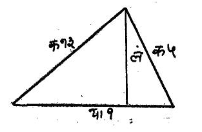
\includegraphics[scale=0.75]{graphics/Capture27.png}\\
\end{center}

\vspace{-4mm}
\noindent अत्र भूमेर्यावत्तावत्कल्पने क्रिया प्रसरति मध्यमाहरणं विना न निर्वहति च~। तथाहि\textendash \,भूमिः या १~। अथ {\qt 'त्रिभुजे भुजयोर्योगः'} इत्यादिनाबाधे यथा~। भुजौ क १३~। क ५~। अनयोर्योगः क १३ क ५ भुजयोरन्तरेणानेन क १३ क ५ं~। \\

\vspace{-2mm}
 गुणनार्थं न्यस्तः $\begin{matrix}
\vspace{-1mm}
\mbox{{क १३~। क १३ क ५}}\\
\vspace{-1mm}
\mbox{{क ~५ं~। क १३ क ५}}
\vspace{1mm}
\end{matrix}$\\
\vspace{-2mm}

 गुणने जातानि करणीखण्डानि क १६९~। क ६५~। क ६ं५~। क २ं५~। अत्र 
मध्यमकरण्योर्धनर्णयोस्तुल्यत्वान्नाशः~। आद्यान्त्यकरण्योर्मूले रू १३ रू
५ं अनयोर्योगे जातं 
गुणनफलं रू ८~। अयं भुवा हृतः $\begin{matrix}
\vspace{-1mm}
\mbox{{रू ८}}\\
\vspace{-1mm}
\mbox{{या १}}
\vspace{1mm}
\end{matrix}$ लब्ध्या समच्छेदेन भूरूनयुता दलिता च
जाते आबाधे $\begin{matrix}
\vspace{-1mm}
\mbox{{याव १ रू ८ं}}\\
\vspace{-1mm}
\mbox{{या २ ~~~~}}
\vspace{1mm}
\end{matrix}$~। $\begin{matrix}
\vspace{-1mm}
\mbox{{याव १ रू ८}}\\
\vspace{-1mm}
\mbox{{या २ ~~~~}}
\vspace{1mm}
\end{matrix}$~। लघोराबाधाया वर्गं $\begin{matrix}
\vspace{-1mm}
\mbox{{यावव १ याव १ं६ रू ६४}}\\
\vspace{-1mm}
\mbox{{याव ४}}
\vspace{1mm}
\end{matrix}$ लघुभुजस्य क ५ वर्गात् रू ५ समच्छेदेनापास्य $\begin{matrix}
\vspace{-1mm}
\mbox{{यावव १ं याव ३६ रू ६४ं}}\\
\vspace{-1mm}
\mbox{{याव ४}}
\vspace{1mm}
\end{matrix}$ जातो लम्बवर्गः~। एवं द्वितीयाबाधावर्गं $\begin{matrix}
\vspace{-1mm}
\mbox{{यावव १ याव १६ रू ६४}}\\
\vspace{-1mm}
\mbox{{याव ४}}
\vspace{1mm}
\end{matrix}$ द्वितीयभुजं क १३ वर्गात् रू १३ समच्छेदेनापास्य वा जातो लम्बवर्गः स एव~। $\begin{matrix}
\vspace{-1mm}
\mbox{{यावव १ं याव ३६ रू ६ं४}}\\
\vspace{-1mm}
\mbox{{याव ४}}
\vspace{1mm}
\end{matrix}$ अथ प्रकारान्तरेण लम्बगुणं भूम्यर्धं क्षेत्रफलं भवतीति व्यस्तविधिना भूम्यर्धेन
 \newpage%%%%%%%%%%%%%%%%%%%%%%%%%%%%%%%%%%
\noindent या $\begin{matrix}
\vspace{-1mm}
\mbox{{१}}\\
\vspace{-1mm}
\mbox{{२}}
\vspace{1mm}
\end{matrix}$ क्षेत्रफलं ४ भक्तं जातो लम्बः $\begin{matrix}
\vspace{-1mm}
\mbox{{रू ८}}\\
\vspace{-1mm}
\mbox{{या १}}
\vspace{1mm}
\end{matrix}$ अस्य वर्गः $\begin{matrix}
\vspace{-1mm}
\mbox{{रू ६४}}\\
\vspace{-1mm}
\mbox{{आव १}}
\vspace{1mm}
\end{matrix}$~। लम्बवर्गयोर्न्यासः 
\vspace{-2mm}

\begin{table}[h!]
    \centering\s
    \begin{tabular}{l}
      यावव १ं  याव ३६ रू ६४\\
 याव ४ \\
 यावव ० याव ० रू ६४ \\
 याव १ 
    \end{tabular}
\end{table}
\vspace{-2mm}

\noindent पक्षौ समच्छेदीकृत्य च्छेदगमे न्यासः 

\vspace{-2mm}
\begin{table}[h!]
    \centering\s
    \begin{tabular}{cccccc}
     यावव& १ं& याव& ३६& रू& ६ं४\\
 यावव& ०& याव& ०& रू& २५६
    \end{tabular}
\end{table}
\vspace{-2mm}

\noindent समशोधने जातं $\begin{matrix}
\vspace{-1mm}
\mbox{{रू ३२ं० ~~~~~~}}\\
\vspace{-1mm}
\mbox{{यावव १ याव ३ं६}}
\vspace{1mm}
\end{matrix}$ अथाव्यक्तवर्गादि यदावशेषमित्यादिवक्ष्यमाणमध्यमाहरणविधिना
पक्षयोरष्टादशवर्गं ३२४ प्रक्षिप्य गृहीते मूले~। $\begin{matrix}
\vspace{-1mm}
\mbox{{~~~~~ रू २}}\\
\vspace{-1mm}
\mbox{{याव १ रू १ं८}}
\vspace{1mm}
\end{matrix}$ अव्यक्तपक्षर्णगरूपतोऽल्पमित्यादिना 
जातं द्विविधं यावत्तावद्वर्गमानं २०~। १६~। अत्राद्यमनुपपन्नत्वान्न
ग्राह्यम्~। अनुपपत्तावुपपत्तिं तु मध्यमाहरणविवरणे वक्ष्यामः~। यावत्तावद्वर्गमानस्य १६
पदं ४ जातं यावत्तावन्मानम्~। इयमेव भूः ४~। अथ पूर्वसिद्धलम्बवर्गं $\begin{matrix}
\vspace{-1mm}
\mbox{{यावव १ं याव ३६ रू ६ं४}}\\
\vspace{-1mm}
\mbox{{याव ४}}
\vspace{4mm}
\end{matrix}$ भूम्यर्धवर्गेण याव $\begin{matrix}
\vspace{-1mm}
\mbox{{१}}\\
\vspace{-1mm}
\mbox{{४}}
\vspace{1mm}
\end{matrix}$ सङ्गुण्य जातः क्षेत्रफलवर्गः $\begin{matrix}
\vspace{-1mm}
\mbox{{यावव १ं याव ३६ रू ६ं४}}\\
\vspace{-1mm}
\mbox{{१६}}
\vspace{4mm}
\end{matrix}$ अयं क्षेत्रफलस्यास्य ४ वर्गेण सम इति समशोधनार्थं न्यासः $\begin{matrix}
\vspace{-1mm}
\mbox{{यावव १ं याव ३६ रू ६ं४}}\\
\vspace{-1mm}
\mbox{{१६}}\\
\vspace{-1mm}
\mbox{{यावव ० याव ० रू १६}}
\vspace{4mm}
\end{matrix}$ पक्षौ समच्छेदीकृत्य च्छेदगमे प्राग्वल्लब्धं यावत्तावन्मानं ४~। तदेवं भूमेर्यावत्तावत्कल्पने क्रिया प्रसरति~। अत आचार्येणाव्यक्तकल्पनानिरपेक्षम् एव
यथोदाहरणसिद्धिर्भवेत्तथा
\newpage
%%%%%%%%%%%%%%%%%%%%%%%%%%%%%%%%%%%%%%

\noindent स्वेच्छयैको भुजो क १३ भूमिः कल्पिता फले विशेषाभावात्~। दर्शनं~। 
\begin{table}[h!]
    \centering\s
    \begin{tabular}{lllll}
       \multirow{7}{*}{क्षेत्रफलं रू ४ } &&\multirow{7}{*}{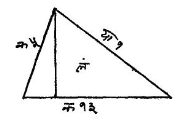
\includegraphics[scale=0.8]{graphics/Capture32.png}}& &\multirow{7}{*}{लम्बः क $\begin{matrix}
\vspace{-1mm}
\mbox{{६४}}\\
\vspace{-1mm}
\mbox{{१३}}
\vspace{1mm}
\end{matrix}$}\\
 &&&&\\
 &&&&\\
 &&&&\\
&&&&\\
&&&&\\
&&&&\\
    \end{tabular}
\end{table}

\noindent लम्बगुणं भूम्यर्धं क्षेत्रफलं भवतीति क्षेत्रफलं भूम्यर्धभक्तं लम्बः
स्यात्~। तत्र यद्यपि द्वाभ्यां भागेऽर्धं भवतीति भूमेरर्धार्थं द्वाभ्यां भाग उचितस्तथापि
वर्गेण वर्गं भजेदित्युक्तत्वात्प्रकृते वर्गरूपाया भूमेरर्धार्थं चतुर्भिरेव भाग उचितः~।
एवं जातं भूम्यर्धं क $\begin{matrix}
\vspace{-1mm}
\mbox{{१३}}\\
\vspace{-1mm}
\mbox{{४}}
\vspace{1mm}
\end{matrix}$~। उक्तवत्क्षेत्रफलमपि वर्गीकृतं क १६~। क्षेत्रफलेऽस्मिन् क १६
भूम्यर्धेनानेन क $\begin{matrix}
\vspace{-1mm}
\mbox{{१३}}\\
\vspace{-1mm}
\mbox{{४}}
\vspace{1mm}
\end{matrix}$ भक्ते जातो लम्बः क $\begin{matrix}
\vspace{-1mm}
\mbox{{६४}}\\
\vspace{-1mm}
\mbox{{१३}}
\vspace{1mm}
\end{matrix}$~। अस्य कोटिरूपवर्गं रू $\begin{matrix}
\vspace{-1mm}
\mbox{{६४}}\\
\vspace{-1mm}
\mbox{{१३}}
\vspace{1mm}
\end{matrix}$ ज्ञातभुजस्य कर्णरूपस्य क ५
वर्गात् रू ५ अपास्य रू $\begin{matrix}
\vspace{-1mm}
\mbox{{१}}\\
\vspace{-1mm}
\mbox{{१३}}
\vspace{1mm}
\end{matrix}$ मूलं क $\begin{matrix}
\vspace{-1mm}
\mbox{{१}}\\
\vspace{-1mm}
\mbox{{१३}}
\vspace{1mm}
\end{matrix}$ जाता लघुराबाधा~। यथा करण्या वर्गे
तत्तुल्यानि रूपाणि भवन्ति तथा रूपाणां मूले रूपतुल्या करणी भवितुमर्हति~। यतो
यस्य राशेर्यो वर्गस्तस्य स राशिर्मूलमिति~। अथाबाधां क $\begin{matrix}
\vspace{-1mm}
\mbox{{१}}\\
\vspace{-1mm}
\mbox{{१३}}
\vspace{1mm}
\end{matrix}$ भूमेः क १३ अपास्य
योगं करण्योरित्यादिना लघ्व्या हृतायास्त्वित्यादिना वा जातान्याबाधा क $\begin{matrix}
\vspace{-1mm}
\mbox{{१४४}}\\
\vspace{-1mm}
\mbox{{१३}}
\vspace{1mm}
\end{matrix}$~। इयमाबाधा भुजः~। लम्बः कोटिः~। अज्ञातभुजः कर्णः~। अत्र भुजकोट्योर्ज्ञाने तत्कृत्यार्योगपदं कर्ण इति कर्णः सुलभः~। द्वितीयाबाधायाः क $\begin{matrix}
\vspace{-1mm}
\mbox{{१४४}}\\
\vspace{-1mm}
\mbox{{१३}}
\vspace{1mm}
\end{matrix}$ वर्गः रू $\begin{matrix}
\vspace{-1mm}
\mbox{{१४४}}\\
\vspace{-1mm}
\mbox{{१३}}
\vspace{1mm}
\end{matrix}$ लम्बस्य क $\begin{matrix}
\vspace{-1mm}
\mbox{{६४}}\\
\vspace{-1mm}
\mbox{{१३}}
\vspace{1mm}
\end{matrix}$ वर्गेण रू $\begin{matrix}
\vspace{-1mm}
\mbox{{६४}}\\
\vspace{-1mm}
\mbox{{१३}}
\vspace{1mm}
\end{matrix}$ युतः रू १६~। अस्य पदं रू ४ ज्ञातोऽज्ञातभुजः~।
प्रष्ट्रा या भूमिः पृष्टा सैवाचार्येण भुजत्वेन कल्पिता~। तस्मादत्र यो भुजोऽवगतः रू
४ इय-

\newpage%%%%%%%%%%%%%%%%%%%%%%%%%%%%%%%%%%

\noindent मेव सा भूः~। एवमन्यं भुजं क ५ भूमिं प्रकल्प्य न्यासः 
\begin{table}[h!]
    \centering\s
    \begin{tabular}{lllll}
       \multirow{7}{*}{क्षेत्रफलं रू ४ } &&\multirow{7}{*}{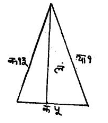
\includegraphics[scale=0.85]{graphics/Capture31.png}}& &\multirow{7}{*}{लम्बः क $\begin{matrix}
\vspace{-1mm}
\mbox{{६४}}\\
\vspace{-1mm}
\mbox{{५}}
\vspace{1mm}
\end{matrix}$}\\
 &&\\
 &&\\
 &&\\
 &&\\
 &&\\
 &&\\
    \end{tabular}
\end{table}

\noindent अत्रापि पूर्ववत्फलाल्लम्बः क $\begin{matrix}
\vspace{-1mm}
\mbox{{६४}}\\
\vspace{-1mm}
\mbox{{५}}
\vspace{1mm}
\end{matrix}$~। लम्बवर्गं रू $\begin{matrix}
\vspace{-1mm}
\mbox{{६४}}\\
\vspace{-1mm}
\mbox{{५}}
\vspace{1mm}
\end{matrix}$ भुजवर्गात् रू १३ अपास्य रू $\begin{matrix}
\vspace{-1mm}
\mbox{{१}}\\
\vspace{-1mm}
\mbox{{५}}
\vspace{1mm}
\end{matrix}$ मूलं क $\begin{matrix}
\vspace{-1mm}
\mbox{{१}}\\
\vspace{-1mm}
\mbox{{५}}
\vspace{1mm}
\end{matrix}$ जाताबाधा~। इमां योगं करण्योरित्यादिना भूमेः क ५ अपास्य
जातान्या क $\begin{matrix}
\vspace{-1mm}
\mbox{{१६}}\\
\vspace{-1mm}
\mbox{{५}}
\vspace{1mm}
\end{matrix}$~। अस्या वर्गात् रू $\begin{matrix}
\vspace{-1mm}
\mbox{{१६}}\\
\vspace{-1mm}
\mbox{{५}}
\vspace{1mm}
\end{matrix}$ लम्बवर्गेण रू $\begin{matrix}
\vspace{-1mm}
\mbox{{६४}}\\
\vspace{-1mm}
\mbox{{५}}
\vspace{1mm}
\end{matrix}$ युतात् १६ मूलं ज्ञातोऽज्ञातभुजः ४~। 
एवमन्यथापि सुधीभिरूह्यम्~॥~१०४~॥~\\

\vspace{-2mm}
 अथान्यदुदाहरणमार्ययाह\textendash
 \begin{quote}
     \eg
    दशपञ्चकरण्यन्तरमेको बाहुः परश्च षट् करणी~। \\
 भूरष्टादश करणी रूपोना लम्बमाचक्ष्व~॥~१०५~॥~ 
 \end{quote}

 स्पष्टोऽर्थः~। अत्राबाधाज्ञाने लम्बज्ञानमिति लघुराबाधा कल्पिता या १~। एतदूना भूरन्याबाधेति तथा न्यासः 
\begin{figure}[h!]
    \centering
    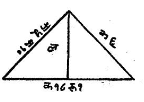
\includegraphics[scale=0.8]{graphics/Capture30.png}
\end{figure}
\newpage
%%%%%%%%%%%%%%%%%%%%%%%%%%%%%%%%%%%%%%%%%%%%%%%

\noindent अत्राबाधे भुजौ~। भुजौ तु कर्णौ~। कोटिस्तूभयत्र लम्ब एवेति
स्वाबाधावर्गं स्वभुजवर्गादपास्य लम्बवर्गौ भवतः~। तत्र लघोराबाधाया वर्गः याव १~। लघुभुजस्यास्य क
५ं क १ 
स्थाप्योऽन्त्यवर्गश्चतुर्गुणान्त्यनिघ्ना इत्यादिना क २५ क २०ं० क १००
आद्यान्त्यकरण्योर्योगे कृते क २२५ मूले च गृहीते रू १५ जातो लघुभुजवर्गः रू १५ क २०ं०
अयमाबाधावर्गोनः च सञ्जातो लम्बवर्गः याव १ं रू १५ क २०ं०~। एवं
द्वितीयाबाधायाः 
या १ रू १ क १८~। यत्र {\qt स्थाप्योऽन्त्यवर्गः} इत्यादिना यथासम्भवं
द्विगुणान्त्यनिघ्नाश्चतुर्गुणान्त्यनिघ्नाश्चेति कृते जातो वर्गः याव १ या २ याक ७२ रू
१ क ७ं२ 
क ३२४~। अन्त्यकरण्या मूलं रू १८ रुपेण संयोज्य परखण्डानां
भिन्नजातित्वात् 
पृथक्स्थितौ च जातः याव १ या २ याक ७ं२ रू १९ क ७ं२~। एवमाबाधावर्गं 
स्वभुजस्यास्य क ६ वर्गादस्मात् रू ६ विशोध्य वा जातो लम्बवर्गं याव १ं
या २ं याक 
७२ रू १ं३ क ७२  लम्बवर्गौ समाविति समशोधनार्थं न्यासः 

\begin{table}[h!]
    \centering\s
    \begin{tabular}{l}
        याव १ं या ० याक ० ~रू १५ क २०ं० \\
	    याव १ं या २ं याक ७२ रू १ं३ ~क ७२ 
    \end{tabular}
\end{table}
\vspace{-2mm}

\noindent अत्राद्यपक्षादव्यक्तमात्रे \,शोधित \,इतरस्माच्च \,व्यक्तमात्रे \,शोधिते \,योगं \,करण्योरित्यादिना करण्योर्योगे च कृते जाते शेषे $\begin{matrix}
\vspace{-1mm}
\mbox{{या ~२ याक ७ं२}}\\
\vspace{-1mm}
\mbox{{रू २८ं क ५१२}}
\vspace{1mm}
\end{matrix}$ अथाव्याक्तशेषेण व्यक्तशेषस्य भागार्थं न्यासः~। $\begin{matrix}
\vspace{-1mm}
\mbox{{रू २ं८ क ५१२}}\\
\vspace{-1mm}
\mbox{{या २ याक ७ं२}}
\vspace{1mm}
\end{matrix}$ अत्राव्यक्तशेषेण व्यक्तशेषं कथं भाज्यमित्याह {\qt 'अत्र याकारस्य प्रयोजनाभावात्तदपगमे कृते समभाज्यभाजकौ'} इति $\begin{matrix}
\vspace{-1mm}
\mbox{{रू २ं८ क ५१२}}\\
\vspace{-1mm}
\mbox{{रू ~२ ~क ७ं२}}
\vspace{1mm}
\end{matrix}$~। वस्तुतस्त्वव्यक्तशेषतुल्येनाव्यक्तेन यदि
व्यक्तशेषं तुल्यं व्यक्तं लभ्यते तदैकेनाव्यक्तेन किमिति त्रैराशिकेन 
\vspace{-4mm}

\begin{table}[h!]
    \centering\s 
    \begin{tabular}{l}
        या २ याक ७ं२~। रू २८ं क ५१२~। या १ 
\end{tabular}
\end{table}
\vspace{-2mm}

\noindent अव्यक्तस्य व्यक्तं मानं भवतीतीच्छाप्रमाणयोर्यावत्तावतापवर्ते
भवतीष्टो हरः रू २ क ७ं२~। अन्यथान्यत्राप्यव्यक्तशेषेण रूपशेषे भक्ते रूपात्मकं फलं कथं स्यात्~। आचार्यैस्त्वन्यत्र याकारस्यापगमेऽप्यज्ञानां गणितसिद्धिर्भवतीति तत्र
याकारापगमो नोक्तः~। प्रकृते तु याकारनपगमे 'धनर्णताव्यत्ययमीप्सितायाश्छेदे करण्याः' इत्यादिना भाज्यभाजकयोर्गुणने भूयाननर्थः स्यादिति याकारापगम उक्तः~। अथ द्विसप्ततिमिताया
\newpage
%%%%%%%%%%%%%%%%%%%%%%%%%%%%%%%%%%
\noindent भाजककरण्या धनत्वं प्रकल्प्य तादृक्छिदा क ४ क ७२ भाज्यभाजकयोर्गुणनार्थे न्यासः 
\vspace{2mm}

\begin{tabular}{lll}
    क ~४~। &क ७८ं४ क ५१२~। & क ~४~। ~~क ४ ~~क ७ं२ \\
 क ७२~। &क ७८ं४ &क ५१२~। क ७२~। क ७ं२ 
\end{tabular}
\vspace{2mm}

\noindent भाज्ये गुणिते जातानि खण्डानि ~क ३१ं३६ ~क २०४८ ~क ५६४ं४८ ~क ३६८६४~। \\
\vspace{-4mm}

\noindent अत्राद्यान्त्ययोर्द्वितीयतृतीययोश्च करण्योर्लघ्व्या हृतायास्तु
पदमित्यादिनान्तरे कृते जाते 
भाज्यकरण्यौ क १८४९६ क ३६९ं९२~।\\

\vspace{-4mm}
 एवं भाजके करणीखण्डानि ~क १६ ~क २८ं८ ~क २८८ ~क ५१ं८४~। \\

\vspace{-4mm}
 अत्र द्वितीयतृतीयकरण्योरन्तरे नाशः~। आद्यान्त्ययोरन्तरे कृते जाता
भाजककरणी 
क ४६ं२४~। अनया भाज्ये हृते लब्धं यावत्तावन्मानं क ४ं क ८~। प्रथमकरण्या मूले गृहीते जातं रू २ं क ८~। इयमेव लघुराबाधा~। एतदूना भूः 
रू १ं क १८ योगं करण्योरित्यन्तरे कृते जाता द्वितीयाबाधा रू १ क २~।\\

\vspace{-4mm}
 अथ प्रथमलम्बवर्गस्योत्थापनार्थं न्यासः याव १ं रू १५ क २०ं०~। 
अत्राद्यमेव खण्डमव्यक्तं स च यावद्वर्गोऽस्ति~। अतो
यावत्तावन्मानस्यास्य क ४ं 
क ८ वर्गो रू १२ क १२ं८ जातं यावत्तावद्वर्गमानम्~। यावद्वर्गस्य
ऋणगतत्वादिदं 
रू १२ क १२ं८ उत्तरखण्डद्वयादस्मात् रू १५ क २०ं० विशोध्य जातो 
लम्बवर्गः रू ३ क ८ं~। एवं द्वितीयस्य लम्बवर्गस्योत्थापनार्थं न्यासः
\begin{table}[h!]
    \centering\s
    \begin{tabular}{l}
      याव १ं ~या २ं ~याक ७२ ~रू १३ ~क ७२~। 
    \end{tabular}
\end{table}
\vspace{-2mm}

 अत्राद्यं खण्डत्रयम् अव्यक्तम्~। तत्र प्रथमखण्डस्य पूर्ववन्मानं रू १२ क
१२ं८~। द्वितीयखण्डे यावत्तावद्द्वयमस्तीति यावत्तावन्मानं रू २ं  क ८
द्वाभ्यां सङ्गुण्य वर्गेण वर्गं गुणयेदिति करणीं चतुर्भिः सङ्गुण्य जातं द्वितीयखण्डमानं रू ४ं क ३२~। अथ तृती-यस्य~। यद्येकेन यावत्तावता व्यक्तमानमिदं क ४ं क ८
तदभीष्टेनानेन याक ७२ किमिति त्रैराशिकार्थं न्यासः~। या १~। क ४ं क ८~। याक ७२~। \\

\vspace{-4mm}
 अत्र प्रमाणेच्छयोः प्रमाणेनापवर्ते कृतेऽपवर्तितेच्छया क ७२ फले गुणिते जातं 
तृती-यखण्डमानं क २८ं८ क ५७६~। द्वितीयकरण्या मूले गृहीते जातं रू २४ क
\newpage
%%%%%%%%%%%%%%%%%%%%%%%%%%%%%%%%%%%%%
\noindent २८ं८~। एवं जातान्यव्यक्तखण्डत्रयस्य व्यक्तमानानि \\

\vspace{-4mm}
\hspace{6mm} रु १२ क १२ं८~। रू ४ं क ३२~। रू २४ क २८ं८~। \\

\vspace{-4mm}
 अत्र लम्बवर्गे आद्ययोरव्यक्तखण्डयोर्ऋणत्वेन
शोध्यत्वात्तदुत्थव्यक्तयोरपि शोध्यत्वेन संशोध्यमानं स्वमृणत्वमेतीत्यादिना जातं रू १ं२  क १२८~। रू ४ क ३ं२~। रू २४ क २८ं८~। एवमग्रिमव्यक्तद्वयेन सह जातानि पञ्च खण्डानि लम्बवर्गे\\

\vspace{-4mm}
\hspace{6mm} रु १ं२ क १२८~। रू ४ क ३ं२~। रू २४ क २८ं८~। रू १ं३~। क ७२~।\\

\vspace{-4mm}
 अत्र रूपाणां यथोक्तयोगे कृते जातं रू ३~। आद्ययोः करण्योः क १२८ 
क ३ं२ अन्तरे \,जातं \,क ३२~। अस्या \,तृतीयकरण्या \,सह २८ं८ \,अन्तरे \,जातं \,क १२ं८~। अस्याः पुनरन्त्यया क ७२ अन्तरे जातं क ८ं~। अथवा ऋणकरण्योरनयोः क ३२ क २८८ धनकरण्योरनयोश्च क १२८ क ७२ योगे 
जातं करणीद्वयं क ५१२~। क ३९२~। अनयोरन्तरे जाता सैव करणी क ८ं~। 
एवं जातो लम्बवर्गः स एव रू ३ क ८ं~। अथवाबाधा क ४ं क ८ वर्गं रू
१२ क १२ं८ स्वभुजस्य क ५ं क १० वर्गात् रू १५ क २०ं० उक्तवदपास्य
जातो लम्बवर्गः स एव रू ३ क ८ं~। एवं द्वितीयाबाधा क १ क २ वर्गं रू 
३ क ८ स्वभुजं क ६ वर्गात् रू ६ अपास्य जातो लम्बवर्गः स एव रू ३ क
८ं~। \\

\vspace{-4mm}
 अथास्य पदम्~। तत्र ऋणात्मिका चेत्करणी कृतौ स्याद्धनात्मिकां तां परिकल्प्येति कृते रूपकृतेः ९ करणीतुल्यानि रूपाणि ८ अपास्य शेषस्य १ पदेन १
रूपाणि 
३ युतोनितानि ४~। २~। अर्धे २~। १~। ऋणात्मिकैका सुधियावगम्येत्यल्पकरण्या ऋणत्वे कृते पदे च गृहीते जातो लम्बः रू १ं क २~। इदमुदाहरणं 
व्यक्तमार्गेणापि सिध्यति~। तद्यथा\textendash \,त्रिभुजे भुजयोर्योग इत्यादिना
भुजयोरनयोः क ५ं क १०~। क ६~। योगः क ५ं क १० क ६~। लघुभुजं क ५ं क १० महतो भुजात् क ६ अपास्य जातं भुजयोरन्तरं क ५ क १ं० क ६~। अन्तरेण योगस्य गुणनार्थं न्यासः~। 
\begin{table}[h!]
    \centering\s
    \begin{tabular}{lrlrlrlr}
     क &५~। &क &५ं&क &१० &क &६ \\
 क &१ं०~।& क &५ं& क& १०& क& ६\\
 क &६~। &क &५ं &क &१० &क& ६
    \end{tabular}
\end{table}

\newpage
%%%%%%%%%%%%%%%%%%%%%%%%%%%%%%%%%%
\noindent गुणिते जातं खण्डनवकं 
\begin{table}[h!]
    \centering\s
    \begin{tabular}{l}
        क २५ं ~क ५० ~क ३० ~क ५० ~क १०ं० ~क ६ं० ~क ३ं० ~क ६० ~क ३६ 
    \end{tabular}
\end{table}
\vspace{-2mm}

 अत्र त्रिंशन्मितकरण्योः षष्टिमितकरण्योश्च धनर्णत्वान्नाशे
पञ्चाशन्मितकरण्योर्योगे च कृते क २०० शेषकरणीमूलानां ५ं~। १ं०~। ६ योगे च कृते ९ं जातं गुणनफलं रू ६ं क २०० इदं भूम्यानया रू १ं क १८ भाज्यम्~। अत्र वर्गेण वर्गं भजेदित्युक्तेः क्षयो भवेच्च क्षयरूपवर्ग इति रूपवर्गे कृते जातौ
भाज्यभाजकौ $\begin{matrix}
\vspace{-1mm}
\mbox{{क ८ं१ ~क २००}}\\
\vspace{-1mm}
\mbox{{क ~१ं ~क ~१८}}
\vspace{1mm}
\end{matrix}$~।\\

 अथ भाजकस्यैकीकरणार्थं धनर्णताव्यत्ययमीप्सिताया इत्यादिना भाजककरण्याः 
क १ं धनत्वं प्रकल्प्य तादृक्छिदा क १ क १८ भाज्यभाजकयोर्गुणनार्थं न्यासः 
\begin{table}[h!]
    \centering\s
    \begin{tabular}{lrllllrllll}
      क &१ ~। &क ८ं१& क &२००& क& १ ~।& क& १ं& क &१८ \\
 क &१८ ~। &क ८ं१& क& २००& क& १८ ~।& क& १ं& क &१८ 
    \end{tabular}
\end{table}
 
 भाज्ये गुणिते जातानि करणीखण्डानि क ८ं१ क २०० क १४ं५८
क ३६०० आद्यान्त्यकरण्योर्मध्यमकरण्योश्चान्तरे जातो भाज्यः क २६०१ क
५७ं८~। भाजके गुणिते जातं क १ं क १८ क १ं८ क ३२४~। मध्यमकरण्योर्नाशे
आद्यान्त्यकरण्योरन्तरे कृते जाता भाजक एकैव करणी क २८६~। अनया भाज्ये भक्ते लब्धिः क १ क २ं~। प्रथमकरण्या पदे जाता लब्धिः रू ३ क २ं~। अनया भूरेषा रू १ं क १८ यथावदूनयुता~। रू ४ं क ३२~। रू २ क ८~। यथावदर्द्धिता रू २ं क ८~। रू १ क २ जाते आबाधे~। आभ्यां पूर्ववल्लम्बः रू १ं क २~।
आसन्नमूलग्रहणेन जाता क्षेत्रभुजाद्याः~। दर्शनं 
\vspace{-2mm}

\begin{figure}[h!]
    \centering
    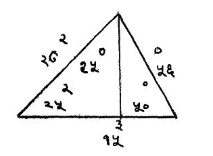
\includegraphics[scale=0.8]{graphics/Capture29.png}
\end{figure}
\newpage
%%%%%%%%%%%%%%%%%%%%%%%%%%%%%%%%%%%%%%%%%%
 अत्र दशपञ्चकरण्योरासन्नमूले~। ३~। १०~॥ २~। १४~। अनयोरन्तरमेको भुजः ०~। ५६~। एवं सर्वत्र द्रष्टव्यम्~। अत्रापि प्रतीत्यर्थं गणितं लिख्यते~। भुजयोः $\begin{matrix}
\vspace{-1mm}
\mbox{{०}}\\
\vspace{-1mm}
\mbox{{५६}}
\vspace{1mm}
\end{matrix}$~। $\begin{matrix}
\vspace{-1mm}
\mbox{{२}}\\
\vspace{-1mm}
\mbox{{२७}}
\vspace{1mm}
\end{matrix}$~। योगः $\begin{matrix}
\vspace{-1mm}
\mbox{{३}}\\
\vspace{-1mm}
\mbox{{२३}}
\vspace{1mm}
\end{matrix}$~। भुजयोरन्तरेण $\begin{matrix}
\vspace{-1mm}
\mbox{{१}}\\
\vspace{-1mm}
\mbox{{३१}}
\vspace{1mm}
\end{matrix}$ गुणितः $\begin{matrix}
\vspace{-1mm}
\mbox{{५}}\\
\vspace{-1mm}
\mbox{{८}}
\vspace{1mm}
\end{matrix}$ भुवा $\begin{matrix}
\vspace{-1mm}
\mbox{{३}}\\
\vspace{-1mm}
\mbox{{१५}}
\vspace{1mm}
\end{matrix}$ हृतो लब्धिः $\begin{matrix}
\vspace{-1mm}
\mbox{{१}}\\
\vspace{-1mm}
\mbox{{३५}}
\vspace{1mm}
\end{matrix}$ अनया द्विष्टा भूरूनयुता $\begin{matrix}
\vspace{-1mm}
\mbox{{१}}\\
\vspace{-1mm}
\mbox{{४०}}
\vspace{1mm}
\end{matrix}$~। $\begin{matrix}
\vspace{-1mm}
\mbox{{४}}\\
\vspace{-1mm}
\mbox{{५०}}
\vspace{1mm}
\end{matrix}$ दलिता जाते आबाधे $\begin{matrix}
\vspace{-1mm}
\mbox{{०}}\\
\vspace{-1mm}
\mbox{{५०}}
\vspace{1mm}
\end{matrix}$~। $\begin{matrix}
\vspace{-1mm}
\mbox{{२}}\\
\vspace{-1mm}
\mbox{{२५}}
\vspace{1mm}
\end{matrix}$~। अथाबाधा $\begin{matrix}
\vspace{-1mm}
\mbox{{०}}\\
\vspace{-1mm}
\mbox{{५०}}
\vspace{1mm}
\end{matrix}$ वर्गं $\begin{matrix}
\vspace{-1mm}
\mbox{{०}}\\
\vspace{-1mm}
\mbox{{४२}}
\vspace{1mm}
\end{matrix}$ स्वभुज\textendash \,$\begin{matrix}
\vspace{-1mm}
\mbox{{०}}\\
\vspace{-1mm}
\mbox{{५६}}
\vspace{1mm}
\end{matrix}$\textendash \,वर्गात् $\begin{matrix}
\vspace{-1mm}
\mbox{{०}}\\
\vspace{-1mm}
\mbox{{५२}}
\vspace{1mm}
\end{matrix}$ अपास्य शेषस्य $\begin{matrix}
\vspace{-1mm}
\mbox{{०}}\\
\vspace{-1mm}
\mbox{{१०}}
\vspace{1mm}
\end{matrix}$ मूलं $\begin{matrix}
\vspace{-1mm}
\mbox{{०}}\\
\vspace{-1mm}
\mbox{{२५}}
\vspace{1mm}
\end{matrix}$ जातो लम्बः~। एवं द्वितीयाबाधा $\begin{matrix}
\vspace{-1mm}
\mbox{{२}}\\
\vspace{-1mm}
\mbox{{२५}}
\vspace{1mm}
\end{matrix}$ वर्गं $\begin{matrix}
\vspace{-1mm}
\mbox{{५}}\\
\vspace{-1mm}
\mbox{{५०}}
\vspace{1mm}
\end{matrix}$ स्वभुज\textendash \,$\begin{matrix}
\vspace{-1mm}
\mbox{{२}}\\
\vspace{-1mm}
\mbox{{२७}}
\vspace{1mm}
\end{matrix}$\textendash \,वर्गात् ६ अपास्य शेषस्य $\begin{matrix}
\vspace{-1mm}
\mbox{{०}}\\
\vspace{-1mm}
\mbox{{१०}}
\vspace{1mm}
\end{matrix}$ मूलं $\begin{matrix}
\vspace{-1mm}
\mbox{{०}}\\
\vspace{-1mm}
\mbox{{२५}}
\vspace{1mm}
\end{matrix}$ जातो लम्बः स एव $\begin{matrix}
\vspace{-1mm}
\mbox{{०}}\\
\vspace{-1mm}
\mbox{{२५}}
\vspace{1mm}
\end{matrix}$~। एवमन्यत्रापि सुधीभिरूह्यम्~॥~१०५~॥ \\

 अथ पक्षयोः समशोधनानन्तरमव्यक्तवर्गघनादिकेऽपि शेषे यथासम्भवमपवर्तेन
मध्यमाहरणं विनैवोदाहरणसिद्धिरस्तीति प्रदर्शयितुमुदाहरणषट्कमाह~।
तत्रोदाहरणद्वयमनुष्टु-भाह\textendash

\begin{quote}
    \eg
      असमानसमच्छेदान् राशींस्तांश्चतुरो वद~। \\
 यदैक्यं यद्धनैक्यं वा येषां वर्गैक्यसम्मितम्~॥~१०६~॥
\end{quote}

असमानाश्च ते समच्छेदाश्च तान्~। यदैक्यं येषां वर्गैक्यसम्मितमित्येकं
यद्धनैक्यं येषां वर्गैक्यसम्मितमिति द्वितीयमित्युदाहरणद्वयम्~।
असमानसमप्रज्ञेति पाठे तु हे असमप्रज्ञ 
निरुपमबुद्धे समास्ताश्चतुरो राशीन्वदेति योजनीयम्~।
प्रथमपाठस्त्वसाधुरिति प्रतिभाति 
न हि समच्छेदत्वपुरस्कारेणोदाहरणमिह साध्यते किं तु समच्छेदत्वं
सम्पातायातम्~। 
असमानिति त्वपेक्षितमेव~। अन्यथा रूपमितैश्चतुर्भिरुदाहरणसिद्धेः~। अत्र
राशीनामसमानत्वेनोद्देशात्कल्पिता अतुल्या राशयः~। या १ या २ या
३ या ४ 
उदाहरणद्वयस्यापि गणितं त्वाकर एव स्फुटम्~॥~१०६~॥~\\

\vspace{-2mm}
 अन्यदुदाहरणद्वयमनुष्टुभाह\textendash
\begin{quote}
    \eg 
     त्र्यस्रक्षेत्रस्य यस्य स्यात्फलं कर्णेन सम्मितम्~। \\
 दोःकोटिश्रुतिघातेन समं यस्य च तद्वद~॥~१०७~॥~
\end{quote}

 \newpage%%%%%%%%%%%%%%%%%%%%%%%%%%%%%%%%%%

 स्पष्टोऽर्थः~। अत्र दोःकोटिकर्णानामव्यक्तकल्पने विशेषोऽस्ति~।
जात्यत्र्यस्रे नियतानां 
तेषां बाधितत्वात्~। अत इष्टजात्यस्य भुजकोटिकर्णैः पृथग्गुणितं
यावत्तावत्तेषां 
मानानि प्रकल्प्योदाहरणद्वयमपि साध्यम्~। आकर एव स्पष्टमन्यत्~॥~१०७~॥~\\

\vspace{-2mm}
 अन्यदुदाहरणमनुष्टुभाह\textendash 
 \begin{quote}
     \eg 
युतौ वर्गोऽन्तरे वर्गो ययोर्घाते घनो भवेत्~। \\
 तौ राशी शीघ्रमाचक्ष्व दक्षोऽसि गणिते यदि~॥~१०८~॥~
 \end{quote}
 
 ययो राश्योर्युतावन्तरे च वर्गो भवेद्घाते तु धनो भवेत्तौ राशी शीघ्रं वद~। 
अत्र क्रियासङ्कोचार्थं तथा राशी कल्प्यौ यथा युतावन्तरे च वर्गः स्यात्~।
तथा कल्पितौ 
याव ४ याव ५~। अनयोर्घातो यावव २०~। एष घन इतीष्टयावत्तावद्दशकस्य घनेन
याघ १००० समीकरणे पक्षौ यावत्तावद्घनेनापवर्त्य प्राग्वज्जातौ राशी १००००~। 
१२५००~॥~१०८~॥~\\

\vspace{-2mm}
 अथान्यदुदाहरणमनुष्टुभाह\textendash
\begin{quote}
    \eg 
    घनैक्यं जायते वर्गो वर्गैक्यं च ययोर्घनः~। \\
 तौ चेद्वेत्सि तदाहं त्वां मन्ये बीजविदां वरम्~॥~१०९~॥~
\end{quote}
 
 स्पष्टोऽर्थः~। अत्र यथैक आलापः स्वतः सम्भवति तथा राशी कल्पितौ याव १ 
याव २~। अनयोर्घनयोगः यावघ ९ एष स्वयमेव वर्गो जातः~। यतोऽस्य 
वर्गमूलमिदं याघ ३ अस्मिन्नर्थे आकर एवाक्षिप्य समाहितम्~। अयमर्थः~। 
यावद्वर्गघनो राशिः षट्घातात्मकोऽस्ति~। समद्विघातस्य समत्रिघातो भवतीति
यथा 
द्विघातस्य धनस्तथा त्रिघातस्य समद्विघातो भवतीति त्रिघातस्य वर्गोऽपि
भवितुं युक्त 
एवेति~। अथ तयोरेव राश्योः याव १ याव २ वर्गयोगः यावव ५~। अयं 
घन इतीष्टं यावत्तावत्पञ्चकधनं याध १२५ समं कृत्वा पक्षौ यावत्तावद्घनेनापवर्त्य प्रावग्वजातौ राशी ६२५~। १२५०~। अथवान्यथा मया कल्पितौ राशी 
याघ ५ याघ १० अनयोर्वर्गैक्यं स्वत एव घनो जायते याघव १२५~। अस्य 
षड्घातात्मकत्वाद्द्विघातरूपं घनमूलं यतः सम्भवति याव ५~। अथानयो राश्योः 
याघ ५ याघ १० घनैक्यं याघध ११२५~। एतद्वर्ग इति
यावत्तावद्वर्गवर्गपञ्चसप्ततिः~।
\newpage
%%%%%%%%%%%%%%%%%%%%%%%%%%%%%%%%%%%%%%%%%%%%%
\noindent यावव ७५~। वर्गेण याववव ५६२५ समं कृत्वा पक्षौ
यावत्तावद्वर्गवर्गेणापवर्त्य पक्षयोः न्यासः \;$\begin{matrix}
\vspace{-1mm}
\mbox{{या ११२५ रू ०}}\\
\vspace{-1mm}
\mbox{{या ० रू ५६२५}}
\vspace{1mm}
\end{matrix}$\; पूर्ववद्यावत्तावन्मानं ५~। अनेनोत्थापितौ
राशी तावेव ६२५~। १२५०~। अथवायं याघघ ११२५ वर्ग इति यावत्तावद्वर्गवर्गवर्गवर्गपञ्चकस्य यावववव ५ तत्पञ्चदशकस्य वा यावववव १५ वर्गेण याववववव २५ अनेन वा याववववव २२५ समं कृत्वा पक्षौ याघघ १ अनेनापवर्त्य प्राग्वद्यावत्तावन्मानं ४५ वा ५~। एवमनेकधा~। एवम् अव्यक्तापवर्तनं यथा सम्भवति तथान्यदपि चिन्त्यम्~॥~१०९~॥\\

\vspace{-2mm}
 अथान्यदुदाहरणं गीत्याह\textendash
\begin{quote}
    \eg 
    यत्र त्र्यस्रे क्षेत्रे धात्री मनुसम्मिता सखे बाहू~। \\
 एकः पञ्चदशान्यस्त्रयोदश वदावलम्बकं तत्र~॥~११०~॥
\end{quote}

 स्पष्टोऽर्थः~। आबाधा या १ प्रकल्प्य गणितमप्याकर एव स्फुटम्~।
अनतिप्रयोजनम् एतदुदाहरणम्~॥~११०~॥\\

\vspace{-2mm}
 अथ भुजे कोटिकर्णयोगे च ज्ञाते तयोः पृथक्करणं दर्शयितुमुदाहरणं
मालिन्याह\textendash
\begin{quote}
    \eg
     यदि समभुवि वेणुर्द्वित्रिपाणिप्रमाणो \\
 गणक पवनवेगादेकदेशे सुभग्नः~। \\
 भुवि नृपमितहस्तेष्वङ्ग लग्नं तदग्रं \\
 कथय कतिषु मूलादेष भग्नः करेषु~॥~१११~॥~
\end{quote}

 स्पष्टोऽर्थः~। अत्र वंशाधरखण्डं कोटिस्तत्प्रमाणं या १ प्रकल्प्य
गणितमाकरे 
स्फुटम्~। एवमूर्ध्वखण्डमपि या १ प्रकल्प्य गणितं द्रष्टव्यम्~। एवं कोटौ
भुजकर्णयोगे च ज्ञाते तत् पृथक्करणमपि द्रष्टव्यम्~। \\

\vspace{-2mm}
 तदुदाहरणं पाट्यामुक्तम्~। यथा\textendash
\begin{quote}
    {\qt अस्ति स्तम्भतले बिलं तदुपरि क्रीडाशिखण्डी स्थितः \\
 स्तम्भे हस्तनवोच्छ्रिते त्रिगुणितस्तम्भप्रमाणान्तरे~।}
\end{quote}
\newpage 
%%%%%%%%%%%%%%%%%%%%%%%%%%%%%%%%%%
\begin{quote}
     {\qt दृष्ट्वाहिं बिलमाव्रजन्तमपतत्तिर्यक्स तस्योपरि \\
 क्षिप्रं ब्रूहि तयोर्बिलात्कतिमितैः साम्येन गत्योर्युतिः~॥~}
 
\end{quote}

 अत्रापि भुजं कर्णं वा या १ प्रकल्प्य प्राग्वद्गणितं द्रष्टव्यम्~॥~१११~॥\\
 \vspace{-2mm}
 
 अथ कोटिकर्णान्तरे भुजे च ज्ञाते कोटिकर्णज्ञानं भवतीति
प्रदर्शयितुमुदाहरणं मन्दाक्रान्तयाह\textendash
\begin{quote}
    \eg 
     चक्रक्रौञ्चाकुलितसलिले क्वापि दृष्टं तडागे \\
 तोयादूर्ध्वं कमलकलिकाग्रं वितस्तिप्रमाणम्~। \\
 मन्दं मन्दं चलितमनिलेनाहतं हस्तयुग्मे \\
 तस्मिन्मग्नं गणक कथय क्षिप्रमम्बुप्रमाणम्~॥~११२~॥
\end{quote}

 स्पष्टोऽर्थः~। एतत्क्षेत्रसंस्थानं पाट्यां पाठनिबद्धम्~। यथा\textendash
\begin{quote}
{\qt सखे पद्मतन्मज्जनस्थानमध्यं भुजः कोटिकर्णान्तरं पद्मदृश्यम्~। \\
 नलः कोटिरेतन्मितं स्याद्यदम्भो वदैवं समानीय पानीयमानम्~॥}
\end{quote}
 
 अत्र नलिनीनलप्रमाणं जलगाम्भीर्यम् इति तत्प्रमाणं या १ प्रकल्प्य गणितमाकरे स्फुटम्~॥~११२~॥~\\

\vspace{-2mm}
 अथान्यदुदाहरणं शार्दूलविक्रीडितेनाह\textendash
\begin{quote}
    \eg 
    वृक्षाद्धस्तशतोच्छ्रयाच्छतयुगे वापीं कपिः कोऽप्यगात् \\
 उत्तीर्याथ परो द्रुतं श्रुतिपथात्प्रोड्डीय किञ्चिद्द्रुमात्~। \\
 जातैवं समता तयोर्यदि गतावुड्डीयमानं कियत्\\
 विद्वंश्चेत्सुपरिश्रमोऽस्ति गणिते क्षिप्रं तदाचक्ष्व मे~॥~११३~॥~
\end{quote}
 
 परः कपिर्द्रुमात् किञ्चित् प्रोड्डीय श्रुतिपथाद्वापीमगादिति योजनीयम्~।
श्रुतिपथादिति 
ल्यब्लोपे पञ्चमी~। श्रुतिपथमाश्रित्येति तदर्थः~। शेषं स्पष्टम्~।
अत्रोड्डीयमानं या १ 
प्रकल्प्य गणितमाकरे स्पष्टम्~॥~११३~॥
\newpage
%%%%%%%%%%%%%%%%%%%%%%%%%%%%%%%%%%%
अथान्यदुदाहरणमार्ययाह\textendash
\begin{quote}
    \eg 
     पञ्चदशदशकरोच्छ्रायवेण्वोरज्ञातमध्यभूमिकयोः~। \\
 इतरेतरमूलाग्रगसूत्रयुतेर्लम्बमानमाचक्ष्व~॥~११४~॥~
\end{quote}

 अत्र लम्बज्ञानार्थं वेण्वन्तरालभूमिज्ञानं नावश्यकमिति सूचयितुमज्ञातमध्यभूमिकयोरिति वेणुविशेषणं न तु प्रश्नपूरणार्थम्~। तेन विनापि प्रश्नपूरणात्~। शेषं स्पष्टम्~। क्षेत्रदर्शनम्\textendash
\vspace{-2mm}
 
\begin{figure}[h!]
    \centering
    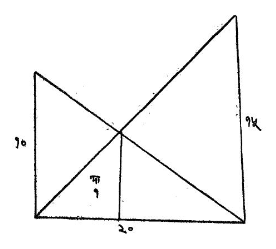
\includegraphics[scale=0.75]{graphics/Capture28.png}
\end{figure}
\vspace{-2mm}

 अत्र क्रियावतारार्थं वेण्वन्तरालभूमिमिष्टां विंशतिमितां प्रकल्प्य
सूत्रसम्पाताल्लम्बमानं यावत्तावत्प्रकल्प्य गणितमाकरे स्फुटम्~। अथ यावत्तावत्कल्पनां
विनापि लम्बज्ञानार्थमाह {\qt 'अथवा वंशसम्बन्धिन्यावाबाधे तद्युतिर्भूमिः'} इत्यादि~। अयमर्थः~। यथा यथा वंशो महाल्लँघुर्वा भवति तथा तथा तदाश्रिताबाधापि महती लघुर्वा भवति~। अतस्त्रैराशिकेनैवाबाधे ज्ञातुं शक्ये~। यथा यदि वंशयोगेन सकला भूर्लम्भ्यते तदैकेन
\newpage%%%%%%%%%%%%%%%%%%%%%%%%%%%%%%%%%%
\noindent वंशेन किमिति पृथगाबाधे १२~। ८~। अथ भूमि\textendash \,२०\textendash \,तुल्ये भुजे लघुवंशः १०
कोटिः तदा बृहदाबाधाभुजे १२ केति लब्धो लम्बः ६ यतो लघुवंशः कोटिर्भूमिर्भुजो
लघुवंशाग्रादितरवंशमूलगामि सूत्रं कर्ण इत्येतत्क्षेत्रवशादेव बृहदाबाधा भुजो
लम्बः कोटिरिति भवति~। एवं लघ्वाबाधा बृहद्वंशाभ्यामप्यनुपातो द्रष्टव्यः~। अथ
भूमिकल्पनं विनापि लम्बसिद्धिमाह {\qt 'अथवा वंशयोर्वघो योगहृतो यत्र तत्रापि वंशान्तरे लम्बः स्यादिति किं भूमिकल्पनयापि'} इति~। अत्रोपपत्तिः~। यदि वंशयोगेन
भूर्लभ्यते तदा बृहद्वंशेन किमिति लब्धा बृहद्वंशाश्रिताबाधा~। $\begin{matrix}
\vspace{-1mm}
\mbox{{भू ० वृ १}}\\
\vspace{-1mm}
\mbox{{वं ० यो १}}
\vspace{1mm}
\end{matrix}$~। अथ भूमितुल्ये भुजे लघुवंशः कोटिस्तदा बृहदाबाधया किमिति जातो लम्बः $\begin{matrix}
\vspace{-1mm}
\mbox{{व ० यो १ भू ० बृ ० ल १}}\\
\vspace{-1mm}
\mbox{{~~~~~~~~ व ० यो ० भू १}}
\vspace{1mm}
\end{matrix}$~। अत्र भाज्यभाजकयोः भूम्यापवर्ते जातं $\begin{matrix}
\vspace{-1mm}
\mbox{{बृ ० ल १}}\\
\vspace{-1mm}
\mbox{{वं ० यो १}}
\vspace{1mm}
\end{matrix}$~। एवमुपपन्नं वंशयोर्वधो योगहृतो लम्बः स्यादिति~॥~११४~॥
\vspace{2mm}

\begin{quote}
    {\qt देवज्ञवर्यगणसन्ततसेव्यपार्श्वबल्लालसञ्ज्ञगणकात्मजनिर्मितेऽस्मिन्~। \\
 बीजक्रियाविवृतिकल्पलतावतारेऽभूदेकवर्णजसमीकरणैकखण्डः~॥~७~॥}
\end{quote}

 \begin{center}
     इति श्रीसकलगणकसार्वभौमश्रीबल्लालदैवज्ञसुतकृष्णदैवज्ञविरचिते \\
 बीजविवृतिकल्पलतावतार एकवर्णसमीकरणखण्डविवरणम्~। \\
 अत्र ग्रन्थसङ्ख्या ४९०\\
\vspace{1.5cm}
\rule{0.2\linewidth}{0.5pt}
 \end{center}
 

\newpage
%%%%%%%%%%%%%%%%%%%%%%%%%%%%%%%%%%%%

\phantomsection \label{ch8}
\begin{center}
    {\LARGE \textbf{८ मध्यमाहरणम्}}\\
    \rule{0.2\linewidth}{0.9pt}
\end{center}

 तदेवं समशोधनादिना यथैकस्मिन् पक्ष एकजातीयम् अव्यक्तमेव परपक्षे च व्यक्तमेव
भवति तथापवर्तादिनोपायेन सम्पाद्य प्रश्नभङ्ग उक्तः~। अथ यद्यप्यपवर्तेनापि
तथा न भवति तत्र मध्यमाहरणलक्षणमुपायान्तरमिन्द्रवज्रयोपजातिकाभ्यां चाह\textendash 

\phantomsection \label{115}
\begin{quote}
    \ab 
     अव्यक्तवर्गादि यदावशेषं पक्षौ तदेष्टेन निहत्य किञ्चित्~। \\
 क्षेप्यं तयोर्येन पदप्रदः स्यादव्यक्तपक्षस्य पदेन भूयः~॥~\\
 व्यक्तस्य पक्षस्य समक्रियैवमव्यक्तमानं खलु लभ्यते तत्~। \\
 न निर्वहश्चेद्धनवर्गवर्गेष्वेवं तदा ज्ञेयमिदं स्वबुद्ध्या~॥~\\
 अव्यक्तमूलर्णगरूपतोऽल्पं व्यक्तस्य पक्षस्य पदं यदि स्यात्~। \\
 ऋणं धनं तच्च विधाय साध्यमव्यक्तमानं द्विविधं क्वचित्तत्~॥~११५~॥
\end{quote}

 एतानि सूत्राण्याचार्य एव व्याख्यातवान्~। अत्रोपपत्तिः~।
एकस्मिन् पक्षेऽव्यक्तम् एव परपक्षे च व्यक्तमेव यदि भवति तर्हि तयोः समत्वात्तस्याव्यक्तस्य
तद्व्यक्तं मानं भवतीति पूर्वमेवोक्तम्~। किन्तु व्यक्तशेषस्य
हरणार्थमव्यक्तशेषमपृथक्स्थमपेक्षितमतस्तादृशं यथा भवति तथा यतितव्यम्~। तत्र समयोः पक्षयोः समक्षेपे समशुद्धौ वा समगुणके वा समहरे वा मूलग्रहणे वा वर्गकरणे वा धनादिकरणे वा न 
समत्वहानिरिति तु स्पष्टम्~। अथ यत्राव्यक्तवर्गादिकं स्यादेकपक्षे
परपक्षे च रूपाण्येव 
तत्र मूलेन विना कदपि नाव्य-क्तस्यापृथक्स्थितिः~। अतः पक्षयोः
साम्याविरोधेन 
मूले ग्राह्ये~। तथा सति मूलयोरपि समत्वं स्यात्~। अत उक्तं \hyperref[115]{\textbf{पक्षौ तदेष्टेन निहत्य किञ्चित्क्षेप्यं तयोर्येन पदप्रदः स्यात्}} इति~। अत्रेष्टेन निहत्येत्युपलक्षणम्~। क्वचिदिष्टेन पक्षावपवर्तनीयौ क्वचिदिष्टं पक्षयोः शोध्यमित्याद्यपि ध्येयम्~। शेषोपपत्तिस्तु पूर्ववत्~। द्विविधमाने तु तत्रोदाहरणं \hyperref[124]{\textbf{वनान्तराले प्लवगाष्टभागः}} इति वक्ष्यमाणम्~। अत्र कपियूथं या १ अस्याष्टांशवर्गो द्वादशयुतो यूथसम इति समशोधने कृते जातौ पक्षौ $\begin{matrix}
\vspace{-1mm}
\mbox{{याव १ ~या ६ं४ रू ०}}\\
\vspace{-1mm}
\mbox{{याव ० या ० रू ७६८}}
\vspace{1mm}
\end{matrix}$~। अत्र पक्षयोर्द्वात्रिंश-
\thispagestyle{empty}
\afterpage{\fancyhead[CE] {बीजगणिते}}
\afterpage{\fancyhead[CO]{मध्यमाहरणम्}}
\cfoot{}
 \newpage
 %%%%%%%%%%%%%%%%%%%%%%%%%%%%%%%%%%

\noindent द्वर्गं १०२४ प्रक्षिप्य जातौ पक्षौ $\begin{matrix}
\vspace{-1mm}
\mbox{{याव १ या ६ं४ रू १०२४}}\\
\vspace{-1mm}
\mbox{{याव ० या ० ~रू ~२५६}}
\vspace{1mm}
\end{matrix}$~। अत्रोर्ध्वपक्षस्य पदमिदं $\begin{matrix}
\vspace{-1mm}
\mbox{{या १ रू ३ं२}}\\
\vspace{-1mm}
\mbox{{~~~~~~ १८}}
\vspace{1mm}
\end{matrix}$ इदं वा या १ं रू ३२~। द्वितीयपक्षस्य पदमिदं रू १६~। पदयोः सम-शोधनार्थं न्यासः $\begin{matrix}
\vspace{-1mm}
\mbox{{या १ रू ३ं२}}\\
\vspace{-1mm}
\mbox{{या ० रू १६}}
\vspace{1mm}
\end{matrix}$~। अयं वा $\begin{matrix}
\vspace{-1mm}
\mbox{{या १ं रू ३२}}\\
\vspace{-1mm}
\mbox{{या ० रू १६}}
\vspace{1mm}
\end{matrix}$~। अतो द्विविधमपि
मानम् उपपद्यते ४८~। १६~। नन्वव्यक्तपदरूपेभ्यो व्यक्तपदेऽधिके द्विविधं मानमनया युक्त्या
कथं न स्यात्~। शृणु तर्हि~। अव्यक्तपक्षजरूपाणामृणत्वे व्यक्तस्य धनत्वमेव~।
अस्मिन् प्रकारेऽव्यक्तशेषस्य धनत्वार्थमव्यक्तपक्षरूपाण्येव व्यक्तपक्षाच्छोध्यानि~। तानि च धनं भवतीति 
नास्त्यनुपपत्तिः~। अथ रूपाणां धनत्वे व्यक्तस्यर्णत्वमेवेति
द्वितीयप्रकारे व्यक्तमेव 
धनत्वार्थमितरपक्षाच्छोध्यम्~। व्यक्तरूपाणि त्वव्यक्तपक्षजपदरूपेभ्यः
शोध्यत्वादृणं 
भवति~। तानि यद्यधिकानि तदा ऋणं मानं स्यादिति द्वितीयं
सर्वथाप्यनुपपन्नम्~। 
अत उक्तं \hyperref[115]{\textbf{अव्यक्तमूलर्णगरूपतोऽल्पं व्यक्तस्य पक्षस्य पदं यदि स्यात्}} इति~। अथ 
यात्रालापे रूपोनमव्यक्तमस्ति तस्य वर्गे कर्तव्ये
रूपाणामृणत्वादव्यक्तस्यर्णत्वमुत्पद्यते~। तत्र पदग्रहणे रूपाणामेव ऋणत्वं नाव्यक्तस्य~। आलापे
रूपाणामृणत्वनिश्चयात्~। 
अव्यक्तस्यर्णत्वे कल्पिते ऋणं पक्षः स्यात्~। न ह्यधिकस्य शोध्यत्वे धनं
पक्षः 
सम्भवति~। भवतु वा क्वचिदस्य धनत्वम्~। तथाप्यालापसिद्धपक्षादन्यथात्वं तु
स्यादेव~। एवं सत्यालापसिद्धपक्षसमेन द्वितीयपक्षेण कथमस्य साम्यं स्यात्~। 
अतस्तत्समीकरणेनागतं मानमुपपन्नमेव स्यात्~। ऋणत्वात्~। न हि
व्यक्ते ऋणगते 
लोकस्य प्रतीतिरस्ति~। तस्मादेतादृश उदाहरणे व्यक्तपदे
व्यक्तमूलर्णगरूपतोऽल्पेऽपि 
द्विविधं मानं न सम्भवति~। रूपाणां धनत्वकल्पनेन सिद्धस्य
मानस्यानुपपन्नत्वात्~। 
एवमव्यक्तोनरूपवर्ग उद्दिष्टे सति तन्मूले व्यक्तस्यैव ऋणत्वं न रूपाणाम्~~। 
उक्तयुक्तेरविशेषात्~। अतस्तत्रापि द्विविधं मानं न सम्भवति~।
रूपाणामृणत्वकल्पनेन ~~सिध्दस्य ~~मानस्यानुपपन्नत्वात्~। ~इत्येवं ~~बहुधा ~~भवति~। ~क्वचित्क्षेपशोधनादिना 
शेषविधानां विपरीतमपि भवति~। क्वचिदव्यक्तस्य स्वतोऽप्यृणत्वे
द्विविधमूलसम्भवेऽपि 
द्वितीयमनुपपन्नं भवति~। अत एवाचार्यैर्द्विविधं
क्वचित्तदित्यनियमेनैवोक्तम्~। अथ 
द्वितीयमानस्यानुपपत्तौ वक्ष्यमाणमुदाहरणं प्रतीत्यर्थं प्रदर्श्यते~। 
\begin{quote}
\hyperref[125]{यूथात्पञ्चांशकस्त्र्यूनो वर्गितो गह्वरं गतः~। \\
 दृष्टः शाखामृगः शाखामारूढो वद ते कति~॥}
\end{quote}
\newpage
%%%%%%%%%%%%%%%%%%%%%%%%%%%%%%%%%%%%%%%%%%%%%%
\indent अत्र यूथं या ५ अस्य पञ्चांशः या १~। त्र्यूनः या १ रू ३ं~। वर्गितः याव १ या ६ं रू ९~। दृष्टेन युतो याव १ या ६ं रू १०~। यूथसम इति शोधने
कृते जातं 
\vspace{-2mm}

\begin{table}[h!]
    \centering\s
    \begin{tabular}{r}
     याव १ या १ं१ रू ०~।  \\
१० रू ०~। 
    \end{tabular}
\end{table}
\vspace{-2mm}

\noindent पक्षौ चतुर्भिः सङ्गुण्य तयोरेकादशवर्गं क्षिप्त्वा जातौ 
\vspace{-2mm}

\begin{table}[h!]
    \centering\s
    \begin{tabular}{r}
       याव ४ या ४ं४ रू १२१~। \\
 रू ८१~।
    \end{tabular}
\end{table}
\vspace{-2mm}

 अत्र रूपाणामेव ऋणत्वोद्देशादुक्तयुक्त्या पदमिदमेव या २ रू १ं१ नेदं
या २ं रू ११~। द्वितीयपक्षस्य पदं रू ९~। पुनः समीकरणेन लब्धं यावत्तावन्मानेन
१० उत्थापितो जातो राशिः ५०~। रूपाणां धनत्वे तु यावत्तावन्मानमिदं १~। 
राशिश्च ५ं~। नह्यस्य पञ्चांशः ५ त्रिभिरूनः सम्भवति~। एवमस्मिन्नेवोदाहरणे
यूथात्पञ्चांशकस्त्रिच्युत इति यथालापः स्यात्तदा द्वितीयमानमेव युक्तं न
तु 
पूर्वम्~। नहि पूर्वराशेः पञ्चांशः १० त्रिच्युतः सम्भवति~। अत एव\textendash
\begin{quote}
     {\qt द्युज्यकापमगुणार्कदोर्ज्यका स्वं युतिं खखखबाणसम्मिताम्~। \\
 वीक्ष्य भास्करमवेहि मध्यमं मध्यमाहरणमस्ति चेद्ध्रुवम्~॥~}
\end{quote}

 इत्यस्मिंस्त्रिप्रश्नोदाहरणे \,क्रान्तिज्यां \,यावत्तावन्मितां \,प्रकल्प्य \,ततोऽनुपातेन \,दोर्ज्यां चानीय तयोर्योगमुद्दिष्टयुतेर्विशोध्य तद्वर्गं
क्रान्तिज्यापवर्गोनत्रिज्यावर्गात्मकेन द्युज्यावर्गेण समं कृत्वा समशोधने कृते पक्षयोः पदग्रहणावसरे व्यक्तम् ऋणं रूपाणि धनम् इत्येव गृह्यते~। अत एव तदानयनसूत्रेऽपि तेनाढ्य ऊनो भवेदित्येवोक्तम्~। रूपाणामृणत्वे तु तेनाढ्य आढ्यो भवेदित्यप्युच्येत~। एवं मदुक्तयुक्त्या द्विविधमानोपपत्त्यनुपपत्ती सर्वत्रावधार्ये~। तदेवमुपपन्नं द्विविधं क्वचित्तदिति~। पदग्रहणार्थं \hyperref[115]{\textbf{पक्षौ तदेष्टेन निहत्य किञ्चित्~। क्षेप्यं तयोः}} इत्युक्तम्~॥~११५~॥\\

\vspace{-2mm}
 तत्र केन पक्षौ गुणनीयौ किं वा तयोः क्षेप्यमिति बालावबोधार्थं
श्रीधराचार्यकृतमुपायं दर्शयति\textendash

\phantomsection \label{116}
\begin{quote}
\ab
 'चतुराहतवर्गसमै रूपैः पक्षद्वयं गुणयेत्~। \\
 पूर्वाव्यक्तस्य कृतेः समं रूपाणि क्षिपेत्तयोरेव' इति~॥~११६~॥
\end{quote}

\newpage
%%%%%%%%%%%%%%%%%%%%%%%%%%%%%%%%%%

 अस्यार्थः~। चतुर्गुणितेनाव्यक्तवर्गाङ्केन पक्षद्वयं गुणयेत्~।
गुणनात् प्राग्यो व्यक्ताङ्कः तद्वर्गतुल्यानि रूपाणि पक्षयोः क्षिपेत्~। एवं
कृतेऽवश्यम् अव्यक्तपक्षस्य मूलं 
लभ्यते~। द्वितीयपक्षस्याप्येतत्समत्वान्मूलेन भाव्यम्~। एवं सति
व्यक्तपक्षस्य यदि 
मूलं न लभ्यते तदा तत्खिलमेवेत्यर्थात् सिद्धम्~। अत्र श्रीधराचार्यसूत्रे
मूलोपायस्याव्यक्तवर्गावुक्तसापेक्षतयोक्तत्वाद्यत्रैकस्मिन्पक्षेऽव्यक्तवर्णोऽव्यक्तं च
भवेत्तत्रैवास्य प्रवृत्तिरन्यत्र 
तु पदोपायः सुधिया स्वधिया चिन्त्यः~। अथ श्रीधराचार्यसूत्रोपपत्तिः~। यत्र
किल 
समशोधने कृत एकपक्षेऽव्यक्तवर्गोऽव्यक्तं चास्ति, इतरस्मिन्पक्षे
रूपाण्येव सन्ति तत्र 
प्रथमपक्षे रूपयोगेन विना कथमपि न मूललाभः~। यतः केवलाव्यक्तस्य वर्गकरणेऽव्यक्तवर्ग एव स्यात्~। रूपयुताव्यक्तस्य वर्गकरणेऽव्यक्तवर्गोऽव्यक्तं
रूपाणि च स्युः~। 
प्रकृते त्वव्यक्तवर्गोऽव्यक्तं च तिष्ठति स न कस्यापि वर्गः~। अतोऽवश्यं
रूपाणि 
क्षेप्याणि~। यद्यप्यव्यक्तशोधनेनाप्यव्यक्तमात्रस्य
शेषत्वादव्यक्तपक्षस्य मूलं लभ्यते 
तथापि द्वितीयपक्षे तथा सति साव्यक्तानि रूपाणि स्युरिति नास्य मूललाभ
इति 
पक्षयो रूपाण्येव क्षेप्याणि~। तत्र पदाव्यक्तवर्गस्य मूलं \,लभ्यते \,तदा \,केवलं \,रूपाण्येव \,क्षेप्याणि~। यदा \,त्वव्यक्तर्वगस्य \,मूलं \,न \,लभ्यते
तदाव्यक्तवर्गोऽपि तथा 
केनचिद्योज्यो गुणनीयो वा यथा मूलं लभ्येत~। तत्राव्यक्तवर्गयोगे
यद्यप्यव्यक्तपक्षस्य 
मूलं लभ्यते तथापि द्वितीयपक्षे साव्यक्तवर्गाणि रूपाणि
स्युरित्यव्यक्ताभावान्न 
मूललाभः~। न च पक्षयोरव्यक्तमपि क्षेप्यमिति वाच्यम्~। गौरवात्~। किं च 
यदव्यक्तपक्षेऽव्यक्तपक्षवर्गे द्वयमस्ति तदा पक्षयोः किं क्षेप्यम्~।
द्विसप्तचतुर्दशत्रयोविंशतिचतुस्त्रिंशत्सप्तचत्वारिंशद्द्विषष्ट्याद्यव्यक्तवर्गक्षेपे
प्रथमपक्षस्यैव मूलं लभ्येत नेतरस्य~। 
एकचतुराद्यव्यक्तवर्गक्षेपे तु प्रथमपक्षस्य मूलेन लभ्येत~। न च
यत्राव्यक्तवर्गद्वयमस्ति 
तत्र \,पक्षयोरेकस्याव्यक्तवर्गस्य \,शोधनेनोभयोरपि \,मूलं \,लभ्यत \,इति \,वाच्यम्~।
द्वितीय-पक्ष ऋणस्याव्यक्तवर्गस्य मूलाभावात्~। न च
त्रिपञ्चादिष्वव्यक्तवर्गेषु 
सत्स्वेकचतुरादयो व्यक्तवर्गाः पक्षयोः क्षेप्या
द्विषडादिष्वव्यक्तवर्गेषु सत्सु पक्षौ 
द्विषडादिभिर्गुणनीयाविति वाच्यम्~। अनुगमे सत्यननुगमस्यान्याय्यत्वात्~।
क्रियानिर्वाहस्यानियतत्वाच्च~। अतिगौरवाच्च~। यतोऽव्यक्तवर्गाव्यक्तरूपाणि तथा
क्षेप्याणि 
यथोभयपक्षयोरपि मूलं लभ्येत~। किं च मन्दबोधार्थं ह्युपायकथनम्~।
एतादृशस्य 
तु क्षेपस्य मन्ददुर्ज्ञेयतयोपायकथनं व्यर्थमेव स्यात्~। तदेवं
व्यक्तवर्गः केनचिद्गुणनीय 
एवेति सिद्धम्~। तत्र यदव्यक्तवर्गस्य मूलं लभ्यते तदा रूपाण्येव
क्षेप्याणि~। 
तानि कियन्तीति विचार्यते~। तत्र यद्यव्यक्तवर्गस्यैकमव्यक्तं मूलं लभ्यते
तर्ह्यव्यक्तार्धवर्गक्षेपेऽव्यक्तपक्षस्यावश्यं मूललाभः~। यतः \hyperref[31]{\textbf{कृतिभ्य आदाय पदानि}}
\newpage
%%%%%%%%%%%%%%%%%%%%%%%%%%%%%%%%%%%%%%%%
\noindent इत्यादिनाव्यक्तवर्गस्यैकमव्यक्तं मूलं रूपाणां त्वव्यक्तार्धतुल्यरूपाणि
द्वयोरभिहतिरव्यक्तार्धतुल्या स्यात्सा द्विनिघ्नी अव्यक्ततुल्या स्यादिति तच्छोधनेन
निःशेषता स्यात्~। 
एवं यत्राव्यक्तवर्गस्याव्यक्तद्वयं मूलं लभ्यते तत्राप्यनयैव युक्त्या
यथास्थिताव्यक्तचतुर्थांशवर्गतुल्यरूपक्षेपेऽवश्यं मूललाभः~। एवं यत्राव्यक्तत्रयं मूलं लभ्यते
तत्र 
पक्षस्थिताव्यक्तषडंशवर्गतुल्यरूपक्षेपेऽवश्यं मूललाभः~। तथा च
यत्राव्यक्तवर्गस्य 
मूलं लभ्यते तत्र तेन मूलाङ्केन द्विगुणेनाव्यक्ताङ्के भक्ते यल्लभ्यते
तद्वर्गतुल्यानि 
रूपाणि क्षेप्याणीति सिद्धम्~। \\

\vspace{-4mm}
 अथ यत्राव्यक्तवर्गाङ्कस्य न मूलं लभ्यते तत्र तेनेवाङ्केन गुणने
सत्यवश्यं 
मूललाभ इत्यव्यक्तवर्गाङ्केन पक्षौ गुणनीयौ~। \\

\vspace{-4mm}
 अथात्र पूर्वयुक्त्या रूपक्षेपः~। तदर्थमव्यक्तवर्गमूलाङ्केन
द्विगुणेनाव्यक्ताङ्को 
भाज्यः~। यत्राव्यक्तवर्गमूलाङ्कस्त्वगुणितोऽव्यक्तवर्गाङ्कः~। तथा
चागुणितेनाव्यक्तवर्गाङ्केन द्विगुणेनाव्यक्ताङ्को भाज्यः~।
पक्षगुणकेनागुणिताव्यक्तवर्गाङ्केन गुण्यश्च~। 
अत्र गुणहरयोरगुणिताव्यक्तवर्गाङ्केनापवर्ते कृते जातः
पूर्वाव्यक्ताङ्कस्य द्वयं 
भाजकः~। अतः पूर्वाव्यक्तार्धवर्गतुल्यानि रूपाणि क्षेप्याणीति
सिद्धम्~। एवं यत्र 
विनैव गुणनमव्यक्तवर्गाङ्कस्य मूलं लभ्यते तत्राप्ययुक्तयुक्त्या
पक्षावव्यक्तवर्गाङ्केन 
सङ्गुण्य पूर्वाव्यक्तार्धवर्गतुल्यानि रूपाणि प्रक्षिप्य च मूलं लभ्येतैव~। युक्तेरविशेषात्~। 
तदेवं पक्षावव्यक्तवर्गाङ्केन गुण्यौ पूर्वाव्यक्तार्धवर्गतुल्यानि रूपाणि
तयोः क्षेप्याणि 
चेति सिद्धम्~। एतावतैव पक्षयोर्मूललाभे सिद्धेऽप्यभिन्नत्वार्थं
पुनश्चतुर्भिर्गुणनमुक्तम्~। 
यतो वर्गेण वर्गगुणने कृते नास्ति वर्गत्वहानिः~। अथात्र पूर्वयुक्त्या
क्षेपः~।
अत्राव्यक्तवर्गे चतुर्भिर्गुणिते तन्मूलाङ्को द्विगुणितः स्यात्~। तेन च
द्विगुणेनाव्यक्ताङ्को
भाज्य इति जातः पूर्वाव्यक्तस्य पूर्वाव्यक्तवर्गाङ्कश्चतुर्गुणो भाजकः~।
पक्षगुणकोऽपि
तावानेवास्तीति गुणहरयोस्तुल्यत्वान्नाशे पूर्वाव्यक्ततुल्यानि रूपाणि
क्षेप्याणीति सिद्धम्~।
तदेवमुपपन्नम्\textendash
\begin{quote}
\hyperref[116]{चतुराहतवर्गसमै रूपैः पक्षद्वयं गुणयेत्~। \\
 पूर्वाव्यक्तस्य कृतेः समरूपाणि क्षिपेत्तयोरेव~॥} इति~। 
\end{quote}
 
 एवं कृतेऽपि यदि व्यक्तपक्षस्य मूलं न लभ्यते तदा करण्यात्मकं मूलं 
ग्राह्यम्~॥~११६~॥
\newpage
%%%%%%%%%%%%%%%%%%%%%%%%%%%%%%%%%%

 अथात्र शिष्यबुद्धिप्रसारार्थं विविधान्युदाहरणानि निरूपयन्नेकमुदाहरणं
मालिन्याह\textendash
\begin{quote}
    \eg 
    अलिकुलदलमूलं मालतीं यातमष्टौ \\
 निखिलनवमभागाश्चालिनी भृङ्गमेकम्~। \\
 निशि परिमललुब्धं पद्ममध्ये निरुद्धं \\
 प्रतिरणति रणन्तं ब्रूहि कान्तेऽलिसङ्ख्याम्~॥~११७~॥~
\end{quote}
 
 स्पष्टोऽर्थः~। अत्रालिकुलप्रमाणं द्विगुणवर्गात्मकं कल्प्यं यतोऽस्यैव
दलमूलं सम्भवति~। अतस्तथा कल्पितमाचार्यैः याव २~। गणितमाकरे स्फुटम्~। जातालिकुलसङ्ख्या ७२~॥~११७~॥ \\

\vspace{-2mm}
 अथान्यदुदाहरणं शार्दूलविक्रीडितेनाह\textendash
\begin{quote}
    \eg 
     पार्थः कर्णवधाय मार्गणगणं क्रुद्धो रणे सन्दधे \\
 तस्यार्धेन निवार्य तच्छरगणं मूलैश्चतुर्भिर्हयान्~। \\
 शल्यं षड्भिरथेषुभिस्त्रिभिरपि च्छत्रं ध्वजं कार्मुकं \\
 चिच्छेदास्य शिरः शरेण कति ते यानर्जुनः सन्दधे~॥~११८~॥~
\end{quote}

स्पष्टोऽर्थः~। अत्र कल्पितं बाणमानं याव १~। अस्यार्धं याव $\dfrac{\hbox{१}}{\hbox{२}}$~। चत्वारि
मूलानि या ४~। दृश्यबाणगणश्च रू १०~। एषामैक्यं याव $\dfrac{\hbox{१}}{\hbox{२}}$ या ८ रू २०~। राशिः याव १~।
समं कृत्वा पक्षौ समच्छेदीकृत्य च्छेदगमे शोधने च कृते पक्षयोः षोडश
रूपाणि 
प्रक्षिप्य मूले गृहीत्वा पुनः समीकरणेन लब्धं यावत्तावन्मानं १०~। जाता
बाणसङ्ख्या 
१००~॥~११८~॥ \\

\vspace{-2mm}
 अथान्यदुदाहरणमुपजातिकयाह\textendash
 \begin{quote}
     \eg 
      व्येकस्य गच्छस्य दलं किलादिरादेर्दलं तत्प्रचयः फलं च~। \\
 चयादिगच्छाभिहतिः स्वसप्तभागाधिका ब्रूहि चयादिगच्छान्~॥~११९~॥
 \end{quote}
\newpage
%%%%%%%%%%%%%%%%%%%%%%%%%%%%%%%%%%%%%%%%%%%%%%%%
 
 फलं चेति~। चस्त्वर्थो तथा सति फलशब्दस्योत्तरार्धेनान्वयः सुबोधः~। शेषं
स्पष्टम्~। अत्र गच्छमानं यावत्तावच्चतुष्टयरूपाधिकं या ४ रू १ प्रकल्प्य
गणितमाकरे स्फुटम्~। द्वितीयप्रकारेण फलसाधनार्थं पाटीस्थं सूत्रमिदम्\textendash
\begin{quote}
     {\qt 'व्येकपदघ्नचयो मुखयुक् स्यादन्त्यधनं मुखयुग्दलितं तत्~। \\
 मध्यधनं पदसङ्गुणितं तत्सर्वधनं गणितं च तदुक्तम्'} इति~॥~११९~॥ 
\end{quote}

अथान्यदुदाहरणमनुष्टुभाह\textendash
\begin{quote}
    \eg 
     कः खेन विहृतो राशिः कोट्या युक्तोऽथवोनितः~। \\
 वर्गितः स्वपदेनाढ्यः खगुणो नवतिर्भवेत्~॥~१२०~॥ 
\end{quote}
 
 स्पष्टोऽर्थः~। अत्र राशिः या १~। अयं खहृतः या $\begin{matrix}
\vspace{-1mm}
\mbox{{१}}\\
\vspace{-1mm}
\mbox{{०}}
\vspace{1mm}
\end{matrix}$~। अयं कोट्या युक्त 
ऊनितो वाविकृत एव~। खहरत्वात्~। अथायं या $\begin{matrix}
\vspace{-1mm}
\mbox{{१}}\\
\vspace{-1mm}
\mbox{{०}}
\vspace{1mm}
\end{matrix}$ वर्गितो याव $\begin{matrix}
\vspace{-1mm}
\mbox{{१}}\\
\vspace{-1mm}
\mbox{{०}}
\vspace{1mm}
\end{matrix}$~। स्वपदेन या $\begin{matrix}
\vspace{-1mm}
\mbox{{१}}\\
\vspace{-1mm}
\mbox{{०}}
\vspace{1mm}
\end{matrix}$ युक्तः याव १ या $\begin{matrix}
\vspace{-1mm}
\mbox{{१}}\\
\vspace{-1mm}
\mbox{{०}}
\vspace{1mm}
\end{matrix}$~। अयं खगुणो जातः याव १ या १~। गुणहरयोस्तुल्यत्वेन 
नाशात्~। अथामुं नवतिसमं कृत्वा समशोधने कृते पक्षौ चतुर्भिः सङ्गुण्य रूपं
प्रक्षिप्य प्राग्वज्जातो राशिः ९~॥~१२०~॥ \\

 \vspace{-2mm}
 अन्यदुदाहरणमनुष्टुभाह\textendash
\begin{quote}
    \eg 
     कः स्वार्धसहितो राशिः खगुणो वर्गितो युतः~। \\
 स्वपदाभ्यां खभक्तश्च जातः पञ्चदशोच्यताम्~॥~१२१~॥ 
\end{quote}
 
 स्पष्टोऽर्थः~। अत्र राशिः या १~। गणितमाकरे स्फुटम्~। मूलार्थे
रूपचतुष्टयं क्षेपः~॥~१२१~॥~\\

\vspace{-2mm}
अन्यदुदाहरणमार्ययाह\textendash
\begin{quote}
    \eg 
    राशिर्द्वादशनिघ्नो राशिघनाढ्यश्च कः समो यस्य~। \\
 राशिकृतिः षड्गुणिता पञ्चत्रिंशद्युता विद्वन्~॥~१२२~॥
\end{quote}
 \newpage
 %%%%%%%%%%%%%%%%%%%%%%%%%%%%%%%%%%%%%%%%
 स्पष्टोऽर्थः~। गणितमाकरे स्फुटम्~॥~१२२~॥\\ 

\vspace{-2mm}
 अथान्यदुदाहरणं सार्धानुष्टुभाह\textendash
\begin{quote}
    \eg 
    को राशिर्द्विशतीक्षुण्णो राशिवर्गयुतो हतः~। \\
 द्वाभ्यां तेनोनितो राशिवर्गवर्गोऽयुतं १०००० भवेत्~। \\
 रूपोनं वद तं राशिं वेत्सि बीजक्रियां यदि~॥~१२३~॥~
\end{quote}

 स्पष्टोऽर्थः~। रूपोनमयुतं भवेदिति योजनीयम्~। राशिः या १~।
अस्य 
यथोक्ते समशोधने कृते पक्षयोः याव ४ या ४०० रू १~।
एतावत्क्षिप्त्वा गणितमाकरे 
स्फुटम्~॥ १२३~॥ \\

\vspace{-2mm}
 अथ \hyperref[115]{\textbf{अव्यक्तमूलर्णगरूपतोऽल्पम्}} इत्यस्य सूत्रस्योदाहरणमुपजातिकयाह\textendash
 
\phantomsection \label{124}
\begin{quote}
    \eg 
    वनान्तराले प्लवगाष्टभागः संवर्गितो वल्गति जातरागः~। \\
 ब्रूत्कारनादप्रतिनादहृष्टा दृष्टा गिरौ द्वादश ते कियन्तः~॥~१२४~॥~
\end{quote}

 प्लवगा वानराः~। ब्रुदिति तन्नादानुकृतिः~। शेषं स्पष्टम्~। गणितमाकरे 
स्फुटम्~। द्विधा मानं चैतत् ४८~। १६~॥~१२४~॥ \\

\vspace{-2mm}
 अथ द्विधामानस्य क्वाचित्कत्वप्रदर्शनार्थमुदाहरणद्वयमनुष्टुब्द्वयेनाह\textendash
 
\phantomsection \label{125}
\begin{quote}
    \eg
    यूथात्पञ्चांशकस्त्र्यूनो वर्गितो गह्वरं गतः~। \\
 दृष्टः शाखामृगः शाखामारूढो वद ते कति~॥~\\
 कर्णस्य त्रिलवेनोना द्वादशाङ्गुलशङ्कुुभा~। \\
 चतुर्दशाङ्गुला जाता गणक ब्रूहि तां द्रुतम्~॥~१२५~॥~
\end{quote}
 
 त्रिभिरूनस्त्र्यूनः~। शाखामृगो वानरः~। स्पष्टमन्यत्~। गणितमाकरे स्पष्टम्~॥~१२५~॥\\

\vspace{-2mm}
अथान्यदुदाहरणमनुष्टुब्द्वयेनाह\textendash
\newpage
%%%%%%%%%%%%%%%%%%%%%%%%%%%%%%%%%%%%%%%%
 \begin{quote}
     \eg 
      चत्वारो राशयः के ते मूलदा ये द्विसंयुताः~। \\
 द्वयोर्द्वयोर्यथासन्नघाताश्चाष्टादशान्विताः~॥ \\
 मूलदाः सर्वमूलैक्यादेकादशयुतात्पदम्~। \\
 त्रयोदश सखे जातं बीजज्ञ वद तान्मम~॥~१२६~॥ 
 \end{quote}
 
 स्पष्टोऽर्थः~। अत्रोदाहरणे राशीनाम् अव्यक्तकल्पने क्रिया न निर्वहति~। अत
एकं मूलं यावत्तावत्प्रकल्प्य यथा सर्वमूलानि सिध्यन्ति तथा निरूपयति~।
तत्र राशिमूलकल्पनार्थम् आह\textendash \,{\qt 'अत्र राशी येन युतौ मूलदौ भवतः स किल राशिक्षेपः~। मूलयोरन्तरवर्गेण हतो राशिक्षेपो वधक्षेपो भवति~। तयो राश्योर्वधस्तेन युतोऽवश्यं मूलदः स्यादित्यर्थः'} इति~। \\

\vspace{-4mm}
 नन्वनेन ग्रन्थेन राशिमूलकल्पनं कथम् उक्तम्~। शृणु~। मूलयोरन्तरवर्गेण हतो
राशिक्षेपो वधक्षेपो भवतीत्यनेन राशिक्षेपस्य मूलान्तरवर्गस्य च वधो
वधक्षेपोऽस्तीति स्पष्टीकृतम्~। तथा च राशिक्षेपेण वधक्षेपे भक्ते यल्लभ्यते स एव 
मूलान्तरवर्गः~। अतः तस्य पदं मूलान्तरं स्यात्~। अतो यावत्तावदात्मकं 
प्रथममूलं तेन मूलान्तरेण युक्तं सत् द्वितीयमूलं स्यात्~। तदपि
पुनस्तेनैव युक्तं सत्तृतीयं स्यादित्यादि~॥~१२६~॥~ \\

\vspace{-2mm}
 इदमेवोक्तमाद्यपरिभाषायामपि\textendash

\phantomsection \label{127}
\begin{quote}
    \ab 
     राशिक्षेपाद्वधक्षेपो यद्गुणस्तत्पदोत्तरम्~। \\
 अव्यक्तराशयः कल्प्या वर्गिताः क्षेपवर्जिताः~॥~१२७~॥
\end{quote}
 
 अत्राव्यक्तराशयो राशिमूलान्येव~। अत एवैभ्यो राशिज्ञानमुक्तं
चतुर्थचरणेन \hyperref[127]{\textbf{वर्गिताः क्षेपवर्जिताः}} इत्यनेन~। यतो राशिः क्षेपेण योज्यस्तस्य मूलं
राशिमूलं भवत्यतो व्यस्त-विधिना राशिमूलं वर्गितं क्षेपोनं सद्राशिर्भवेदित्यर्थः~।
अथैतेभ्यो वधमूलान्याह\textendash 

\begin{quote}
    \qt
     'राशिमूलानां यथासन्नं द्वयोर्द्वयोर्वधाः~। \\
 राशिक्षेपोना राशिवधमूलानि भवन्ति~॥' इति~। 
\end{quote}
 
 स्पष्टोऽर्थः~। अत्रोभयोपपत्तिरुच्यते~। अत्र क्षेपयुतराशेर्मूले ज्ञाते
व्यस्तविधिना मूलवर्गे क्षेपोने राशिर्भवेदिति जातः प्रथममूलात्प्रथमराशिः प्रमूव १
क्षे १ं~।
 \newpage %%%%%%%%%%%%%%%%%%%%%%%%%%%%%%%%%%%%%%%%

एवं द्वितीयमूलाद्द्वितीयोऽपि द्विमूव १ क्षे १ं~। अनयोर्वधो येन
युक्तः सन्मूलदो भवेत् स एव वधक्षेपः~। तदर्थमनयोर्गुणनार्थं न्यासः 

\vspace{-2mm}
\begin{table}[h!]
    \centering\s
    \begin{tabular}{r}
      प्रमूव १~। द्विमूव १ क्षे १ं~। \\
क्षे १ं~। द्विमूव १ क्षे १ं~। 
\end{tabular}
\end{table}
\vspace{-2mm}

\noindent गुणनाज्जातं प्रमूव ० द्विमूव १ प्रमूव ० क्षे १ं द्विमूव ० क्षे १ं क्षेव १~। \\

\vspace{-4mm}
 अत्र द्वितीयखण्डे क्षेपगुणः प्रथममूलवर्ग ऋणमस्ति~। तृतीयखण्डे
क्षेपगुणो द्वितीयमूलवर्ग ऋणमस्ति~। अत्र लाघवान्मूलवर्गयोगः क्षेपगुण ऋणमिति
न्यासः 
\begin{center}
     प्रमूव ० द्विमूव १ मूवयो ० क्षे १ं क्षेव १ 
\end{center}

 अत्राद्यखण्डे मूलवर्गघातोऽस्ति~। य एव मूलवर्गघातः स एव मूलघातवर्ग 
इति तथा न्यासः 
\vspace{-4mm}

\begin{center}
     मूघाव १ मूवयो ० क्षे १ं क्षेव १~। 
\end{center}

 अत्र द्वितीयखण्डे मूलवर्गयोगः क्षेपगुणोऽस्ति~। तत्र मूलवर्गयोगस्य
खण्डद्वयम्~। 
एकं मूलान्तरवर्गः~। अपरं मूलयोर्द्विघ्नो घातः~। {\qt 'राश्योरन्तरवर्गेण द्विघ्ने घाते युते तयोः~। वर्गयोगो भवेत्'}~। इत्युक्तत्वात्~। अतो जाते वर्गयोगस्य खण्डे मूअंव १ मूघा २~। अनयोः क्षेपेण गुणने जातं द्वितीयखण्डं खण्डद्वयात्मकं मूअंव ० क्षे १ं मूघा ० क्षे २ं~। सर्वेषां खण्डानां क्रमेण न्यासः 
\vspace{-2mm}

\begin{center}
  मूघाव १ मूअंव ० क्षे १ं मूघा ० क्षे २ं क्षेव १~।  
\end{center}
 
 अयं हि राशिवधः~। अयं येन युतः सन्मूलदः स्यात्स एव वधक्षेपः~।
अत्र क्षेपगुणे मूलान्तरवर्गे क्षिप्ते शेषस्यास्य 
\vspace{-2mm}

\begin{center}
     मूधाव १ मूघा ० क्षे २ं क्षेव १~। 
\end{center}

\hyperref[31]{\textbf{कृतिभ्य आदाय पदानि}} इत्यादिना पदमिदमायाति~। मूघा १ क्षे १ं~। इदं हि वधमूलम्~। अत उपपन्नं मूलयोरन्तरवर्गेण हतो राशिक्षेपो वधक्षेपो
भवतीति~। राशिमूलानां यथासन्नं द्वयोर्द्वयोर्वधा राशिक्षेपोना वधमूलानि
भवन्तीत्यपि~। अनयैव युक्त्या द्वितीयतृतीययोस्तृतीयचतुर्थयोरपि
राश्योर्वधमूलोपपत्तिर्द्रष्टव्या~। 
एवमेकराशिमूलं यावत्तावत्प्रकल्प्य ततः सर्वमूलसिद्धिरुक्ता~। अथ प्रकृतोदाहरणे
\newpage
%%%%%%%%%%%%%%%%%%%%%%%%%%%%%%%%%%%%%%%%%%%%%%%%%
\noindent योजयति~। अत्रोदाहरणे राशिक्षेपाद्वधक्षेपो नवगुणो नवानां च मूलं
त्रयोऽतस्त्र्युत्तराणि राशिमूलानीत्यादिना~। शेषं स्पष्टम्~॥~१२७~॥ \\

\vspace{-2mm}
 अथान्यदुदाहरणमनुष्टुभाह\textendash
\begin{quote}
    \eg
     क्षेत्रे तिथिनखैस्तुल्ये दोःकोटी तत्र का श्रुतिः~। \\
 उपपत्तिश्च रूढस्य गणितस्यास्य कथ्यताम्~॥~१२८~॥~ 
\end{quote}

{\qt 'तत्कृत्योर्योगपदं कर्णः'} इति रूढस्य प्रसिद्धस्य गणितस्योपपत्तिः कथ्यताम्~। उपपत्तिमेव प्रष्टुमत्र श्रुतिप्रश्नो द्रष्टव्यः~। अत्र कर्णः या १~।
क्षेत्रदर्शनं
\begin{figure}[h!]
    \centering
    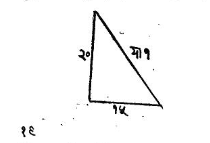
\includegraphics[scale=0.7]{graphics/Capture6.png}
\end{figure}

 अत्र कर्णस्य भूमित्वकल्पने दर्शनं 
\begin{figure}[h!]
    \centering
    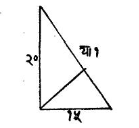
\includegraphics[scale=0.7]{graphics/Capture7.png}
\end{figure}

 क्षेत्रं परिवर्त्य दर्शनं 
\begin{figure}[h!]
    \centering
    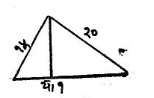
\includegraphics[scale=0.7]{graphics/Capture8.png}
\end{figure}

 अत्र लम्बादुभयतो ये त्र्यस्त्रे तयोरपि भुजकोटी पूर्वभुजकोट्यनुरूपे
भवतः~। तत्र भुजाश्रिताबाधा भुजो लम्बः कोटिः पूर्वभुजः कर्ण इत्येकं
त्र्यस्त्रम्~। लम्बो
\newpage
%%%%%%%%%%%%%%%%%%%%%%%%%%%%%%%%%%%%%%%%
\noindent भुजो द्वितीयाबाधा कोटिः पूर्वकोटिः २० कर्ण इत्यपरम्~। नन्वत्र
त्र्यस्रद्वयेऽपि 
लम्ब एव कथं न कोटिः~। सत्यम्~। दोःकोट्योर्नामभेदो न स्वरूपभेद इति 
यद्यप्यस्ति~तथापि प्रकृते भुजकोट्योः पूर्वभुजकोट्यनुरूपत्वविवक्षया न
तथा~। पूर्वं 
हि भुजात्कोटिर्महतीति प्रकृतेऽपि तथैव भाव्यम्~। किं च प्रकृतभुजकोट्योः
पूर्वभुजकोट्यनुरूपत्वे विवक्षिते सति भुजतुल्ये कर्णे यदि लम्बः
कोटिस्तदा कोटितुल्ये कर्णे 
केति त्रैराशिकेन कोटि-भेदेन भाव्यम्~। यद्वा
परस्परस्पर्धिदिशोर्भुजयोरेकतरस्य 
कोटिरिति सञ्ज्ञा स्वेच्छया क्रियताम्~। परं यावत्तावति कर्णे यदि
विंशतिमिता 
कोटिस्तदा विंशतिमिते कर्णे का कोटिरिति त्रैराशिकेन विंशतिमिते कर्णे परस्परस्पर्धिदिशोर्भुजयोर्मध्ये महान् एव भुज आबाधारूपः सिध्येन्न लम्बरूपो
लघुभुजः~। 
प्रमाणभुजस्य महत्त्वात्~। एवं यावत्तावति कर्णे यदि पञ्चदशमितो
भुजस्तर्हि 
पञ्चदशमिते कर्णे को भुज इति पञ्चदशमिते कर्णे
परस्परस्पर्धिदिशोर्भुजयोर्मध्ये 
लघुरेव भुज आबाधारूपः सिध्येन्न तु लम्बरूपो महान्भुजः~। प्रमाणभुजस्य
लघुत्वात्~। 
तदेवं यत्र कुत्रापि जात्ये त्र्यस्रे यदि यावत्तावत्कर्णो भूः कल्प्यते
तर्हि यावत्तावति 
कर्णे भुजो भुजस्तदा भुजतुल्ये कर्णे क इति त्रैराशिकेन या १~। भु १~। भु
१ भुजाश्रिताबाधा सिध्येत् $\begin{matrix}
\vspace{-1mm}
\mbox{{भुव १}}\\
\vspace{-1mm}
\mbox{{या १}}
\vspace{1mm}
\end{matrix}$~। एवं यावत्तावति कर्णे यदि कोटिः कोटिस्तदा
कोटितुल्ये कर्णे केति त्रैराशिकेन या १~। को १~। को १~। कोट्याश्रिताबाधा सिध्येत् $\begin{matrix}
\vspace{-1mm}
\mbox{{कोव १}}\\
\vspace{-1mm}
\mbox{{या १}}
\vspace{1mm}
\end{matrix}$~। आबाधयोर्योगोऽयं $\begin{matrix}
\vspace{-1mm}
\mbox{{भुव १ कोव १}}\\
\vspace{-1mm}
\mbox{{~~~~~ या १}}
\vspace{1mm}
\end{matrix}$~। अयं भूम्यनया या १ सम इति पक्षौ
समच्छेदीकृत्य 
च्छेदगमे जातौ $\begin{matrix}
\vspace{-1mm}
\mbox{{~~~~~ याव १}}\\
\vspace{-1mm}
\mbox{{भुव १ कोव १}}
\vspace{1mm}
\end{matrix}$~। अत्र पक्षयोः समत्वाद्य एव यावद्वर्गः स एव भुजकोटिवर्गयोग इति सिद्धम्~। प्रकृते कर्णो यावत्तावदात्मकोऽस्तीति
यावत्तावद्वर्गः कर्णवर्ग एव~। तस्मात्सिद्धं य एव कर्णवर्गः स एव भुजकोटिवर्गयोग इति~। अतोऽस्य पदं कर्णो भवितुमर्हति~। अत उपपन्नं तत्कृत्योर्योगपदं कर्ण इति~।
\newpage
%%%%%%%%%%%%%%%%%%%%%%%%%%%%%%%%%%%%%%%
\noindent अथवान्यथोपपत्तिः~। उद्दिष्टक्षेत्रमिदं 
\begin{figure}[h!]
    \centering
    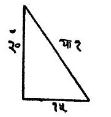
\includegraphics[scale=0.75]{graphics/Capture9.png}
\end{figure}

\noindent कर्णो यथा बहिर्भवति तथैतत्सममन्यत्क्षेत्रं योज्यते~। दर्शनं 
\begin{figure}[h!]
    \centering
    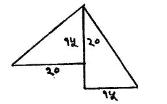
\includegraphics[scale=0.75]{graphics/Capture10.png}
\end{figure}

\noindent अथैवमेव तृतीयक्षेत्रं योज्यते 
\begin{figure}[h!]
    \centering
    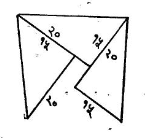
\includegraphics[scale=0.75]{graphics/Capture11.png}
   
\end{figure}

\noindent एव चतुर्थक्षेत्रयोगे दर्शनं 
\begin{figure}[h!]
    \centering
    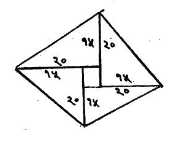
\includegraphics[scale=0.75]{graphics/Capture12.png}
\end{figure}
\newpage %%%%%%%%%%%%%%%%%%%%%%%%%%%%%%%%%%%%%%%%

 एवं \;समजात्यचतुष्टयेन \;तद्भुजकोट्यन्तरसमचतुर्भुजेन \;समकर्णेन \;पञ्चमेन \;चेति पञ्चभिः क्षेत्रैरेकं समकर्णं समचतुर्भुजं क्षेत्रं भवति~। \\

\vspace{-4mm}
 यत्तु समजात्यचतुष्टयमात्रेण समचतुर्भुजं भवति तद्विषमकर्णमेव दर्शनम्~।
\vspace{-2mm}
 
\begin{figure}[h!]
    \centering
    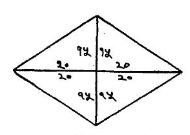
\includegraphics[scale=.8]{graphics/Capture13.png}
\end{figure}
\vspace{-2mm}

 अत्र द्विगुणो भुज एक कर्णो द्विगुणा कोटिरपरः~। यत्र तु भुजकोट्योः 
समत्वं तत्रान्तराभावात्प्रकारद्वयेनापि क्षेत्रचतुष्टयमात्रेण समकर्णं
भवति~। अथ प्रकृते समकर्णे विषमकर्णे च समचतुर्भुजे त्र्यस्रकर्णतुल्या एव भुजाः~।
परं समकर्णे चतुर्भुजे भुजकोट्यन्तरसमचतुर्भुजं क्षेत्रमधिकमस्ति~। अत एव 
भुजसमत्वेऽपि यथा यथा कर्णवैषम्यं भवति तथा तथा क्षेत्रसङ्कोचात्क्षेत्रफलमल्पं भवतीति प्रतिपादितमाचार्यैर्लीलावत्याम्~। \\

\vspace{-4mm}
 अथ प्रकृतमनुसरामः~। अत्र समकर्णे समचतुर्भुजे क्षेत्रे समश्रुतौ तुल्यचतुर्भुजे च {\qt 'तथायते तद्भुजकोटिघातः'} इत्यनेन भुजकोटिघातः फलं भवति 
अत्र भुजकोट्योः समतया भुजकोटिघातः समद्विघातो भवतीति भुजवर्ग एव 
क्षेत्रफलम्~। अतः क्षेत्रफले ज्ञाते सति तन्मूलं भुजमानं स्यात्~।
चतुर्भुजे यो 
भुजः स एव त्र्यस्रे कर्णोऽस्तीति कर्णोऽपि ज्ञातः स्यात्~। अतः
क्षेत्रफलं 
खण्डैः साध्यते~। तत्र त्र्यस्रे भुजकोटिघातार्धं फलं भवतीति
जातमेकस्मिंस्त्र्यस्रे 
क्षेत्रफलं भु ० को $\begin{matrix}
\vspace{-1mm}
\mbox{{१}}\\
\vspace{-1mm}
\mbox{{२}}
\vspace{1mm}
\end{matrix}$ इदं चतुर्गुणं सत् त्र्यस्रचतुष्टयस्य फलं स्यादिति
जातं भु ० को २~। अथ भुजकोट्यन्तरसमचतुर्भुजस्य समकर्णस्य क्षेत्रफलस्योक्तयुक्त्या
भुजकोट्यन्तरवर्गः फलं स्यात्~। तत्र भुजकोट्यन्तरमिदं भु १ं को १~। अस्य
वर्गः {\qt 'स्थाप्योऽन्त्यवर्गः'} इत्यादिना~। यद्वा खण्डगुणनेन जातः~। 
\vspace{-2mm}

\begin{center}
    भु १ भु ० को २ं कोव १~। 
\end{center}
\vspace{-2mm}
 
 इदमन्तर्लघुचतुर्भुजस्य क्षेत्रस्य फलं त्र्यस्रचतुष्टयफलेनानेन भु ० को २ युतं
\newpage
%%%%%%%%%%%%%%%%%%%%%%%%%%%%%%%%%%%%%%%%%%
\noindent सज्जातं प्रकृतचतुर्भुजस्य फलं भुव १ कोव १~। एवं भुजकोट्योर्द्विघ्नो
घातो भुजकोट्यन्तरवर्गेण युतः सन्भुजकोटिवर्गयोगो भवति~॥~१२८~॥~\\

\vspace{-2mm}
 एतदेवाहानुष्टुभा\textendash 
\begin{quote}
    \ab 
    दोःकोट्यन्तरवर्गेण द्विघ्नो घातः समन्वितः~। \\
 वर्गयोगसमः स स्याद्द्वयोरव्यक्तयोर्यथा~॥~१२९~॥
\end{quote}
 
 तत्र दोःकोटी उपलक्षणम्~। अत एव पाट्यामुक्तम्\textendash \,{\qt राश्योरन्तरवर्गेणे}त्यादि~। द्वयोरव्यक्तयोर्यथेति~। राशी या १ का १~। अनयोरन्तरवर्गः 
\vspace{-2mm}

\begin{center}
     याव १ याकाभा २ं  काव १~। 
\end{center}
\vspace{-2mm}

 अस्य द्विघ्नघातेनानेन याकाभा २ योगे जातो वर्गयोग एव याव १ काव १~। 
अथवा तान्येव क्षेत्रखण्डान्यन्यथा विन्यस्य क्षेत्रफलं साध्यते~। यथा\textendash\\

\vspace{-4mm}
 अत्र लघुचतुर्भुजस्य बाह्यभुजेन स्वमार्गवृद्धेन क्षेत्रं विच्छिद्य दर्शनं 
\begin{figure}[h!]
    \centering
    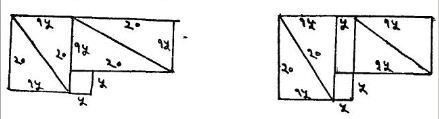
\includegraphics[scale=0.75]{graphics/Capture14.png}
\end{figure}

अतो मध्ये रेखामपनीय दर्शनम्~। 
\begin{figure}[h!]
    \centering
    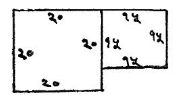
\includegraphics[scale=0.75]{graphics/Capture15.png}
\end{figure}

एवं जातं समचतुर्भुजद्वयम्~। एकं कोटितुल्यचतुर्भुजम् अपरं
भुजतुल्यचतुर्भुजम्~। द्वयमपि सकर्णम्~। अत उक्तवदेकत्र कोटिवर्गः क्षेत्रफलमपरत्र भुजवर्गः क्षेत्रफलमित्युभयोर्योगे जातो भुजकोटिवर्गयोगः प्रथमचतुर्भुजे क्षेत्रफलम्~। अस्य
पदं चतुर्भुजे भुजः स्यात्~। स एव त्र्यस्त्रे कर्ण इति वोपपन्नं {\qt 'तत्कृत्योर्योगपदं कर्णः'} इति~॥~१२९~॥
 \newpage 
 %%%%%%%%%%%%%%%%%%%%%%%%%%%%%%%%%%%%%%%%

 अथान्यदुदाहरणमनुष्टुभाह\textendash
\begin{quote}
    \eg 
     भुजात्त्र्यूनात्पदं व्येकं कोटिकर्णान्तरं सखे~। \\
 यत्र तत्र वद क्षेत्रे दोःकोटिश्रवणान्मम~॥~१३०~॥~

\end{quote}

 स्पष्टोऽर्थः~। अत्र कोटिकर्णान्तरमिष्टं कल्पितं २~। भुजात्त्र्यूनात्पदं
व्येकं सत्कोटिकर्णान्तरं भवत्यतो विलोमविधिना कोटिकर्णान्तरं २ सैकं ३ वर्गितं ९
त्रियुतं जातो 
भुजः १२~। अस्य वर्गः कोटिकर्णयोर्वगान्तरं १४४~। यतो भुजकोट्योर्वर्गयोगः
कर्णवर्गोऽस्त्यतः कर्णवर्गात्कोटिवर्गेऽपनीते भुजवर्ग एवावशिष्यते~। अतो
योऽयं भुजवर्गः 
१४४ तत्कोटिकर्णयोर्वर्गान्तरं कल्पितकोटिकर्णान्तमिदं २~। अतो वर्गान्तरं
राशिवियोगभक्तं योग इति जातः कोटिकर्णयोगः ७२~। {\qt 'योगान्तराभ्यां योगोऽन्तरेणोनयुतोर्द्धितः'} इति सङ्क्रमणसूत्रे जातौ कोटिकर्णौ ३५~। ३७ एवं
कोटिकर्णान्तरमेकं १ प्रकल्प्योक्तवज्जाता भुजकोटिकर्णाः ७~। २४~। २५~। एवमनेकधा~। अथ {\qt 'वर्गान्तरं राशिवियोगभक्तं योगः'} इत्यत्रोपपत्तिः~। वर्गान्तरं \,हि \,योगान्तरघातोऽस्ति~। अतोऽस्मिन्नन्तरेण \,भक्ते \,योगो \,लभ्येतैव \,योगेन \,वा भक्तेऽन्तरं लभ्येतेति
किं चित्रम्~। 
वर्गान्तरं योगान्तरघातोऽस्तीत्यत्र का युक्तिरिति चेत् शृणु समकर्णे~।
समचतुर्भुजे क्षेत्रे 
भुजवर्ग एव क्षेत्रफलं भवति~। अत उक्तविधक्षेत्रे भुजतुल्यो राशिः
क्षेत्रफलतुल्यस्तद्वर्गंश्च~। 
यथा राशी ७~। ५~। अनयोरुक्तवद्वर्गौ 

\begin{figure}[h!]
    \centering
    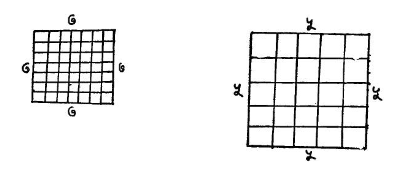
\includegraphics[scale=0.8]{graphics/Capture16.png}
\end{figure}
\newpage
%%%%%%%%%%%%%%%%%%%%%%%%%%%%%%%%%%%%%%%%%
\noindent सप्तवर्गात्पञ्चवर्गं विशोध्यम्~। इदं वर्गान्तरं 
\vspace{-2mm}

\begin{figure}[h!]
    \centering
    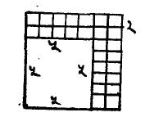
\includegraphics[scale=0.6]{graphics/Capture2.png}
\end{figure}
\vspace{-2mm}

\noindent अत्र पार्श्वद्वयेऽपि क्षेत्रशेषस्य विस्तारो भुजान्तरतुल्य एव स्यात्~।
भुजावेव राशी इति राश्यान्तरतुल्य एव विस्तारः स्यात् दैर्घ्यं त्वेकतरपार्श्वे
बृहद्भुजतुल्यमन्यस्मिन्पार्श्वे लघुभुजतुल्यं यथैवं 
\vspace{-2mm}

\begin{figure}[h!]
    \centering
    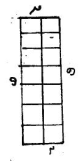
\includegraphics[scale=0.7]{graphics/Capture3.png}
\end{figure}
\vspace{-2mm}

\noindent एव वा 
\vspace{-2mm}

\begin{figure}[h!]
    \centering
    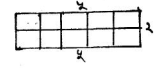
\includegraphics[scale=0.6]{graphics/Capture5.png}
\end{figure}
\vspace{-2mm}

\noindent अनर्योगे जातं क्षेत्रशेषमेव 

\begin{figure}[h!]
    \centering
    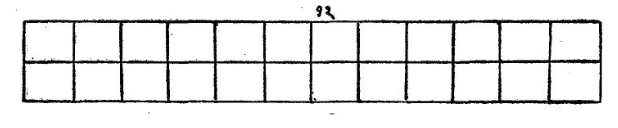
\includegraphics[scale=0.5]{graphics/Capture4.png}
\end{figure}
\newpage
% % % % % % % % % % % % % % % % % % % % % % % % % % % % % % % % % % % % %
\fancyhead[CE] {बीजगणिते}
\fancyhead[CO]{मध्यमाहरणम्}
\fancyhead[LE,RO]{\thepage}
\cfoot{}
\renewcommand{\thepage}{\devanagarinumeral{page}}
\setcounter{page}{176}
\s\onehalfspacing

 अस्य \,क्षेत्रस्य \,राशियोगतुल्यं \,दैर्घ्यं \,राश्यन्तरतुल्यो \,विस्तारश्चायते \,भुजकोटिघातः 
फलमिति योगान्तरघातस्य फलम्~। इदं क्षेत्रशेषं हि
पूर्वकल्पितराश्योर्वर्गान्तरं 
योगान्तरघातरूपमुपपन्नम्~॥~१३०~॥~\\

\vspace{-2mm}
 अथ वक्ष्यमाणोदाहरणोपयुक्तमन्यदनुष्टुब्द्वयेनाह\textendash

\phantomsection \label{131}
\begin{quote}
    \eg 
    वर्गयोगस्य यद्राश्योर्युतिवर्गस्य चान्तरम्~। \\
 द्विघ्नघातसमानं स्याद्द्वयोरव्यक्तयोर्यथा~॥~\\
 चतुर्गुणस्य घातस्य युतिवर्गस्य चान्तरम्~॥~\\
 राश्यन्तरकृतेस्तुल्यं द्वयोरव्यक्तयोर्यथा~॥~१३१~॥~
\end{quote}
 
 अत्र प्रथमसूत्रे वर्गयोगस्य युतिवर्गस्य चान्तरे कृतो द्विघ्नो घातो
भवतीति 
प्रतिपादितम्~। तत्र युक्तिर्द्वयोरव्यक्तयोर्यथेति~। यथा राशी या १ का १~। अनयोर्योगोऽयं याव १ काव १~। युतिवर्गोऽयं याव १ याकाभा २ काव १~।
वर्गयोगयुतिवर्गयोरन्तरमिदं याकाभा २~। राश्योर्द्विघ्नघातोऽस्ति~। पूर्ववत्क्षेत्रद्वारा
वा युक्तिः~। यथा 
राशी ३~। ५~। अनयोर्वर्गौ~। \\

\vspace{-4mm}
 युतिर्वर्गोऽयं 
\vspace{-4mm}

\begin{figure}[h!]
    \centering
    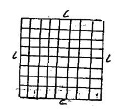
\includegraphics[scale=0.9]{graphics/Capture17.png}
\end{figure}

युतिवर्गाद्वर्गद्वयं विशोध्य शेषं
\newpage
%%%%%%%%%%%%%%%%%%%%%%%%%%
 अत्र क्षेत्रशेषखण्डयोरेकराशितुल्यो विस्तारः~। \\

\vspace{-4mm}
 परराशितुल्यं दैर्घ्यमिति प्रत्येकं राशिघातः फलम्~। अत उपपन्नं {\qt 'वर्गयोगयुतिवर्गयोरन्तरं द्विघ्नघातसमम्'} इति~। द्वितीयसूत्रे तु चतुर्गुणस्य
घातस्य युतिवर्गस्य चान्तरम्~। राश्यन्तरवर्गो भवति इति प्रतिपादितम्~। तत्र
युक्तिर्द्वयोरव्यक्तयोर्यथेति~। यथा राशी या १ का १~। अनयोर्घातश्चतुर्गुणोऽयं याकाभा ४ युतिवर्गश्चायं 
\vspace{-2mm}

\begin{center}
     याव १ याकाभा २ काव १~। 
\end{center}
\vspace{-2mm}

 युतिवर्गाच्चतुर्गुणघातेऽपनीते शेषमिदं 
\vspace{-2mm}

\begin{center}
    याव १ याकाभा २ काव १~। 
\end{center}
\vspace{-2mm}

इदं राश्यन्तरवर्ग एव~। यद्वा क्षेत्रगतोपपत्तिः सा तु मूल एव स्फुटास्ति~॥~१३१~॥~\\

\vspace{-2mm}
 अथोदाहरणमनुष्टुभाह\textendash
\begin{quote}
    \eg 
     चत्वारिंशद्युतिर्येषां दोःकोटिश्रवसां वद~। \\
 भुजकोटिवधो येषु शतं विंशतिसंयुतम्~॥~१३२~॥~
\end{quote}

अत्र किल भुजकोटिवधोऽयं १२०~। अयं द्विघ्नः सन् २४० भुजकोटियुतिवर्गस्य भुजकोटिवर्गयोगस्य चान्तरं स्यात्~। \hyperref[131]{\textbf{वर्गयोगस्य यद्राश्योर्युतिवर्गस्य चान्तरम्~। द्विघ्नघातसमानं स्यात्}} इत्युक्तत्वात्~। तत्र यो हि भुजकोटिवर्गयोगः स एव कर्णवर्गः~। अतो भुजकोटियुतिवर्गस्य कर्णवर्गस्य चान्तरमिदं २४०~। अत्र भुजकोटियुतिरेको राशिः~। कर्णोऽपरः~। अनयोर्वर्गान्तरमिदं २४०~। तत्र
योगान्तरघातसममित्युक्तत्वाद्भुजकोटियुतिकर्णयोगस्य
भुजकोटियुतिकर्णान्तरस्य च 
घातो भवति २४०~। तत्र भुजकोटियुतिकर्णयोगस्तु त्रयाणां योगो भवति~। स 
चात्र चत्वारिंशन्मित उद्दिष्ट एवास्ति ४०~। अतोऽनेन योगेन ४० योगान्तरघातेऽस्मिन् २४० भक्ते लब्धं भुजकोटियुतिकर्णान्तरं ६~। अथ
योगा-न्तराभ्यामेताभ्यां ४०~। ६ सङ्क्रमणेन जातौ राशी २३~। १७~। भुजकोटियुतिरेकः २३ कर्णोऽपरः १७~। 
अत्र लघुराशिरेव कर्णो ज्ञेयः~। भुजकोटियुतितस्तस्याधिक्यासम्भवात्~। 
उक्तमप्याचार्यैर्लीलावत्याम्~। 
\begin{quote}

    {\qt 'धृष्टोद्दिष्टमृजुभुजं क्षेत्रं यत्रैकबाहुतः स्वल्पा~। \\
 तदितरभुजयुतिरथवा तुल्या ज्ञेयं तदक्षेत्रम्~॥'} इति

\end{quote}
 \newpage
 %%%%%%%%%%%%%%%%%%%%%%%%%%%%%%%%%%%%
 अथ भुजकोटिवधे १२० चतुर्गुणे ४८० भुजकोटियुति\textendash \,२३\textendash \,वर्गादस्मात् ५२९ 
शोधिते शेषं ४९~। इदं भुजकोट्योरन्तरवर्गः~। \hyperref[131]{\textbf{चतुर्गुणस्य घातस्य युतिवर्गस्य चान्तरम्~। राश्यन्तरकृतेस्तुल्यम्}} इत्युक्तत्वात्~। अतोऽयं ४९ मूलं ७
भुजकोट्योरन्तरम्~। भुजकोटियोगश्चायं २३~। आभ्यां सङ्क्रमणेन जाते भुजकोटी 
८~। १५~॥~१३२~॥\\

\vspace{-2mm}
 अथान्यदुदाहरणमनुष्टुभाह\textendash
\begin{quote}
    \eg 
    योगो दोःकोटिकर्णानां षट्पञ्चाशत् ५६ वधस्तथा~। \\
 षट्शती सप्तभिः क्षुण्णो ४२०० येषां तान्मे पृथग्वद~॥~१३३~॥
\end{quote}
  
 स्पष्टोऽर्थः~। अत्र कर्णं यावत्तावन्मितं प्रकल्प्य गणितमाकरे स्फुटम्~॥~१३३~॥

\begin{quote}
{\qt दैवज्ञवर्यगणसन्ततसेव्यपार्श्वबल्लालसञ्ज्ञगणकात्मजनिर्मितेऽस्मिन्~। \\
बीजक्रियाविवृतिकल्पलतावतारेऽभूदेकवर्णजसमीकरणं सभेदम्~॥~}
\end{quote}

\begin{center}
     इति श्रीसकलगणकसार्वभौमश्रीबल्लालदैवज्ञसुतकृष्णगणकविरचिते \\
 बीजविवृतिकल्पलतावतारे निजभेदमध्यमाहरणसहितमेकवर्ण- \\
 समीकरणम्~॥~८~॥~\\
\rule{0.2\textwidth}{0.5pt}
\end{center}

 अत्र खण्डयोर्ग्रन्थसङ्ख्ये ४९०~। ३२५~। एवमेकवर्णसमीकरणे ग्रन्थसङ्ख्या~।
८१५~। एवमादितो जाता ग्रन्थसङ्ख्या ३३९५~।\\
\begin{center}
    \rule{0.2\textwidth}{0.5pt}
\end{center}
\newpage
%%%%%%%%%%%%%%%%%%%%%%%%%%%%%%%%%%%%%%%%%%%%%
\phantomsection \label{ch9}
\begin{center}
    {\LARGE \textbf{९ अनेकवर्णसमीकरणम्}}\\
\rule{0.2\textwidth}{0.5pt}
\end{center}

 एवमनेकवर्णानाम् एकवर्णपूर्वकत्वादादावेकवर्णसमीकरणमुक्त्वेदानीं क्रमप्राप्तमनेक-वर्णसमीकरणं शालिन्योपजातिकाद्वयेन शालिनीपूर्वार्धेन चाह\textendash
 
\phantomsection \label{134}
\begin{quote}
    \ab 
\hspace{-8mm} आद्यं वर्णं शोधयेदन्यपक्षादन्यान्रूपाण्यन्यतश्चाद्यभक्ते~। \\
\vspace{-7mm}

\hspace{-8mm} पक्षेऽन्यस्मिन्नाद्यवर्णोन्मितिः स्याद्वर्णस्यैकस्योन्मितीनां बहुत्वे~॥~\\
\vspace{-7mm}

\hspace{-8mm} समीकृतच्छेदगमे तु ताभ्यस्तदन्यवर्णोन्मितयः प्रसाध्याः~। \\
\vspace{-7mm}

\hspace{-8mm} अन्त्योन्मितौ कुट्टविधेर्गुणाप्ती ते भाज्यतद्भाजकवर्णमाने~॥~\\
\vspace{-7mm}

\hspace{-8mm} अन्येऽपि भाज्ये यदि सन्ति वर्णास्तन्मानमिष्टं परिकल्प्य साध्ये~। \\
\vspace{-7mm}

\hspace{-8mm} विलोमकोत्थापनतोऽन्यवर्णमानानि भिन्नं यदि मानमेवम्~। \\
\vspace{-7mm}

\hspace{-8mm} भूयः कार्यः कुट्टकोऽत्रान्त्यवर्णं तेनोत्थाप्योत्थापयेद्व्यस्तमाद्यात्~॥~१३४~॥
\end{quote}

 अस्मिञ्छालिनीपूर्वार्धेऽन्यत्पाठद्वयं दृश्यते~। 'भूयः कार्यः
कुट्टकादन्यवर्णाः' 
इति~। 'भूयः कार्यः कुट्टकादन्यवर्णस्तेनोत्थाप्योत्थापयेदन्तिमाद्यान्'
इति च~। एतानि 
सूत्राण्याचार्यैरेव सम्यग्व्याख्यातानीति नास्माभिर्व्याक्रियन्ते~।\\

 \vspace{-4mm}
 यथा शालिनीपूर्वार्धे व्याख्या~। यद्युत्थापने कृतेऽन्यवर्णमानं भिन्नं
लभ्यते तदात्र भूयः कुट्टकः कार्यः~। तेन
कुट्टकेनान्त्यवर्णमुत्थाप्याद्याद्व्यस्तमुत्थापयेत्~।
कुट्टको गुणविशेष इति प्रागेव निरूपितम्~। तेन कुट्टकेन सक्षेपेण
गुणेनान्त्ययोरन्त्येषु 
वा वर्णमानेषु यो वर्णस्तमुत्थाप्याद्याद्व्यस्तं पुनरुत्थापयेत्~।
यस्योन्मानस्य 
पूर्वमुत्थापने भिन्नं मानमभवत्तदुन्मानमाद्यम्~। तत आरभ्य पुनरपि
विलोमोत्थापनं 
कर्तव्यमित्यर्थः~। अयमेव पाठो मुख्यः~। आचार्यैः सूत्रविवरणावसरेऽस्यैव
विवरणात्~। 
तद्विवरणं यथा\textendash \,{\qt 'अथ यदि विलोमोत्थापने क्रियमाणे पूर्ववर्णोन्मितौ तन्मितिर्भिन्ना लभ्यते तदा कुट्टकविधिना यो गुणः सक्षेप उत्पद्यते स भाज्यवर्णस्य मानम्~। तेनान्त्यवर्णमानेषु तं वर्णमुत्थाप्य पूर्वोन्मितिषु
विलोमोत्थापनप्रकारेणान्यमानानि'} इति~। 'भूयः कार्यः कुट्टकादन्यवर्णः' इति पाठस्त्वसाधुः~। उत्थाप्येति पदस्या-
\thispagestyle{empty}
\afterpage{\fancyhead[CE] {बीजगणिते}}
\afterpage{\fancyhead[CO]{अनेकवर्णसमीकरणम्}}
\afterpage{\fancyhead[LE,RO]{\thepage}}
\cfoot{}
\newpage
%%%%%%%%%%%%%%%%%%%%%%%%%%%%%%%%%%%%%%%%%%%%%%%%5
% बीजगणितम् 
\noindent नन्वयात्~। अत्र यद्यप्याद्यमित्यध्याहृत्याद्यमुत्थाप्येति तदन्वयः
स्यात्तथाप्यन्त्यवर्णोत्थापनस्यानुक्तेर्न्यूनतादोषः स्यादेव~। अथ यदि
न्यूनतादोषपरिहारार्थमन्त्यवर्णमित्यध्याह्रियते तथा सति तेनान्त्यवर्णेनान्त्यवर्णम् उत्थाप्येति तदन्वयः स्यात्~। इह
हि यद्यन्यवर्णमानं 
भिन्नं स्यात्तदा भूयः कुट्टकादन्यवर्णः कार्य इत्युक्तेरन्यवर्णो
भाजकवर्ण एव~। एवं सति भाजकवर्णमानेनान्त्यवर्णमुत्थाप्येत्यर्थः पर्यवस्यति~। न चासौ युक्तः~। भाजकवर्णान्त्यवर्णयोर्भेदात्~। किं तु भाज्यवर्णस्यान्त्यवर्णस्य
चाभेदाद्भाज्यवर्णमानेनैवान्त्यवर्णोत्थापनं युक्तम्~। तदेवं द्वितीयपाठो न साधुः~। एवं तृतीयपाठोऽप्यसाधुः~।\\

\vspace{-2mm}
 अथैतस्यार्थस्य स्पष्टत्वार्थं वक्ष्यमाणमुदाहरणं लिख्यते~। 
\begin{quote}
\hyperref[139]{षड्भक्तः पञ्चाग्रः पञ्चविभक्तो भवेच्चतुष्काग्रः~। \\
 चतुरुद्धृतस्त्रिकाग्रो द्व्यग्रस्त्रिसमुद्धृतः कः स्यात्~॥} इति~। 
\end{quote}

 अत्र राशिः या १~। अयं \hyperref[139]{\textbf{षड्भक्तः पञ्चाग्रः}} इति लब्धिप्रमाणं कालकं प्रकल्प्य कालकगुणितो हरः स्वाग्रेण पञ्चकेन युक्तः का ६ रू ५~। यावत्तावत्सम इति साम्यकरणेन जाता यावत्तावदुन्मितिः 
\vspace{-2mm}

\begin{table}[h!]
    \centering\s
    \begin{tabular}{r}
         का ६ रू ५~। \\
        या १~। 
    \end{tabular}
\end{table}
\vspace{-2mm}

एवं पञ्चादिहरेषु नीलकादयो लभ्यन्त इति जाता यावत्तावदुन्मितयः 
\vspace{-2mm}

\begin{table}[h!]
    \centering\s
    \begin{tabular}{rp{5mm}rp{5mm}r}
     वी ५ रू ४~।&& पी ४ रू ३~।&& लो ३ रू २~। \\
 या~। &&या १~।&& या १~। 
    \end{tabular}
\end{table}
\vspace{-2mm}

आसां प्रथमद्वितीययोः समीकरणे लब्धा कालकोन्मितिः 
\vspace{-2mm}

\begin{table}[h!]
    \centering\s
    \begin{tabular}{r}
 नी ५ रू १ं~। \\
 का ६~। 
    \end{tabular}
\end{table}
\vspace{-2mm}

द्वितीयतृतीययोर्नीलकोन्मितिः 
\vspace{-2mm}

\begin{table}[h!]
    \centering\s
    \begin{tabular}{r}
 पी ४ रू १ं~। \\
 नी ५~।
    \end{tabular}
\end{table}
\newpage
%%%%%%%%%%%%%%%%%%%%%%%%%%%%%%%%%%%%%%%%%%%%%
एवं तृतीयचतुर्थ्योः पीतकोन्मितिः 
\vspace{-2mm}

\begin{table}[h!]
    \centering\s
    \begin{tabular}{r}
        लो ३ रू १ं \\
 पी ४~। 
    \end{tabular}
\end{table}
\vspace{-2mm}

\noindent इयमन्त्या~। \hyperref[134]{\textbf{अन्त्योन्मितौ कुट्टविधेर्गुणाप्ती}} इत्यादिना जाते लोहितपीतकयोर्माने सक्षेपे 
\vspace{-2mm}

\begin{table}[h!]
    \centering\s
    \begin{tabular}{l}
        ह ३ रू २ पी \\
 ह ४ रू ३ लो~। 
    \end{tabular}
\end{table}
\vspace{-2mm}

अथ नीलकोन्मानमिदं~ $\begin{matrix}
\vspace{-1mm}
\mbox{{पी ४ रू १ं}}\\
\vspace{-1mm}
\mbox{{~~~~ नी ५}}
\vspace{1mm}
\end{matrix}$~।\\

\vspace{-1mm}
\noindent अत्र नीलकपञ्चकस्य रूपोनपीतकचतुष्टयं मानम् अस्ति~। तत्र पीतकस्य कुट्टकसिद्धं मानमिदं ह ३ रू २~। अतो यद्येकस्य पीतकस्येदं मानं तदा पीतकचतुष्टयस्य किमिति पी १~। ह ३ रू २~। पी ४ त्रैराशिकेन जातं पीतकचतुष्टयस्य मानं ह १२ रू ८~।
इदं रूपोनं जातं नीलकपञ्चकस्य मानं ह १२ रू ७~। यदि नीलकपञ्चकस्येदं 
तदैकस्य नीलकस्य किमिति नी ५~। ह १२ रू ७ नी १~। त्रैराशिकेन नीलकस्य 
मानं भिन्नं लभ्यते 
\vspace{-2mm}

\begin{table}[h!]
    \centering\s
    \begin{tabular}{c}
        ह $\begin{matrix}
\vspace{-1mm}
\mbox{{१२}}\\
\vspace{-1mm}
\mbox{{५}}
\vspace{1mm}
\end{matrix}$ रू ७~।
    \end{tabular}
\end{table}
 \vspace{-2mm}

\noindent अतोऽत्र भूयः कुट्टकः कार्यः~। कुट्टको गुणकविशेषः~। स चोक्तविधिना जातः सक्षेपः श्वे ५ रू ४~। \hyperref[134]{\textbf{गुणाप्ती ते भाज्यतद्भाजकवर्णमाने}} इत्युक्तत्वादसौ कुट्टको
श्वे ५ रू ४ भाज्यवर्णस्य हरितकस्य मानं श्वे ५ रू ४ ह~। अनेनान्त्ययोः
पीतकलोहितकमानयोरनयोः $\begin{matrix}
\vspace{-1mm}
\mbox{{ह ३ रू २ पी}}\\
\vspace{-1mm}
\mbox{{ह ४ रु ३ लो}}
\vspace{1mm}
\end{matrix}$~। वर्णं हरितकमुत्थाप्याद्याद्व्यस्तं पुनरूत्थापयेत्~।
तदुत्थापनं यथा\textendash \,इह हरितकत्रयं रूपद्वययुतमेकस्य पीतकस्य मानमस्ति~। हरितकमानं च कुट्टकसिद्धमिदं श्वे ५ रू ४~। यद्येकस्य हरितकस्येदं मानं तर्हि हरितकत्रयस्य किमिति ह १~। 
श्वे ५ रू ४~। ह ३ त्रैराशिकेन जातं हरितकत्रयमानं श्वे १५ रु १२~। इदं रूपद्वययुतं जातं पीतकमानं श्वे १५ रू १४ पी~। अनयैव युक्त्या
लोहितकमानमपि
\newpage%%%%%%%%%%%%%%%%%%%%%%%%%%%%%%%%%%

\noindent श्वे २० रू १९ लो~। एवं जाते पीतकलोहितकयोर्माने $\begin{matrix}
\vspace{-1mm}
\mbox{{श्वे १५ रू १४ पी}}\\
\vspace{-1mm}
\mbox{{श्वे २० रू १९ लो}}
\vspace{1mm}
\end{matrix}$~। एवं जातं कुट्टकेनान्त्यवर्णोत्थापनम्~। \\

\vspace{-3mm}
 अथ लोहितपीतकयोराद्यान्नीलकादारभ्य व्यस्तम् उत्थापयेत्~। तत्र नीलकमानम् इदं $\begin{matrix}
\vspace{-1mm}
\mbox{{पी ४ रू १ं~।}}\\
\vspace{-1mm}
\mbox{{~~~~ नी ५~।}}
\vspace{1mm}
\end{matrix}$ इह रूपोनं पीतकचतुष्टयं नीलकपञ्चकस्य मानमस्ति~। तत्र
पीतकमानमिदं श्वे १५ रू १४ पी~। यद्येकस्य पीतकस्येदं तदा पीतकचतुष्टयस्य किमिति पी १~। श्वे १५ रू १४~। पी ४ त्रैराशिकेन पीतकचतुष्टयमानं श्वे ६० रू ५६~। इदं 
रूपोनं सज्जातं नीलकपञ्चकस्य मानं श्वे ६० रू ५५~। यदि नीलकपञ्चकस्येदं 
तदैकस्य किमिति नी ५~। श्वे ६० रू ५५~। नी १ त्रैराशिकेन 
जातं नीलकमानं श्वे १२ रू ११ नी~। अथ नीलकादाद्यः कालकस्तस्य 
मानमिदं $\begin{matrix}
\vspace{-1mm}
\mbox{{नी ५ रू १ं}}\\
\vspace{-1mm}
\mbox{{~~~~ का ६}}
\vspace{1mm}
\end{matrix}$~। इह रूपोनं नीलकपञ्चकं कालकषट्कस्य मानमस्ति~।
तत्र प्राग्वत्त्रैराशिकेन जातं नीलकपञ्चकमानं श्वे ६० रू ५५~। इदं रूपोनं सज्जातं
कालकषट्कमानं श्वे ६० रू ५४~। अतोऽनुपाताज्जातमेकस्य कालकस्य मानं श्वे १० रू ९ का~। अथ कालकादाद्यो यावत्तावत्तस्य मानमिदं $\begin{matrix}
\vspace{-1mm}
\mbox{{का ६ रू ५}}\\
\vspace{-1mm}
\mbox{{~~~~ या १}}
\vspace{1mm}
\end{matrix}$~। इह कालकषट्कं रूपपञ्चकयुतं यावत्तावतो मानमस्ति~। तत्र कालकषट्कस्यानुपातसिद्धं मानमिदं
श्वे ६० रू ५४~। इदं रूपपञ्चकयुतं जातं यावत्तावन्मानं श्वे ६० रू ५९ या~।
एवमन्यास्वपि यावत्तावदुन्मितिषूत्थापनेनेदमेव मानं  सिध्यति~। तदेवं जातानि
यावत्तावदादीनां मानानि व्यक्ताव्यक्तानि $\begin{matrix}
\vspace{-1mm}
\mbox{{श्वे ६० रू ५९ या}}\\
\vspace{-1mm}
\mbox{{श्वे १० रू\; ९ का}}\\
\vspace{-1mm}
\mbox{{श्वे १२ रू ११ नी}}\\
\vspace{-1mm}
\mbox{{श्वे १५ रू १४ पी}}\\
\vspace{-1mm}
\mbox{{श्वे २० रू १९ लो}}
\vspace{1mm}
\end{matrix}$~। अत्र श्वेतकस्य शून्ये माने कल्पिते जातो राशिः ५९~। कालकादयस्तु षडादिभाजकानां लब्धयः कल्पिता अतस्तन्मानानि जाताः क्रमाल्लब्धयः ९~। ११~। १~। १९~। एवं श्वेतकस्य मानं रूपमिष्टं 
प्रकल्प्य जातो राशिः ११९~। लब्धयश्च १९~। २३~। २९~। ३९~। एवमिष्टव-
\newpage
%%%%%%%%%%%%%%%%%%%%%%%%%%%%%%%%%%%%%%
\noindent शादानन्त्यम्~। अथोपपत्तिरुच्यते~। अत्र किल बहूनां मानान्यव्यक्तानि
सन्ति तत्र पूर्व-युक्त्यैकस्मिन्पक्षे यद्येकमेवाव्यक्तं स्यादन्यत्र च
रूपाण्येव स्युस्तदा तस्याव्यक्तस्य मानं सुबोधम्~। अतस्तथा यतितव्यं यथैकस्मिन् पक्ष एकमेवाव्यक्तं स्यात् समत्वाविरोधेन~। तत्र \hyperref[137]{\textbf{अश्वाः पञ्चगुणाङ्गमङ्गलमिताः}} इति वक्ष्यमाणम् उदाहरण् अधिकृत्य युक्तिरुच्यते~। अत्राश्वादीनां मूल्यान्यज्ञातानीति यावत्तावदादीनि कल्पितानि या १~। का १~। नी १~। पी १~। अतोऽनुपातेन निजनिजाश्वादीनां धनान्येकीकृत्य जातानि चतुर्णां समधनानि $\begin{matrix}
\vspace{-1mm}
\mbox{{या ५ का २ नी ८ पी ७}}\\
\vspace{-1mm}
\mbox{{या ३ का ७ नी २ पी १}}\\
\vspace{-1mm}
\mbox{{या ६ का ४ नी १ पी २}}\\
\vspace{-1mm}
\mbox{{या ८ का १ नी ३ पी १}}
\vspace{1mm}
\end{matrix}$~। अत्र चतुर्णामपि धनानि समानीति प्रथमद्वितीयधने अपि समे एव~। अत्रैकपक्षे
यथैकम् एवाव्यक्तं भवति तथा यतितव्यम्~। तत्रैकतरपक्ष एकं वर्णं विहाय यदवशिष्यते 
तत्तुल्यं चेदुभयोः पक्षयोः शोध्येत तर्ह्येकस्मिन्पक्ष एकम् एवा-व्यक्तं
स्यात्~। यं 
विहायावशिष्टं शोध्यते तस्मिन्पक्षे तस्यैव वर्णस्य शेषत्वात्~। तत्र कं
वर्णमपहाय 
शेषं पक्षयोः शोध्यमिति यद्यपि नास्ति नियमस्तथापि प्रथमातिक्रमे
कारणाभावात्प्रथमवर्णमपहाय शेषं पक्षयोः शोध्यम्~। अथ प्रकृते प्रथमवर्णमपहाय शेषमिदं
का २ नी ८ पी ७~। अस्मिन्पक्षयोः शोधिते जातमाद्यपक्षे या ५~।
द्वितीयपक्षे तु जातं या ३ का ५ नी ६ं पी ६ं~। अस्ति चानयोः समत्वम्~। समयोः
समक्षेपे 
समशुद्धौ वा समत्वाहानेः~। तथा सति यदेव यावत्तावत्पञ्चकस्य मानं तदेव 
नीलकषट्कपीतकषट्करहितस्य यावत्त्रयकालकपञ्चयोगस्यापीति सिद्धम्~। तथा च
यावत्पञ्चकस्य मानं ज्ञातुं यावात्त्रयस्यापि ज्ञानमपेक्षितम्~। तत्र यदि
स्वमानज्ञाने 
स्वमानज्ञानापेक्षा स्यात्तदात्माश्रयात्कल्पकोटिशतैरपि मानं ज्ञानं न
स्यात्~। अतः 
सा यथा न भवति तथा यतितव्यम्~। इतरपक्षे \,यः \,सजातीयो \,वर्णस्तत्तुल्यं \,पक्षयोः \,शोध्यम्~। प्रकृत \,इतरपक्षे \,सजातीयो वर्णोऽयं या ३~।
एतस्मिन्पक्षयोः 
शोधिते जातमाद्यपक्षे या २~। द्वितीयपक्षे का ५ नी ६ं पी ६ं~। एवं
कृते 
यदेव यावत्तावद्द्वयस्य मानं तदेव नीलकषट्कपीतकषट्करहितस्य कालकपञ्चकस्य 
मानमिति नास्ति स्वमानज्ञाने स्वमानज्ञानापेक्षा~। अत उक्तम् \hyperref[134]{\textbf{आद्यं वर्णं शोधयेदन्यपक्षादन्यान्रूपाण्यन्यतश्च}} इति~। \\

\vspace{-4mm}
 अथातस्त्रैराशिकम्~। यदि यावत्तावद्द्वयस्येदं मानं तदैकस्य यावत्तावतः
किमिति
 \newpage%%%%%%%%%%%%%%%%%%%%%%%%%%%%%%%%%%
\noindent या २~। का ५ नी ६ं पी ६ं~। या १ त्रैराशिकेन जातं
यावत्तावन्मानं $\begin{matrix}
\vspace{-1mm}
\mbox{{का ५ं नी ६ं पी ६}}\\
\vspace{-1mm}
\mbox{{या २}}
\vspace{1mm}
\end{matrix}$~। अत्र हरे याकारलिखनं
यावत्तावन्मानमिदमित्युपस्थित्यर्थं नतु 
यावत्तावद्द्वयं हरः~। प्रमा-णेच्छयोर्यावत्तावतापवर्तनात्~। अनपवर्ते
त्विच्छया गुणने क्रियमाणे भावितं स्यात्~। तदेवमुक्तप्रकारेण
प्रथमद्वितीययोर्द्वितीयतृतीययोस्तृतीयचतुर्थयोश्च धनयोः २ समशोधनेन जाताः प्रथमवर्णोन्मितयः 
\begin{table}[h!]
    \centering\s
    \begin{tabular}{rrr}
        का ५ नी ६ं पी ६ &का ३ नी १ पी १ं &का ३ नी २ं पी १~। \\
 वा २ &पी ३ &या २~ 
    \end{tabular}
\end{table}
\vspace{-2mm}

 तदेतदुक्तमाद्यभक्ते पक्षेऽन्यस्मिन्नाद्यवर्णोन्मितिः स्यादिति~। एवं
प्रथमतृतीययोः प्रथमचतुर्थयोर्द्वितीयचतुर्थयोश्च समशोधनेनान्या अपि
यावत्तावदुन्मितयः 
सम्भवन्ति~। परं प्रयोजनाभावान्न कृताः~। अथ भाज्यवर्णानां कालकादीनामिष्टानि मानानि प्रकल्प्यैक्यं कृत्वा यदि स्वहरेण ह्रियते तदा
भिन्नमभिन्नं वा 
प्रथमवर्णमानं स्यात्~। इतरेषां तु कल्पितान्येव~। तथा सति
मुखेनोद्दिष्टसिद्धिः~। 
अथ यद्यभिन्नमेव मानमपेक्षितं तर्हि यं कञ्चिदेकं वर्णं विहाय परेषां
मानानीष्टानि 
कल्प्यानि~। तथा सति भाज्य एको वर्णः कानिचिद्रूपाणि च स्युः~। अथ तस्य 
वर्णस्य मानं तथेष्टं कल्प्यं यथा तेनेष्टेन गुणितो वर्णाङ्कस्तै
रूपैर्युतो हरभक्तो निःशेषः स्यात्~। एवं कृते प्रथमवर्णमानमभिन्नमेव स्यात्~। \\

\vspace{-4mm}
 अथ तादृशस्येष्टस्य ज्ञानार्थमुपायः~। इह हि वर्णाङ्कः केन गुणितस्तै
रूपैर्युतः स्वहरहतो निःशेषः स्यादिति विचारः कुट्टके पर्यवस्यति~। अथ
कुट्टकविधिना यो गुण 
स्यात्तेन गुणितो वर्णाङ्कस्तै रूपैर्युतः स्वहरभक्तो निःशेषः स्यादेवेति
भाज्यवर्णस्य गुणतुल्ये माने कल्पिते भाजकवर्णस्य मानं लब्धितुल्यमभिन्नमेव स्यात्~। अत उक्तं \hyperref[134]{\textbf{कुट्टकविधेर्गुणाप्ती ते भाज्यतद्भाजकवर्णमाने~। अन्येऽपि भाज्ये यदि सन्ति 
वर्णास्तन्मानामिष्टं परिकल्प्य साध्ये}} इति~। अत्र भाज्यवर्णमानानां
यदिष्टकल्पनम् उक्तं तत्तेषां माने नियते सत्येव ज्ञेयम्~। यदि तु केनापि प्रकारेण
तन्मानं नियतं सिध्येत्तदा नियतेष्टकल्पनेन व्यभिचार एव स्यात्~।
यथास्मिन्नेवोदाहरणे यथा चतुर्णां समधनत्वमुद्दिष्टं तथा यदि 
\vspace{-1mm}

\begin{table}[h!]
    \centering\s
    \begin{tabular}{r}
      या ५ का २ नी ८ पी ७~। \\
 या ३ का ७ नी २ पी १~।
    \end{tabular}
\end{table}
 \newpage
 %%%%%%%%%%%%%%%%%%%%%%%%%%%%%%%%%%%%%%%%%
\noindent द्वयोरेवोद्दिष्टं स्यात्तदा तदुत्पन्नोन्मितौ $\begin{matrix}
\vspace{-1mm}
\mbox{{का ५ नी ६ं पी ६ं}}\\
\vspace{-1mm}
\mbox{{~~~~~~~~~~ या २}}
\vspace{1mm}
\end{matrix}$ भाज्यवर्णमानानामनियतत्वात् तदिष्टकल्पनेनोद्दिष्टसिद्धिः स्यात्~। यथात्र कालकादीनामिष्टानि कल्पितानि ४~। २~। १~। एभ्यो जातं यावत्तावन्मानं १~। जातान्यश्वादिमूल्यानि १~। ४~। २~। १~। यद्वा कल्पितानि ४~। १~। २~। जातं यावत्तावन्मानं १~। जातान्यश्वादिमूल्यानि १~। ४~। १~। २~। यद्वा कल्पितानि ६~। २~। १~। जातं यावत्तावन्मानं ६~। जातान्यश्वादिमूल्यानि ६~। ५~। २१~। यद्वा कल्पितानि ६~। १~। २ जातानि मूल्यानि ६~। ६~। २~। १~। यद्वा कल्पितानि~। ४~। १~। १~। जातानि 
मूल्यानि ४~। ४~। १~। १~। एवमिष्टवशादनेकधा~। यदि त्वनयोर्धनयोरन्यधनेनापि
समतोद्दिष्टा स्यात्तदा भाज्यवर्णमानानामिष्टकल्पने व्यभिचारः \,स्यादेव~।
नह्यन्यधनानुरोधेन \,काचित् \,क्रियात्र \,कृतास्ति \,येनान्यधनसमता सिध्येत्~। यदि तु
तदनुरोधिक्रियां 
विनापि तत्समता सिध्येत्तदा किमीदृग्धनं स्याद्यत्समं न स्यात्~।
तस्मादेतादृश्युदाहरणे 
भाज्यवर्णमानानामिष्टकल्पनं न युक्तम्~। किं तु नियतमेव तन्मानं साध्यम्~।
तच्च यथा 
समपक्षेभ्य आद्यवर्णमानं साधितं तथा भाज्याद्यवर्णस्यापि साध्यम्~। अत
उक्तं \hyperref[134]{\textbf{वर्णस्यैकस्योन्मितीनां बहुत्वे समीकृतच्छेदगमे तु ताभ्यस्तदन्यवर्णोन्मितयः प्रसाध्याः}} इति~। अत्र बहुत्वमनेकत्वम्~। उन्मितिद्वयादप्यन्यवर्णोन्मितिसम्भवात्~।
समीकृतच्छेदगम 
इत्यत्रोपपत्तिस्त्वेकवर्णसमीकरण आचार्येणैव स्पष्टीकृता~। अथ
प्रकृतदाहरणे यावत्तावदुन्मितयः $\begin{matrix}
\vspace{-1mm}
\mbox{{का ५ नी ६ं पी ६ं}}\\
\vspace{-1mm}
\mbox{{~~~~~~~~~ या २}}
\vspace{1mm}
\end{matrix}$~। $\begin{matrix}
\vspace{-1mm}
\mbox{{का ३ नी १ पी १ं}}\\
\vspace{-1mm}
\mbox{{~~~~~~~~~ या ३}}
\vspace{1mm}
\end{matrix}$~। $\begin{matrix}
\vspace{-1mm}
\mbox{{का ३ नी २ं पी १}}\\
\vspace{-1mm}
\mbox{{~~~~~~~~~ या २}}
\vspace{1mm}
\end{matrix}$~। अत्रहरे याकारस्यावास्तवत्वात् {\qt 'अन्योन्यहाराभिहतौ हरांशौ'} इत्यादिना भावितं न भवति~। 
याकारस्य वास्तवत्वेऽपि हराभ्यामपवर्तिताभ्यां यद्वा हरांशौ
गुण्यावित्युक्तत्वाद्वरयोर्यावत्तावतापवर्तनाद्भावितं न भवति~। अत्र
प्रथमद्वितीययोर्द्वितीयतृतीययोः प्रथमतृतीययोश्च जाताः कालकोन्मितयः $\begin{matrix}
\vspace{-1mm}
\mbox{{नी २० पी १६}}\\
\vspace{-1mm}
\mbox{{~~~~~ का ९}}
\vspace{1mm}
\end{matrix}$~। $\begin{matrix}
\vspace{-1mm}
\mbox{{नी ८ पी ५ं}}\\
\vspace{-1mm}
\mbox{{~~~~ का ३}}
\vspace{1mm}
\end{matrix}$~। $\begin{matrix}
\vspace{-1mm}
\mbox{{नी ४ पी ७}}\\
\vspace{-1mm}
\mbox{{~~~~ का २}}
\vspace{1mm}
\end{matrix}$~। अत्राप्येकतरस्येष्टं मानं प्रकल्प्य परस्य तथेष्टं कल्प्यं यथा कालकमानमभिन्नं भवेत्~। परं भाज्यवर्णमाननियतत्वे तदिष्टं न कल्पनमयुक्तम्~। भवति चात्र कालकोन्मितिभ्यां समीकृतच्छेदाभ्यां छेदगमादिना नीलकोन्मानं नियतं $\begin{matrix}
\vspace{-1mm}
\mbox{{पी ३१}}\\
\vspace{-1mm}
\mbox{{नी ४}}
\vspace{1mm}
\end{matrix}$~। अत्र यदेवैकत्रिंशत्पीतकमानं तदेवं नीलकचतुष्टयस्य~। अत्राप्यभिन्नत्वार्थं पीतकस्य तथेष्टं मानं
\newpage
%%%%%%%%%%%%%%%%%%%%%%%%%%%%%%%%%%
\noindent कल्प्यं यथा तद्गुणितः पीतकाङ्कश्चतुर्भिर्भक्तः शुध्येत्~। अस्ति चायं
कुट्टकविषयः~। अत्र भाज्यवर्णाङ्को भाज्यः~। भाजकवर्णाङ्को भाजकः~। यत्र तु भाज्ये
रूपाण्यपि स्युस्तत्र रूपाणि क्षेपः~। इह तु पीतकाङ्कः केन गुणितश्चतुर्भक्तः
शुध्येदित्येवास्तीति क्षेपाभावः~। \\
\vspace{-2mm}

 अथ कुट्टकार्थं न्यासः $\begin{matrix}
\vspace{-1mm}
\mbox{{भा ३१ क्षे ०}}\\
\vspace{-1mm}
\mbox{{हा ४ ~~~~}}
\vspace{1mm}
\end{matrix}$~। {\qt 'क्षेपाभावोऽथवा यत्र क्षेपः शुद्धो हरोद्धृतः~। ज्ञेयः शून्यं गुणस्तत्र क्षेपो हरहृतः फलम्'} इति जातौ लब्धिगुणौ $\begin{matrix}
\vspace{-1mm}
\mbox{{ल ०}}\\
\vspace{-1mm}
\mbox{{गु ०}}
\vspace{1mm}
\end{matrix}$~। अत्र \hyperref[59]{\textbf{इष्टाहतस्वस्वहरेण युक्ते ते वा भवेतां बहुधा गुणाप्ती}} इत्युक्तत्वादिष्टगुणा एकत्रिंशल्लब्धौ क्षेप्या इष्टगुणाश्चत्वारो गुणे क्षेप्याः~।
तत्रेष्टस्येच्छाधीनत्वेनानियतत्वाद्वर्णस्वरूपमिष्टं कल्पनीयम्~। वर्णस्य हि यद्यन्मानं कल्प्यते तत्तत्सम्भवतीति सर्वेष्टानामनुगमः 
स्यात्~। यदि तु व्यक्तम् इष्टं कल्प्यते तदा सर्वेष्टसिद्धिः~। अथ
प्रकृते यावत्तावदादीनां पीतकपर्यन्तानां मानानि नियतानि सन्तीति तेषामन्यतमस्येष्टकल्पने
सर्वेष्टानुगमो न स्यादत एभ्योऽन्यवर्ण इष्टः कल्पितः लो १~। अनेन गुणिते
स्वस्वहरे क्षिप्ते सति जातौ लब्धिगुणौ $\begin{matrix}
\vspace{-1mm}
\mbox{{लो ३१ रू ० ल}}\\
\vspace{-1mm}
\mbox{{लो ४ रू ० गु}}
\vspace{1mm}
\end{matrix}$~। अत्र पीतकाङ्को येन गुणितः
स्वस्वहरभक्तो निःशेषः स्यात्स गुण एव पीतकस्येष्टं मानं स्यात्~। यल्लभ्यते तदेव 
नीलकमानमभिन्नं स्यादिति गुणो भाज्यवर्णमानं लब्धिस्तु भाजकवर्णमानमिति~। तथा 
सति जाते नीलकपीतकयोर्माने $\begin{matrix}
\vspace{-1mm}
\mbox{{लो ३१ रू ० नी}}\\
\vspace{-1mm}
\mbox{{लो ४ रू ० पी}}
\vspace{1mm}
\end{matrix}$~। तदेवमन्त्योन्मितौ भाज्यवर्णमानं 
नियतं नास्तीति तस्य मानमिष्टं कल्प्यम्~। तत्रापि कुट्टकसिद्धगुणतुल्य
इष्टे कल्पिते भाजकवर्णमानमभिन्नं भवतीति गुणतुल्यं भाज्यवर्णमानं कल्प्यते~।
पूर्वोन्मितिषु तु 
भाज्यवर्णमानानां नियतत्वादिष्टकल्पनम् अयुक्तम्~। अत उक्तं \hyperref[134]{\textbf{अन्त्योन्मितौ कुट्टविधेः}} इत्यादि~। अथ पूर्वपूर्ववर्णोन्मितिषूत्तरोत्तरवर्णा भाज्यतया तिष्ठन्तीत्युत्तरोत्तरवर्णमानज्ञानं विना पूर्वपूर्ववर्णमानं न सिध्येदत उक्तं
\hyperref[134]{\textbf{विलोमकोत्थापनतोऽन्यवर्णमानानि}} इति~। अथ प्रकृते कालकोन्मितिरियं $\begin{matrix}
\vspace{-1mm}
\mbox{{नी २० पी १६}}\\
\vspace{-1mm}
\mbox{{~~~~~ का ९}}
\vspace{1mm}
\end{matrix}$~। अत्र विंशतिनीलकषोडशपीतकयोगो नवभक्तः कालकमानमस्ति~। तत्र यद्येकस्य नीलकस्येदं मानं तदा 
विंशतिनीलकानां किमिति नी १~। लो ३१ रू ०~। नी २० त्रैराशिकेन जातं 
नीलकविंशतेर्मानं लो ६२० रू ०~। अथैकस्य पीतकस्येदं तदा षोडशपीतकानां 
किमिति पी १~। लो ४ रू ०~। पी १६ त्रैराशिकेन जातं षोडशपीतकमानं लो ६४
\newpage
%%%%%%%%%%%%%%%%%%%%%%%%%%%%%%%%%%%%%%%%%%%%%%%%%%%

\noindent रू ०~। अनयोर्योगोऽयं लो ६८४ रू ०~। नवभक्तो जातं कालकमानं लो ७६ रू ० का~। एवमन्ययोरपि कालकोन्मित्योरिदमेव मानं सिध्यति~। अथवा यावत्तावदुन्मितिरियं $\begin{matrix}
\vspace{-1mm}
\mbox{{का ५ नी ६ं पी ६ं}}\\
\vspace{-1mm}
\mbox{{या २ ~~~~~~~~~}}
\vspace{1mm}
\end{matrix}$~। अत्रापि पूर्ववदनुपातेन जातानि
कालकपञ्चकादीनां 
मानानि लो ३८० रू ०~। लो १८ं६ रू०~। लो २ं४ रू ०~। एषां योगः लो १७० रू ०~। स्वहरेण द्विकेन भक्तो जातं यावत्तावन्मानं लो ८५ रू ० या~। एवमन्यास्वप्युन्मितिष्विदमेव मानं सिध्यति~। एवं सर्वत्र~। यस्य वर्णस्य
व्यक्तमव्यक्तं वा 
व्यक्ताव्यक्तं वा मानं सिध्यति तस्य वर्णस्यान्यत्र विद्यमानस्यापि
त्रैराशिकेनोत्थापनं द्रष्टव्यम्~। एतदेवोक्तमाचार्यैः सूत्रव्याख्यानान्ते {\qt 'इह यस्य वर्णस्य यन्मानमागतं व्यक्तमव्यक्तं व्यक्ताव्यक्तं वा तस्य मानस्याव्यक्ताङ्केन गुणने कृते तद्वर्णाक्षरस्य निरसनम् उत्थापनम् उच्यते'} इति~। अथ यदि विलोमोत्थापने क्रियमाणे मानं भिन्नमायाति तदा भिन्नत्वार्थं भूयः कुट्टकः कार्यः~। उक्तयुक्तेरविशेषात्~। तदेवं
सर्वमुपपन्नम्~। प्रकृते जातानि यावत्तावदादीनां मानानि $\begin{matrix}
\vspace{-1mm}
\mbox{{लो ८५ रू ० या}}\\
\vspace{-1mm}
\mbox{{लो ७६ रू ० का}}\\
\vspace{-1mm}
\mbox{{लो ३१ रू ० नी}}\\
\vspace{-1mm}
\mbox{{लो ~४ रू ० पी}}
\vspace{1mm}
\end{matrix}$~। अत्र सर्वेष्टानुगमार्थं लोहित  इष्टः कल्पितोऽस्ति~। तत्र यद्येकमिष्टं कल्प्यते तर्हि जातानि याव-त्तावदादिमानानि 
८५~। ७६~। ३१~। ४~। द्विकमिष्टं चेदेतानि १७०~। १५२~। ६२~। ८~। एवमिष्टवशादनेकधा~। एतान्येवाश्वादिमूल्यानि~॥~१३४~॥~\\

\vspace{-4mm}
 अथ शिष्यबुद्धिप्रसारार्थमुदाहरणानि निरूपयन्प्रथमं
तावदेकवर्णपठितमुदाहरणद्वयं निरूपयति~। पूर्व बीजाद्धि कल्पनागौरवेण तत्सिध्यति~। इह तु कल्पनालाघवेनेत्यस्ति विशेषः~। \\

\vspace{-2mm}
  तदुदाहरणद्वयञ्च\textendash
\begin{quote}
    \eg 
     माणिक्यामलनीलमौक्तिकमितिः पञ्चाष्ट सप्त क्रमात् \\
 एकस्यान्यतरस्य सप्त नव षट् तद्रत्नसङ्ख्या सखे~। \\
 रूपाणां नवतिर्द्विषष्टिरनयोस्तौ तुल्यवित्तौ तथा \\
 बीजक्ष प्रतिरत्नजानि सुमते मौल्यानि शीघ्रं वद~॥~१३५~॥
\end{quote}

 \newpage%%%%%%%%%%%%%%%%%%%%%%%%%%%%%%%%%%
\begin{quote}
    \eg 
     एको ब्रवीति मम देहि शतं धनेन \\
 त्वत्तो भवामि हि सखे द्विगुणस्ततोऽन्यः~। \\
 ब्रूते दशार्पयसि चेन्मम षड्गुणोऽहं \\
 त्वत्तस्तयोर्वद धने मम किं प्रमाणे~॥~१३६~॥~
\end{quote}

 माणिक्यामलनीलमौक्तिकमितिरित्येकम्~। एको ब्रवीतीत्यपरम्~। उदाहरणद्वयस्यापि गणितमाकर एव स्फुटम्~। \\

\vspace{-4mm}
 एको ब्रवीतीत्यादिसजातीयोदाहरणेष्यव्यक्तक्रियां सङ्क्षिप्य तत्परिपाकजेन
मार्गेण तदा-नयनमुक्तमस्मद्गुरुभिः श्रीविष्णुदैवज्ञैः~। तद्यथा\textendash

\begin{quote}
{\qt \textbf{स्वस्वैकयुक्तगुणदानजघातयोऽर्योऽनल्पः परः परगुणाभिहतस्तदैक्यम्~। \\
तत्स्यान्निरेकगुणघातहृतं हि राशिस्तत्सङ्गुणाधिकगुणः परवर्जितः सन्~॥\\
द्वितीयराशिमानं स्यादव्यक्तक्रियया विना~। \\
 व्यक्तमव्यक्तयुक्तं यद्ये न बुध्यन्ति ते जडाः~॥}} इति~।
\end{quote}
 
 अत्र परगुणाभिहत इत्यत्र परशब्दोऽन्यघातवाचको न तु पारिभाषिकः~। 
अन्य गुणकाभिहत इति वा पठनीयम्~। तत्सङ्गुणाधिकगुण इत्यत्राधिकोऽनल्पः पर 
इति यावत्~। तस्य गुणोऽधिकगुणो न त्वधिकश्चासौ गुणश्चेति कर्मधारय~।
तत्सङ्गुणः 
परगुण इति वा पठनीयम्~। शेषं स्पष्टम्~। अत्र प्रथमो गुणः २ दानं च १००~।
द्वितीयो गुणः ६ दानं च १०~। एकयुक्तेन गुणेन स्वस्वदाने गुणिते जातौ
स्वस्वैकयुक्तगुणदानजघातौ ३००~। ७०~। अत्रानल्पः परः ३००~। अयमन्यस्य गुणेन ६ गुणितः
१८००~। द्वितीयस्तु यथास्थित एव ७०~। अनयोरैक्यं १८७०~। इदं गुणघातेन 
१२ निरेकेण ११ हृतं जातो राशिः १७०~। अनेनाधिकस्य गुणो २ गुणितः ३४० 
परेणानेन ३०० वर्जितो जातो द्वितीयराशिरिति ४०~॥~१३५~॥~१३६~॥ \\

\vspace{-2mm}
 अथ शार्दूलविक्रीडितेनोदाहरणमाह\textendash

\phantomsection \label{137}
\begin{quote}
    \eg 
 अश्वाः पञ्चगुणाङ्गमङ्गलमिता येषां चतुर्णां धना- \\
 न्युष्ट्राश्च द्विमुनिश्रुतिक्षितिमिता अष्टद्विभूपावकाः~।\\
\newpage
%%%%%%%%%%%%%%%%%%%%%%%%%%%%%%%%%%%%%%%%%%%%%
 तेषामश्वतरा वृषा मुनिमहीनेत्रेन्दुसङ्ख्याः क्रमात् \\
 सर्वे तुल्यधनाश्च ते वद सपद्यश्वादिमौल्यानि मे~॥~१३७~॥
\end{quote}

 मङ्गलान्यष्टौ~। अश्वतरा वाम्यः~। महाराष्ट्रभाषया
वेसरशब्दवाच्याः~। शेषं 
स्पष्टम्~। गणितं तूपपत्तिविवरणावसरे स्पष्टीकृतम्~॥~१३७~॥\\

\vspace{-2mm}
 अथ वैचित्र्यार्थमाद्योदाहरणं प्रदर्शयति\textendash
\begin{quote}
    \eg 
     त्रिभिः पारावताः पञ्च पञ्चभिः सप्त सरसाः~। \\
 सप्तभिर्नव हंसाश्च नवभिर्बर्हिणस्त्रयः~। \\
 द्रम्मैरवाप्यते द्रम्मशतेन शतमानय~। \\
 एषां पारावतादीनां विनोदार्थं महीपतेः~॥~१३८~॥ 
\end{quote}

पूर्वश्लोकोक्तं पारावतसारसादिकं प्राणिजातं
त्रिपञ्चादिभिर्द्रम्मैरवाप्यते~। एवं 
सति द्रम्मशतेनैषां पारावतादीनां शतमानयेति व्याख्येयम्~। बर्हिणस्त्रय
इत्यत्र बर्हिणां त्रयमिति पाठश्चेत्साधुः~। यदा द्रम्मैरवाप्यत इति स्थाने
द्रम्मैवाप्यास्तदिति पाठश्चेत्साधुः~। शेषं स्पष्टम्~। अत्र प्रमाणे मौल्ययोगो जीवयोगश्च
चतुर्विंशतिरस्ति~। 
अपेक्षितश्च शतम्~। अतः किञ्चिद्गुणैः प्रमाणद्रव्यैर्जीवा ग्राह्याः~। तत्र तुल्यगुणकगुणितैः प्रमाणद्रव्यैर्जीवग्रहण उभयेषामपि योगः शतं न स्यात्~।
यतश्चतुर्गुणितानां 
प्रमाणद्रव्याणां योगः षण्णवतिस्तत्क्रीतजीवानामपि~। पञ्चगुणितानां तु
योगो विंशत्युत्तरशतं स्यात्~। यद्यपि चतुर्विंशतितुल्ये योगे यद्येको गुणस्तदा
शतमिते योगे 
क इति लब्धेन गुणकेन पञ्चविंशतिषडंशेन $\begin{matrix}
\vspace{-1mm}
\mbox{{२५}}\\
\vspace{-1mm}
\mbox{{६}}
\vspace{1mm}
\end{matrix}$ गुणने तद्योगः शतं स्यात्तथापि पारावतादयोऽखण्डा न लभ्येरन्~। तस्मादतुल्येन गुणकेन भाव्यम्~। कश्चिद्गुणः पारावतप्रमाणमौल्यस्य~। अपरः सारसमौल्यस्य~। 
अन्यो हंसमौल्यस्य~। इतरो मयूरमौल्यस्येति~। ते च गुणका न ज्ञायन्ते~। 
अतो यावत्तावदादयः कल्पिताः या १ का १ नी १ पी १~। एतैर्गुणितानि जातानि 
मूल्यानि या ३ का ५ नी ७ पी ९~। अथ द्रम्मत्रयेण मूल्येन यदि पञ्च पारावता
लभ्यन्ते तदा यावत्तावत्त्रयेण मूल्येन कियन्त इति ३~। ५~। या ३ त्रैराशिकेन
लब्धाः पारावता या ५~। एवं सारसादयोऽपि कालकपञ्चकादिमौल्यैर्लब्धः का ७ नी ६ पी
 \newpage%%%%%%%%%%%%%%%%%%%%%%%%%%%%%%%%%%
\noindent ३~। अथवा \,यद्गुणितानि \,द्रव्याणि \,स्युर्जीवा \,अपि \,तद्गुणिताः \,स्युरिति \,जातानि \,द्रव्याणि जीवाश्च $\begin{matrix}
\vspace{-1mm}
\mbox{{या ३ का ५ नी ७ पी ९}}\\
\vspace{-1mm}
\mbox{{या ५ का ७ नी ९ पी ३}}
\vspace{1mm}
\end{matrix}$~। अथ मौल्ययोगं जीवयोगं च पृथक्पृथक्शतसमं कृत्वा लब्धयावत्तावदुन्मानाभ्यां कालकोन्मानं विधाय शेषं गणितमाकरे 
स्फुटम्~। यद्वा केषां मौल्यानां योगः शतमस्तीति न ज्ञायते~। अतो
मौल्यान्येव यावत्तावदादीनि प्रकल्प्य या १ का १ नी १ पी १~। ततोऽनुपातेन
पारावतादीनानीय या $\begin{matrix}
\vspace{-1mm}
\mbox{{५}}\\
\vspace{-1mm}
\mbox{{३}}
\vspace{1mm}
\end{matrix}$ का $\begin{matrix}
\vspace{-1mm}
\mbox{{७}}\\
\vspace{-1mm}
\mbox{{५}}
\vspace{1mm}
\end{matrix}$ नी $\begin{matrix}
\vspace{-1mm}
\mbox{{९}}\\
\vspace{-1mm}
\mbox{{७}}
\vspace{1mm}
\end{matrix}$ पी $\begin{matrix}
\vspace{-1mm}
\mbox{{३}}\\
\vspace{-1mm}
\mbox{{९}}
\vspace{1mm}
\end{matrix}$~। पूर्वविधिनैव गणितं विधेयम्~। इयांस्तु विशेषः~। 
अत्र जीवानां योगः समच्छेदतया विधेयः~। शेषं पूर्ववत्~॥~१३८~॥\\

\vspace{-2mm}
 अथ \hyperref[134]{\textbf{'भूयः कार्यः कुट्टकः'}} इत्यस्योदाहरणमार्ययाह\textendash
 
\phantomsection \label{139}
\begin{quote}
    \eg 
      षड्भक्तः पञ्चाग्रः पञ्चविभक्तो भवेच्चतुष्काग्रः~। \\
 चतुरुद्धृतस्त्रिकाग्रो द्व्यग्रस्त्रिसमुद्धृतः कः स्यात्~॥~१३९~॥~
\end{quote}

 स्पष्टोऽर्थः~। अस्य गणितं सूत्रव्याख्यावसर एव स्पष्टीकृतम्~। आकरेऽपि स्पष्टम् अस्ति~। \\

\vspace{-4mm}
 अथ द्वितीयप्रकारेण कल्पितो राशिः या १~। अयं \hyperref[139]{\textbf{षड्भक्तः पञ्चाग्रः}} इति लब्धिं कालकं प्रकल्प्य तद्गुणितहरं का ६ स्वाग्रेण ५ युतं का ६ रू ५ राशिसमं 
कृत्वा लब्धं यावत्तावन्मानं का ६ रू ५~। अनेन राशिमुत्थाप्य जातो राशिः
का ६ रू ५~। एक आलापोऽस्य घटते~। पुनरयं 'पञ्चहृतश्चतुरग्रः' इति लब्धिं
नीलकं प्रकल्प्य तद्गुणितहरं नी ५ स्वाग्रेण ४ युतमस्य का ६ रू ५ समं कृत्वा
लब्धं कालकमानं भिन्नं $\begin{matrix}
\vspace{-1mm}
\mbox{{नी ५ रू १ं}}\\
\vspace{-1mm}
\mbox{{~~~~ का ६}}
\vspace{1mm}
\end{matrix}$~। कुट्टकेनाभिन्नं कालकमानं जातं पी ५ रू ४~। अथ
कालकषट्कं पञ्चयुतं पूर्वराशिरस्ति~। तत्रैकस्य कालकस्य मानमिदं पी ५ रू ४~। इदं षड्गुणितं जातं कालकषट्कस्य पी ३० रू २४~। इदं पञ्चयुतं जात उत्थापितः
पूर्वराशिः पी ३० रू २९~। अस्यालापद्वयं घटते~। एवमग्रेऽपि~। आकरेऽपि स्पष्टमिदम्~। एवमुत्थापनं सर्वत्र द्रष्टव्यम्~॥~१३९~॥
\newpage
%%%%%%%%%%%%%%%%%%%%%%%%%%%%%%%%%%%%%%%%%

अन्यदुदाहरणमार्ययाह\textendash
\begin{quote}
    \eg 
      स्युः पञ्चसप्तनवभिः क्षुण्णेषु हृतेषु केषु विंशत्या~।\\
 रूपोत्तराणि शेषाण्यवाप्तयश्चापि शेषसमाः~॥~१४०~॥~
\end{quote}

 स्पष्टोऽर्थः~। अत्र शेषाण्येतानि या १~। या १ रू १~। या १ रू २~। रूपोत्तराणि प्रकल्प्य कालकादीन् राशींश्च प्रकल्प्य गणितमाकरे स्पष्टम्~॥~१४०~॥~\\

\vspace{-2mm}
 अन्यदुदाहरणमनुष्टुभाह\textendash
\begin{quote}
    \eg 
      एकाग्रो द्विहृतः कः स्याद्द्विकाग्रस्त्रिसमुद्धृतः~।\\
 त्रिकाग्रः पञ्चभिर्भक्तस्तद्वदेव हि लब्धयः~॥~१४१~॥~
\end{quote}

 अत्र यावत्तावन्मितं राशिं प्रकल्प्य लब्धिर्द्विहृता सत्येकाग्रा
यथा भवति तथैतादृशी का २ रू १ प्रकल्प्य गणितमाकरे स्फुटम्~।\\

\vspace{-4mm}
 राशिर्द्विहृत एकाग्रः स्यात् तल्लब्धिरपि द्विहृतैकाग्रा स्यात्~।
एवम् अग्रेऽपि व्याख्ये-यम्~॥~१४१~॥~\\

\vspace{-2mm}
 अन्यदुदाहरणं शार्दूलविक्रीडितेनाह\textendash
 \begin{quote}
     \eg 
 कौ राशी वद पञ्चषट्कविहृतावेकद्विकाग्रौ ययोः\\
 द्व्यग्रं त्र्युद्धृतमन्तरं नवहृता पञ्चाग्रका स्याद्युतिः~।\\
 घातः सप्तहृतः षडग्र इति तौ षट्काष्टकाभ्यां विना\\
 विद्वन् कुट्टकवेदिकुञ्जरघटासङ्घट्टसिंहोऽसि चेत्~॥~१४२~॥
 \end{quote}

 स्पष्टोऽर्थः~। अत्र पञ्चहृतः सन्नेकाग्रो लघुराशिः षट्कमेव सम्भवति~।
एवं षट्कहृतो द्विकाग्रो लघुराशिरष्टावेव सम्भवति~। अतः कौ राशी
पञ्चषट्कविहृतावेकद्विकाग्रौ भवत इति प्रश्ने षट्काष्टकयोरेव
प्रथममुपस्थितिर्भवति~। यदृच्छया तयोः सर्वोऽप्यालापः सम्भवति~। तदत्र कल्पनां विनैव प्रश्नभङ्गः स्यादित्यत उक्तं षट्काष्टकाभ्यां विनेति~। अत्र राशी पञ्चषट्कविहृतौ \,यथैकद्विकाग्रौ \,भवतस्तथैतादृशौ \,या ५ रू १~। \,या ६ रू २ \,प्रकल्प्य घातालापकरणावसरे वर्गत्वान्महता क्रिया भवेदिति
पीतमेकेनोत्थाप्य प्रथमराशिं व्यक्तम् एव कृत्वा गणितमाकरे स्पष्टम्~॥~१४२~॥
\newpage%%%%%%%%%%%%%%%%%%%%%%%%%%%%%%%%%%२
 अन्यदुदाहरणमनुष्टुभाह\textendash
\begin{quote}
    \eg 
     नवभिः सप्तभिः क्षुण्णः को राशिस्त्रिंशता हृतः~।\\
 यदग्रैक्यं फलैकाढ्यं भवेत्षड्विंशतेर्मितम्~॥~१४३~॥~
\end{quote}

 राशिर्नवभिः सप्तभिः पृथग्गुणितः~। उभयत्रापि त्रिंशता हृतः~। शेषं
स्पष्टम्~। अत्र राशौ नवभिः सप्तभिः पृथग्गुणिते त्रिंशता भक्ते च लब्धिद्वयं
शेषद्वयं च पृथक्पृथक्स्यात्~। यदि तु गुणयोगेन राशिरेकनैव गुण्यते त्रिंशता च ह्रियते
तदा तत्र फलं फलैक्यं स्याच्छेषं च शेषैक्यं स्यात्~। यथा राशिः ५ नवभिः
सप्तभिः पृथग्गुणितः ४५~। ३५ त्रिंशता हृतः फले १~। १~। शेषे च १५~। ५~। अथ स एव राशिः ५ गुणयोगेन १६ गुणितः ८० त्रिंशता हृतः फलं २ शेषं च २०~। अत्र
हि फलं पूर्वफलैक्यमेव~। शेषं च पूर्वशेषैक्यमेव~। अत्रोदाहरणे
फलैक्यशेषक्ययोरेवावश्यकतया लाघवाद्गुणयोगं गुणं प्रकल्प्य गणितमाकरे स्पष्टम्~।
नन्वत्र
गुणयोगेन राशौ गुणिते हरेण भक्ते शेषैक्यमपि हरतष्टं स्यात्~। तत्र
यद्यपि
हरान्न्यूने शेषैक्ये सति तस्य यथास्थितस्य हरतष्टस्य चाविशेषान्न
काचित्क्षतिस्तथापि
हरादधिके शेषैक्ये तस्य यथास्थितस्य हरतष्टस्य च हरतुल्यमन्तरं स्यात्~।
फलैक्यं  च
सैकं स्यात्~। यथा राशिः ६ अयं नवभिः सप्तभिश्च पृथग्गुणितः ५४~। ४२
त्रिंशता हृतः फले १ं~। १ शेषे च २४~। १२~। अथ स एव राशिः ६ गुणयोगेन १६
गुणितः ९६ त्रिंशता हृतः फलं ३ शेषं च ६~। अत्र हि फलं पूर्वफलैक्यं सैकमस्ति~।
शेषं च सैकं हरतष्टमस्ति~। अतो गुणयोगे गुणे कल्पिते सति
फलैक्यशेषैक्ययोरन्यथात्वेन क्रियां व्यभिचरेदिति चेन्मैवम्~। गुणयोगे गुणे कल्पिते सति यदि
फलप्रमाणं कालकः  कल्प्येत तर्हि त्वदुक्तयुक्त्या
क्वचित्पूर्वफलैक्यशेषैक्ययोरन्यथात्वेन
क्रियां व्यभिचरेत्~। इह तु फलैक्यप्रमाणम् एव कालकः कल्प्यते~। तथा सति
हरगुणेऽस्मिन् भाज्यादपनीते शेषैक्यमपि यथास्थितं  स्यान्न हरतष्टमिति नास्ति फलैक्यशेषैक्ययोरन्यथात्वम्~। किं तु गुणयोगसम्बन्धिनोः फलशेषयोः
क्वचिदन्यथात्वं स्यात्~। परं तस्यानपेक्षितत्वादन्यथात्वेऽपि न काचित्क्षतिः~। अत एव
लब्धैक्यप्रमाणं कालक इत्येवोक्तमाचार्यैरपि~।\\

\vspace{-4mm}
 अथात्र प्रतीत्यर्थमस्मिन्नेवोदाहरणे 'यदग्रैक्यं फलैक्याढ्यमष्टत्रिंशन्मितं भवेत्'
इति प्रकल्प्य गणितं लिख्यते~। राशिः या १~। गुणयोगेन १६ गुणितः या १६~।
अयं त्रिंशद्भक्तः फलैक्यप्रमाणं कालकः का १~। अस्मिन् हरगुणे का ३०
भाज्यात् या
\newpage
%%%%%%%%%%%%%%%%%%%%%%%%%%%%%%%%%%%%%%%%%%%%%%

\noindent १६ अपनीते जातं शेषैक्यं या १६ का ३ं०~। इदं फलैक्येन कालकेन युतं या १६ का २ं९~। अष्टत्रिंशत्समं कृत्वा कुट्टकेन लब्धे यावत्तावत्कालकमाने $\begin{matrix}
\vspace{-1mm}
\mbox{{नी २९ रू ६ या}}\\
\vspace{-1mm}
\mbox{{नी १६ रू २ का}}
\vspace{1mm}
\end{matrix}$ अत्र फलैक्यशेषैक्ययोगस्येयत्तानिर्देशात्क्षेपोऽनुचित इति जाते
यावत्तावत्कालकमाने ६~। २~।
 तत्र यावत्तावन्मानं राशिः ६~। अयं नवभिः सप्तभिः पृथग्गुणितः
५४~। ४२~।
 त्रिंशद्भक्तः फले १~। १ शेषे च २४~। १२~। अत्र यदेव फलैक्यं तदेवं
कालकमानं
 न तु गुणयोगसम्बन्धि फलं शेषैक्येऽपि या १६ का ३ं०~। यावत्तावत्कालकौ
स्वस्वमानेनोत्थाप्य जातं शेषैक्यं यथास्थितमेव ३६ न तु हरतष्टम्~।
गुणयोगसम्बन्धि तु
 शेषमिदं ६ फलं च ३~। अथात्रैवोदाहरणे यदि फलप्रमाणं कालकः कल्प्यते
तदा
 पूर्ववज्जातं फलं का १ शेषं च या १६ का ३ं०~। इदं फलं फलैक्यं
सैकमस्तीति
 फलं रूपोनं सज्जातं फलैक्यं का १ रू १ं~। अथ शेषमपि शेषैक्यं
हरतष्टमस्तीति
 शेषं हरयुक्तं सज्जातं शेषैक्यं या १६ का ३ं० रू ३०~। अथ
फलैक्यशेषैक्ययोगं
 या १६ का २ं९ रू २९ अष्टत्रिंशत् समं कृत्वा कुट्टकेन
प्राग्वद्यावत्तावत्कालकमाने
 ६~। ३~। अत्र हि गुणयोगसम्बन्धि फलम् \,एव \,कालकः \,कल्पितोऽस्तीति \,कालकमानं \,तादृगेव \,सिद्धम्~। तदेवं \,कालकस्य फलत्वकल्पनेऽप्युदाहरणसिद्धिरस्ति~। इयांस्तु विशेषः~। फलप्रमाणे कालके कल्पिते यदि फलैक्यशेषैक्ययोरन्यथात्वं निश्चितं स्यात्तर्ह्येव फलं निरेकं शेषं च सहरं कर्तुं युज्यते नान्यथा~। फलैक्ये तु कालके कल्पिते न कोऽपि विचारोऽस्तीति लाघवात्फलैक्यमेव कालकः कल्प्यत इति सर्वमवदताम्~॥~१४३~॥~\\

\vspace{-2mm}
 अथान्यदुदाहरणमनुष्टुभाह\textendash
\begin{quote}
    \eg 
     कस्त्रिसप्तनवक्षुण्णो राशिस्त्रिंशद्विभाजितः~। \\
 यदग्रैक्यमपि त्रिंशद्धृतमेकादशाग्रकम्~॥~१४४~॥~

\end{quote}
   
 स्पष्टोऽर्थः~। अत्रापि गुणयोगो गुणः प्राग्वत् राशिः या १ गुणयोगेन १९
 गुणितः या १९~। त्रिंशतादृतो लब्धप्रमाणं कालकः का १~। अत्र यदग्रैक्यमपि
 त्रिंशद्धृतमिति शेषैक्यस्य हरतष्टस्यैवावश्यकतया फलप्रमाणमेव कालकः
कल्प्यते~।
 फलैक्यप्रमाणे कालके कल्पिते सति पूर्वोदाहरणोक्तयुक्त्या शेषैक्यं
यथास्थितमेव
 स्यान्न हरतष्टम्~। अत एवाचार्यैरत्र लब्धं कालक इत्येवोक्तम्~। अथ
लब्धिगुणं
 हरं भाज्यादपनीय जातमुक्तयुक्त्या त्रिंशत्तष्टं शेषैक्यं या १९ का ३ं०~।
तदेवं
\newpage
%%%%%%%%%%%%%%%%%%%%%%%%%%%%%%%%%%%%%%%%%%
\noindent यदग्रैक्यमपि त्रिंशद्धृतमिति द्वितीयालापस्य प्रथमालाप
एवान्तर्भूतत्वादिदमेवैकादशसमं 
कृत्वा प्राग्वज्जातो राशिः नी ३० रू २९~॥~१४४~॥~\\

\vspace{-2mm}
 अथान्यदुदाहरणमनुष्टुभाह\textendash
\begin{quote}
    \eg 
     कस्त्रयोविंशतिक्षुण्णः षष्ट्याशीत्याहृतः पृथक्~। \\
 यदग्रैक्यं शतं हृष्टं कुट्टकज्ञ वदाशु तम्~॥~१४५~॥~
\end{quote}
 
 स्पष्टोऽर्थः~। अत्र राशिः या १~। त्रयोविंशतिगुणितः या २३~। अमुं षष्ट्याशीत्या च पृथग्भक्त्वा कालकनीलकौ फले प्रकल्प्य यथास्वं लब्धिगुणं हरं
 भाज्यादपनीय जाते पृथक्शेषे या २३ का ६ं०~। या २३ ८ं०~। अनयोरैक्यं 
या ४६ का ६ं० नी ८ं०~। शतसमं कृत्वा लब्धा यावत्तावदुन्मितिः $\begin{matrix}
\vspace{-1mm}
\mbox{{का ६० नी ८० रू १००}}\\
\vspace{-1mm}
\mbox{{~~~~~~~~~~~~ या ४६}}
\vspace{1mm}
\end{matrix}$~। भाज्यभाजकौ द्वाभ्याम् अपवर्त्य जाता $\begin{matrix}
\vspace{-1mm}
\mbox{{का ३० नी ४० रू ५०}}\\
\vspace{-1mm}
\mbox{{~~~~~~~~~~~~ या २३}}
\vspace{1mm}
\end{matrix}$~। अत्र यावत्तावन्मानं भिन्नं 
लभ्यत इति कुट्टकेनाभिन्नं कार्यम्~। तत्र \hyperref[134]{\textbf{अन्येऽपि भाज्ये यदि सन्ति
वर्णास्तन्मानमिष्टं परिकल्प्य साध्ये}} इत्युक्तत्वात्कालकनीलकयोरन्यतरस्येष्टं
मानं कल्प्यम्~। परं तदिह न युक्तम्~। यतोऽत्र कालकनीलकावेकस्मादेव
भाज्यात्षष्ट्यशीत्योर्लब्धे~। तत्र
 षष्टिलब्धस्य कालकस्य व्यक्तकल्पने तदेव चरणोनमशीतिलब्धं बलात्स्यादिति
नीलकस्यापि व्यक्तमेव मानं स्यात्~। एवमशीतिलब्धस्य नीलकस्य व्यक्तत्वकल्पने
त्रैराशिकेन तदेव सत्र्यंशं बलात्षष्टिलब्धं स्यादिति कालकमानमपि व्यक्तमेव स्यात्~। तथा सति शेषयोगस्य नास्ति शतानुरोधिनी क्रियेति नोदाहरणसिद्धिः~। \\

\vspace{-4mm}
 अथ यद्यकतरवर्णस्येष्टं मानं प्रकल्प्य ततस्त्रैराशिकेन द्वितीयवर्णमानं
व्यक्तमकृत्वैव कुट्टकेन तन्मानं साध्येत तर्हि तदुक्तविधानादन्यथोत्पन्नमपि
बाधितमेव स्यात्~। न हि चरणोनात्षष्टिलब्धादन्यदशीतिलब्धं सम्भवति~।
सत्र्यंशादशीतिलब्धादन्यत्षष्टिलब्धं वा सम्भवति~॥~१४५~॥~\\

\vspace{-2mm}
 एतदेवानुष्टुभाह\textendash
\begin{quote}
    \ab 
     अत्राधिकस्य वर्णस्य भाज्यस्थस्येप्सिता मितिः~। \\
 भागलब्धस्य नो कल्प्या क्रिया व्यभिचरेत्तथा~॥~१४६~॥

\end{quote}
 
\newpage
%%%%%%%%%%%%%%%%%%%%%%%%%%%%%%%%%%%%%%%%%%
अस्यार्थः~। अत्र भाज्यस्थस्य भागलब्धस्याधिकवर्णस्य मितिरिष्टा न
कल्पनीया~। अधिकवर्णस्य कुट्टकोपयुक्तवर्णादतिरिक्तस्येत्यर्थः~। अथ
तदिष्टकल्पनेऽनिष्टमाह\textendash \,तथा सति क्रिया व्यभिचरेदिति~। अत्रोपपत्तिरुक्तैव~।
तदेवमुक्तविधकल्पनया नोदाहरणसिद्धिरस्तीत्यन्यथा यतितमाचार्यैः~। अत्र स्वस्वभागहारान्न्यूने शेषे यथा भवतो
 यथा च तद्योगः शतं स्यात्तथा शेषे प्रकल्प्य गणितमाकरे स्पष्टम्~। \\
\vspace{-4mm} 
 
ननु षष्ट्या यदि कालको लभ्यते तदशीत्या किमिति त्रैराशिकेनाशीतिं लब्धिमानीय 
का $\begin{matrix}
\vspace{-1mm}
\mbox{{३}}\\
\vspace{-1mm}
\mbox{{४}}
\vspace{1mm}
\end{matrix}$ प्राग्वच्छेषक्रियास्तु~। नह्येवं सति भाज्ये वर्णद्वयं भवति
येन द्वितीयवर्णेष्टकल्पनजो दोषः स्यादिति चेन्न, न ह्यत्र लब्ध्यनुपातो युक्तः~। अनुपातेन लब्धिसाधने
 हि यावतो भाज्यखण्डस्य षष्टिजा लब्धिरस्ति तावत एवाशीतिजा लब्धिः सावयवा
 स्यात्~। सा च न युक्ता~। न हि शेष उद्देश्ये सावयवा लब्धिः सम्भवति~।
यत्तु पूर्वमुक्तं कालकमानस्य \,व्यक्तकल्पने \,ततोऽनुपातेन \,नीलकमानमपि \,व्यक्तं \,स्यादिति \,तत्र \,व्यक्तत्वेनात्यल्पमन्तरं भवतीति न कोऽपि दोषः~। अथ यद्यनुपातजा
लब्धिः सावयवा
 न स्यात्तदा त्वदुक्तरीत्यापि भवेदेवोदाहरणसिद्धिः~। तथा हि~। राशिः या १~।
 अस्मात्त्रयोविंशतिगुणात्षष्ट्या लब्धिकल्पितं का १~।
अतोऽनुपातजाशीतिलब्धिः
 क ३~। अथ यथास्वं हरगुणां लब्धिं भाज्यादपनीय जाते शेषे $\begin{matrix}
\vspace{-1mm}
\mbox{{या २३ का २४ं०~।}}\\
\vspace{-1mm}
\mbox{{या २३ का १४०~।}}
\vspace{1mm}
\end{matrix}$ अत्र यावतो भाज्यखण्डात्षष्ट्या लब्धिस्तावत एवाशीत्या अपीति शेषे समे
एव भवतः~। अतः शेषयोगं शतसममथवा शेषं पञ्चाशत्समं कृत्वा कुट्टकेन लब्धे
यावत् कालकमाने नी २४० रू १९० या~। नी २३ रू १८ का~॥~१४६~॥\\

\vspace{-2mm}
 अथान्यदुदाहरणमनुष्टुभाह\textendash
\begin{quote}
    \eg 
   कः पञ्चगुणितो राशिस्त्रयोदशविभाजितः~। \\
 यल्लब्धं राशिना युक्तं त्रिंशञ्जातं वदाशु तम्~॥~१४७~॥~
\end{quote}
 
 स्पष्टोऽर्थः~। अत्राव्यक्ते राशौ कल्पिते तत्रोद्देशकालापे च कृत
उद्दिष्टगुणहरानुरोधिनी न काचित् क्रियास्तीति
नोदाहरणसिद्धिर्भवतीत्यत्राचार्यैरिष्टकर्मणैव राशिरानीतः ६५~॥~१४७~॥\\

\vspace{-2mm}
 अथ सार्धानुष्टुभोक्तमाद्योदाहरणं प्रदर्शयति\textendash 
 \newpage%%%%%%%%%%%%%%%%%%%%%%%%%%%%%%%%%%
\begin{quote}
    \eg 
     षडष्टशतकाः क्रीत्वा समार्घेन फलानि ये~। \\
 विक्रीय च पुनः शेषमेकैकं पञ्चभिः पणैः~॥~\\
 जाताः समपणास्तेषां कः क्रयो विक्रयश्च कः~॥~१४८~॥~
\end{quote}
 
 अस्यार्थः~। षट् अष्टौ शतं च धनं विद्यते येषां ते पडष्टशताः~। अर्शआदिभ्योऽजिति मत्वर्थीयोऽच्प्रत्ययः~। त एव षडष्टशतका इत्यत्र स्वार्थे
कन्प्रत्ययः~।
 धनं चात्र पणाः~। जाताः समपणा इत्युक्तेः~। तादृशा ये फलव्यापारिणः
समेनैव
 मूल्येन स्वस्वद्रव्यानुपातेन फलानि क्रीत्वा तानि समेनैव केनचिन्मूल्येन
विक्रीय च
 यच्छेषं पणविक्रयान्न्यूनं तद्यदृच्छया पान्थबाहुल्येन फलाल्पतया चैकैकं
फलं
 पञ्चभिः पञ्चभिः पणैर्विक्रीय च समपणाः समाः पणा येषां ते तथा जाताः~। 
एवं चेत्तर्हि तेषां फलव्यापारिणां क्रयः पणलभ्यफलप्रमाणं विक्रयः
पणदेयफलप्रमाणं
 किमिति प्रश्रः~। दलानीति पाठे ताम्बूलवल्लीपर्णानि कदल्यादिपर्णानि वा
ज्ञेयानि~। अथ 
तावदस्योदाहरणस्य गणितमाकरस्थं लिख्यते~। अत्र क्रयः या १~। विक्रय इष्टं
दशाधिकं
 शतं ११०~। क्रयः षड्गुणितो विक्रयेण हृतो लब्धं कालकः का १~। लब्धिगुणं
हरं षड्गुणिताद्राशेरपनीय शेषं या ६ का ११ं०~। इदं पञ्चगुणं लब्धियुतं \,जाताः \,प्रथमस्य \,पणाः \,या ३० का ५४ं९~। \,एवं \,द्वितीयतृतीययोरपि \,पणाः साध्याः~। तत्र
लब्धिरनुपातेन यदि षण्णां कालकस्तदष्टानां शतस्य च किमिति लब्धिरष्टानां का $\begin{matrix}
\vspace{-1mm}
\mbox{{४}}\\
\vspace{-1mm}
\mbox{{३}}
\vspace{1mm}
\end{matrix}$~। शतस्य च $\begin{matrix}
\vspace{-1mm}
\mbox{{का ५०}}\\
\vspace{-1mm}
\mbox{{~~ ३}}
\vspace{1mm}
\end{matrix}$~। लब्धिगुणं हरं भाज्यादपास्य ततः प्राग्वज्जाता द्वितीयस्य पणाः $\begin{matrix}
\vspace{-1mm}
\mbox{{या १२० का २१९६}}\\
\vspace{-1mm}
\mbox{{~~~~~~ ३}}
\vspace{1mm}
\end{matrix}$~। एवं तृतीयस्य पणाः $\begin{matrix}
\vspace{-1mm}
\mbox{{या १५०० का २७४ं५०}}\\
\vspace{-1mm}
\mbox{{~~~~~~~~~~~ ३}}
\vspace{1mm}
\end{matrix}$~। एते सर्वे
समा इति समच्छेदीकृत्य च्छेदगमे प्रथमद्वितीयपक्षयोर्द्वितीयतृतीययोः प्रथमतृतीययोश्च
समीकरणेन लब्धा यावत्तावदुन्मितिस्तुल्यैव $\begin{matrix}
\vspace{-1mm}
\mbox{{का ५४९}}\\
\vspace{-1mm}
\mbox{{या ३०}}
\vspace{1mm}
\end{matrix}$~। अत्र कुट्टकलब्धं
यावत्तावन्मानं $\begin{matrix}
\vspace{-1mm}
\mbox{{नी ५४९ रू ०}}\\
\vspace{-1mm}
\mbox{{२२~}}
\vspace{1mm}
\end{matrix}$~। नीलकमेकेनोत्थाप्य जातः क्रयः ५४९ इति~। \\

\vspace{-2mm}
 अथात्र किञ्चिद्विचार्यते~। इह हि षड्गुणितात्क्रयाद्विक्रयहृताद्यदि
कालको
 लभ्यते तदष्टगुणिताच्छतगुणिताच्च किमिति त्रैराशिकेन
लब्धिसाधनं कृतमाचार्यैः~।
 तत्र पृच्छ्यते~। षड्गुणितस्य क्रयस्य येह लब्धिः कल्पिता सा किमशेषा
सशेषा\\
\newpage
%%%%%%%%%%%%%%%%%%%%%%%%%%%%%%%%%%%%%%%%%%%%%%%%%%%%%%%%%%%%%
\noindent वा~। आद्ये शेषाभावाच्छेषमेकैकं पञ्चभिः पणैरित्यालापविरोधः~। द्वितीये
तु तादृशलब्धेरनुपातेन गुणान्तरलब्धिं तु साधनमयुक्तम्~। गुणान्तरलब्धौ हि
शेषोत्थलब्धितुल्यमन्तरं स्यात् इति व्यभिचारः स्यात्~। तद्यथा\textendash \,भाज्यभाजकौ $\begin{matrix}
\vspace{-1mm}
\mbox{{१५}}\\
\vspace{-1mm}
\mbox{{१३}}
\vspace{1mm}
\end{matrix}$~। अत्र षड्गुणितभाज्यात् ९० लब्धिरियं ६ शेषमिदं १२~। अथ षड्गुणितभाज्याच्चेदियं लब्धिः ६ तदष्टगुणिताच्छतगुणि-ताच्च केति त्रैराशिकेन जाते अष्टगुणितशतगुणितभाज्ययोः क्रमेण लब्धी ८~। १००~।
 न चैते युक्ते~। यतोऽष्टगुणितभाज्यादस्मात् १२० शतगुणितभाज्यादस्माच्च
१५००
 क्रमेण लब्धी ९~। ११५~। अतो लब्ध्यनुपातो न युक्तः~। ननु केवलभाज्ये
हरभक्ते यच्छेषं
 तद्गुणितगुणकादधिके हरे शेषोत्था लब्धिर्नैव सम्भवति~। तथा सति व्यभिचारः
कर्तव्यः~। तथाहि~। केवलभाज्यस्य हि खण्डद्वयम् अस्ति~। यावद्धरभक्तं तावदेकम्~।
शेषतुल्यम् अपरम्~। तस्य प्रथमखण्डं केवलमपि हरभक्तं शुध्यतीति गुणकेन गुणितं
सत्सुतरां शुध्येत्~। तस्य लब्धिस्तु केवलभाज्यस्य या लब्धिः सैव गुणकगुणिता सती स्यात्~।
 अतस्तत्रानुपातो युक्त एव~। अथ द्वितीयखण्डं गुणकेन गुणितं सद्गुणकगुणितशेषतुल्यं स्यात्~। ततोऽधिको यदि हरः स्यात्तर्हि द्वितीयखण्डोत्थलब्धिः
कथं सम्भवेत्~। अतः पूर्वानुपातसिद्धैव लब्धिर्गुणितभाज्यया स्यात्~। एवं
केवलभाज्ये हरेण भक्ते यदि रूपं शेषं स्यात्तदा गुणितभाज्यस्य द्वितीयखण्डं
गुणतुल्यमेव स्यादिति गुणाधिके हरे शेषोत्थलब्धेरभावाल्लब्ध्यनुपातो युक्त एव~। अत
एवाचार्यैर्गुणाधिक एवेष्टविक्रयः कल्पितः ११०~। यदि गुणान्न्यून इष्टविक्रयः
कल्प्येत तदानुपातजलब्धौ त्वदुक्तयुक्त्या व्यभिचारः स्यात्~। किन्तु प्रकृते न
तथास्तीति न कोऽपि दोष इति चेन्मैवम्~। यद्यपि भवदुक्तयुक्त्या लब्धौ व्यभिचारो
नास्ति तथापि यस्य गुणकस्य लब्धिरल्पा स्यात्तस्य शेषमप्यल्पम्~। यस्य च
लब्धिरधिका तस्य शेषमप्यधिकं स्यादिति पणसाम्यं कथमपि न स्यात्~। तदेवमाचार्यविचारितः पन्था न तर्कसहकृत इति प्रतिभाति~। \\

\vspace{-4mm}
अत्रोच्यते~। सशेषा लब्धिस्तावद्द्विविधा~। धनशेषा ऋणशेषा चेति~। शेषमपि~।
 द्विविधम्~। धनमृणं चेति~। तत्र हरादल्पेन येन रहितः सन्भाज्यो
हरभक्तः
 शुध्येत्तच्छेषं धनम्~। तत्र या लब्धिः सा धनशेषा~। अथ हरादल्पेन येन
सहितः
 सन्भाज्यो हरभक्तः शुध्येत्तच्छेषमृणम्~। तत्र या लब्धिः सा ऋणशेषा~।
अत्र
 रहितसहितभाज्ययोरन्तरं शेषयोगतुल्यमेव स्यात्~। तच्च हरतुल्यमेव~।
अन्यथा
 द्वयोरपि हरभक्तयोः शुद्धिः कथं स्यात्~। यद्यपि
द्व्यादिगुणितहरतुल्येऽप्यन्तरं
\newpage
%%%%%%%%%%%%%%%%%%%%%%%%%%%%%%%%%%

\noindent उभयोः शुद्धिः सम्भवति तथापि नेह तथा~। इह हि शेषयोगतुल्यमन्तरम्~। एवं
 सति हरादल्पयोः शेषयोर्योगो द्रव्यादिगुणितहरतुल्यः कथं स्यात्~।
तस्माद्रहितसहितभाज्ययोः हरतुल्यमन्तरं भवतीति तल्लब्ध्यो रूपमन्तरं स्यात्~। तत्र
रहितभाज्यजा
 लब्धिर्धनशेषा~। अपरा ऋणशेषा~। अतो धनशेषा लब्धिः सैका सत्यृणशेषा लब्धिः
 स्यात्~। इयं वा निरेका सती धनशेषा लब्धिः स्यात्~। एवं धनर्णशेषयोगो
 हरतुल्योऽस्तीति धनशेषं हरा-च्छोधितं सदृणशेषं स्यात्~। इदं वा
हराच्छोधितं
 सद्धनशेषं स्यात्~। \\
 
 \vspace{-4mm}
 प्रतीत्यर्थमङ्कतोऽपि लिख्यते~। भाज्यभाजकौ $\begin{matrix}
\vspace{-1mm}
\mbox{{२९}}\\
\vspace{-1mm}
\mbox{{१३}}
\vspace{1mm}
\end{matrix}$~। अत्र भाज्यस्त्र्यूनः सन् २६
हरभक्तः शुध्यतीति धनशेषमिदं ३~। धनशेषाल्लब्धिश्च २~। अथायमेव भाज्यो २९
 दशसहितः सन् ३९ हरभक्तः शुध्यतीति ऋणशेषमिदं १०~। ऋणशेषाल्लब्धिश्च ३~।
 अत्र सर्वं यथोक्तमस्ति~। एवं सर्वत्र~। इत्येवं स्थितिरस्ति~। अथ
प्रकृते यथा
 केवलभाज्यस्य रूपमिते धनशेषे सति गुणितभाज्यस्य गुणतुल्यं धनशेषं भवतीति
 गुणाधिके हरे शेषोत्थलब्धेरभावाल्लब्ध्यनुपातो \,युक्तस्तथा \,केवलभाज्यस्य \,रूममित \,ऋणशेषे \,सति \,गुणितभाज्यस्य गुणकतुल्यमृणशेषं स्यादिति गुणाधिके हरे
शेषोत्थलब्धेरभावादत्रापि लब्ध्यनुपातो युक्तः~। अत्र शेषाणि ऋणं सन्तीति
धनत्वार्थं 
तानि हराच्छोध्यानि~। तथा सति गुणकोनहरः शेषं स्यादिति यस्य गुणकस्य
 लब्धिरधिका तस्य शेषमल्पं यस्य च लब्धिरल्पा तस्य शेषमधिकं स्यादिति
 पणसाम्यं भवेत्~। अत आचार्यैर्ऋणशेषा लब्धिः कालकमिता कल्पितस्तीति न
 कोऽपि दोषः~। अत एवात्र कालकमानं सैकलब्धिसमं दृश्यते~। \\

\vspace{-4mm}
 ननु तर्हि ऋणशेषा लब्धयो निरेकाः सत्यो धनलब्धयः स्युरित्यनुपातनलब्धीर्निरेकाः कृत्वा कर्म कर्तुं युज्यते~। आचार्यैस्तु न तथा कृतमिति कथं
दोषो न स्यादिति चेन्न~। तथा कृतेऽपि पक्षसाम्यमस्तीति फलतो दोषाभावात्~।
अतस्तथा करणे पक्षेषु सामान्येन रूपाण्यधिकानि स्युरकरणे तु रूपाभाव
एवेत्याचार्यकृतपक्षास्तुल्यैरेव रूपैरूना जाता इति ते साम्यं न त्यजन्तीति~। \\

\vspace{-4mm}
 नन्वत्र यावत्तावदुन्मानमिदं $\begin{matrix}
\vspace{-1mm}
\mbox{{का ५४९}}\\
\vspace{-1mm}
\mbox{{या ३०}}
\vspace{1mm}
\end{matrix}$~। अत्र भाज्यभाजकयोस्त्रिभिरपवर्तः
सम्भवति~। \hyperref[50]{\textbf{भाज्यो हारः क्षेपकश्चापवर्त्यः}} इति कुट्टकार्थमावश्यकश्च सः~। तत्कथं कृतेऽ-
\newpage
%%%%%%%%%%%%%%%%%%%%%%%%%%%%%%%%%%%%%%%%%%
\noindent पवर्तमानमसदागच्छति~। अपनवर्ते च सदिति चेच्छृणु तर्हि~। इह हि
शेषमावश्यकम्~। कृते त्वपवर्ते शेषाण्यपवर्तितानि स्युरिति नोद्दिष्टसिद्धिः~।
तदुक्तमाचार्यैर्गोले प्रश्नाध्याये
\begin{quote}
     {\qt 'उद्दिष्टं कुट्टके तज्ज्ञैर्ज्ञेयं निरपवर्तनम्~। \\
 व्यभिचारः क्वचित्क्वापि खिलत्वापत्तिरन्यथा~॥'} इति~। 
\end{quote}

 अथ यथापवर्तादिसंशयो न भवति तथा सोपपत्तिकं लिख्यते~। क्रयः या
 १~। विक्रय इष्टः ११०~। केवलक्रये विक्रयेण हृते ऋणशेषा लब्धिरियं का १~।
 एकगुणितस्य चेदियं लब्धिस्तदा षडादिगुणितस्य केति त्रैराशिकेन जाता
षडष्टशतगुणितस्य पृथक्पृथग्लब्धयः का ६~। का ८~। का १००~। एता निरेका जाता धनशेषा लब्धयः का ६ रू १ं~। का ८ रू १ं का १०० रू १ं~। अथ यथास्वं लब्धिगुणं हरं गुणितभाज्यादपनीय जातानि धनशेषाणि 
\vspace{-4mm}

\begin{table}[h!]
    \centering\s
    \begin{tabular}{r}
       या \;~~६ का \;~~६६ं० रू ११० \\
 या \,~~८ का \;~~८८ं० रू ११० \\
 या १०० का ११०ं०० रू ११० 
    \end{tabular}
\end{table}
\vspace{-2mm}
 
\noindent अथैकस्य फलस्य यदि पञ्च पणास्तदा शेषमितफलानां किम् इति जाताः पृथक्शेष-फलपणाः 
\vspace{-2mm}

\begin{table}[h!]
    \centering\s
    \begin{tabular}{r}
      या \;~३० का ~~३३ं०० रू ५५० \\
 या \,~४० का \;~४४ं०० रू ५५० \\
 या ५०० का ५५०ं०० रू ५५० 
    \end{tabular}
\end{table}
\vspace{-2mm}

\noindent एते स्वस्वलब्धपणैर्युता जाताः~। 
\vspace{-2mm}

\begin{table}[h!]
    \centering\s
    \begin{tabular}{r}
          या \;~३० का \;~३२ं९४ रू ५४९ \\
 या \;~४० का \;~४३ं९२ रू ५४९ \\
 या ५०० का ५४९ं०० रू ५४९
    \end{tabular}
\end{table}
\vspace{-2mm}

\noindent एते समा इति प्रथमद्वितीययोर्द्वितीयतृतीययोः प्रथमतृतीययोश्च समशोधने
कृते यथासम्भवमपर्वते च कृते जाता यावत्तावदुन्मितिस्तुल्यैव $\begin{matrix}
\vspace{-1mm}
\mbox{{का ५४९}}\\
\vspace{-1mm}
\mbox{{या ५}}
\vspace{1mm}
\end{matrix}$~। अतः कुट्टकेन जाते याव-

\newpage%%%%%%%%%%%%%%%%%%%%%%%%%%%%%%%%%%

\noindent त्तावत्कालकमाने $\begin{matrix}
\vspace{-1mm}
\mbox{{नी ५४९ रू ० या}}\\
\vspace{-1mm}
\mbox{{नी ~५ ~रू ० का}}
\vspace{1mm}
\end{matrix}$~। लब्धिषु कालकं स्वमानेनोत्थाप्य जाता
लब्धयः $\begin{matrix}
\vspace{-1mm}
\mbox{{नी ~३० रू १ं}}\\
\vspace{-1mm}
\mbox{{नी ~४० रू १ं}}\\
\vspace{-1mm}
\mbox{{नी ५०० रू १ं}}
\vspace{1mm}
\end{matrix}$~। अत्र नीलकमेकेनैवोत्थापयेत्~। अन्यथा क्रये विक्रयेण हृते
रूपाधिकमृणशेषं स्यादिति शेषोत्थलब्धिसम्भवेन लब्धिव्यभिचारान्मानमसत्स्यात्~।
षडष्टदशका इति पाठे तु नीलकमानं दशपर्यन्तं सम्भवति~। यतस्तत्र क्रये कल्पितविक्रयेण
हृते दशपर्यन्तमृणशेषं स्यात्~। तथा सति गुणघ्नशेषादधिक एव हरोऽस्तीति
शेषोत्थलब्धेरभावेन
 व्यभिचाराभावात्~। एवं षडष्टशतका इति पाठेऽपि यदि द्व्यादिगुणाच्छताधिको
 विक्रयः कल्प्यते तदा तत्रापि द्व्यादिकं नीलकमानं सम्भवत्येव~।\\
 
\vspace{-4mm}
 अथान्यथा साध्यते~। इहाधिकगुणकाच्छतादेकगुणादेव विक्रयोऽधिकोऽस्तीति
केवलक्रयस्य रूपमेव वर्णशेषं सम्भवति नान्यत्~। द्व्यादिके हि शेषं
गुणघ्नादस्माद्धरो न्यूनः
 स्यादिति शेषोत्थलब्धिसम्भवेन व्यभिचारः स्यात्~। अतो ज्ञातं व्यक्तमेव
केवलक्रयस्यर्णशेषं १~। इदं गुणकगुणितं सज्जातं पृथग्गुणघ्नभाज्यशेषं ६~। ८~। १००~। एतानि~।
 हरात् ११० अपास्य जातानि धनशेषाणि १०४~। १०२~। १०~। अथैतानि
 प्राग्वत्पञ्चगुणानि जाताः शेषफलपणाः $\begin{matrix}
\vspace{-1mm}
\mbox{{रू ५२०}}\\
\vspace{-1mm}
\mbox{{रू ५१०}}\\
\vspace{-1mm}
\mbox{{रू ~५०}}
\vspace{1mm}
\end{matrix}$~। अथर्णशेषलब्धिं कालकमितां
प्रकल्प्य प्राग्वज्जाता धनलब्धयः $\begin{matrix}
\vspace{-1mm}
\mbox{{का ~~६ रू १ं}}\\
\vspace{-1mm}
\mbox{{का ~~८ रू १ं}}\\
\vspace{-1mm}
\mbox{{का १०० रू १ं}}
\vspace{1mm}
\end{matrix}$~। शेषफलपणा लब्धपणयुता जाताः $\begin{matrix}
\vspace{-1mm}
\mbox{{का ~३ ~रू ५१९}}\\
\vspace{-1mm}
\mbox{{का ~८ ~रू ५०९}}\\
\vspace{-1mm}
\mbox{{का १०० रू ४९}}
\vspace{1mm}
\end{matrix}$~। एते समा इति समशोधने कृते प्रथमबीजेनैव लब्धकालकमानं ५~। अनेन लब्धिषु कालकमुत्थाप्य जाता लब्धयः २९~। ३९~। ४९९~।
 केवलक्रयलब्धिरप्युत्थापिता जाता ५~। इयं निरेका जाता केवलक्रयस्य
धनलब्धिः
 ४~। केवलक्रयर्णशेषमिदं १ हराच्च्युतं जातं १०९~। लब्धिर्हर\textendash \,११०\textendash \,गुणा ४४० शेषयुता जातः क्रयः ५४९~। एवं यत्र द्व्यादिकमपि शेषं सम्भवति तत्र तदपि प्रकल्प्य क्रयः साध्यः यद्वा रूपं शेषं प्रकल्प्य साधितो यः क्रयः स एव द्व्यादि-
\newpage
%%%%%%%%%%%%%%%%%%%%%%%%%%%%%%%%%%%%
\noindent गुणोऽपि विधेयः~। एवमन्येऽपि प्रकाराः सन्ति ते ग्रन्थविस्तरभयान्न
लिख्यन्ते~। एवं सर्वत्र यथा यथोपपन्नं भवति तथा तथा सुधीभिरूह्यम्~॥~\\

\vspace{-2mm}
 अस्यानयनार्थं व्यक्तरीत्यैव सूत्रं कृतमस्मद्गुरुचरणैः श्रीविष्णुदैवज्ञैः\textendash
\begin{quote}
    \qt \textbf{'शेषविक्रयहतेष्टविक्रयः शीतरश्मिरहितो भो यः~। \\
 पुंधनादधिक इष्टविक्रयः कल्प्य इत्थं वा धीमता~॥}
\end{quote}
 
 एकस्य शेषफलस्य विक्रयलभ्याः पणा इह शेषविक्रयो विवक्षितः~। स चात्र
 पञ्च~। यदि तु शेषस्य विक्रयः पणदेयफलप्रमाणं शेषविक्रय इति विवक्षितं
तदत्र
 पञ्चमांशः शेषविक्रयः~। अस्मिन् विवक्षिते शेषविक्रयहतेष्टविक्रय 
इति पठनीयम्~।
पुंधनादित्यत्र जात्येकवचनम्~। पुंसोर्धनं  पुंधनम्~। शेषं स्पष्टम्~। \\

\vspace{-2mm}
 अथात्र प्रसङ्गात्स्वकृतमुदाहरणं लिख्यते\textendash
\begin{quote}
    {\qt सप्तासन्मणिवणिजोऽत्र योऽधिकश्रीः स प्रादात्परधनसम्मितं परेभ्यः~। \\
 प्रत्येकं परसममेवमेव दत्त्वा ये जाताः सममणयोऽङ्ग किं धनास्ते~॥}~
\end{quote}
  
 अत्र मणिप्रमाणानि यावत्तावदादीनि प्रकल्प्यानेकवर्णसमीकरणेन साध्यानि~।
 अस्या-नयनार्थं व्यक्तरीत्या मत्सूत्रमप्यस्ति~। तद्यथा\textendash
\begin{quote}
    \ab 
    \qt \textbf{'वद सैकनरैर्मितमेकधनं द्विगुणं विधुहीनमिदं तु परम्~। \\
 अमुना विधिना परतोऽपि परं द्विगुणं द्विगुणं द्वयमेव समम्~॥'}
\end{quote}
 
 उक्तवत्कृते जातानि धनानि ८~। १५~। २९~। ५७~। ११३~। २२५~।
 ४४९~। द्वयमेव द्विगुणं द्विगुणं सत्समं समधनं भवति~। एतदुक्तं भवति~।
 नरद्वयं २ चेत्तर्हि द्वयं २ द्विगुणं सत् ४ समधनं भवति~। नरत्रयं
चेत्पुनरेतत् ४
 द्विगुणं ८ समधनं भवति~। नरचतुष्टयं चेत्पुनरिदं ८ द्विगुणं १६ समधनं
भवतीत्यादि~। एवमत्र जातं समधनं १२८~। अन्यदिदं मत्कृतमुदाहरणम्\textendash
\begin{quote}
    \qt \textbf{'श्रीकृष्णेन यदिन्द्रनीलपटलं क्रीतं प्रियार्थं ततो \\
 भागं भीष्मसुताष्टमं यदधिकं रूपं तदप्याददे~। \\
 सत्याद्याः पुनरेवमेव विदधुः सप्ताप्यनालोकिताः\\
 पत्युः प्रापुरिमाः पुनः समबलं सानन्दमादिं वद~॥'}\\
\end{quote}

\newpage
%%%%%%%%%%%%%%%%%%%%%%%%%%%%%%%%%%%%%%%%%%%
 अत्र राशिः या १~। अयमष्टहृतो लब्धः कालकः का १~। कालकगुणं हरमग्रयुतं राशिसमं कृत्वाप्तं यावत्तावन्मानं का ८ रू १~। एक आलापोऽस्य
घटते~।
 अथ राशेः सकाशादष्टमांशे रूपे चापनीते शेषं का ७~। पुनरिदमष्टहृतं लब्धं
नीलकस्तद्गुणितहरम् अग्रयुतं नी ८ रू १~। राशिः का ७~। समं कृत्वा कुट्टकेन
लब्धं कालकमानं सक्षेपं पी ८ रू ७~। अनेन राशिमुत्थाप्य जातो राशिः पी ६४ रू ५७~। अस्यालापद्वयं घटते~। शेषराशावुत्थापिते जातः शेषराशिः पी ५६ रू ४९~।
 अथ मुख्यराशेरालापद्वये कृते शेषराशेरेकालापे [च] कृते जातो
द्वितीयशेषराशिः पी ४९
 रू ४२~। पुनरयमष्टहृल्लब्धो लोहितस्तद्गुणं हरम् अग्रयुतं राशिसमं कृत्वा
कुट्टकेन
 लब्धं कालकमानं ह ८ रू ७~। अनेनोत्थापितो राशिः ह ५१२ रू ५०५~।
 एवमग्रेऽपि~। नवमालापे त्वग्रभावाल्लब्धिगुणहर एव शेषराशिसमः कार्यः~॥~१४८~॥
 
\begin{quote}
      {\qt दैवज्ञवर्यगणसन्ततसेव्यपार्श्वबल्लालसञ्ज्ञगणकात्मजनिर्मितेऽस्मिन्~। \\
 बीजक्रियाविवृतिकल्पलतावतारे द्वित्र्यादिवर्णजसमीकृतिखण्डमेतत्~।} 
\end{quote}
 
\begin{center}
 इति श्रीसकलगणकसार्वभौमश्रीबल्लालदैवज्ञसुतकृष्णदैवज्ञविरचिते\\ बीजविवृतिकल्पलतावतारेऽनेकवर्णसमीकरणप्रथमखण्डविवरणम्~॥~९~॥~\\
\vspace{4mm}

 अत्र ग्रन्यसङ्ख्या ४७३~। एवमादितो जाता ग्रन्थसङ्ख्या ३८६८~।
\end{center}

\newpage
%%%%%%%%%%%%%%%%%%%%%%%%%%%%%%%%%%%%%%%%%%%%%%%%%%%%%
\phantomsection \label{ch10}
 \begin{center}
{\LARGE \textbf{१० अनेकवर्णसमीकरणान्तर्गतं मध्यमाहरणम्~।}}\\
     \rule{0.4\linewidth}{0.7pt}
 \end{center}
 
\noindent एवमनेवर्णसमीकरणखण्डं प्रतिपाद्य मध्यमाहरणसञ्ज्ञं तद्विशेषं
निरूपयितुं तदारम्भं प्रति-जानीते\textendash \,अथ मध्यमाहरणभेदा इति~। स्पष्टोऽर्थः~। वक्ष्यमाणसूत्रे
पूर्वोत्तरार्धयोश्छन्दोभेदोऽस्तीति कस्यचिद्भ्रमः स्यात्तनिरासार्थमाह\textendash \,तत्र
श्लोकोत्तरार्धादारभ्येति~। यदिह प्रथमातोऽर्धं पृच्छ्यते न तत्पूर्वार्धम्~। किं
तु \hyperref[134]{\textbf{भूयः कार्यः कुट्टक}} इति प्राक्पठितपूर्वार्धस्य श्लोकस्योत्तरार्धमित्यर्थः~। अथ
शालिन्युत्तरार्धेनोपजातिकाद्वयेन च मध्यमाहरणस्येतिकर्तव्य-तामाह\textendash
\phantomsection \label{149}

 \begin{quote}
     \ab 
      'वर्गाद्यं चेत्तुल्यशुद्धौ कृतायां पक्षस्यैकस्योक्तवद्वर्गमूलम्'~।\\
 वर्गप्रकृत्या परपक्षमूलं तयोः समीकारविधिः पुनश्च~। \\
 वर्गप्रकृत्या विषयो न चेत्स्यात्तदन्यवर्णस्य कृते समं तम्~। \\
 कृत्वापरं पक्षमथान्यमानं कृतिप्रकृत्याद्यमितिस्तथा च~। \\
 वर्गप्रकृत्या विषयो तथा स्यात्तथा सुधीभिर्बहुधा विचिन्त्यम्~॥~१४९~॥ 
 \end{quote}

 एतत्सार्धसूत्रद्वयमाचार्यैरेव व्याख्यातम्~। \hyperref[149]{\textbf{वर्गप्रकृत्या विषयो यथा स्यात्तथा सुधीभिर्बहुधा विचिन्त्यम्}} इत्युक्तम्~॥~१४९~॥~\\

\vspace{-2mm}
तत्र यदि बुद्ध्यैव विचिन्त्यं तर्हि किं बीजेनेत्याशङ्कायामुत्तरं वसन्ततिलकयाह\textendash
\begin{quote}
    \ab 
    बीजं मतिर्विविधवर्णसहायिनी हि \\
    मन्दावबोधविधये विबुधैर्निजाद्यैः~। \\
विस्तारिता गणक तामरसांशुमद्भिः \\
या सैव बीजगणिताह्वयतामुपेता~॥~१५०~॥
\end{quote}

 अस्यार्थ आचार्यैरेव विवृतः~। \hyperref[149]{\textbf{पक्षस्यैकस्योक्तवद्वर्गमूलम्~। वर्गप्रकृत्या परपक्षमूलम्}} इत्यादि पूर्वमुक्तं तत्र परपक्षः कीदृशः सन्वर्गप्रकृतेर्विषयो भवति~॥~१५०~॥\\
 
\vspace{-2mm}
 अथ यदि विषयस्तर्हि विविधवर्गप्रकृत्या परपक्षमूले गृहीतेऽपि केन
पदेन पूर्वपदसमीकरणं कार्यमित्यादि मन्दावबोधार्थमुपजातिकासिंहोद्धताभ्यां
विशदयति\textendash

\thispagestyle{empty}
\afterpage{\fancyhead[CE]{बीजगणिते}}
\afterpage{\fancyhead[CO]{अनेकवर्णसमीकरणम् मध्यमाहरणम्}}
\afterpage{\fancyhead[LE,RO]{\thepage}}
\cfoot{}
\newpage
%%%%%%%%%%%%%%%%%%%%%%%%%%%%%%%%

\phantomsection \label{151}
\begin{quote}
    \ab 
    एकस्य पक्षस्य पदे गृहीते द्वितीयपक्षे यदि रूपयुक्तः~।\\
 अव्यक्तवर्गोऽत्र कृतिप्रकृत्या साध्ये तदा ज्येष्ठकनिष्ठमूले~॥\\
 ज्येष्ठं तयोः प्रथमपक्षपदेन तुल्यं \\
 कृत्वोक्तवत्प्रथमवर्णमितिः प्रसाध्या~।\\
 ह्रस्वं भवेत्प्रकृतिवर्णमितिः सुधीभिः\\
 एवं कृतिप्रकृतिरत्र नियोजनीया~॥~१५१~॥
\end{quote}
 
 यत्र पक्षयोः समशोधने कृते सत्यव्यक्तवर्गादेकमवशेषं भवति तत्र
पूर्ववत्पक्षो तदेष्टेन निहत्य किञ्चित्क्षेप्यमित्यादिनैकपक्षस्य मूले गृहीते सति यदि
द्वितीयपक्षेऽव्यक्तवर्गः सरूपः स्यात्तदासौ पक्षो वर्गप्रकृतेर्विषय इति
वर्गप्रकृत्या मूले साध्ये~। तत्र वर्णवर्गे योऽङ्कः सा प्रकृतिः कल्प्या रूपाणि क्षेपः
कल्प्यः~। एवं कनिष्ठज्येष्ठे साध्ये~। अथ तयोः ज्येष्ठकनिष्ठयोर्मध्ये ज्येष्ठं
प्रथमपक्षपदेन समं कृत्वोक्तवत् \hyperref[86]{\textbf{एकाव्यक्तं शोधयेदन्यपक्षात्}} इत्यादिनैकवर्णसमीकरणेन प्रथमवर्णमितिः साध्या~।
यस्य पक्षस्य पूर्वं पदं गृहीतं स प्रथमः~। तत्र यो वर्णः स प्रथमवर्णः~।
प्रथमश्वासौ
वर्णश्च प्रथमवर्ण इति कर्मधारये द्वितीयवर्णाङ्कितपक्षस्य यदि प्रथमतः पदं
गृह्यते तदा व्यभिचारः स्यात्~। अय तयोर्मध्ये यत्कनिष्ठं तत्प्रकृतिवर्णमानं भवेत्~।
अत्रोपपत्तिः~। \hyperref[115]{\textbf{अव्यक्तवर्गादि यदावशेषम्}} इत्यादिना यद्येकस्य पक्षस्य पदं लभ्यते
तदावश्यं द्वितीयपक्षस्यापि पदेन भाव्यम्~। उभयोः समत्वात्~। तथा च
समत्वेन जातो यः सरूपो व्यक्तवर्गः स वर्गराशिरेव~। अथ तज्ज्ञानार्थमुपायः~। स यथा~। वक्ष्यमाणोदाहरणे \hyperref[115]{\textbf{पक्षौ तदेष्टेन निहत्य}} इत्यादिना जातौ समौ पक्षौ $\begin{matrix}
\vspace{-1mm}
\mbox{{याव ३६ या १२ रू १}}\\
\vspace{-1mm}
\mbox{{काव ६ ~~~~~~ रू १}}
\vspace{1mm}
\end{matrix}$~। अत्राद्यपक्षस्य पदमिदं या ६ रू १~। समत्वाद्द्वितीयपक्षस्यापि पदेन भाव्यम्~। अत्र द्वितीयपक्षे कालकवर्गः षड्गुणितो
रूपयुतोऽस्ति~। तस्माद्यस्य वर्गः षड्गुणितो रूपयुतो वर्गः स्यात्तदेव
कालकमानं स्यात्~। अयं तु वर्गप्रकृतेविषयः~। को वर्गः षड्गुणो रूपयुतो वर्गः
स्यादिति पर्यवसानात्~। यस्य वर्गः षड्गुणो रूपयुतो वर्गः स्यात्तदिह कालकमानं तदेव
कनिष्ठपदमपि~। अत उक्तं ह्रस्वं भवेत्प्रकृतिवर्णमितिः इति~। द्विकस्य २
वर्गः ४ षड्गुणो २४ रूपयुतो २५ वर्गो भवतीति द्वयं कालकमानम्~। यो जातो वर्गः २५ स एव द्वितीयपक्षः~। अस्य यत्पदं ५ तत्पूर्वपक्षपदेन तुल्यमेव~।
पक्षयोस्तुल्यत्वात्~।
अस्य वर्गस्य २५ यत्पदं ५ तज्ज्येष्ठमेव~। {\qt 'इष्टं हस्वं तस्य वर्गः
प्रकृत्या क्षुण्णो युक्तो वर्जितो वा स येन~। मूलं दद्यात्क्षेपकं तं धनर्णं मूलं तच्च
ज्येष्ठमूलं वदन्ति'} इति प्रागुक्तेः~। अत उपपन्नं \hyperref[151]{\textbf{ज्येष्ठं तयोः प्रथमपक्षपदेन तुल्यम्}} इत्यादि~॥~१५१~॥\\
\vspace{-2mm}

अत्रोदाहरणमनुष्टुभाह\textendash
\newpage
%%%%%%%%%%%%%%%%%%%%%%%%%%%%%%
\begin{quote}
\eg
 का राशिर्द्विगुणो राशिवर्गैः षड्भिः समन्वितः~। \\
 मूलदो जायते बीजगणितज्ञ वदाशु तम्~॥~१५२~॥~
\end{quote}

स्पष्टोऽर्थः गणितमाकरे स्पष्टम्~॥~१५२~॥~\\

\vspace{-2mm}
 अथानुष्टुभा रचितमाद्योदाहरणं शिष्यबुद्धिप्रसारार्थं लिखति\textendash
\begin{quote}
    \eg 
     राशियोगकृतिर्मिश्रा राश्योर्योगघनेन च~। \\
 द्विघ्नस्य घनयोगस्य सा तुल्या गणकोच्यताम्~॥~१५३~॥~
\end{quote}
 
 स्पष्टोऽर्थः~। अत्र क्रिया यथा विस्तारं नैति तथैता या १ का १ं~। या
 १ का १ राशी प्रकल्प्य गणितं स्फुटमाकरे~। द्वितीयपक्षस्य वर्गप्रकृत्या
पदं ग्राह्यमित्युक्तम्~॥~१५३~॥~\\

\vspace{-2mm}
 अथ यदि द्वितीयपक्षे साव्यक्तवर्गोऽव्यक्तवर्गवर्गः स्याद्यदि वा
साव्यक्तवर्गवर्गो व्यक्त-वर्गवर्गः स्यात् तदा नासौ वर्गप्रकृतेर्विषयस्तत्कथं 
पदं ग्राह्यम् इति शङ्कायां मन्दावबोधार्थं सार्धोपजातिकयाह\textendash

\phantomsection \label{154}
  \begin{quote}
      \ab 
       द्वितीयपक्षे सति सम्भवे तु कृत्यापवर्त्यात्र पदे प्रसाध्ये~। \\
 ज्येष्ठं कनिष्ठेन यथा निहन्याच्चेद्वर्गवर्गेण कृतोऽपवर्तः~॥~\\
 कनिष्ठवर्गेण तदा निहन्याज्ज्येष्ठं ततः पूर्ववदेव शेषम्~॥~१५४~॥~
  \end{quote}
 
 अत्र द्वितीयपक्षमिति पाठश्चेत्साधीयान्~। अथ सूत्रार्थः~। सम्भवे सति
द्वितीयपक्षे कृत्यापवर्त्य पदे प्रसाध्ये~। एवं
वर्गवर्गेणापवर्तसम्भवे सति
वर्गवर्गेणापवर्त्य पदे प्रसाध्ये~। एतदुक्तं भवति~। द्वितीयपक्षे यदि
साव्यक्तवर्गोऽव्यक्तवर्गवर्गोऽस्ति तदाव्यक्तवर्गेणापवर्ते कृते
सरूपोऽव्यक्तवर्गः स्यादिति वर्गप्रकृतेर्विषयः स्यात्~। एवं द्वितीयपक्षे
यदि साव्यक्तवर्गवर्गवर्गोऽस्ति तत्राव्यक्तवर्गवर्गेणापवर्ते कृते सरूपो व्यक्तवर्गः स्यादिति वर्गप्रकृतेर्विषयः स्यात्~। अतः प्राग्वत्पदे साध्ये~। इयांस्तु विशेषः~।
\newpage
%%%%%%%%%%%%%%%%%%%%%%%%%%%%
\noindent अव्यक्तवर्गेणापवर्ते कृते सति यज्ज्येष्ठमागतं तत्कनिष्ठेन गुणयेत्~।
अव्यक्तवर्गवर्गेणापवर्ते तु यज्ज्येष्ठमागतं तत्कनिष्ठवर्गेण गुणयेत्~। कनिष्ठं तूभयत्र
यथास्थितमेव~।
एवं त्र्यादिगतवर्गेणापवर्ते कनिष्ठवर्गे वर्गादिना ज्येष्ठगुणनं
द्रष्टव्यम्~। शेषं पूर्ववत्~। \hyperref[151]{\textbf{ज्येष्ठं तयोः प्रथमपक्षपदेन तुल्यम्}} इत्यादि~।\\

\vspace{-4mm}
 अत्रोपपत्तिः~। यदा द्वितीयपक्षेऽव्यक्तवर्गवर्गोऽव्यक्तवर्गश्च
स्यात्तदाव्यक्तवर्गेणापवर्ते कृते सरूपो व्यक्तवर्गः स्यात्~। अनेनापि वर्गेणैव भाव्यम्~। न हि वर्गराशिर्वर्गेण गुणितो भक्तो वा वर्गत्वं जहाति~। तदयं पक्षो येन
वर्णमानेन कल्पितेन वर्गरूपः स्यात् तदेव प्रकृतिवर्णमानं प्राग्वत्~। अत्र जातो यो
वर्गः स पूर्वोक्तयुक्त्या ज्येष्ठवर्ग एव~। परमेतस्य पदं न पूर्वपक्षपदसमम्~। अस्य
पक्षस्याव्यक्तवर्गेणापवर्तनात्~। अतोऽसावपवर्तितपक्षो
ज्येष्ठवर्गरूपोऽपवर्तेनाव्यक्तवर्गेण गुणितः
सन्यथास्थितः स्यादिति पूर्वपक्षसमः स्यात्~। अव्यक्तस्य तु मानं
व्यक्तमेव कनिष्ठरूपं ज्ञातमस्ति~। अतः कनिष्ठवर्गेण गुणितो
ज्येष्ठवर्गः पूर्वपक्षसमः स्यात्~। अतोऽस्य पदं पूर्वपक्षपदसममेव स्यात्~।
अस्य पदं तु कनिष्ठगुणितं ज्येष्ठमेव~। अत उपपन्नं \hyperref[154]{\textbf{ज्येष्ठं कनिष्ठेन तदा निहन्यात्}} इति~। एवं वर्गवर्गेणापवर्ते कृते ज्येष्ठवर्गः
प्रथमपक्षसाम्यार्थं कनिष्ठवर्गवर्गेण गुणनीयस्तस्य च पदं कनिष्ठवर्गगुणितं ज्येष्ठमेव~। अत
उपपन्नं \hyperref[154]{\textbf{चेद्वर्गवर्गेण कृतोऽपवर्तः कनिष्ठवर्गेण तदा निहन्यात् ज्येष्ठम्}} इति~। एवं त्र्यादिगतवर्गेणापवर्तेऽप्युपपत्तिर्द्रष्टव्या~॥~१५४~॥\\

\vspace{-2mm}
 अथ वर्गेणापवर्ते तावदुदाहरणमनुष्टुभाह\textendash
\begin{quote}
    \eg
     यस्य वर्गकृतिः पञ्चगुणा वर्गशतोनिता~।\\
 मूलदा जायते राशिर्गणितज्ञ वदाशु तम्~॥~१५५~॥
\end{quote}

  स्पष्टोऽर्थः~। गणितमाकरे स्पष्टम्~॥~१५५~॥~\\

\vspace{-2mm}
 अथ यत्र वर्गवर्गेणापवर्तः सम्भवति तादृशमुदाहरणमनुष्टुभाह\textendash
 \begin{quote}
     \eg 
      कयोः स्यादन्तरे वर्गो वर्गयोगो ययोर्घनः~।\\
 तौ राशी कथयाभिन्नौ बहुधा बीजवित्तम~॥~१५६~॥

 \end{quote}

स्पष्टोऽर्थः~। गणितमाकरे व्यक्तम्~॥१५६~॥
\newpage
%%%%%%%%%%%%%%%%%%%%%%%%%%%%%%%%%%%%%%%%%%%%%%%%%
 अत्र यत्रैकस्य पक्षस्य पदे गृहीते सति द्वितीयपक्षे साव्यक्तोऽव्यक्तवर्गः
सरूपोऽरूपो वा भवति तदसौ पक्षो वर्गप्रकृतेर्न विषयः~।
अतस्तत्रोपायमुपजातिकोत्तरार्धेनोपजातिकया चाह\textendash

\phantomsection \label{157}
\begin{quote}
    \ab 
      साव्यक्तरूपो यदि वर्णवर्गस्तदान्यवर्णस्य कृतेः समं तम्~।\\
 कृत्वा पदं तस्य तदन्यपक्षे वर्गप्रकृत्योक्तवदेव मूले~॥\\
 कनिष्ठमाद्येन पदेन तुल्यं ज्येष्ठं द्वितीयेन समं विदध्यात्~॥~१५७~॥
\end{quote}

 अत्र यदि द्वितीयपक्षे साव्यक्तो वर्णवर्ग इत्येव विवक्षितम्~। रूपेषु
पुनरनास्था~। तानि भवन्तु मा वा~। शेषं स्पष्टम्~। व्याख्यातमप्याचार्यैः~।\\

\vspace{-4mm}
अत्रोपपत्तिः~। एकस्य पक्षस्य पदे गृहीते सति यो द्वितीयपक्षे
साव्यक्तोऽव्यक्तवर्गः सरूपोऽरूपो वा स्यात्स च वर्गराशिरेव~। अत उक्तं \hyperref[157]{\textbf{तदान्यवर्णस्य कृतेः समं तम्}} इति~। अत्र द्वितीयपक्षस्य प्रथमपक्षेणापि साम्यमस्ति
कल्पिततृतीयवर्णवर्गेणापि साम्यम् अस्तीति प्रथमपक्षस्य तृतीयवर्णवर्गेण साम्यं
बलाद्भाव्यम्~।
तृतीयवर्णवर्गस्य यत्पदं स तृतीयवर्ण एव~। स एवान्यवर्ण इत्युच्यते~। अतः
प्रथमपक्षपदस्यान्यवर्णेन साम्यं स्यात् इत्यन्यवर्णमानस्य पूर्वपक्षपदेन
साम्यमुचितम्~। अथ द्वितीयपक्षस्यान्यवर्णवर्गेण समीकरणे कृते \,सत्यन्यवर्णपक्षोऽवश्यं वर्गप्रकृतेर्विषयः 
स्यात्~। तथा हि\textendash \,इह द्वितीयपक्षे यदि साव्यक्तोऽव्यक्तवर्गोऽस्ति
तदन्यवर्णवर्गसमीकरणे \hyperref[134]{\textbf{आद्यं वर्णं शोधयेत्}} इत्यादिना शोधने कृतेऽपि पक्षौ
यथास्थितावेव
स्याताम्~। अथ \hyperref[116]{\textbf{चतुराहतवर्गसमैः}} इत्यादिना
द्वितीयपक्षेऽव्यक्तवर्गोऽव्यक्त रूपाणि
च तथा स्युर्यथा मूलं लभ्येत~। तृतीये तु सरूपोऽव्यक्तवर्गः स्यादित्ययं
वर्गप्रकृतेर्विषयः~।\\

\vspace{-4mm}
अथ यदि द्वितीयपक्षे साव्यक्तोऽव्यक्तवर्गः सरूपोऽस्ति तदान्यवर्णवर्गेण
समीकरणे द्वितीयपक्षं साव्यक्तोऽव्यक्तवर्ग एव स्यात्~। तृतीये तु
सरूपोऽव्यक्तवर्गः~। अत्रापि \hyperref[116]{\textbf{चतुराहतवर्गसमै रूपैः}} इत्यादिकरणे तृतीयपक्षे सरूपोऽव्यक्तवर्ग एव
स्यादित्यवश्यं वर्गप्रकृतेः विषयः~। इह \hyperref[116]{\textbf{चतुराहतवर्गसमै रूपैः}} इत्यादिकरणेऽपि
समगुणक्षेपतया द्वितीयतृतीयपक्षौ साम्यं न त्यजतः~। प्रथमस्तु साम्यं त्यजति~।
\newpage
%%%%%%%%%%%%%%%%%%%%%%%%%%%%%%%%%%%%%
\noindent तत्र तथाकरणात्~। अतस्तृतीयपक्षस्य ज्येष्ठवर्गात्मकस्य यत्पदं
ज्येष्ठस्वरूपं तद्द्वितीयपक्षपदेनैव समं भवितुमर्हति न प्रथमपक्षपदेन~। अत उपपन्नं \hyperref[157]{\textbf{ज्येष्ठं द्वितीयेन समं विदध्यात्}} इति~। अथ तृतीयपक्षे वर्गप्रकृत्या पदे गृह्यमाणे यत्कनिष्ठं
तदेव प्रागुक्तयुक्त्या तृतीयवर्णमानम्~। तच्च प्रथमपक्षपदेन तुल्यं भवितुमर्हति~। तृतीयवर्णवर्गस्य प्रथमपक्षसमत्वात्~। अत उक्तं \hyperref[157]{\textbf{कनिष्ठमाद्येन पदेन तुल्यम्}} इति~॥~१५७~॥~\\

\vspace{-2mm}
 अत्रोदाहरणमनुष्टुभाह\textendash
\begin{quote}
    \eg 
      त्रिकादिद्व्युत्तरश्रेढ्यां गच्छे क्वापि यत्फलम्~।\\
 तदेव त्रिगुणं कस्मिन्नन्यगच्छे भवेद्वद~॥~१५८~॥
\end{quote}

 अतिरोहितार्थम्~। गणितं स्पष्टमाकरे~॥~१५८~॥\\

\vspace{-2mm}
 अथ यद्येकस्य पक्षस्य पदे गृहीते सति द्वितीयपक्षे द्वित्र्यादयो
वर्णवर्गा भवेयुस्तत्रोपा-यमुपजातिकयाह\textendash
\begin{quote}
    \ab 
      सरूपके वर्णकृती तु यत्र तत्रेच्छयैकां प्रकृतिं प्रकल्प्य~।\\
 शेषं ततः क्षेपकमुक्तवच्च मूले विदध्यादसकृत्समत्वे~॥~१५९~॥

\end{quote}

सरूपके इत्यत्रानियमः~। यदि रूपाणि भवेयुस्तर्हि तान्यपि क्षेपपक्षे
प्रकल्प्यानि~। वर्णकृती इति द्विवचनोपादानाद्यत्र त्र्यादयो वर्णवर्गा
भवेयुस्तत्र
त्र्यादिवर्णानाम् इष्टानि व्यक्तानि मानानि प्रकल्प्य तैस्तानुत्थाप्य
स्थापयेत्~। यदि
तु रूपाण्यपि सन्ति तदा तेषु प्रक्षिपेत्~। एवं कृते सति सरूपके वर्णकृती
एव भवतः~। अथात्र स्वेच्छयैकां वर्णकृतिं प्रकृतिं प्रकल्प्य यत्पक्षशेषं
वर्णवर्गमात्रं
सरूपं वा तत्क्षेपकं प्रकल्प्योक्तवन्मूले विदध्यात्~। अत्रापि प्रागुक्तयुक्त्या वर्णवर्गे
योऽङ्कः सा प्रकृतिः~। अत्रेष्टं हस्वम् इत्यादिकरणे कनिष्ठं व्यक्तं न
कल्पनीयम्~।
यतस्तथा सति शेषविधिना सरूपो वर्णवर्ग एव स्यादिति कथमपि न
ज्येष्ठपदलाभः~।
किं तु क्षेपसजातीयो वर्णः कनिष्ठं कल्प्यम्~। यतस्तथा सति तस्य वर्गः
प्रकृत्या गुणितः क्षेपसजातीयो वर्णवर्गः स्यादित्युभयोः साजात्याद्योगे
सति
वर्णवर्ग एव स्यादतोऽस्य पदं सम्भवेत्~। क्षेपसजातीयवर्णोऽप्येकादिगुणितस्तथा
कल्प्यो यथा शेषविधिनाङ्कतोऽपि मूलं लभ्येत~।
\newpage
%%%%%%%%%%%%%%%%%%
ननु यत्र सरूपो वर्णवर्गः क्षेपः स्यात्तत्र क्षेपसजातीयवर्णे कनिष्ठे
कल्पितेऽपि शेषविधिना सरूपो वर्णवर्ग एव स्यादिति कथं ज्येष्ठपदलाभ इति
चेत्सत्यम्~।
 तत्र क्षेपसजातीयवर्णः सरूपः कनिष्ठं कल्पनीयम्~। तथा सति शेषविधिनाव्यक्तवर्गोऽव्यक्तं रूपाणि च स्युरिति ज्येष्ठपदं लभ्येत~। परं
वर्णाङ्को 
रूपाङ्कश्च युक्त्या तथा कल्पनीयो यथा शेषविधौ कृते सत्यङ्कतोऽपि
 मूलं लभ्येत~। अथ यदि वर्गगता प्रकृतिरस्ति तदेष्टभक्तो द्विधा क्षेप
इत्यादिना
 मूले साध्ये~। नन्वेवं कृतेऽपि
कनिष्ठज्येष्ठयोरव्यक्तस्वरूपत्वाद्राशिमानमव्यक्तम् एव
 स्यात्तत्किमनेनेत्यत आह\textendash \,असकृत्समत्व इति~। \\

\vspace{-4mm}
अयमर्थः~। शेषालापविधिना यदि पुनः समीकरणं कर्तव्यमस्ति तदा
 राशिमानमव्यक्तं युक्तमेव~। यदि तु शेषालापविधिर्नास्ति तदा
त्र्यादिवर्णानामिव द्वितीयवर्णस्यापि व्यस्तमेव मानं कल्पनीयम्~। तथा सति सरूपोऽव्यक्तवर्ग
एव स्यादिति प्राग्वद्वर्गप्रकृत्या राशिमानं व्यक्तमेव सिध्येत~।
अत्रोपपत्तिः प्राग्वदेव~।
 इयांस्तु विशेषः~। तत्र प्रकृतिवर्णमानं व्यस्तं कल्पितमिह
पुनरव्यक्तं व्यक्ताव्यक्तं वा कल्प्यत इति~॥~१५९~॥\\

\vspace{-2mm}
 अत्रोदाहरणमनुष्टुभाह\textendash
\begin{quote}
    \eg 
      तौ राशी वद यत्कृत्योः सप्ताष्टगुणयोर्युतिः~।\\
 मूलदा स्याद्वियोगस्तु मूलदो रूपसंयुदः~॥~१६०~॥~
\end{quote}

 अतिरोहितार्थः~। गणितमाकरे व्यक्तम्~॥~१६०~॥\\
 
 \vspace{-2mm}
 अथ यत्र प्रकृतिर्वर्गगता स्यात्तादृशमुदाहरणमनुष्टुभाह\textendash
 \begin{quote}
     \ab 
      घनवर्गयुतिवर्गो ययो राश्योः प्रजायते~।\\	
 समासोऽपि ययोर्वर्गस्तौ राशी शीघ्रमानय~॥~१६१~॥
 \end{quote}
 
 स्पष्टोऽर्थः~। गणितमाकरे स्पष्टम्~॥~१६१~॥\\
 
\vspace{-2mm}
 अथ {\qt 'यत्रैकपक्षस्य पदे गृहीते द्वितीयपक्षे यदि वर्णवगौ~। भावितं च स्यात्'} तत्रोपायम् उपजातिकयाह\textendash
\newpage
%%%%%%%%%%%%%%%%%%%%%%%%%%%%%%%%%

\phantomsection \label{162}
\begin{quote}
    \ab 
    सभाविते वर्णकृती तु यत्र तन्मूलमादाय तु शेषकस्य~।\\
 इष्टोद्धृतस्येष्टविवर्जितस्य दलेन तुल्यं हि तदेव कार्यम्~॥~१६२~॥
\end{quote}

 यत्र द्वितीयपक्षे वर्णवर्गौ सभावितौ स्यातां तत्र तदन्तर्वर्तिनो यावतो
मूलं लभ्यते तावतो \,ग्राह्यम्~। अथ \,यच्छेषं \,तदिष्टेन \,भाज्यम्~। यल्लभ्यते \,तत्तेनैवेष्टेन \,वर्जितं \,च कार्यम्~। अथास्य दलेन पूर्वगृहीतस्य खण्डमूलस्य समीकरणं कार्यम्~। अत्र यद्यपि
कियतः पक्षखण्डस्य मूलं ग्राह्यमिति नियमो न कृतोऽस्ति तथापि यथैकस्य
वर्णवर्गस्य खण्डमात्रमवशिष्येत तथा पदं ग्राह्यमिति द्रष्टव्यम्~। अन्यथा क्रियां न
निर्वहेत्~। इह शेषस्य वर्णवर्गस्य सजातीयवर्णात्मकमनिष्टं कल्पनीयम्~। अत्रापि
राशिमानमव्यक्तमेव सिध्यतीति प्राग्वदसकृत्समत्वे सतीति द्रष्टव्यम्~। यदा तु
शेषालापविधिर्नास्ति तदैकं राशिं व्यक्तमेव प्रकल्प्य क्रिया कार्या~।\\
\vspace{-4mm}

 अत्रोपपत्तिः~। एकस्य पक्षस्य पदे गृहीते सति यो द्वितीयः पक्षः
सभावितवर्णवर्गद्वयात्मकोऽस्ति स वर्ग एव~। पक्षयोः समत्वात्~। अथ
यावतस्तत्खण्डस्य मूलं लभ्यते तत्खण्डमपि वर्गराशिरेव~। कथमन्यथा तन्मूलं लभ्येत~। अतो बृहद्राशिवर्गात्सम्पूर्णपक्षात् लघुराशिवर्गात्मके पक्षखण्डेऽपि नीते
यच्छेयं तल्लघुबृहद्राश्योर्वर्गान्तरमेव~। अतोऽन्तरम् इष्टं प्रकल्प्य {\qt 'वर्गान्तरं राशिवियोगभक्तम्'} इत्यादिना योगः स्यात्~। अतः शेषम् इष्टोद्धृतं जातो~योगः~। अथाभ्यां योगान्तराभ्यां {\qt 'योगोऽन्तरेणोनयुतोऽर्धितः'} इति सङ्क्रमणेन राशी स्याताम्~। तत्र {\qt 'योगोऽन्तरेणोनयुतोऽर्धितश्च'} बृहद्राशिः स्यात् स तु प्रयोजनाभावान्नोक्तः~।
एवं योगोऽन्तरेण विवर्जितोऽस्य दलं लघुराशिः स्यात्~। तत्र
शेषमिष्टोद्धृतं योगोऽस्ति~। अत इष्टकल्पितेनान्तरेण विवर्जितस्यास्य
यद्दलं स
लघुराशिरिति जातम्~। अथ प्राक्पृथक्कृतं पक्षखण्डं
लघुराशिवर्गात्मकमस्तीति
तत्पदमपि लघुराशिरेव~। अत एतयोरुभयोः समीकरणं कर्तुं युक्तमेव~। अत उपपन्नं
\hyperref[162]{\textbf{शेषकस्य~। इष्टोद्धृतस्येष्टविवर्जितस्य दलेन तुल्यं हि तदेव कार्यम्}} इति~॥~१६२~॥\\

\vspace{-2mm}
 अत्रोदाहरणमनुष्टभाह\textendash
\begin{quote}
    \eg 
     ययोर्वर्गयुतिर्घातयुता मूलप्रदा भवेत्~।\\
 तन्मूलगुणितो योगः सरूपश्चाशु तौ वद~॥~१६३~॥

\end{quote}
\newpage
%%%%%%%%%%%%%%%%%%%%%%%%%%%%%
स्पष्टोऽर्थः~। गणितमाकरे स्पष्टम्~॥~१६३~॥\\

\vspace{-2mm}
 अत्र क्रियालाघवं प्रदर्शयितुं कस्यचिदुदाहरणं प्रदर्शयति\textendash
\begin{quote}
    \eg
      यत्स्यात्साल्पवधार्धतो घनपदं यद्वर्गयोगात्पदं\\
 ये योगान्तरयोर्द्विकाभ्यधिकयोर्वर्गान्तरात्साष्टकात्~। \\
 यच्चैतत्पदपञ्चकं च मिलितं स्याद्वर्गमूलप्रदं\\
 तौ राशी कथयाशु निश्चलमते षट्काष्टकाभ्यां विना~॥~१६४~॥
\end{quote}

 शार्दूलविक्रीडितमेतत्~। अत्र साल्पहतेर्दलादिति पाठश्चेत् साधीयान्~।
यतोऽस्मिन्पाठे साल्पेति हतिविशेषणमसंशयं प्रतीयते~। शेषं स्पष्टम्~।
अत्रालापानां बहुत्वे
सकृत्क्रिया न निर्वहति~। अतो बुद्धिमता तथा राशिः कल्प्यो यथैकेनैव वर्णेन
सर्वेऽप्यालापा घटेरन्~। तथाचार्यैः कल्पितौ याव १ रू १ं~। या २~। वा याव १
या २~। या २ रू २~। वा याव १ या २ं~। या २ रू २ं~। वा याव १ या ४
रू ३~। या २ रू ४~। गणितं स्पष्टमाकरे~। एवमेवाचार्यैः स्वबुद्ध्या राशी
प्रकल्प्य गणितं प्रदर्शितम्~॥~१६४~॥\\

\vspace{-2mm}
 अथ मन्दार्थं राशिकल्पनोपाय आवश्यकः~। तत्र प्रतिपादकं सूत्रमेव यदि
पठ्यते तदा कावेतौ राशी यदर्थमिदं सूत्रं प्रवृत्तमिति कस्यचिदनवबोधः
स्यात्तन्निरासार्थमादौ प्रतिजानीतेऽनुष्टुभा\textendash
\begin{quote}
    \ab 
     एवं सहस्त्रधा गूढा मूढानां कल्पना यतः~।\\
 क्रियया कल्पनोपायस्तदर्थमथ कथ्यते~॥~१६५~॥~
\end{quote}
 
 यथेह चतुर्धा राशिकल्पना कृतैवं राशिकल्पना सहस्रधास्ति~। सा यतो
मूढानां गूढतस्तदर्थं मन्दार्थं क्रियया कल्पनोपायः कथ्यते~॥~१६५~॥~\\

\vspace{-2mm}
अथ प्रतिज्ञातमुपायमुपजातिकेन्द्रवज्राभ्यामाह\textendash

\phantomsection \label{166}
\begin{quote}
    \ab 
     सरूपमव्यक्तमरूपकं वा वियोगमूलं प्रथमं प्रकल्प्यम्~।\\
 योगान्तरक्षेपकभाजिताद्यद्वर्गान्तरक्षेपकतः पदं स्यात्~॥
\newpage
%%%%%%%%%%%%%%%%%%%%%%%%%%%%%%%%%%%%
  तेनाधिकं तत्तु वियोगमूलं स्याद्योगमूलं तु तयोस्तु वर्गौ~।\\
 स्वक्षेपकोनौ हि वियोगयोगौ स्यातां ततः सङ्क्रमणेन राशी~॥~१६६~॥~
\end{quote}

 स्पष्टोऽर्थः~। योगान्तरक्षेपकभाजितादित्युक्तेर्यत्र योगान्तरयोस्तुल्यः
क्षेपकस्तत्रैवानेन
सूत्रेण राशिकल्पनं न त्वतुल्ये क्षेप इति द्रष्टव्यम्\textendash\\

\vspace{-4mm}
अत्रोपपत्तिः~। इह तावदिदं विचार्यते~। ययोर्योगान्तरे स्वक्षेपेण युते
मूलदे स्यातां तयोर्वर्गान्तरं केन युतं मूलदं स्यादिति~। तत्रेदं सुप्रसिद्धं वर्गयोर्घातो
घातवर्गो भवतीति~। क्षेपयुते
च योगान्तरे योगवियोगमूलयोर्वर्गौ~। अतोऽनयोर्घातो योगवियोगमूलयोर्घातवर्गः
स्यात् वर्गान्तरं तु केवलयोगान्तरघातः~। अतः केवलयोगान्तरयोर्घातस्य
क्षेपयुतयोगान्तरघातस्य
च यदन्तरं स वर्गान्तरक्षेपो भवितुमर्हति~। यतो वर्गान्तरे तेन क्षेपेण
युते सति योगवियोगमूलयोर्घातवर्गः स्यादित्यतो मूलं लभ्येत~। तदन्तरं यथा~। तत्र
क्षेपयुतयोगान्तरे यो १ क्षे १~। अं १ क्षे १~। अनयोर्घातार्थं न्यासः $\begin{matrix}
\vspace{-1mm}
\mbox{{यो १~। अं १ मे १}}\\
\vspace{-1mm}
\mbox{{क्षे १~। अं १ क्षे १}}
\vspace{1mm}
\end{matrix}$~। घाते कृते
जातो योगवियोगमूलयोर्घातवर्गः यो ० अं १ यो ० क्षे १ अं क्षे १ क्षेव १~।
अत्र
द्वितीयखण्डे क्षेपगुणितो योगोऽस्ति~। तत्र योगोऽन्यथा साध्यते~।
योगमूलवर्गः
क्षेपोनः सञ्जातो योगः योमूव १ क्षे १ं~। अयं क्षेपेण गुणितो जातं
द्वितीयखण्डं
योमूव ० क्षे १ क्षेव १ं~। अनयैव युक्त्या जातं तृतीयखण्डमपि अंमूव ० क्षे
१ क्षेव १ं~।
अत्रोभयत्र प्रथमखण्डे मूलवर्गः क्षेपगुणोऽस्ति~। अतोऽनयोर्योगे जातो
मूलवर्गयोगः क्षेपगुणः योमूअंमूवयो ० क्षे १~। द्वितीयखण्डयोर्योगे जातं क्षेव २ं~।
एवं जातो
द्वितीयतृतीयखण्डयोगः योमूअंमूवयो ० क्षे १ क्षेव २ं~। एवं जातानि चत्वारि
खण्डाणि
यो ० अं १ योमूअंमूवयो ० क्षे १ क्षेव २ं क्षेव १~। अत्रान्यखण्डयोर्योगे
जातानि
त्रीणि खण्डानि यो ० अं १ योमूअंमूवयो ० क्षे १ क्षेव १ं~। एवं जातो
योगवियोगमूलयोर्घातवर्गः खण्डत्रयात्मकः~। तत्राद्यखण्डं वर्गान्तरम्~।
इतरत्खण्डद्वयं वर्गान्तरक्षेपः~। तदेवं योगवियोगमूलयोर्घातवर्गे वर्गान्तरात् साध्यमाने
खण्डद्वयात्मकः क्षेपो
महान्भवति~। अथ योगवियोगमूलघातवर्गादल्पो वर्गो यदि वर्गान्तरात्साध्यते
तदा क्षेपोऽपि
लघीयान्स्यादतः क्षेपोनघातवर्गः साध्यते~। तत्र क्षेपोनो मूलघातोऽयं योमू
० अंमू १
क्षे १ं~। अस्य वर्गः {\qt 'स्थाप्योऽन्त्यवर्गः'} इत्यादिना जातः योमूव अंमूव १
योमू ० अंमू ०
क्षे २ क्षेव १~। अत्र प्रथमखण्डमूलघातवर्गोऽस्ति~। अतो मूलघातवर्गाद्यदि
मूलयोर्द्विघ्नो-
\newpage
%%%%%%%%%%%%%%%%%%%%%%%%%%%%%%%%%%%%%
\noindent घातः \,क्षेपगुणितः \,शोध्यते \,क्षेपवर्गश्च \,योज्यते \,तदा \,क्षेपोनघातवर्गस्य \,वर्गो \,भवतीति सिद्धम्~। तत्र पूर्वसिद्धोऽयमपि यो ० अं १ योमूअंमूवयो ० क्षे १ क्षेव १ मुलघातवर्गः~।
अथात्र क्षेपोनमूलघातस्य वर्गार्थं प्रागुक्तं शोध्यमिदं योमू ० अंमू ० क्षे
२~। योज्यं चेदं
क्षेव १~। योज्ये योजितेऽन्त्यखण्डनाशाज्जातं खण्डद्वयं यो ० अं १
योमूअंमूवयो~। अत्र द्वितीयखण्डे मूलवर्गयोगः क्षेपगुणोऽस्ति~। शोध्यश्च द्विघ्नो मूलक्षेपगुणः~। अत्रोभयत्र क्षेपोगुणोऽस्ति~। तज्ञ गुणितयोर्वियोगे
वियुक्तयोर्वा काश्चिद्विशेषो नास्तीति प्रथमत एव वर्गयोगाद्विघ्ने \,घातेऽपनीते \,{\qt 'राश्योरन्तरं \,वर्गेण \,द्विघ्ने \,घाते \,युते \,तयोः~। वर्गयोगो \,भवेत्'} इत्युक्तत्वाद्विलोमविधिना \,जातो \,मूलान्तरवर्गः~। \,स \,च \,क्षेपगुणः \,सञ्जातं \,द्वितीयखण्डं मूअंव ० क्षे १~।
एवं जातः
क्षेपोनघातस्य वर्गः खण्डद्वयात्मकः यो ० अं ० १ मूअंव ० क्षे १~। अत्र
प्रथमखण्डं
वर्गान्तरम्~। द्वितीयखण्डं वर्गान्तरक्षेपः~। अतः सिद्धमिदं
योगान्तरक्षेपो मूलान्तरवर्गगुणितः सन्वर्गान्तरक्षेपो भवतीति~। अतो योगान्तरक्षेपेण
वर्गान्तरक्षेपे भक्ते
यल्लभ्यते स योगवियोगमूलान्तरवर्ग एव~। अस्य मूलं योगवियोगमूलयोरन्तरमेव
स्यात्~। अतो वियोगमूलमनेन युक्तं सद्योगमूलं स्यात्~। इदं वा वियुक्तं
सद्वियोगमूलं स्यात्~। अतः सुष्ठूक्तं \hyperref[166]{\textbf{'योगान्तरक्षेपकभाजिताद्यद्वर्गान्तरक्षेपकतः पदं
स्यात्~। तेनाधिकं तत्तु वियोगमूलं स्याद्योगमूलम्'}} इति~। एवं योगमूलं
प्रथमतः सरूपमरूपं वा व्यक्तं प्रकल्प्य तत उक्तयुक्त्या वियोगमूलं
साध्यम्~। एवं सिद्धाभ्यां योगवियोगमूलाभ्यां विलोमविधिना योगवियोगौ साध्यौ~।
तत्र योगः सक्षेपोऽस्य मूलं योगमूलं भवतीति योगमूलं वर्गितं क्षेपोनं सद्योगः स्यात्~।
एवं वियोगमूलाद्वियोगोऽपि स्यात्~। अत उक्तं \hyperref[166]{\textbf{तयोस्तु वर्गौ~। स्वक्षेपकोनौ हि
वियोगयोगौ}} इति~। एवं योगवियोगसिद्धौ सङ्क्रमणेन राशिज्ञानं सुगमम्~। एतयो
राश्योर्मूलत्रयानुरोधेन सिद्धत्वादवश्यं मूलत्रयलाभः~। अवशिष्टपदद्वयलाभे
तु न नियमोऽस्ति~। तदनुरोधेन राश्योरसिद्धः~। अत एव वक्ष्यमाणोदाहरणे मूलत्रयानुरोधेन \,सिद्धयोरव्यक्तराश्योः \,साल्पवधस्यार्धाद्धनपदं \,वर्गैक्यात् वा \,पदं \,न लभ्यते~।\\

 \vspace{-4mm}
 ननु तर्हि प्रकृतोदाहरणे कथं पदद्वयलाभोऽस्तीति चेदुच्यते~। प्रकृते
मूलत्रयानुरोधेन सिद्धयोरव्यक्तराश्योर्यादृशेन विधिना पदलाभोऽस्ति
तादृशविधेरेवोद्दिष्टत्वात्~। तथा हि~। प्रकृते मूलत्रयानुरोधसिद्धावव्यक्तराशी याव १ रू
१ं~। या २~। अनयोर्वधः याघ २ या २~। अयमल्पराश्यूनो द्विगुणो घनोऽस्ति~। अतोऽयं यदि साल्पो-

\newpage%%%%%%%%%%%%%%%%%%%%%%%%%%%%%%%%%%
\noindent ऽर्धितश्च क्रियते तदा घनो भवतीति घनपदं लभ्यते~। अतः प्रश्नविदा
गणकेनायमेव विधिरुदाहरणे निबद्धः~। एवमत्र साल्पवधाच्चतुर्गुणादपि घनपदं लभ्यते~।
अतोऽसावपि विधिर्यद्युदाहरणे निबध्यते चेत्तदा प्रकृतवदुद्दिष्टसिद्धिः स्यात्~। एवं
वर्गैक्यपदेऽपि द्रष्टव्यम्~।\\

\vspace{-4mm}
 यदि पुनरव्यक्तराश्यनुरोधमपहाय स्वेच्छयैवोद्देशकालापः स्याद्यथात्रैवोदाहरणे
 साल्प-वधाद्दशयुक्ताद्घनपदमिति तदा तु मूलत्रयानुरोधसिद्धाभ्यामव्यक्तराशिभ्यां नोद्दिष्टसिद्धिः~। न चेदं खिलम्~। षट्काष्टकयोर्वधात्साल्पात् ५४
दशयुतात् ६४ घनपदसम्भवात्~। तदेवं \hyperref[166]{\textbf{सरूपमव्यक्तमरूपकं वा}} इत्यादिना
सिद्धयोरव्यक्तराश्योर्वियोगमूलयोगमूलवर्गान्तरमूलान्येव नियतानि न तु पदपञ्चकमपि नियतमिति सिद्धम्~॥~१६६~॥~\\

\vspace{-2mm}
 अथास्य सूत्रस्य व्याप्तिं प्रदर्शयितुमुदाहरणं शार्दूलविक्रीडितेनाह\textendash
 \begin{quote}
     \eg 
     राश्योर्योगवियोगकौ त्रिसहितौ वर्गौ भवेत्तौ तयोः \\
 वर्गैक्यं चतुरूनितं रवियुतं वर्गान्तरं स्यात्कृतिः~। \\
 साल्पं घातदलं घनः पदयुतिस्तेषां द्वियुक्ता कृतिः \\
 तौ राशी वद कोमलामलमते षट् सप्त हित्वा परौ~॥~१६७~॥
 \end{quote}
 
 स्फुटोऽर्थः~। अत्र क्रयो राश्योर्योगवियोगौ त्रिसहितौ वर्गौ भवेतामिति
विचारे षट्कसप्तकयोः शीघ्रमुपस्थितिर्भवति~। यदृच्छया चानयोः सर्वेऽप्यालापा
घटन्त इत्यनभिज्ञोऽस्य प्रश्रस्योत्तरं वदेति तन्निरासार्थमुक्तं षट् सप्त
हित्वेति~।
 अथ प्रथमं रूपोनमव्यक्तं या १ रू १ं वियोगमूलं
प्रकल्प्योक्तसूत्रोक्तयुक्त्या राशी 
आनीय याव १ रू २ं~। या २ गणितमाकरे स्पष्टम्~॥~१६७~॥~\\

\vspace{-2mm}
 अथार्यया निबद्धमाद्योदाहरणं प्रदर्शयति\textendash
\begin{quote}
    \eg 
     राश्योर्ययोः कृतिवियुतिश्चैकेन संयुतौ वर्गौ~।\\
 रहिते वा तौ राशी गणयित्वा कथय यदि वेत्सि~॥~१६८~॥~\\

\end{quote}
\newpage
%%%%%%%%%%%%%%%%%%%%%%%%%%%%%%%%%%%%%%
 स्फुटोऽर्थः~। अत्र प्रथमोदाहरणे कल्पितौ राशी याव ४~। याव ५ रू १ं~। 
द्विती-योदाहरणे राशी याव ४~। याव ५ रू १~। गणितं राशिकल्पने
युक्तिश्चाकर एव स्फुटा~॥~१६८~॥\\

\vspace{-2mm}
 अथैकस्य पक्षस्य पदे गृहीते सति द्वितीयपक्षे यदि सरूपमरूपं वाव्यक्तं
भवति तत्रोपायमनुष्टुब्द्वयेनाह\textendash 

\phantomsection \label{169}
\begin{quote}
   \ab
     यत्राव्यक्तं सरूपं हि तत्र तन्मानमानयेत्~। \\
 सरुपस्यान्यवर्णस्य कृत्वा कृत्यादिना समम्~॥~\\
 राशिं तेन समुत्थाप्य कुर्याद्भूयोऽपरां क्रियाम्~। \\
 सरूपेणान्यवर्णेन कृत्वा पूर्वपदं समम्~॥~१६९~॥~
\end{quote}
 
 यत्राद्यपक्षमूले गृहीतेऽन्यपक्षेऽव्यक्तं सरूपमरूपं वा
स्यात् तत्रान्यवर्णस्य 
सरूपस्य वर्गेण साम्यं कृत्वा तस्याव्यक्तस्य मानम् आनयेत्~। यत्र तु
प्रथमपक्षस्य घनपदे
 गृही-तेऽन्यपक्षेऽव्यक्तं सरूपमरूपं वा स्यात्तत्रान्यवर्णस्य सरूपस्य
घनेन साम्यं कृत्वा
 व्यक्तस्य मानमानयेत्~। कृत्यादिनेत्यादिपदोपादानात्~। अथागतेन वर्णात्
केनाव्यक्तमानेन राशिम् उत्थाप्य सरूपेण कल्पितेनान्यवर्णेनाद्यपक्षपदसाम्यं च
कृत्वा पुनरन्यां क्रियां कुर्यात्~। यदि पुनः क्रिया नास्ति तदा
सरूपस्यान्यवर्णस्य
 वर्गादिना समीकरणं कार्यम्~। यतः तथा कृते राशिमानम् अव्यक्तमेव स्यात्~।
 किं तु व्यक्तेनैव वर्गादिना समीकरणं कार्यम्~। यतः एवं कृते
राशिमानं व्यक्तमेव स्यात्~। अत्र व्यक्तवर्गो व्यक्तघनो वा तथा कल्प्यो
यथामानमभिन्नं स्यादिति~। \\

\vspace{-4mm}
 अत्रोपपत्तिः~। आद्यपक्षे पदे गृहीते द्वितीयपक्षे यदव्यक्तं केवलं सरूपं
वा तदपि  वर्ग एव आद्यपक्षतुल्यत्वात्~। अतः केनचिद्वर्गेण समीकरणमुचितम्~। तत्तु
यदि  व्यक्तेनैव वर्गेण क्रियते तदा राशिर्व्यक्त एव स्यादिति
शेषालापक्रियावतारो न
 स्यात्~। अत एव शेषक्रियाया अभाव इदमुचितमेव~। तस्माच्छेषविधौ
कर्तव्येऽन्यवर्णस्य
 केवलस्य सरूपस्य वा वर्गेण समीकरणमुचितम्~। एवं सति सरूपस्यान्यवर्णस्येति यदुक्तं तस्यायमाशयः~। यत्र द्वितीयपक्षे केवलमव्यक्तमस्ति
तत्राव्यक्ताङ्कगुणितस्य केवलस्यान्यवर्णस्य वर्गेण समीकरणे व्यक्तमानमभिन्नं स्यादिति
यद्यपि तत्र केव-
\newpage
%%%%%%%%%%%%%%%%%%%%%%%%%%%%%%%%%%
\noindent लान्यवर्णवर्गेण समीकरणम् उचितम्~। यत्रापि द्वितीयपक्षे सरूपम् अव्यक्तं तत्रापि यदि 
रूपाणामव्यक्ताङ्केनापवर्तसम्भवस्तर्ह्युक्तविधान्यवर्णवर्गसमीकरणमुचितमेव~। यतः समशोधनेनान्यवर्णवर्गपक्षे पूर्वाव्यक्तपक्षजानि रूपाणि भवेयुः~। तथा
सत्याद्यभक्ते पक्षेऽन्यस्मिन्निति कृते मानमभिन्नं स्यात्~। तथापि यत्राव्यक्ताङ्केन रूपाणां
नापवर्तः सम्भवति
 तत्र केवलस्यान्यवर्णस्य वर्गेण समीकरणे मानं भिन्नमेव स्यात्~। अत उक्तं
सरूपस्येति~। अत्र रूपाणि तथा कल्प्यानि यथा समशोधनेन रूपनाशो भवेदथवा
व्यक्ताङ्केन तेषामपवर्तः स्यात्~। रूपकल्पनोपायश्च \hyperref[178]{\textbf{हरभक्ता यस्य कृतिः}}
इत्यादिर्वक्ष्यमाण ऊह्यः~। मन्दैस्तु हरभक्तेति स्थाने व्यक्ताङ्कभक्तेति पठित्वा
वक्ष्यमाणविधिना रूपाणि कल्प्यानि~। शेषं स्पष्टम्~॥~१६९~॥~\\

\vspace{-2mm}
 अत्रोदाहरणमनुष्टुभाह\textendash
 
\phantomsection \label{170}
\begin{quote}
    \eg 
     यस्त्रिपञ्चगुणो राशिः पृथक्सैकः कृतिर्भवेत्~। \\
 वद तं बीजमध्येऽसि मध्यमाहरणे पटुः~॥~१७०~॥~
\end{quote}

 स्पष्टोऽर्थः~। गणितमाकरे स्पष्टम्~॥~१७०~॥~\\

\vspace{-2mm}
 पूर्वपक्षस्य घनपदे गृहीते सत्यन्यवर्णस्य घनेन समीकरणं कार्यमित्युक्तम्~।
 तत्रोदाहरणमाद्यैरनुष्टुभा निबद्धं दर्शयति\textendash
\begin{quote}
    \eg 
    को राशिस्त्रिभिरभ्यस्तः सरूपो जायते घनः~। \\
 घनमूलं कृतीभूतं त्र्यभ्यस्तं कृतिरेकयुक्~॥~१७१~॥~
\end{quote}
  
 स्पष्टोऽर्थः~। गणितमाकरे स्पष्टम्~॥~१७१~॥~\\

\vspace{-2mm}
 अथ विशेषप्रदर्शनाय परमुदाहरणमनुष्टुभाह\textendash
\begin{quote}
    \eg 
     वर्गान्तरं कयो राश्योः पृथग्द्वित्रिगुणं त्रियुक्~। \\
 वर्गौ स्यातां वद क्षिप्रं षट्कपञ्चकयोरिव~॥~१७२~॥~
\end{quote}
 
 आपातविचारेणापि षट्कपञ्चकयोरुपस्थितिर्भवतीत्यनभिज्ञोऽप्यस्य
प्रश्नस्योत्तरं वदेत्~। अत उक्तं षट्कपञ्चकयोरिवेति~। षट्कपञ्चकयोर्वर्गान्तरमुक्तविधमस्तीति प्रसिद्धमे-
\newpage
%%%%%%%%%%%%%%%%%%%%%%%%%%%%%%%%%%%%%%%%%%%%%%%%%%%%%%%
\noindent वास्ति~। किं त्वेतयोर्वर्गान्तरं यथोक्तविधम् अस्ति तथान्ययोः कयो
राश्योरस्तीतिप्र-श्नार्थः~॥~१७२~॥~\\

\vspace{-2mm}
 अत्र राश्योरव्यक्तकल्पने क्रियां न निर्वहतीत्यतो वर्गान्तरमेवाव्यक्तं
कल्प्यमिति प्रदर्श-यन्ननुष्टुभाह\textendash
\begin{quote}
    \ab 
     क्वचिदादेः क्वचिन्मध्यात्क्वचिदन्त्यात्क्रिया बुधैः~। \\
 आरभ्यते यथा लघ्वी निर्वहेच्च यथा तथा~॥~१७३~॥~
\end{quote}

 स्पष्टोऽर्थः~। अत्र वर्गान्तरस्यैव यद्यव्यक्तमानं कल्प्यते तर्हि \hyperref[170]{\textbf{यस्रिपञ्चगुणो राशिः}} इति प्रागुक्तोदाहरणवत् सुखेनोदाहरणसिद्धिः स्यात्~। परमियान्विशेषः~। तत्र
राशिरव्यक्तः कल्पित इति राशिमानमेव सिद्धम्~। इह तु वर्गान्तरमव्यक्तं
कल्पितमिति राश्योर्वर्गान्तरमेव सिध्येत्~। अतोऽन्तरमिष्टं प्रकल्प्य {\qt 'वर्गान्तरं राशिवियोगभक्तम्'} इत्यादिना वर्गान्तराद्राशी साध्याविति गणितं व्यक्तमाकरे~॥~१७३~॥\\

\vspace{-2mm}
 अथ \hyperref[169]{\textbf{यत्राव्यक्तं सरूपं हि}} इत्यत्र विशेषमाह सार्धानुष्टुभा\textendash
 
\phantomsection \label{174}
\begin{quote}
    \ab
     वर्गादेर्यो हरस्तेन गुणितं यदि जायते~। \\
 अव्यक्तं तत्र तन्मानमभिन्नं स्याद्यथा तथा~॥~\\
 कल्प्योऽन्यवर्णवर्गादिस्तुल्यं शेषं यथोक्तवत्~॥~१७४~॥
\end{quote}

एतदाचार्यैरेव व्याख्यातम् {\qt 'यद्यप्येकस्य पक्षस्य पदे गृहीते सति
द्वितीयपक्षे यदव्यक्तमस्ति तस्मिन्वर्गादेर्हरेणान्येन वा केनचिद्गुणकेन गुणिते जाते
सति न कश्चिद्विशेषोऽस्तीति पूर्वसूत्र एव तन्मानमभिन्नं स्याद्यथा तथा~।
कल्प्योऽन्यवर्णवर्गादिः'} इति विशेषो यद्युक्तः स्यात्तदेवं सूत्रं व्यर्थमेव~। तथाप्यन्यत्र
राशिमाने भिन्नेऽप्यागते
शेषविधिना राशिमानम् अभिन्नमेव स्यादिति तत्रायं विशेषो नोक्तः~। इह तु
वर्गकुट्टके शेषविधेरभावादन्यवर्णवर्गसमीकरणमात्रेण यथाराशिरभिन्नः स्यात्तथा
यतितव्यमिति विशेषस्यावश्यकत्वात्पृथक् सूत्रमपेक्षितमेव~। एवं घनकुट्टकेऽपि~। \\

\vspace{-4mm}
 ननु तथापि यत्र शेषविधेरभावस्तत्र तन्मानमभिन्नं स्याद्यथा तथान्यवर्णवर्गादिः
कल्प्य इत्येतदर्थकं सूत्रमपेक्षितं न तु वर्गादेर्यो हर इत्यादीति चेन्न~। अन्यत्र राशिमाने
\newpage
%%%%%%%%%%%%%%%%%%%%%%%%%%%%%%%%%%
\noindent भिन्नेऽप्यागते भवत्युद्दिष्टसिद्धिः~। इह तु न तथा~। न हि भिन्नराशिवर्ग उद्दिष्टक्षेपयुतोनो भिन्नेनोद्दिष्टहरेण भक्तः शुध्यति~। एवं घनोऽपि~। तस्मादत्र
राशिमानस्याभिन्नतावश्यकतया \hyperref[174]{\textbf{वर्गादेर्यो हरस्तेन गुणितम्}} इत्याद्युक्तम्~।\\

\vspace{-4mm}
 ननु शेषविधेरभावश्चेत्तर्हि व्यक्तेनैव वर्गादिना समीकरणमस्त्विति
चेदुच्यते~। तत्रापि व्यक्ताङ्कस्तथा कल्प्यो यथास्य वर्गेण समीकरणे राशिमानमभिन्नं
स्यात्~। इहापि व्यक्ताङ्ककल्पनमेव गरीयोऽस्ति~। न ह्यन्यवर्णकल्पने
किञ्चित्काठिन्यमस्ति~।
किं तु पूर्वाव्यक्ताङ्केन गुणित एव स कल्प्यते~। किं च व्यक्तवर्गादिना समीकरणे तदुत्पन्नो राशिरेक एव स्यात्~। इह तु क्षेमवशादनेके राशयः स्युरित्यस्ति
महान्विशेष इत्यादि सुधीभिरुह्यम्~॥~१७४~॥\\

\vspace{-2mm}
 अत्रोदाहरणद्वयमनुष्टुभाह\textendash
\begin{quote}
    \eg 
      को वर्गश्चतुरूनः सन् सप्तभक्तो विशुध्यति~।\\
 त्रिंशदूनोऽथवा कस्तं यदि वेत्सि वद द्रुतम्~॥~१७५~॥

\end{quote}

 स्पष्टोऽर्थः~। इदमुदाहरणद्वयं वर्गकुट्टकस्य~। कुट्टको हि गुणविशेषः प्रागुक्तः~। स
इह \,वर्गरूपोऽस्ति~। यतोऽस्य \,प्रश्नस्यैकः \,केन \,वर्गेण \,गुणितश्चतुरूनः \,सन् \,सप्तभक्तो विशुध्यतीत्यत्र पर्यवसानमस्ति~। एवं द्वितीयप्रश्नस्यापि~। एवमयमङ्कः केन धनेन गुणित उद्दिष्टक्षेपयुतोन उद्दिष्टहरेण भक्तः शुध्यतीत्यत्र यः प्रश्नः
पर्यवस्येत् स घनकुट्टकप्रश्नः~। गणितं स्पष्टमाकरे~॥~१७५~॥\\

\vspace{-2mm}
 तन्मानमभिन्नं यथा स्यात्तथान्यवर्णवर्गादिः कल्प्य इत्युक्तम्~। तत्र
मन्दावबोधार्थम् आर्यया गीतिभ्यां च पूर्वैः पठितमुपायं प्रदर्शयति\textendash

\phantomsection \label{178}
\begin{quote}
    \ab 
     हरभक्ता यस्य कृतिः शुध्यति सोऽपि द्विरूपपदगुणितः~।\\
 तेनाहतोऽन्यवर्णो रूपपदेनान्वितः कल्प्यः~॥\\
 न यदि पदं रूपाणां क्षिपेद्धरं तेषु हारतष्टेषु~।\\
 तावद्यावद्वर्गो भवति न चेदेवमपि खिलं तर्हि~॥
\newpage
%%%%%%%%%%%%%%%%%%%%%%%%%%%%%%%%%%%%%%%%%%%%%%%
  हत्वा क्षिप्त्वा च पदं यत्राद्यस्येह भवति तत्रापि~॥~\\
 आलापित एव हरो रूपाणि तु शोधनादिसिद्धानि~॥~१७८~॥
\end{quote}
  
  अस्यार्थः सोपपत्तिक उच्यते~। इह वर्गकुट्टके को वर्ग उद्दिष्टक्षेपेण
युत ऊनो
 वोद्दिष्टहरभक्तः शुध्यतीत्यालापोऽस्ति~। तत्र राशौ यावत्तावदात्मके
कल्पिते तस्य वर्गे
 यथासम्भवं क्षेपेण युत ऊने च कृते हरेण ह्रियमाणेऽस्मिल्लँब्धिर्न ज्ञायत
इति लब्धिप्रमाणं कालकः कल्प्यते~। अथ हरगुणो लब्धिः स्वाग्रेण युता भाज्यसमा
भवतीति सर्वत्र प्रसिद्धमस्ति~। इह त्वग्राभावाद्धरगुणितैव लब्धिर्भाज्यसमा भवितुमर्हति~।
लब्धिश्चात्र कालकात्मकमव्यक्तम्~। अतो वर्गादेर्यो हरस्तेन गुणितमव्यक्तं
द्वितीयपक्षो भवति~। पूर्वपक्षे तु यावत्तावद्वर्गः क्षेपतुल्यानि \,रूपाणि \,च \,भवन्ति~। अथानयोः \,समशोधनेन \,पूर्वपक्षरुपाणि \,द्वितीयपक्षे भवन्ति~। एवमत्र द्वितीयपक्षे हरतुल्यो
वर्णाङ्कः क्षेपतुल्यानि रुपाणि धनमृणं वा भवतीति सिद्धम्~। \\

\vspace{-4mm}
 अथ पूर्वपक्षस्य वर्गात्मकत्वात्पदे गृहीते
द्वितीयवर्णाङ्केनोद्दिष्टपक्षोऽपि पूर्वपक्षसमत्वाद्वर्ग एवेति कस्यचिदन्यवर्णस्य वर्गेण समः कर्तुं युज्यते~। परमन्यवर्णस्तथा कल्प्यो यथास्य वर्गो द्वितीयवर्णाङ्केनोद्दिष्टहरात्मकेन हृतः शुध्येत्~। तथा सति द्वितीयवर्णमानम् अभिन्नं स्यात्~। \\

\vspace{-4mm}
ननु यस्य वर्णस्य सरूपस्यारूपस्य वा वर्गः प्रथमद्वितीयपक्षाभ्यां
तुल्यतया कल्प्यते
स तादृशो वर्णः पूर्वपक्षपदसमो भवितुमर्हतीति तयोः समीकरणेन राशिमानं
सिध्येत्~। तद्यदि कदाचिद्भिन्नं स्यात्तदा कुट्टकेनाभिन्नं कर्तुं युज्यते~।
द्वितीयवर्णस्तु न राशिः~।
 एवं सति तन्मानस्याभिन्नत्वार्थमियान्क्लेशो निरर्थक इति चेदुच्यते~। इह
हि द्वितीयवर्णो निःशेषलब्धिः कल्पितास्ति~। सा यदि भिन्नापि स्यात्तदा स को
राशिरस्ति यस्य वर्गः क्षेपयुतोनो हरभक्तो न शुध्येत्~। अपि तु सर्वस्यापि वर्ग
उक्तविधः शुध्येदेव~। अतः प्रश्नो व्यर्थ एव स्यात्~।
तस्माद्द्वितीयवर्णमानमभिन्नमेव यथा भवति
 तथा यतितव्यम्~। तदर्थं \hyperref[178]{\textbf{हरभक्ता यस्य कृतिः}} इत्यादिसूत्रस्य प्रवृत्तिः~। तत्र द्वितीयपक्षे हरतुल्यो वर्णाङ्कः क्षेपतुल्यानि रूपाणि च भवन्तीति स्थितम्~। क्षेपाभावे तु हरगुणितो वर्ण एवैष भवति न तु रूपाणि~। तत्र रूपाभावे तावदुच्यते~।
यस्य कृतिर्हरभक्ता सती शुध्यति तेनाङ्केन गुणितोऽन्यवर्णः कल्प्यः~। तथा सति तस्य
वर्णस्य वर्गो हरभक्तः शुध्येदेव~। अत एतादृशेऽन्यवर्णवर्गे कल्पिते द्वितीयवर्णमानम-
\newpage%%%%%%%%%%%%%%%%%%%%%%%%%%%%%%%%%%
\noindent भिन्नं स्यात्~। अत्र यद्यपि हरगुणितेऽन्यवर्णे कल्पिते तस्य वर्णो हरभक्तः शुध्येदेवेति
 हरगुणितोऽन्यवर्णः कल्प्य इत्येव वक्तुमुचितं लाघवात्तथापि योऽत्र
कल्पितोऽन्यवर्णः 
स एव राशौ \,क्षेपः \,पर्यवस्यति~। एवं \,सति \,हरान्न्यूने \,तदङ्के \,सम्भवति \,सति \,यदि \,हरतुल्यस्तदङ्कः कल्प्यते तदा क्षेपो महान् स्यादिति न सकलराशिलाभः~।
यथा कुट्टकेऽनपवर्तितहरभा-ज्ययोः क्षेपत्वे कल्पिते न सकलगुणलब्धिलाभः किं तु
हृरयोस्तयोः
 क्षेपत्वे सकलगुणलब्धिलाभोऽस्ति तद्वदिहापि~। अतः सकलराशिलाभार्थं
\hyperref[178]{\textbf{हरभक्ता यस्य कृतिः}} इत्याद्युक्तम्~। अत्र यस्य न्यूनतमस्येति द्रष्टव्यम्~।
अन्यथा क्षेपमहत्वेन दोषतादवस्थ्यं गौरवं च स्यात् इति~। \\

\vspace{-4mm}
 अथ यदि द्वितीयपक्षे रूपाणि सन्ति तदा तानि रूपाणि हरभक्तानि
शुध्यन्ति न वेति विचारणीयम्~। यद्येतानि शुध्यन्ति तदा प्राग्वदेव हरभक्ता यस्य
कृतिः शुध्यति तेनाहतोऽन्यवर्णः कल्प्यः~। उक्तयुक्तेरविशेषात्~। किं तु समशोधनेन
द्वितीयपक्षरूपाण्यन्यवर्णवर्गं पक्षे भवन्ति~। तान्यपि यदि हरभक्तानि शुध्यन्ति
तदा वर्णमानमभिन्नं सिद्धमेव~। \\

\vspace{-4mm}
 अथ यदि द्वितीयपक्षगतानि रूपाणि हरभक्तानि न शुध्यन्ति तदा प्राग्वदन्यवर्णकल्पनेऽपि समशोधनेन द्वितीयपक्षरूपाणां तृतीयपक्षे गमने तेषां
हरेणाशुद्धे द्वितीयवर्णमानमभिन्नं  स्यात्~। तदर्थं तृतीयपक्षस्तथा कल्प्यो यथा तत्र
द्वितीयपक्षरूपतुल्यानि
 रूपाणि स्युः~। यतस्तथा सति समशोधनेन न रूपाभावः स्यादिति
प्रागुक्तयुक्त्या द्विती-यवर्णमानमभिन्नं स्यात्~। परं द्वितीयपक्षरूपतुल्यानि तृतीयपक्षरूपाणि तदैव स्युर्यदि द्वितीयपक्षरूपपदेन युत ऊनो वान्यवर्णः कल्प्येत्~। यतस्तस्य वर्गे यथापूर्वं रूपाणि स्युः~। अत उक्तं \hyperref[178]{\textbf{तेनाहतोऽन्यवर्णो रूपपदेनान्वितः कल्प्यः}} इति~। अन्वित इत्युपलक्षणम्~। ऊनोऽपि कल्प्यः~। युक्तेरविशेषात्~। \\

\vspace{-4mm}
 ननु \,रूपयुते \,रूपोने \,वान्यवर्णे \,कल्पिते \,तस्य \,वर्गे \,क्रियमाणेऽन्यवर्णवर्गोऽन्यवर्णो रूपाणि चेति खण्डत्रयं स्यात्~। तत्र समशोधनेन रूपनाशे
खण्डद्वयमवशिष्यते~। तत्र
 यद्यपि वर्गात्मकं प्रथमखण्डं प्रागुक्तयुक्त्या हरभक्तं शुध्यति तथापि
वर्णात्मकं  द्वितीयखण्डं शुध्येदेवेति कथमवगन्तव्यमिति चेदुच्यते~। इह प्रथमखण्डे
{\qt 'स्थाप्योऽन्त्यवर्गः'} इति कल्पिताङ्कः कस्य कृतिर्भवति द्वितीयखण्डे तु
{\qt 'द्विगुणान्त्यनिघ्ना अपरेऽङ्का'} इत्यनेन कल्पिताङ्को द्वाभ्यां रूपपदेन च गुणितो भवति~। इदं खण्डद्वयमपि यथा
\newpage
%%%%%%%%%%%%%%%%%%%%%%%%%%%%%%%
\noindent हरभक्तं शुध्यति तथाङ्कः कल्प्यः~। अत एवोक्तं \hyperref[178]{\textbf{यस्य कृतिर्हरभक्ता शुध्यति}}~।
 अपि च सोऽङ्को द्विरूपपदगुणितोऽपि शुध्यति तदा तेनाङ्केनाहतोऽन्यवर्णः
कल्प्य
 इति हरगुणितान्यवर्णकल्पने तु न कोऽपि विचारोऽस्ति~। यतः स स्वत एव
हरभक्तः 
शुध्यतीति स्वगुणितो द्विरूपपदगुणितो वा सुतरां शुध्येत्~। सोऽपीति स्थाने
योऽपीति पाठश्चेत्साधी-यानिति प्रतिभाति~। \\

\vspace{-4mm}
 अथ यदि द्वितीयपक्षरूपाणां पदं न लभ्यते तदा तृतीयपक्षरूपाणां
द्वितीयपक्षरुपसाम्यं कथमपि न स्यात्~। तृतीयपक्षो हि मूलदः कल्पनीयः~।
यतोऽस्य
 पदेन प्रथमपक्षपदसाम्यं विधेयमस्ति~। अतोऽत्र रूपैर्मूलदैरेव भाव्यम्~।
द्वितीयपक्षे
 तु रूपाण्यमूलदानि सन्तीति~। कथमुभयोः पक्षयो रूपसाम्यं स्यात्~। अत
एतादृशे स्थले 
समशोधनोत्तरं रूपशेषेणावश्यं भाव्यम्~। अतस्तृतीयपक्षे रूपवर्गस्तथा
कल्प्यो यथा 
तस्य द्वितीयपक्षरूपैः सहान्तरमेकादिगुणितहरतुल्यं स्यात्~। यतस्तथा सति
तच्छेषं
 हरभक्तं शुध्येदेवेति द्वितीयवर्णमानमभिन्नं स्यात्~। \\

\vspace{-4mm}
 अथ तादृशवर्गज्ञानार्थमुपायः~। द्वितीयपक्षरूपेष्वेकादिगुणितहरे योजिते
शोधिते 
वा यो वर्गः स्यात्तस्य तैः सहान्तरं गुणितहरतुल्यमेव
स्यादतस्तादृशवर्गार्थं द्वितीयपक्षरूपेषु तावद्धरं क्षिपेद्यावद्वर्गं च स्यात्~। तत्र रूपेषु हरतष्टेषु
हरयोजनेनैव शोधनजं योगजं 
च फलं सिध्यतीति लाघवादिदमेव वक्तुमुचितम्~। अत उक्तं \hyperref[178]{\textbf{न यदि पदं रूपाणां क्षिपेद्धरं तेषु हारतष्टेषु~। तावद्यावद्वर्गः}} इति~। अस्य वर्गस्य पदेनान्वितोऽन्यवर्णः कल्प्य इत्यर्थतः सिद्धम्~। \\

\vspace{-4mm}
 अत्रेदमपि द्रष्टव्यम्~। यदि रूपाणि हरतष्टानि मूलदानि स्युस्तदा
तत्पदेनान्वितोऽन्यवर्णः कल्प्य इति~। उक्तयुक्ते रविशेषात्~। अथैवं कृतेऽपि यदि वर्गो न स्यात्तदा नास्त्येव तादृशो वर्गो यस्य द्वितीयपक्षरूपैः
सहान्तरमेकादिगुणितहरतुल्यं स्यादिति
 सिद्धमुद्दिष्टस्य खिलत्वम्~। अत उक्तं \hyperref[178]{\textbf{भवति न चेदेवमपि खिलं तर्हि}} इति~। अथ यत्र
 दित्रिपञ्चादिगुणितो वर्ग उद्दिष्टः स्यात्तत्र समशोधनमात्रेण
पूर्वपक्षपदलाभात्~। \hyperref[115]{\textbf{पक्षौ तदेष्टेन निहत्य}} इत्यादिना प्रथमपक्षपदे गृहीते द्वितीयपक्षे वर्णाङ्को
हरतुल्यो न स्यात्किं त्वष्टगुणितः स्यात्~। रूपाण्यपि क्षेपतुल्यानि न स्युः किं तु गुणितानि
स्युः~। अतस्तत्रापि प्रागुक्तयुक्त्या यस्य कृतिगुणितहरतुल्येन \,द्वितीयवर्णाङ्केन \,भक्ता \,सती \,शुध्यतीत्यादिनान्यवर्णकल्पनं \,युक्तं भवति~। एवं सति \hyperref[178]{\textbf{हत्वा क्षिप्त्वा च पदं यत्राद्यस्येह भवति तत्रापि~। आलापित एव हरः}} इति यदुक्तं तल्लाघवार्थं द्रष्टव्यम्~।\\
\newpage
%%%%%%%%%%%%%%%%%%%%%%%%%%%%%%%
ननु गुणितहरस्थाने केवलहरे कृते पक्षसाम्यं कथं तिष्ठेत्~। साम्याभावे च
साम्य-प्रयुक्तः शेषविधिः कथं स्यात्~। \hyperref[178]{\textbf{आलापित एव हरः}} इति यदुक्तं तदयुक्तम्~। अथ
चेत् अप्रामाणिकमपि लाघवमूरीक्रियते तर्हि हरार्धाधिकमपि कथं न गृह्यते~। कथं
वा रूपाण्यप्यगुणितान्येव न गृह्यन्त इति चेदुच्यते~। आलापितहरेऽपि गृहीते
पक्षसाम्यं न हीयते~। तथा हि~। वर्गे द्वित्र्यादिगुणित उद्दिष्टे सति लब्धिप्रमाणं
गुणकभक्तकालकः कल्प्यते~। अथायं हरगुणः सन्द्वितीयपक्षो भवतीति प्राग्वद्द्वितीयपक्षे
हर एव वर्णाङ्कः स्यात्~। परम् उद्दिष्टगुणकस्तस्य च्छेदः स्यात्~। अथ
समच्छेदीकरणायानेन च्छेदेन पूर्वपक्षस्य गुणने कर्तव्य उद्दिष्टगुणेन यावद्वर्गस्य भूयो
गुणनं भवतीति गुणवर्गगुणितो
यावद्वर्गो भवति~। क्षेपकस्तु समच्छेदीकरणावसर एव गुण्यत इति
क्षेपतुल्यानि रूपाणि
गुणकगुणितानि भवन्ति~। अथ च्छेदगमे कृते समशोधनेन तादृशरूपाणां
द्वितीयपक्षगमने
सति प्रथम-पक्षस्य मूलत्वात्पदे गृहीते सति द्वितीयपक्षे केवलहरो वर्णाङ्को
भवति~। रूपाणि तु गुणितानि भवन्ति~। अत आद्यैरमुं कल्पनश्रमं परित्यज्य
कालकम् एव लब्धिप्रमाणं प्रकल्प्य शेषविधिना सिद्धे द्वितीयपक्षे
गुणितहरस्थाने केवलहरग्रहणमात्रम् उक्तम्~। लाघवात्~।\\

\vspace{-4mm}
 ननु तथाप्यालापित एव हर इत्यवधारणमयुक्तम्~।
गुणितहरग्रहणेऽप्युद्दिष्टसिद्धेरिति चेत् सत्यम्~। यत्राद्यस्य पक्षस्य हत्वा क्षिप्त्वा च पदं भवति तत्राप्यालापित
एव हरो ग्राह्यः~। किं गुणितहरेणेति वाक्यपर्यवसानस्य विवक्षितत्वादवधारणं
नास्त्येव~। अवधारणं  तु विवक्षित आलापित एव हरो ग्राह्यो न तु गणित इति वाक्यपर्यवसानं स्यात्~। अत्र क्षिप्त्वेति यदुक्तं तत्प्रथमराशौ सरूपे कल्पिते सतीति
द्रष्टव्यम्~।
यद्वा \hyperref[115]{\textbf{पक्षौ तदेष्टेन निहत्य किञ्चित्क्षेप्यं तयोः}}
इत्येतदर्थकस्याद्यसूत्रस्य स्मारकं हत्वा क्षिप्त्वेति~। तथा चायमर्थः~। यस्मिन्सूत्रे हत्वा क्षिप्वा चेत्यादिना पदग्रहणमुक्तं
तत्सूत्रप्रवृत्तिपूर्वकं यत्राद्यस्य पदं भवतीति~। एवं घनकुट्टकेऽपि
योज्यम्~। तद्यथा\textendash \,तत्राप्युक्तवद्द्वितीयपक्षे हर एव वर्णाङ्को भवति~। तत्र रूपाणामभावे
हरभक्तानां तेषां
शुद्धौ वा यस्य घनो हरभक्तः शुध्यति तेनाङ्केनाहतोऽन्यवर्णः कल्प्यः~।
यदि तु रूपाणां हरेण न शुद्धिस्तदा रूपाणां घनपदेनान्वित ऊनो वान्यवर्णः
कल्प्यः~। यदि
तु रूपाणां धनमूलं न लभ्यते तदा तेषु रूपेषु हरतष्टेषु तावद्धारं
क्षिपेद्यावद्धनो भवेत्~।
एवमपि कृते यदि घनो न भवेत्तदा तदुद्दिष्टं खिलं ज्ञेयम्~।
\newpage
%%%%%%%%%%%%%%%%%%%%%%%%%%%%%
अथ रूपपदेनान्वितस्य कल्प्यमानवर्णस्य घने स्थाप्यो घनोऽन्त्यस्येत्यादि
चत्वारि
 खण्डानि भवन्ति~। तत्र रूपात्मकस्य चतुर्थखण्डस्य प्रागुक्तयुक्त्या
शुद्धिर्भवति~। अथ
त्रयाणां शेषखण्डानां हरभक्तानां तथा शुद्धिर्भवति तथाङ्कः कल्प्यः~।
तत्र प्रथमखण्डे कल्प्यमानाङ्कस्य घनो भवेत्~। द्वितीये तस्य वर्गो रूपघनपदेन
त्रिभिश्च गुणितो
 भवेत्~। तृतीये रूपघनपदस्य वर्गेण त्रिभिश्च गुणितो भवेत्~। अतो यस्य घनो
हरभक्तः
 शुध्यत्यपि च यस्य वर्गास्त्रिरूपपदगुणितो हरभक्तः शुध्यत्यपि च यो
रूपपदवर्गेण
 त्रिभिश्च गुणितो हरभक्तः शुध्यति तेनाङ्केनाहतोऽन्यवर्णः कल्प्यः~।
हरगुणितान्यवर्णकल्पने तु न कोऽपि विचारः~। वर्गकुट्टके तु यदि लब्धिप्रमाणं कालकवर्गः कल्प्यते तदन्यवर्णकल्पनं विनैव सुखेनोदाहरणसिद्धिरस्ति~। यतस्तत्राद्यपक्षपदे
गृहीते द्वितीयपक्षस्य वर्गप्रकृत्या पदमायाति~। एवं सत्यपि यदन्यथा
यतितमाचार्यैस्तदवर्गगतलब्धावप्युदाहरणसिद्ध्यर्थमित्यादि सुधीभिरूह्यम्~॥~१७८~॥~\\

\vspace{-2mm}
 अथ घनकुट्टकोदाहरणमनुष्टभाह\textendash
\begin{quote}
    \eg 
      षड्भिरूनो घनः कस्य पञ्चभक्तो विशुध्यति~। \\
 तं वदास्ति तवालं चेदभ्यासो घनकुट्टके~॥~१७९~॥~
\end{quote}

 स्पष्टोऽर्थः~। गणितमाकरे स्पष्टम्~॥~१७९~॥~\\

\vspace{-2mm}
 अथ हत्वा क्षिप्त्वेत्यस्योदाहरणमनुष्टभाह\textendash 
\begin{quote}
    \eg 
    यद्वर्गः पञ्चभिः क्षुण्णस्त्रियुक्तः षोडशोद्धृतः~। \\
 शुद्धिमेति समाचक्ष्व दक्षोऽसि गणिते यदि~॥~१८०~॥

\end{quote}
  
स्पष्टोऽर्थः~। गणितमाकरे व्यक्तम्~॥~१८०~॥

 \begin{quote}
     {\qt दैवज्ञवर्यगणसन्ततसेव्यपार्श्वबल्लालसञ्ज्ञगणकात्मजनिर्मितेऽस्मिन्~।\\
 बीजक्रियाविवृतिकल्पलतावतारेऽभून्मध्यमाहरणमेतदनेकवर्णे~॥}
 \end{quote}
 
\newpage
%%%%%%%%%%%%%%%%%%%%%%%%%%%%%%%%%%%%%%%
\begin{center}
इति श्रीसकलगणकसार्वभौमश्रीबल्लालदैवज्ञसुतकृष्णगणकविरचिते\\
 बीजविवृतिकल्पलतावतारेऽनेकवर्णसमीकरणभेदस्य मध्यमाहरणस्य विवरणम्~॥~१०~॥\\
\vspace{2mm}

    \rule{0.2\linewidth}{0.5pt}\\
 \vspace{10mm}
अत्र ग्रन्थसङ्ख्या ४५० पञ्चाशदधिकचतुःशतानि~। एवमादितो ग्रन्थसङ्ख्या
४३१८~। \\
    \vspace{5mm}
    \rule{0.3\linewidth}{0.5pt}\\
    \vspace{-5mm}
    
    \rule{0.3\linewidth}{0.5pt}
\end{center}
\newpage
%%%%%%%%%%%%%%%%%%%%%%%%%%%%%%%%%%%%%
\phantomsection \label{ch11}
\begin{center}
{\LARGE \textbf{११ भावितम्}}\\
    \rule{0.2\linewidth}{0.5pt}\\
\end{center}

 अथ क्रमप्राप्तं भावितसञ्ज्ञमनेकवर्णविशेषमुपजातिकयाह\textendash
\begin{quote}
    \ab 
     मुक्त्वेष्टवर्णं सुधियो परेषां कल्प्यानि मानानि यथेप्सितानि~। \\
 तथा भवेद्भावितभङ्ग एवं स्यादाद्यबीजक्रिययेष्टसिद्धिः~॥~१८१~॥~
\end{quote}
 
 स्पष्टार्थमिदम्~। विवृतं चाचार्यैः~। द्वितीयादिराशीनां
व्यक्तकल्पनेनास्य विषयस्यैकवर्णसमीकरणान्तर्गतत्वादुपपत्तिरत्र तदुपपत्तिरेव~॥~१८१~॥~\\

\vspace{-2mm}
 अत्रोदाहरणमनुष्टुभाह\textendash
 
\phantomsection \label{182}
\begin{quote}
    \eg 
      चतुस्त्रिगुणयो राश्योः संयुतिर्द्वियुता तयोः~। \\
 राशिघातेन तुल्या स्यात्तौ राशी वेत्सि चेद्वद~॥~१८२~॥~
\end{quote}

स्पष्टोऽर्थः~। गणितमाकरे स्पष्टम् ~॥~१८२~॥~\\

\vspace{-2mm}
 उदाहरणान्तरमनुष्टुभाह\textendash
\begin{quote}
    \eg 
     चत्वारो राशयः के ते यद्योगो  नखसङ्गुणः~। \\
 सर्वराशिहतेस्तुल्यो भावितज्ञ निगद्यताम्~॥~१८३~॥~
\end{quote}
 
स्पष्टोऽर्थः~। गणितमाकरे स्पष्टम्~॥~१८३~॥~\\

\vspace{-2mm}
शिष्यबुद्धिप्रसारार्थमन्यदुदाहरणद्वयं शार्दूलविक्रीडितेनाह\textendash

\phantomsection \label{184}
\begin{quote}
    \eg 
    यौ राशी किल या च राशिनिहतिर्यौ राशिवर्गौ तथा \\
 तेषामैक्यपदं सराशियुगुलं जातं त्रयोविंशतिः~। \\
 पञ्चाशत्रियुताथवा वद कियत्तद्राशियुग्मं पृथक् \\
 कृत्वभिन्नमवेहि वत्स गणकः कस्त्वत्समोऽस्ति क्षितौ~॥~१८४~॥
\end{quote}
\thispagestyle{empty}
\afterpage{\fancyhead[CE] {बीजगणिते}}
\afterpage{\fancyhead[CO]{भावितम्}}
\afterpage{\fancyhead[LE,RO]{\thepage}}
\cfoot{}
 \newpage%%%%%%%%%%%%%%%%%%%%%%%%%%%%%%%%%%

 स्पष्टोऽर्थः~। गणितमाकरे स्पष्टम्~॥~१८४~॥\\

\vspace{-2mm}
 अत्रैकस्मिन् राशौ व्यक्ते कल्पिते द्वितीयो राशिर्बहुधा भिन्न एवायाति~। कदाचिदभिन्नोऽपि~। अतोऽभिन्नराशिसिद्धिर्महतायासेन भवति~। तदर्थं
यथास्यायासेन राशिमानम् अभिन्नं सिध्यति तथा सार्धानुष्टुब्द्वयेनाह\textendash

\phantomsection \label{185}
\begin{quote}
    \ab
     भावितं पक्षतोऽभीष्टात्त्यक्त्वा वर्णो सरूपकौ~। \\
 अन्यतो भाविताङ्केन ततः पक्षौ विभज्य च~॥~\\
 वर्णाङ्काहतिरूपैक्यं भक्त्वेष्टनेष्टतत्फले~। \\
 एताभ्यां संयुतावूनौ कर्तव्यौ स्वेच्छया च तौ~। \\
 वर्णाङ्कौ वर्णयोर्माने ज्ञातव्ये ते विपर्ययात्~॥~१८५~॥~
\end{quote}

 स्पष्टोऽर्थः~। आचार्यैर्व्याख्यातश्च~। अत्रोपपत्तिराचार्यैर्लिखितास्ति~। किं तु 
लेखकादिदोषादुपदेशविच्छित्त्या च सम्प्रति सा न स्वकार्यक्षमा~। अत इयं
भावितोपपत्तिर्विविच्योच्यते~। तत्र \hyperref[182]{\textbf{चतुस्त्रिगुणयो राश्यो}} इति
प्रथमोदाहरणे यथोक्ते समशोधने कृते जातौ पक्षौ $\begin{matrix}
\vspace{-1mm}
\mbox{{या ४ का ३ रू २}}\\
\vspace{-1mm}
\mbox{{या का भा १ ~~~}}
\vspace{1mm}
\end{matrix}$~। अनयोः पक्षयोस्तुल्यत्वाद्यदेव
यावत्तावत्कालकभावितस्य मानं तदेवं
यावत्तावच्चतुष्टयकालकत्रयरूपद्वययोगमानम्~।
 भावितं च समकर्णायतचतुर्भुजक्षेत्रं फलम्~। तत्र वर्णौ भुजकोटी~। दर्शनम् 
\vspace{2mm}
 
\begin{table}[h!]
    \centering\renewcommand{\arraystretch}{1.5}
    \begin{tabular}{|p{1cm}p{1cm}p{0.75cm}|}
        \hline
        &{\footnotesize का १}&\\
        {\footnotesize या १}&& {\footnotesize या १}\\
        &{\footnotesize का १}&\\
\hline
    \end{tabular}
\end{table}
\vspace{2mm}

{\qt 'समश्रुतौ तुल्यचतुर्भुजे च तथायते तद्भुजकोटिघातः'} इति जातं क्षेत्रफलं
\newpage
%%%%%%%%%%%%%%%%%%%%%%%%%%%%%%%%%%%%%%%
\noindent याकाभा १~। इदं क्षेत्रगतसमकोष्ठमानम्~। एतेन सममिदं या ४ का ३ रू २~। तथा च क्षेत्रान्तर्यावत्तावच्चतुष्टयं कालकत्रयं रूपद्वयं चास्ति~। तत्र
क्षेत्रमध्ये यावत्तावच्चतुष्टयस्य दर्शनमिदम्~।
\vspace{-2mm}

\begin{figure}[h!]
    \centering
    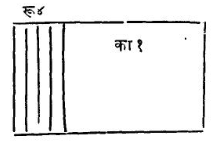
\includegraphics[scale=0.7]{graphics/Capture19.png}
\end{figure}
\vspace{-2mm}

 अथ शेषक्षेत्रे सम्पूर्णः कालको दर्शयितुमशक्यः~। यतो दीर्घभुजोऽत्र कालकमानम्~। स च यावत्तावच्चतुष्टयापनयनेन रूपचतुष्टयोनो दृश्यते~। अतो
रूपचतुष्टयोनं
कालकत्रयं प्रदर्श्यते~।
\vspace{-2mm}

\begin{figure}[h!]
    \centering
    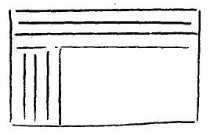
\includegraphics[scale=0.7]{graphics/Capture20.png}
\end{figure}
\vspace{-2mm}

 इह कालकेषु प्रत्येकं यावत्तावदङ्कतुल्यानि रूपाणि ४ न्यूनानि सन्तीति
कालकत्रयस्य जातानि कालकाङ्कगुणितानि तानि न्यूनानि १२~। अथ यदि
भावितक्षेत्रात्प्रथमतः कालकत्रयमपनीयते तर्हि कालकाङ्कतुल्यरूपैः ३ ऊनं यावत्तावतो
लघुभुजस्य मानं दृश्यते~। अतो रूपत्रयोनस्य यावत्तावतश्चतुष्टयं प्रदर्श्यते~।
\vspace{-2mm}

\begin{figure}[h!]
    \centering
    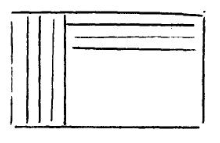
\includegraphics[scale=0.7]{graphics/Capture21.png}
\end{figure}
\newpage
%%%%%%%%%%%%%%%%%%%%%%%%%%%%%%%%%%%%%
%२२८ बीजगणिते\\
 इह यावत्तावत्सु प्रत्येक कालकाङ्क\textendash \,३\textendash \,तुल्यानि रूपाणि न्यूनानि सन्तीति
यावत्तावच्चतुष्टयस्य जातानि चतुर्गुणितानि न्यूनानि १२~। उभयथापि
वर्णाङ्काहतितुल्यै रूपैरूनं यावत्तावच्चतुष्टयं कालकत्रयं च क्षेत्रमध्ये प्रदर्शितं
भवति~। अथ
यदि सङ्कीर्णमेव यावत्तावच्चतुष्टयं कालकत्रयं प्रदर्श्यते तदैवं दर्शनं
भवति~।
\begin{table}[h!]
  \centering\renewcommand{\arraystretch}{0.8}
\begin{tabular}{|l|l|l|l|p{2.5cm}|}
\hline
 &  &  &  &  \\ \hline
 &  &  &  &  \\ \hline
 &  &  &  &  \\ \hline
 &  &  &  &  \\ 
 &  &  &  &  \\ 
 &  &  &  &  \\ 
  &  &  &  &  \\ \hline
\end{tabular}
\end{table}

 इह \,ये \,कोणे \,कोष्ठका \,उत्पद्यन्ते \,सा \,वर्णाङ्काहतिरेव~। अथ \,वर्णाङ्काहतितुल्यास्ते
कोणकोष्ठका यदि कालकत्रयमध्ये गुण्यन्ते तदा यावत्तावच्चतुष्टयार्थं
तावन्त एव कोष्ठका
अपेक्षिताः यदि तु यावत्तावच्चतुष्टयमध्ये गण्यन्ते तदा कालकत्रयार्थं
तावन्त एव कोष्ठका
अपेक्षिताः~। उभयथापि \,क्षेत्रशेषखण्डे \,यदि \,वर्णाङ्काहतितुल्याः \,कोष्ठका \,गृह्यन्ते \,तदा सम्पूर्णं यावत्तावच्चतुष्टयं सम्पूर्णं कालकत्रयं च भवति~। भावितसमपक्षे च
यावच्चतुष्टयं कालकत्रयं रूपद्वयं च वर्तते~। अतः क्षेत्रशेषे
वर्णाङ्काहत्या
रूपद्वयेन च भाव्यम्~। कथमन्यथा द्वितीयपक्षो भावितसमः स्यात्~।
तस्माद्भावितक्षेत्रान्तर्गते कोणस्थे लघुक्षेत्रे वर्णाङ्काहतिरूपैक्यतुल्याः
कोष्ठकाः सन्तीति सिद्धम्~।
ते च तस्य लघुक्षेत्रस्य फलम्~। तद्भुजयोर्वधाज्जातम्~। अत इष्टमेकभुजं
प्रकल्प्य
तेन क्षेत्रफले भक्ते यल्लभ्यते तद्द्वितीयो भुजः स्यात्~। अथाभ्यां
भुजाभ्यां
यावत्तावत्कालकयोर्माने ज्ञातुं न किञ्चित्काठिन्यमस्ति~। तथा हि यतो
यावत्तावदङ्कतुल्यै रूपैरूनः कालकोऽस्य लघुक्षेत्रस्य को भुजोऽस्त्यतोऽसौ
यावत्तावदङ्कतुल्यै रूपैर्युतः
सन्कालकमानं स्यात्~। एवं कालकाङ्कतुल्यै रूपैरूनो यावत्तावद्वर्णो लघुक्षेत्रस्य
द्वितीयो भुजोऽस्त्यतोऽसौ कालकाङ्कतुल्यै रूपैर्युतः सन्यावत्तावन्मानं
स्यात्~। अत्रेष्टं
यदि कालकखण्डात्मकस्य भुजस्य मानं कल्प्यते तदानेन क्षेत्रफले भक्ते
यत्फलं
तद्यावत्तावत्खण्डात्मकस्य द्वितीयभुजस्य मानं स्यात्~। अत इष्टं
यावत्तावदङ्कयुतं
कालकमानं स्यात्~। (फलं कालकाङ्कयुतं यावत्तावन्मानं स्यात्~।) यदि त्विष्टं
\newpage
%%%%%%%%%%%%%%%%%%%%%%%%%%%%%%%%%%%%%%5
\noindent यावत्खण्डात्मकस्य भुजस्य मानं कल्प्यते तदा फलं कालकखण्डात्मकस्य भुजस्य
 मानं स्यात्~। अत इष्टं कालकाङ्कयुतं यावत्तावन्मानं स्यात्~। फलं
यावत्तावदङ्कयुतं कालकमानं स्यादिति~। अत उपपन्नमिष्टफलाभ्यां स्वेच्छया संयुतौ 
वर्णाङ्कौ व्यत्ययाद्वर्णयोर्माने ज्ञातव्ये इति~। \\

\vspace{-4mm}
 अथवान्यथोपपत्तिः~। भावितक्षेत्रान्तर्गतक्षेत्रल्य भुजयोर्माने अन्यवर्णौ
कल्पिते दर्शनम्
\vspace{-4mm}

\begin{figure}[h!]
    \centering
    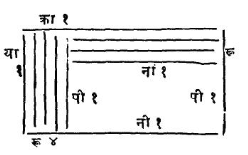
\includegraphics[scale=.7]{graphics/Capture22.png}
\end{figure}
\vspace{-2mm}

 इह नीलको यावत्तावदङ्कतुल्यै रूपैर्युतो जातं कालकमानं नी १ रू ४~। एवं
 पीत-काङ्कः कालकाङ्कतुल्यै रूपैर्युतो जातं यावत्तावन्मानं पी १ रू ३~। एवं क्रमेण जाते यावत्तावत्कालकमाने पी १ रू ३~। नी १ रू ४~। आभ्यां पक्षयोरनयोः $\begin{matrix}
\vspace{-1mm}
\mbox{{या ४ का ३ रू २}}\\
\vspace{-1mm}
\mbox{{याकाभा १ ~~~~}}
\vspace{1mm}
\end{matrix}$ यावत्तावत्कालकावुत्थाप्य जातमुपरिगपक्षे पी ४ रू १२ नी ३ रू १२ रू २~। द्वितीयपक्षे तु यावत्कालकयोर्वधोऽस्तीति गुणनार्थं न्यासः $\begin{matrix}
\vspace{-1mm}
\mbox{{पी १~। नी १ रू ४}}\\
\vspace{-1mm}
\mbox{{रू ३~। नी १ रू ४}}
\vspace{2mm}
\end{matrix}$ गुणनाज्जातो द्वितीयपक्षः पी नी भा १ पी ४ नी ३ रूप १२~। एवं पक्षौ $\begin{matrix}
\vspace{-1mm}
\mbox{{पी ४ रू १२ नी ३ रू रू १२ रू २}}\\
\vspace{-1mm}
\mbox{{पीनीभा १ पी ४ नी ३ रू १२ ~~~}}
\vspace{1mm}
\end{matrix}$
\newpage
%%%%%%%%%%%%%%%%%%%%%%%%%%%%%%%%%%%%%%%%%%%%%%%%%%%%%
 अथ नीलकयोः पीतकयोश्च तुल्यत्वात्समशोधनेन नाशे जातौ पक्षौ 
\vspace{-2mm} 

\begin{center}
$\begin{matrix}
\vspace{-1mm}
\mbox{{रू १२ रू १२ रू २}}\\
\vspace{-1mm}
\mbox{{नीपीभा १ रू १२ ~}}
\vspace{1mm}
\end{matrix}$ 
\end{center}
\vspace{-2mm} 

अथोभयपक्षयोर्वर्णाङ्काहतितुल्यरूपाणां समशोधनेन नाशे जातौ रू १२ रू २~।
अत्रोर्ध्वपक्षे वर्णाङ्काहतितुल्यानि रूपाणि सन्ति यथास्थितरूपाणि नीपीभा १ च
सन्ति~। अतो वर्णाङ्काहतिरूपैक्यमुपरिगपक्षे रू १४~। अधःपक्षे तु नीपीभा १~।
पक्षयोः समत्वाद्यदेव नीलकपीतकभावितं तदेव वर्णाङ्काहतिरूपैक्यमिति
सिद्धम्~। अतो नीलकपीतकयोरेकतरस्येष्टं मानं प्रकल्प्य तेन वर्णाङ्काहतिरूपैक्ये भक्ते
यल्लभ्यते तद्द्वितीयस्य मानं स्यात्~। एवं सिद्धमिष्टतत्फले अन्तःक्षेत्रभुजयोर्माने इति~।\\
 
 \vspace{-4mm}
 अथ यावत्कालकमनयोः पीतकनीलकौ स्वस्वमानेनोत्थाप्य वा प्राग्वद्वेष्टतत्फलाभ्यां
स्वेच्छया संयुतौ वर्णाङ्कौ व्यत्ययाद्वर्णयोर्माने भवत इत्युपपद्यते~। तदेवं
भावितसमे द्विती-यपक्षे वर्णाङ्कयो रूपाणां च धनत्वे प्रतिपादितम्~। यत्र तु
वर्णाङ्कावृणं रूपाणि तु धनं तत्रान्यथा संस्था भवति~। तथा हि कल्पितौ पक्षौ $\begin{matrix}
\vspace{-1mm}
\mbox{{या ४ं का ३ं रू ३०}}\\
\vspace{-1mm}
\mbox{{याकाभा १ ~~~~~}}
\vspace{1mm}
\end{matrix}$~। अत्र पक्षयोर्यावच्चतुष्टये कालकं त्रये च क्षिप्ते जातौ $\begin{matrix}
\vspace{-1mm}
\mbox{{या ० का रू ३० ~~~~~~}}\\
\vspace{-1mm}
\mbox{{या का भा १ या ४ का ३}}
\vspace{1mm}
\end{matrix}$~। अत्र स्वाङ्कगुणाभ्यां वर्णाभ्यां युक्तस्य भावितस्य यन्मानं तदेव रूपाणामपीति सिद्धम्~। तस्य दर्शनम्
\vspace{-2mm}

\begin{figure}[h!]
    \centering
    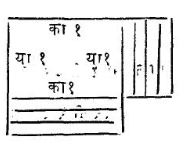
\includegraphics[scale=0.7]{graphics/Capture23.png}
\end{figure}
\newpage
%%%%%%%%%%%%%%%%%%%%%%%

 एतद्द्वितीयपक्षस्य रूपात्मकस्य मानम्~। अत्र रिक्तकोणे वर्णाङ्काहतितुल्याः
कोष्ठका यदि क्षिप्यन्ते तदैवं भवति~।
\vspace{-2mm}

\begin{figure}[h!]
    \centering
    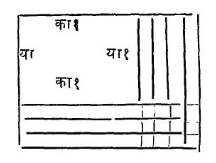
\includegraphics[scale=0.7]{graphics/Capture24.png}
\end{figure}
\vspace{-2mm}

 अस्य महतः क्षेत्रस्य वर्णाङ्काहतिरूपैक्यफलमस्ति~। पूर्वं यस्य
क्षेत्रस्य वर्णाङ्काहतिरूपैक्यं फलं तत्क्षेत्रं भावितक्षेत्रान्तर्गतं कोणस्थमासीत्~। इदानीं
तु भावितक्षेत्रमेव
तदन्तर्गतकोणस्थं भवतीति विशेषः~। महतः क्षेत्रस्यैकं भुजमिष्टं
प्रकल्प्यानेन क्षेत्रफले
भक्ते प्राग्वद्वितीयभुजमानं भवेत्~। इहेष्टं तथा कल्पनीयं यथा
स्वयमेकतरवर्णाङ्कादधिकं
भवेत्तत्फलं चान्यवर्णाङ्कादधिकं भवेत्~। अथाभ्यां भुजाभ्यां वर्णमानं
साध्यम्~।
तद्यथा\textendash \,इह कालकाङ्कयुतो यावत्तावद्वर्ण एको भुजोऽस्ति~। अतोऽसौ
कालकाङ्केनोनो
यावत्तावन्मानं स्यात्~। एवं यावत्तावदङ्कयुतः कालकोऽस्य क्षेत्रस्य
द्वितीयभुजोऽस्ति~।
अतोऽसौ यावत्तावदङ्ककोनः कालकमानं स्यात्~। अत्र भुजौ त्विष्टतत्फले~। अत
इष्टतत्फले
वर्णाङ्कोने व्यत्ययान्माने भवत इति यद्यपि वक्तुमुचितं तथापि प्रकृते
वर्णाङ्कावृणगताविति तद्योग एव कृते सतीष्टतत्फले वर्णाङ्कोने भवत इति तथा नोक्तम्~।\\

\vspace{-4mm}
 अथ यत्र वर्णाङ्कौ धनं रूपाणि त्वृणं तत्र द्वैविध्यमस्ति~। अन्योन्यभुजतो
न्यूनो
वर्णाङ्कावित्येकः प्रकारः~। अन्योन्यभुजतोऽधिको वर्णाङ्काविति द्वितीयः~।
तत्र प्रथमे
प्रागु-क्तयुक्त्या भावितक्षेत्रान्तर्गतलघुक्षेत्रे वर्णाङ्काहत्या रूपोनया
भाव्यम्~। सा च
वर्णाङ्काहती रूपयुता सती रूपोना भवति~। रूपाणामृणत्वात्~। अतोऽत्रापि
वर्णाङ्का
हतिरूपैक्यमेव भावितक्षेत्रान्तर्गतक्षेत्रस्य फलं भवति~। अतः
प्रथमप्रकारे प्राग्वदेवोपपद्यते~। द्वितीयप्रकारे त्वन्यभुजमानाद्वर्णाङ्कोऽधिकोऽस्तीति
स्वाङ्कगुणवर्णस्य मानं भावितक्षेत्रमतिक्रम्य बहिरपि भवति~। यतो भावितक्षेत्रे कालकमानतुल्या एव
यावद्वर्णाः
\newpage
%%%%%%%%%%%%%%%%%%%%%%%%%%
\noindent सम्भवन्ति नाधिकाः~। एवं यावत्तावन्मानतुल्या एव कालकाः सम्भवन्ति नाधिकाः~। अथ तत्र स्वाङ्कगुणवर्णयोर्दर्शनम्~।
\vspace{-2mm}

\begin{figure}[h!]
    \centering
    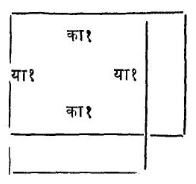
\includegraphics[scale=0.7]{graphics/Capture25.png}
\end{figure}
\vspace{-2mm}

 अत्र भावितक्षेत्रं यदि स्वाङ्कगुणयावत्तावन्मध्ये गण्यते तर्हि
स्वाङ्कगुणकालकमानार्थमन्यद्भावितक्षेत्रमपेक्षितम्~। यदि तु स्वाङ्कगुणकालकमानमध्ये
गण्यते तर्हि
स्वाङ्कगुणयावत्तावन्मानार्थमन्यद्भावितक्षेत्रमपेक्षितम्~। उभयथापि
भावितक्षेत्रलिखितक्षेत्रयोर्योगे स्वाङ्कगुणवर्णौ भवतः~। अतो
रूपैर्लिखितक्षेत्रसमैर्भाव्यम्~। कथमन्यथा
स्वाङ्कगुणवर्णौ रूपैरूनौ भावितसमौ भवतः~। अथ लिखितं रूपात्मकं क्षेत्रं
रिक्तकोणे यदि पूर्यते तदैवं भवति~।
\vspace{-2mm}

\begin{figure}[h!]
    \centering
    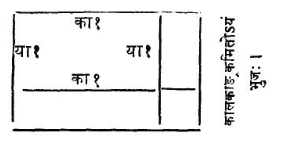
\includegraphics[scale=0.7]{graphics/Capture26.png}
\end{figure}
\vspace{-10mm}

\begin{center}
यावदङ्कमितोऽयं भुजः ~~~~
\end{center}

 अत्र वर्णाङ्काहतिः क्षेत्रफलमस्ति~। पूर्वलिखितक्षेत्रे तु रूपाण्येव~। अतो
वर्णाङ्काहती रूपैरूना सती भावितक्षेत्रबहिःकोणस्थस्य लघुक्षेत्रस्य फलं
भवति~। तच्च वर्णाङ्काहतिरूपैक्यकरणादेव सम्पद्यते~। यतोऽत्र
रूपाणामृणत्वाद्वर्णाङ्काहतेश्च धनत्वात् 

\newpage
%%%%%%%%%%%%%%%%%%%%%%%%%%%%%%%%%%%%
\noindent \hyperref[3]{\textbf{धनर्णयोरन्तरमेव योगः}} इति योगे कृते रूपैरूनैव वर्णाङ्काहतिर्भवति~। अथ
लघुक्षेत्रस्यैकं भुजमिष्टं प्रकल्प्यानेन क्षेत्रफले भक्ते द्वितीयभुजमानं स्यात्~।
अथाभ्यां भुजाभ्यां वर्णमाने साध्ये~। ते यथा\textendash \,इह यावत्तावन्मानोनः कालकाङ्कोऽस्य लघुक्षेत्रस्यैको भुजोऽस्ति~। अतोऽनेन कालकाङ्क ऊनः
सन्यावत्तावन्मानं
भवेत्~। एवं कालकमानेनोनो यावत्तावदङ्कोऽस्य लघुक्षेत्रस्य
द्वितीयभुजोऽस्ति~।
अतोऽनेन यावत्तावदङ्क ऊनः सन्कालकमानं भवेत्~। भुजौ त्विष्टतत्फले~।
तत्फलेष्टे
वा~। अत इष्टतत्फलाभ्यां स्वेच्छयोनौ वर्णाङ्कौ व्यत्ययान्माने भवत
इत्युपपन्नम्~।
तदेवमयं निकृष्टोऽर्थः~। यदि भावितसमे पक्षे रूपाणि धनं
स्युस्तदेष्टतत्फलाभ्यां
वर्णाङ्को धनमृणं वा यथावत्संयुक्तावेव व्यत्ययान्माने भवतः~। यदि तु
रूपाण्यृणं
स्युस्तदेष्टतत्फलाभ्यां स्वेच्छया संयुतावूनौ च वर्णाङ्कौ व्यत्ययान्माने
भवतः~।
अस्मिन्पक्षे वर्णाङ्कयोर्धनत्वमेव~। न हि त्रयाणामृणत्वे वर्णमानं धनं
सम्भवति~।
ऋणे वा वर्णमाने लोकानां प्रतीतिरस्ति~। अत्रापरो विशेषः~। यत्र संयुक्तवर्णाङ्कजे ऊनवर्णाङ्कजे च माने उपपन्ने भवतस्तदत्रोभे अपि ग्राह्ये~।
अन्यत्र तु ये
उपपन्ने ते एव ग्राह्मे इति~। इति भावितोपपत्तिः~। अत्र त्रयाणामपि धनत्वे
चतुस्त्रिगुणयो राश्योरित्युदाहरणं प्रदर्शितम्~॥~१८५~॥~\\

\vspace{-2mm}
 अथ यत्र वर्णाङ्कौ धनं रूपाणि त्वृणं स्युस्तादृशमुदाहरणमनुष्टुभाह\textendash

\phantomsection \label{186}
\begin{quote}
    \eg 
     द्विगुणेन कयो राश्योर्घातेन सदृशं भवेत्~।\\
 दशेन्द्राहतराश्यैक्यं द्व्यूनषष्टिविवर्जितम्~॥~१८६~॥

\end{quote}

 स्पष्टोऽर्थः~। गणितमाकरे स्पष्टम्~॥~१८६~॥\\

\vspace{-2mm}
 अथ यत्र वर्णाङ्कावृणं रूपाणि तु धनं स्युस्तादृशमुदाहरणमनुष्टुभाह\textendash

\phantomsection \label{187}
\begin{quote}
    \eg 
     त्रिपञ्चगुणराशिभ्यां युक्तो राश्योर्वधः कयोः~।\\
 द्विषष्टिप्रमितो जातो राशी त्वं वेत्सि चेद्वद~॥~१८७~॥

\end{quote}

 स्पष्टोऽर्थः~। गणितमाकरे स्पष्टम्~।
\newpage
%%%%%%%%%%%%%%%%%%%%%%%%%%%%%%%%%%%%%%%%%%%%%5
अथ यत्र रूपाणामृणत्वे प्रकारद्वयेनोत्पन्नमानयोरेकतरे एवोपपन्ने
भवतस्तादृशमुदाहरणं पूर्वचतुर्थमस्तीति तदेव प्रदर्शयति\textendash \,\hyperref[184]{\textbf{यौ राशी किल या च राशिनिहतिः}} इत्यादि~। गणितं स्पष्टमाकरे~॥~१८७~॥

\begin{quote}
{\qt दैवज्ञवर्यगणसन्ततसेव्यपार्श्वबल्लालसञ्ज्ञगणकात्मजनिर्मितेऽस्मिन्~।\\
 बीजक्रियाविवृतिकल्पलतावतारेऽभूद्भावितं सकलमेतदनेकवर्णे~॥~}
\end{quote} 

\begin{center}
 इति श्रीसकलगणकसार्वभौमश्रीबल्लालदैवज्ञसुतकृष्णगणकविरचिते \\ बीजक्रियाविवृतिकल्पलतावतारेऽनेकवर्णे भावितविवरणम्~। \\
    \vspace{4mm}
 
 अत्र ग्रन्थसङ्ख्या १४०~। एवमादितो
ग्रन्थसङ्ख्या ४४५८~।\\ 
\vspace{2mm}

इत्यनेकवर्णसमीकरणविवरणं समाप्तम्~॥~११~॥\\
    \vspace{10mm}
    \rule{0.3\linewidth}{0.5pt}\\
    \vspace{-5mm}
    \rule{0.3\linewidth}{0.5pt}
\end{center}
\newpage
%%%%%%%%%%%%%%%%%%%%%%%%%%%%%%%%%%%%%%%%%%%%%%
\phantomsection \label{ch12}
\begin{center}
{\LARGE \textbf{ग्रन्थसमाप्तिः~।}}\\
    \rule{0.2\linewidth}{0.5pt}\\
\end{center} 

अथास्य ग्रन्थस्य प्रचारार्थं गुरूत्कर्षकथनरूपं मङ्गलमाचरन्ग्रन्थसमाप्तिं
वसन्ततिल-कयाह\textendash
\begin{quote}
    \ab 
     आसीन्महेश्वर इति प्रथितः पृथिव्याम्\\
 आचार्यवर्यपदवीं विदुषां प्रयातः~।\\
 लब्ध्वावबोधकलिकां तत एव चक्रे\\
 तज्जेन बीजगणितं लघु भास्करेण~॥~१~॥
\end{quote}

लघ्विति च्छेदः स्पष्टोऽर्थः~॥~१~॥~\\

\vspace{-2mm}
 ननु बीजगणितानि ब्रह्मगुप्तादिभिः प्रतिपादितानि सन्ति
तत्किमर्थमाचार्यैर्यतितमिति शङ्कायामिन्द्रवज्रयोत्तरमाह\textendash
\begin{quote}
    \ab 
     ब्रह्माह्वयश्रीधरपद्मनाभबीजानि यस्मादतिविस्तृतानि~।\\
 आदाय तत्सारमकारि नूनं सद्युक्तियुक्तं लघु शिष्यतुष्ट्यै~॥~२~॥~
\end{quote}

अत्रापि लघ्विति च्छेदः~। शेषं स्पष्टम्~॥~२~॥~\\

\vspace{-2mm}
 कथमिदं लघ्वित्याशङ्कायामाहानुष्टुप्पूर्वार्धेन\textendash
\begin{quote}
    \ab 
     अत्रानुष्टुप्सहस्रं हि ससूत्रोद्देशके मितिः~॥~३~॥
\end{quote}

 हि यतोऽत्र ससूत्रोद्देशके बीजगणितेऽनुष्टुप्सहस्रमितिः पूर्वबीजगणितेषु
तु सहस्रद्वयत्रयादिमितिरस्ति अतो लघ्विदमित्यर्थः~।\\

\vspace{-2mm}
 नन्विदमपि विस्तृतमस्ति~। क्वचित्क्वचिदेकस्मिन्नेव विषय
उदाहरणबाहुल्योक्तेरिति शङ्कायामनुष्टुभोत्तरपूर्वार्धाभ्यामाह\textendash
\thispagestyle{empty}
\afterpage{\fancyhead[CE] {बीजगणिते}}
\afterpage{\fancyhead[CO]{ग्रन्थसमाप्तिः}}
\afterpage{\fancyhead[R]{\thepage}}
\afterpage{\fancyhead[L]{}}
\cfoot{}
\newpage%%%%%%%%%%%%%%%%%%%%%%%%%%%%%%%%%%२३६
\begin{quote}
    \ab
      क्वचित्सूत्रार्थविषयं व्याप्तिं दर्शयितुं क्वचित्~।\\
 क्वचिच्च कल्पनाभेदं क्वचिद्युक्तिमुदाहृतम्~॥~\\
 क्वचित्सूत्रार्थविषयं दर्शयितुमुदाहृतम्~॥~४~॥~
\end{quote}

 यथा भाविते \hyperref[182]{\textbf{चतुस्त्रिगुणयो राश्योः}} इति \hyperref[186]{\textbf{द्विगुणेन कयो राश्योः}} इति \hyperref[187]{\textbf{त्रिपञ्चगुणराशिभ्याम्}} इति \hyperref[184]{\textbf{यौ राशी किल या च राशिनिहतिः}}
इत्युदाहरणचतुष्टयमुदाहृतम्~। न ह्येकस्मिन्नुदाहृते \hyperref[185]{\textbf{भावितं पक्षतोऽभीष्टात्}} इति सूत्रस्यार्थः
सर्वोऽपि विषयी भवति~। तस्मादशेषं सूत्रार्थं
दर्शयितुमुदाहरणचतुष्टयमप्यावश्यकम्~।
एवं क्वचिद्व्याप्तिं दर्शयितुमुदाहृतम्~। यथा\textendash \,\hyperref[96]{\textbf{पञ्चकशतदत्तधनात्}} इत्युदाहृत्य \hyperref[97]{\textbf{एकशत(दत्त)धनतः}} इति तादृशमेव पुनरुदाहृतम्~। इदं यदि नोदाहृते तर्हि स्वकृते प्रकारविशेषे मन्दानां विश्वासो न भवेदित्येतदावश्यकम्~। एवं
कल्पनाभेदं दर्शयितुं \hyperref[93]{\textbf{एको ब्रवीति मम देहि}} इत्युदाहरणमेकवर्णसमीकरण उदाहृतम् एवं
विविधयुक्तिप्रदर्शनार्थमपि बहुषु स्थलेषूदाहृतमस्ति~। यस्मादयं विस्तारो
न दोषाय~॥~४~॥~\\

\vspace{-2mm}
 ननु पूर्वबीजेषूदाहरणानि बहूनि सन्तीह तु स्वल्पान्येवोक्तानीति न सकलोदाहरणावगमः स्यादत आह\textendash
\begin{quote}
    \ab 
     न ह्युदाहरणान्तोऽस्ति स्तोकमुक्तमिदं यतः~॥~५~॥
\end{quote}
 
 हि यत उदाहरणान्तो नास्ति~। अत इदं स्तोकं स्वल्पमुक्तम् पूर्वबीजेष्वपि सकलान्युदाहरणानि नैवोक्तानि~। तेषामनन्तत्वेन वक्तुमशक्यत्वात्
अतोऽल्पैरप्युदाहरणैर्विविधयुक्तिषु प्रदर्शितासु शेषं व्यर्थमिति भावः~॥~५~॥\\

\vspace{-2mm}
 नन्वत्र स्वल्पमुक्तं पूर्वबीजानि त्वतिविस्तृतान्यतस्तान्येव
मन्दप्रयोजनायालमित्याशङ्कायामाह~। यतः\textendash
\begin{quote}
    \ab 
    दुस्तरः स्तोकबुद्धीनां शास्त्रविस्तारवारिधिः~।\\
 अथवा शास्त्रविस्तृत्या किं कार्यं सुधियामपि~॥~६~॥~
\end{quote}

\newpage
%%%%%%%%%%%%%%%%%%%%%%%%%%%%%%%%%%%%%%%%%%%%%%
 यो हि विस्तारः स मन्दार्थं सुध्यर्थं वा~। नाद्यः~। यतः
शास्त्रविस्तारवारिधिः स्तोक-बुद्धीनां मन्दानां दुस्तरः~। दुर्बोध इति यावत्~। यतो महति
ग्रन्थे प्रत्युत किं कुत्रास्ति किमत्र कर्तव्यमित्यनवबोधेनेतिकर्तव्यतामूढा एव
ते स्युः~। नान्त्यः~। सुधियामपि शास्त्र-विस्तृत्या किं कार्यम्~। यतस्ते
कल्पनासमर्थाः~। ननु
लघ्वपि बीजं मन्दार्थं सुध्यर्थं वा~। नाद्यः~। तैर्ज्ञातुम् अशक्यत्वात्~। नान्त्यः~।
तेषां कल्पकत्वादिति चेन्न~। स्वल्पग्रन्थस्य मन्दानामभ्याससाध्यत्वान्न
तावत्प्रथमपक्षे दोषः~॥~६~॥\\

\vspace{-2mm}
 द्वितीयेऽपि न दूषणमित्याह\textendash
\begin{quote}
    \ab 
 उपदेशलवं शास्त्रं कुरुते धीमतो यतः~।\\
 तत्तु प्राप्यैव विस्तारं स्वयमेवोपगच्छति~॥~७~॥~
\end{quote}

 यतः शास्त्रं धीमत उपदेशलवं कुरुते~। तत्तु शास्त्रं सुधियं प्राप्य स्वयमेव
विस्तारम् उपगच्छति~। न हि सुधियोऽपि किञ्चिदप्यनधीत्य जानन्ति~। अत इदं
मदुक्तं सुधीमन्दसाधारणप्रयोजनायेति सर्वैरपि पठनीयमिति भावः~॥~७~॥~\\

\vspace{-2mm}
 ननु शास्त्रं सुधियं प्राप्य स्वयमेव विस्तारमुपगच्छतीति 
कथमित्याशङ्कायां सदृष्टान्तम् आह\textendash
\begin{quote}
    \ab 
     जले तैलं खले गुह्यं पात्रे दानं मनागपि~।\\
 प्राज्ञे शास्त्रं स्वयं याति विस्तारं वस्तुशक्तितः~॥~८~॥~
\end{quote}

 स्पष्टोऽर्थः~॥~८~॥~\\
\begin{center}
    \rule{0.3\linewidth}{0.5pt}\\
    \vspace{-5mm}
    \rule{0.3\linewidth}{0.5pt}
\end{center}
\newpage
%%%%%%%%%%%%%%%%%%%%%%%%%%%%%%%%%%%%%%%%%%%
\phantomsection \label{ch13}
\begin{center}
{\LARGE \textbf{हस्तलिखितप्रतीनां समाप्तिः~।}}\\
    \rule{0.4\linewidth}{0.5pt}\\
\end{center}

क इति सञ्ज्ञित आनन्दाश्रमग्रन्थसङ्ग्रहालयस्थे ग्रन्थसमाप्तिरेवं विद्यते\textendash

\phantomsection \label{End8}
\begin{quote}
    \qt 
    कश्चित्किञ्चित्स्वं गृहीत्वा प्रयागाद्यातः काशी तत्र तत्पञ्चनिघ्नम्~।\\
कृत्वा पञ्चाशल्लवं विंशदंशनिघ्नं तस्य ब्राह्मणेभ्यः प्रदत्वा~॥~८~॥\\
शम्भोः पूजां चैकमूलेन कृत्वा राशेर्धृत्यंशेन पञ्चाहतेन~।\\
कौशेयादीन् सङ्गृहीत्वा दश स्वो जातस्तत्स्वं ब्रूहि बीजज्ञ तूर्णम्~॥
\end{quote}

नगगजभूपैः १६८७ प्रमिते शाके लिलेख यादवोऽभिज्ञः~।
मल्लारिजः शिवपूर्याम्~॥
\begin{center}
{\qt श्रीसाम्बसदाशिवार्पणमस्तु~।}\\
\end{center}
\vspace{-4mm}

\begin{quote}
    \qt 
\hspace{15mm} यादृशं पुस्तकं दृष्टं तादृशं लिखितं मया~।\\
\vspace{-7mm}

\hspace{15mm} यदि शुद्धमशुद्धं वा मम दोषो न विद्यते~॥
\end{quote}

स्वार्थं परार्थं च शके १७६७ विश्वावसुनामसंवत्सरे पौषशुद्धद्वितीयायां
भौमवासरे पुस्तकं समाप्तम्~।
\vspace{-2mm}

\begin{center}
{\qt श्रीसीतारामचन्द्रार्पणमस्तु~।\\
 श्रीगजाननः प्रसन्नः~।}
\end{center}

ख. इति सञ्ज्ञित आनन्दाश्रमग्रन्थसङ्ग्रहालयस्थे ग्रन्थसमाप्तिरेवं
विद्यते\textendash
\begin{quote}
    \qt 
 श्रीकृष्ण राम मधुसूदन दानवारे शौरे त्रिविक्रम गदाधर पद्मनाभ~।\\
 श्रीवत्स भक्तजनपालक विश्ववन्द्य लक्ष्मीपतेऽस्तु मम ते सततं प्रणामः~॥~१~॥\\
 शम्भो शशाङ्कधर भस्मविभूषिताङ्ग नन्द्यादिवन्दितपदद्वय भूतनाथ~।\\
 मूर्ध्ना धृतत्रिपथगार्द्रजटासमूह गौरीपतेऽस्तु सततं मम ते प्रणामः~॥~२~॥~\\
 हेरम्ब शङ्कर तनूद्भव वारणास्य बालार्कदीधितिसदृक्षशरीरकान्ते~।\\
 लम्बोदरैकरद विघ्ननिवारणैकहेतो मम प्रतिदिनं नतिराविरस्तु~॥~३~॥\\
 आदित्य भास्कर दिवाकर लोकबन्धो सप्ताश्व विश्वनयनान्ध्यहरारुणेश~।\\
 सिन्दूरधूसरकरप्रकरप्रभैकराशेऽस्तु ते मम मतिप्रकरः सदैव~॥~४~॥\\
 क्षीरोद्भवे कमलवासिनि विश्ववन्द्ये पद्मे रमे कमलशोभितहस्तपद्मे~।\\
 ब्रह्माच्युतेशहरसूनुदिवाकरादिवन्द्येऽस्तु ते मम प्रणामततिः सदैव~॥~५~॥~
\end{quote}

 शके १८१२ विकृतिनामसंवत्सरे मार्गशीर्षशुक्ल\textendash \,१४\textendash \,गुरौ हर्डीकरोपनामकविनायकेन लिखितमिदम्~।
\begin{center}
    ( ग्रन्थसङ्ख्या ) ४५००
\end{center}

\thispagestyle{empty}
\afterpage{\fancyhead[CE]{बीजगणिते}}
\afterpage{\fancyhead[CO]{हस्तलिखितप्रतीनां समाप्तिः}}
\afterpage{\fancyhead[R]{\thepage}}
\afterpage{\fancyhead[L]{}}
\cfoot{}
 
\newpage
%%%%%%%%%%%%%%%%%%%%%%%%%%%%%%%%%%%%
\pagestyle{fancy}
एवं स्वकृतस्यास्य बीजस्य गुणान्युक्त्या संस्थाप्योपसंहरति\textendash
\begin{quote}
    \ab 
      गणक भणतिरम्यं बाललीलावगम्यम्~।\\
 सकलगणितसारं सोपपत्तिप्रकारम्~॥~\\
 इति बहुगुणयुक्तं सर्वदोषैर्विमुक्तम्~।\\
 पठ पठ मतिवृद्ध्यै लघ्विदं प्रौढसिद्ध्यै~॥~६~॥~

\end{quote}

 गणकेति सम्बोधनम्~। भणतयः शब्दोस्तै रम्यम्~। पदलालित्ययुक्तमित्यर्थः~।
शेषं स्पष्टम्~॥~६~॥~
\begin{quote}
    \qt 
     अभूत्पृथिव्यां प्रथितो गुणौघैश्चिन्तामणिर्दैवविदां वरिष्ठः~।\\
 सम्पूजनानेहसि यस्य गौरी स्मृता स्तुता प्रत्यहमाविरासीत्~॥~१~॥~\\

\vspace{-5mm}
 तत्सूनवः पञ्च बभूवुरेषां ज्येष्ठोऽभिरामः किल रामनामा~।\\
 भविष्यदर्थज्ञतया हि यस्य विदर्भराजोऽपि निदेशवर्ती~॥~२~॥~\\

\vspace{-5mm}
 रामादभूतां सीतायां पुत्रौ कुशलवाविव~।\\
 त्रिमल्लो गोपिराजश्च गुणैः सर्वैः समन्वितौ~॥~३~॥~\\

\vspace{-5mm}
 त्रिमल्लसूनुर्जयति द्विजेन्द्रो बल्लालसञ्ज्ञः शितिकण्ठभक्तः~।\\
 यः सन्ततं रुद्रजपातिसङ्गाद्ब्राह्ममहो मूर्तमिवावभाति~॥~४~॥~\\

\vspace{-5mm}
 दैवज्ञवर्यगणसन्ततसेव्यपार्श्वबल्लालसञ्ज्ञगणकस्य सुतोऽस्ति कृष्णः~।\\
 रामानुजः स परमेश्वरतुष्टिहेतोर्बीजक्रियाविवृतिकल्पलतामकार्षीत्~॥~५~॥\\

\vspace{-5mm}
 यद्भास्करेण निजधामगुणातिरेकात्सम्पादितं सगुणवर्गघनं हि बीजम्~।\\
 तत्कृष्णभूमिमधिगम्य विचारवारिसंसिक्तमङ्कुरजनुष्यभवत्समर्थम्~॥~६~॥~

\end{quote}


\newpage
%%%%%%%%%%%%%%%%%%%%%%%%%%%%%%%%%%%%%%%%%%%%%%

\begin{quote}
    \qt
    यैर्यैः श्रमैर्विरचितोऽस्ति नवाङ्कुरोऽसौ~।\\
 तेषामभिज्ञ इह कः परमात्मनोऽन्यः~॥\\
 इत्थं विचिन्त्य जगदीश तवैव तुष्ट्यै~।\\
 सर्वज्ञ ते चरणयोर्निहितस्ततोऽयम्~॥~७~॥
\end{quote}
\vspace{-2mm}

{\qt इति श्रीवक्रतुण्डार्पणमस्तु~। ग्रन्थसङ्ख्या ४५००~।}\\
\vspace{-2mm}

 ग. इति सञ्ज्ञिते भाण्डारकरप्राच्यविद्यासंशोधनमन्दिरस्थे
ग्रन्थसमाप्तिरेवं विद्यते\textendash \\
\vspace{-4mm}

{\qt शके १७४७ पार्थिनामाब्द उत्तरायणे शशिऋतौ (शिशिरर्तौ) माघमासे शुक्लपक्षे १ भौमवासरे धनिष्ठानक्षत्रे वर्यान्योग एतच्छुभदिन इदं पुस्तकं
समाप्तम्~।\\
\vspace{-4mm}

श्रीजगदम्बार्पणमस्तु शुभं भवतु~॥ श्रीरस्तु~॥ श्रीराम~॥ श्रीकृष्ण श्रीहरि~॥}\\

\vspace{-2mm}
 घ. इति सञ्ज्ञिते ग्रन्थसमाप्तिर्न विद्यते त्रुटितत्वात्~॥\\

\vspace{-2mm}
 ङ. इति सञ्ज्ञिते कोल्ब्रूक इत्यभिधेनाङ्ग्लेन
लन्दनस्थग्रन्थसङ्ग्रहालयायार्पिते
ग्रन्थसमाप्तिरेवं विद्यते\textendash

{\qt इति श्रीभास्कराचार्यविरचिते सिद्धान्तशिरोमणौ बीजगणिताध्यायः समाप्तः~॥\\
\vspace{-4mm}

 ज्यारसभूधरचन्द्रे वर्षे रसद्विनृपे च शाके~॥ संवत् १७६१ वरषे अगहन सूदि
नवमी ९ शूक्रवासरे~॥ प्रयागमध्य अनूपसधिलेखकः इदं पूस्तकं लीख्यते~॥~छ~॥ छश्लोक १२२४~।}\\

\vspace{-2mm}
 च इति सञ्ज्ञिते काशीस्थकाॅलेजस्थेऽपि कसञ्ज्ञितस्थं \hyperref[End8]{\textbf{कश्चित्किञ्चित्}}
इदं पद्यं विद्यते~।

\vspace{5mm}
\begin{center}
    \rule{0.3\linewidth}{0.5pt}\\
\vspace{-5mm}
    \rule{0.3\linewidth}{0.5pt}
\end{center}

 \end{document}